% Outline: 3
\chapter{未知模型的求解}
\label{chap:rl-learning}

在导航网格中，智能体执行一次向右，就能记录下这一步的奖励和实际落脚位置，却仍然不知道“向右成功”这件事的真实概率。第\ref{chap:rl-planning}章的Bellman备份要求按转移概率对所有后继状态加权求期望；而一次真实交互只给出其中一个后果，无论重复多少次，单次观察都不等于那个条件期望本身。本章因此撤掉“转移表已知”的前提，让智能体在行动中学习。这里要同时回答两件紧密耦合的事：一次观察如何进入对长期回报的估计（学习），以及下一步应当去哪里取得足以纠正估计的新证据（探索）。

这里继续假定每一步都能观察到马尔可夫状态，一条经验记为四元组
$(s_t,a_t,r_t,s_{t+1})$，其中$r_t$是执行$a_t$后收到的奖励。贯穿全章的示例仍是宽4、高3的网格：起点$(1,1)$、终点$(4,3)$、障碍$(2,2)$；合法意图方向以$0.8$执行，两侧滑移各为$0.1$，滑移撞墙则留在原位。进入终点奖励为1，其他非终止步为$-0.04$，终点之后奖励为0，折扣$\gamma=0.9$。后文另设的短链和老虎机都会明确说明改动了哪些设定，不能把它们的手算结果当成整个随机网格的解。

同一条$(s,a,r,s')$经验其实有三种截然不同的用法，这也对应三类可以分别学习的对象。若想以后回答“在这里向右好还是向上好”，可以学习动作价值$Q(s,a)$，为每个动作预测长期回报；若想让系统直接根据当前位置输出动作，可以学习策略$\pi(a\mid s)$，调整各动作的选择概率；若想在脑中试算一条尚未真正执行的路线，则可以学习环境模型，预测给定动作后的落点分布与奖励。一句话概括：价值回答“这个行动值多少”，策略决定“下一步怎样行动”，模型预测“采取行动后会发生什么”。学会其中任何一种，都不代表自动掌握了另外两种。

学习之前还要先约定允许使用哪些表示。例如动作价值既可以逐格存成一张表，也可以由一组跨状态共享的参数算出；表示形式一旦确定，改变参数就对应在一族候选函数中挑选。用$\Theta_Q,\Theta_\pi,\Theta_{\mathrm{env}}$分别表示三者允许的参数范围，三类候选函数写为$\mathcal H_Q=\{Q_{\bm\theta}:\bm\theta\in\Theta_Q\}$、$\mathcal H_\pi=\{\pi_{\bm\theta}:\bm\theta\in\Theta_\pi\}$和$\mathcal H_{\mathrm{env}}=\{(\widehat T_{\bm\phi},\widehat R_{\bm\phi},\ldots):\bm\phi\in\Theta_{\mathrm{env}}\}$。这些集合划定学习时可以选择的范围，而训练结束后真正得到的那个具体函数才是学习产物。

交互记录组$D$由行动方式与采集协议共同生成，相邻记录通常相互依赖，并不是一筐独立抽签。因此学习规则除了选择表示，还必须完整规定：怎样从记录构造更新目标、怎样修改参数、何时停止，以及最终如何从训练产物产生动作。例如存下“这次向右没成功”之后，算法仍要决定究竟是降低向右的价值估计、调整向右的选择概率，还是更新向右成功概率的模型——同一个事实在三种用法下导向三种不同更新。后文会分别推导这些操作。

从同一条经验出发，既可以直接更新价值或策略，也可以先拟合一个环境模型、再借助它的预测完成更新。表\ref{tab:rl-learning-four-interfaces}按两个问题固定四种组合：改进时是否查询学习到的模型；执行时动作主要来自价值比较（或规划），还是来自一份参数化策略。需要强调，“无模型”只表示这次更新不依赖学得的环境转移预测，绝不意味着系统里没有价值函数或神经网络。反过来，模型虽然允许反复试算没有真正发生的后果，却也可能把同一个预测错误反复放大；显式策略能省去部署时的动作搜索，却要求先找到可靠的参数更新方向。后文还会大量把策略与价值估计配合使用，这种配合可以出现在多种组合中。

其中，“基于模型的价值学习”一节把两种做法放在一起讨论：用模型生成经验来更新价值函数，以及在每次执行动作前用模型预测并比较候选动作或轨迹。后一种做法属于在线规划，可以只计算候选轨迹的预计回报，而不训练独立的价值函数。两者都由价值比较或规划结果产生动作；“基于模型的策略优化”一节则讨论如何用模型训练一份参数化策略，供执行时直接调用。

\begin{table*}[t]
  \centering
  \small
  \begin{tabularx}{\linewidth}{>{\raggedright\arraybackslash}p{26mm} >{\raggedright\arraybackslash}X >{\raggedright\arraybackslash}X >{\raggedright\arraybackslash}X}
    \toprule
    主要改进接口 & 是否查询学习模型 & 价值承担的作用 & 最终动作来源与例子 \\
    \midrule
    无模型价值学习 & 不查询转移模型 & 比较动作的长期回报 & 根据$Q$比较动作，并保留必要试验 \\
    无模型策略优化 & 不查询转移模型 & 帮助判断策略应向哪个方向改变 & 从训练后的参数策略采样或输出动作 \\
    基于模型的价值学习 & 查询模型以模拟、前瞻或搜索 & 更新动作值，或给候选路线评分 & 根据更新后的$Q$或当前规划结果选动作 \\
    基于模型的策略优化 & 查询模型以求导或生成训练经验 & 为模型中的策略训练估计长期回报 & 调用训练后的参数策略 \\
    \bottomrule
  \end{tabularx}
  \caption{四种求解组合。分类依据是交互记录、训练目标与动作接口之间的实际依赖，而不是系统里是否出现过预测网络。}
  \label{tab:rl-learning-four-interfaces}
\end{table*}

学习这些更新，先要有可用经验，所以我们从动作选择与探索进入，再分别讨论价值和策略的学习。理解单步更新后，就能进一步看模型如何提供模拟经验或求导路径，以及一段多步行为怎样作为一次高层决策。最后需要检查，有限真实样本支持什么保证，实验又怎样计量样本与计算。图\ref{fig:rl-learning-map}展示这些关系。本章推导主要用到样本均值、条件期望、线性代数和链式法则；遇到新的统计结构时，会在它所解决的问题中说明其用途和条件。

\begin{figure}[htbp]
  \centering
  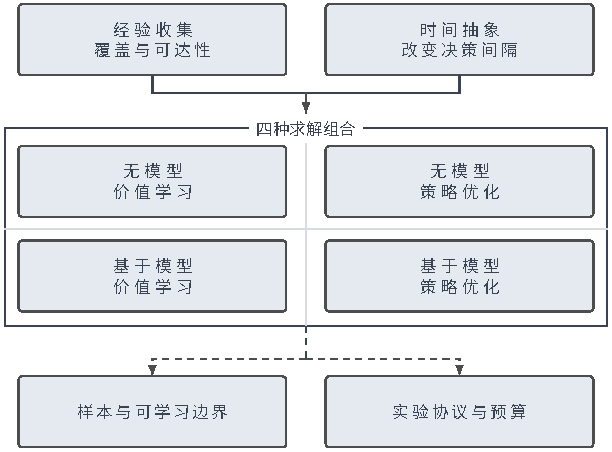
\includegraphics[width=103.618mm]{figures/10-reinforcement-learning/01-problems-and-solving/tikz/rl-learning-map.pdf}
  \caption{本章的问题关系。实线表示经验收集和时间抽象与四种求解接口之间的依赖或组合关系，虚线表示统一的分析与评价口径；四种求解接口没有先后执行关系。}
  \label{fig:rl-learning-map}
\end{figure}

% Outline: 3.1
\section{支持策略改进的经验收集}
\label{sec:rl-learning-experience}

在网格中，如果当前策略总是绕开某条岔路，后续训练就永远不会得到那条岔路的转移和奖励——你无法从一份从未记录过的经验中学习。于是交互采集与策略更新之间形成一个闭环：策略决定下一批能看到哪些经验，经验又决定下一次如何改进策略。这正是强化学习区别于普通监督学习的根本困难。探索方法的条件因此必须分别按几件事来确定：决策前能看到什么观测、奖励服从什么规律、最终要推荐的是哪个动作或策略，以及动作是否会改变后续状态。

% Outline: 3.1.1
\subsection{探索问题中的不确定性与变化维度}
\label{sec:rl-learning-uncertainty}

面对网格中的不确定性，首先要分清它来自两种不同的源头，因为补充样本能够减少哪一种不确定性，需要分别判断。从未走过的岔路使我们完全不了解转移规律，这种因已掌握的转移与奖励记录不足而产生的不确定，称为\term{认知不确定性}（epistemic uncertainty）：已采集的交互样本不足以确定转移或奖励规律，而补充相关样本有可能缩小这种无知，它原则上可以通过学习消除。另一种是即使把规律摸得很熟也无法消除的\term{偶然不确定性}（aleatoric uncertainty）：规律本身就允许多个随机结果，例如滑移概率即使精确已知为$0.8/0.1/0.1$，下一次究竟落在哪里仍无法预言，增加再多样本也不会让某次滑移变得确定。区分二者的现实意义在于：重走熟悉的岔路能帮助把概率估得更准，却不可能消除滑移本身。因此，一次罕见结果不足以证明模型仍不了解该处（可能只是已知随机性的一次实现），反过来，已熟悉区域的预测误差很低，也不能证明那些重要却没走过的岔路都已探索充分。

区分这两种不确定性后，还需要确定未知量和采样目标。只估计各动作的奖励均值，与学习依用户特征选动作的规则，需要明确不同的决策前观测字段及样本间共享的奖励结构；在线服务与最终只推荐一个动作，也允许不同的试验代价。表\ref{tab:rl-learning-exploration-settings}把这些变化分开，条件仍可组合，例如可见用户特征的同时，奖励由对手改变。进入MDP时新增的则是可达性：本次动作会改变下一状态的分布，从而改变后续能取得的观测与奖励，而不只是多看到一列特征。

\begin{table*}[t]
  \centering
  \small
  \begin{tabularx}{\linewidth}{>{\raggedright\arraybackslash}p{25mm} >{\raggedright\arraybackslash}X >{\raggedright\arraybackslash}X >{\raggedright\arraybackslash}X}
    \toprule
    改变的条件 & 决策前可见的状态或上下文 & 一次动作提供的样本 & 典型输出 \\
    \midrule
    动作回报未知 & 动作集合、过去选择与奖励 & 所选臂的奖励 & 在线动作序列 \\
    上下文出现 & 本轮特征与过去反馈 & 当前特征下所选动作的奖励 & 从特征到动作的策略 \\
    奖励由对手选择 & 历史，可能还有上下文 & 所选动作的当轮奖励 & 相对指定比较类的低遗憾序列 \\
    只关心部署动作 & 与随机老虎机相同 & 可按识别需要分配的奖励样本 & 一个推荐动作及置信陈述 \\
    动作影响状态 & 当前状态、历史反馈 & 奖励与后继状态 & 能到达并利用高价值区域的策略 \\
    \bottomrule
  \end{tabularx}
  \caption{探索设定的变化维度。表中每行突出一个变化，不表示这些条件互斥。}
  \label{tab:rl-learning-exploration-settings}
\end{table*}

\paragraph{探索要评价什么}
探索到底“值不值”，需要先明确用什么尺子衡量，因为不同阶段关心的损失并不相同。\term{累积遗憾}统计的是在整个学习（试验）期间，因为反复试错而比“每步都选最优”少获得的期望回报，它关心学习过程本身的代价；\term{简单遗憾}只看试验结束后最终推荐出去的那个动作，比最优动作的均值差多少；\term{最终策略损失}则比较输出策略与参照策略在指定初始分布下的整段回报差。这三种量所用的基准和取期望的对象都由具体任务确定，老虎机中的公式见式\eqref{eq:rl-learning-bandit-regret}与式\eqref{eq:rl-learning-simple-regret}。判断经验是否覆盖了决策所需，也必须落到这些具体对象上：目标策略可能经过的路线有没有机会被采到、关键动作是否试过足够多次、已有奖励或转移样本是否足以约束共享表示在相关特征方向上的预测。仅仅说样本“很多”或“很多样”，回答不了这些问题。

这些指标考察的时间窗和对象不同，因而很可能相互冲突。为了确认一个看起来略差的动作其实略差（而不是被噪声误导），算法往往必须多试它几次：这会在试验期间少拿奖励、增大累积遗憾，却能让最终推荐更少出错、减小简单遗憾。同理，访问大量与通往终点无关的状态，虽然让“访问过的状态种类”变多，却不一定能为关键岔路上的动作价值提供约束。判断一次探索的收益，应看新样本是否真的减少了目标决策的不确定性，而不能只看交互记录的数量或多样性。

% Outline: 3.1.2
\subsection{动作回报未知：随机老虎机中的探索}
\label{sec:rl-learning-bandits}

我们先把网格里的状态转移完全拿掉，得到一个最干净的探索问题：每一轮都面对同一组$K$个动作，动作只影响本轮奖励，不改变下一轮的处境。这就是老虎机的选臂问题，其中一只“臂”就对应一个可以反复试验的动作。剥离状态后，问题反而更聚焦：我们仍然只能看到自己选中的那个臂的结果，没选的臂一无所知。麻烦在于早期奖励可能偶然偏低；如果从此再不选这个臂，这份错误估计就永远没有被纠正的机会。因此探索的核心张力是：既要利用当前看起来最好的臂多拿奖励，又要为其他可能其实更好的臂保留试验机会。

衡量试验代价时，自然以“始终选择真实均值最高的臂”作为参照。每当选到一个均值较低的臂，就比最优选择少拿两者的均值差；把这一损失按该臂被访问的次数累加，就得到下面的累积伪遗憾。参照中的最大值要遍历全部$K$个臂，追求的是较高奖励。取期望时，要对算法随机性及奖励历史共同造成的选臂次数随机性平均：即使选臂规则不使用内部随机数，先前看到的随机奖励也会改变后续选择。每次选择的损失使用真实均值差，而不是两条实现奖励序列的逐次差，这正是“伪”遗憾中“伪”的含义。

\begin{definition}[有界随机老虎机]
  \label{def:rl-learning-stochastic-bandit}
  给定正整数$K,T$。臂$a\in\{1,\ldots,K\}$有固定奖励分布$\nu_a$，每次拉动得到一个取值于$[0,1]$的新样本；给定选臂前历史和当前动作$a$，下一奖励的条件分布仍为$\nu_a$。记均值$m_a$、最优均值$m_*=\max_a m_a$、差距$\Delta_a=m_*-m_a$，以及前$T$轮臂$a$的访问数$N_a(T)$。累积伪遗憾为
  \begin{equation}
    \mathcal R_T
    =T m_*-\mathbb E\!\left[\sum_{t=1}^T m_{a_t}\right]
    =\sum_{a=1}^K\Delta_a\,\mathbb E N_a(T).
    \label{eq:rl-learning-bandit-regret}
  \end{equation}
  “伪”表示比较的是均值，而不是两条独立随机奖励序列的逐次差。
\end{definition}

\begin{example}[一次噪声如何锁住贪心策略]
  \label{ex:rl-learning-greedy-trap}
  教学设定中，两臂分别为均值$0.7$和$0.4$的伯努利分布。各试一次，恰好观察到$(0,1)$的概率为$0.3\times0.4=0.12$。此后纯贪心不再试第一臂，而第二臂的经验均值在任意有限次采样后都严格为正，因为最初的那个1仍在样本中。因此第一臂的估计一直停在0，算法可以永久错选；这不是两个均值太接近，而是未被选择的臂失去了纠错机会。
\end{example}

\term{$\varepsilon$-贪心}用显式随机来打破上述闭环：以概率$1-\varepsilon_t$选择当前经验均值最高的臂（利用），以概率$\varepsilon_t$在所有臂中均匀随机地试一个（探索）。若采用固定的$\varepsilon_t\equiv\varepsilon>0$，每个臂都以至少$\varepsilon/K$的概率获得试验机会；存在正差距时，仅这部分固定比例探索就会使累积伪遗憾随轮数线性增长。逐轮为正却不等于固定比例：例如$\varepsilon_t=t^{-2}$的探索概率之和有限，不能保证每个臂都被无限探索。衰减过快可能使早期错误失去纠正机会，合适的衰减日程则还需结合奖励分布和臂间差距分析。均匀随机探索没有按“每个动作究竟还剩多少不确定性”来精细分配试验次数。

\term{置信上界}（upper confidence bound, UCB）的思路更聪明：与其盲目随机，不如给每个动作构造一个“按现有样本尚不能排除的较高可能均值”，用这个乐观值为动作评分。当两个臂经验均值相近时，样本少的那个估计更不可靠、可能的上限更高，于是值得再查一次；随着被抽次数增多，它的误差区间收窄，乐观加分自动下降。记轮$t$前的经验均值为$\widehat m_a(t)$、已抽次数为$N_a(t)$；未访问过的臂先各试一次，以免分母为0。UCB1随后在全部臂中选择“经验均值加上区间半宽”最大的动作：
\begin{equation}
  a_t\in\argmax_a\left\{\widehat m_a(t)
    +\sqrt{\frac{2\log t}{N_a(t)}}\right\}.
  \label{eq:rl-learning-ucb}
\end{equation}
均值高带来利用，区间宽带来探索。图\ref{fig:rl-learning-bandit-geometry}左侧的教学快照把半宽简化为$(0.05,0.20,0.12)$，三个均值估计为$(0.55,0.48,0.30)$，因此上界分别为$(0.60,0.68,0.42)$。第二臂的当前均值不是最高，却最值得再查一次；这些示意半宽只是教学设定，并非将某个指定时刻的奖励采样记录代入式\eqref{eq:rl-learning-ucb}计算而来。

置信区间刻画的是“未知均值可能落在什么范围”，而不是“下一次奖励会落在哪里”，这一点务必分清。即使某个伯努利臂的均值已被精确确定为$0.7$，下一次奖励仍然只可能是0或1；置信区间不会因此变宽或变窄。半宽随$N_a^{-1/2}$缩小，反映重复采样使均值估计越来越精确；分子中缓慢增长的$\log t$则保证即使到了后期，也仍为各臂保留一点点重新检视的误差余量。按区间上端点行动，含义是“暂时假定该臂仍可能有这么好，于是再给它一次试验机会”，而不是断言它的真实均值就等于这个乐观上端点。

除了用区间表达不确定性，还可以直接为“均值可能取哪些值”维护一份概率分布：抽样前对未知均值的初始判断称为先验，观察到奖励后，按“先验乘以该奖励在各均值下出现的概率”再归一化，得到后验。后验描述的是我们对未知均值的相信程度，仍然不是下一次奖励本身的分布。\term{Thompson采样}（Thompson sampling）的做法是：每一轮先从这份后验中随机抽出一组“假设的均值”，把它当作本轮暂时为真的环境，再选其中最大的臂。这样一来，那些尚不确定、但有不小概率其实最优的臂，自然会获得试验机会，而无须显式计算区间。若联合后验因子化，例如各臂先验独立且奖励似然按臂分解，就可以逐臂独立抽样；存在后验相关性时，须保留它。固定以编号最小者打破并列，规则可以写为
\[
  \widetilde{\bm m}_t\sim p(\mathrm d\bm m\mid I_t),
  \qquad a_t=\min\argmax_a\widetilde m_{t,a},
\]
其中$I_t$为本轮选臂前已取得的动作与奖励记录。抽样向量与未知均值向量具有同一后验分布，所以
\[
  \mathbb P(a_t=a\mid I_t)
   =\mathbb P\!\left(a=\min\argmax_b m_b\mid I_t\right).
\]
因此，概率匹配针对的是按同一并列规则选出的最优臂事件；没有并列时，它就是该臂为唯一最优臂的后验概率。

例如伯努利奖励配$\operatorname{Beta}(1,1)$先验，观察$(1,0,1)$后，似然$m^2(1-m)$使该臂后验变为$\operatorname{Beta}(3,2)$，后验均值为$3/5$；但选臂用的是本轮抽样值，不是这个均值。若三个抽样值为$(0.58,0.63,0.27)$，就选第二臂。这一解释依赖给定的先验和奖励模型；后验可信区间是否具有频率学覆盖率，仍需另行分析。

\begin{example}[独立抽取边缘后验会改变选臂概率]
  \label{ex:rl-learning-thompson-joint}
  设两臂均值的联合后验以各$1/2$的概率取$(0.2,0.1)$或$(0.4,0.3)$。两种情况下第一臂都更好，正确的联合抽样因此总选第一臂。如果分别从两个边缘后验独立抽样，就会以$1/4$的概率拼出$(0.2,0.3)$并误选第二臂。这组均值在原联合后验下根本不会出现；差别来自抽样时丢掉了相关性。
\end{example}

UCB1的一个经典结果能说明探索成本怎样进入式\eqref{eq:rl-learning-bandit-regret}。在上述固定、独立、有界奖励条件下，对每个$\Delta_a>0$的臂，
\begin{equation}
  \mathbb E N_a(T)
  \leq \frac{8\log T}{\Delta_a^2}+1+\frac{\pi^2}{3},
  \qquad
  \mathcal R_T
  \leq\sum_{a:\Delta_a>0}
    \left(\frac{8\log T}{\Delta_a}
    +\left(1+\frac{\pi^2}{3}\right)\Delta_a\right).
  \label{eq:rl-learning-ucb-bound}
\end{equation}
这里$\pi$在常数$\pi^2/3$中是圆周率，不是策略。证明的关键不是直接控制所有动作选择，而是控制错误选择所需的事件：若最优臂没有被低估、次优臂没有被高估，而且次优臂已访问超过$8\log T/\Delta_a^2$次，它的置信上界就不能超过最优臂。对预先固定样本数$n$，独立同分布的$[0,1]$奖励均值满足$\mathbb P(|\widehat m_n-m|>u)\leq2e^{-2nu^2}$，$u>0$；对全部可能访问数和轮次分配失败概率，再用联合界限制前两类坏事件；对可能的样本数和轮次求和得到常数项；剩余访问数乘差距便得到遗憾。自适应选臂要求同时控制各个可能的样本数，不能只在最终随机访问数上直接套一次固定样本不等式。上述常数和算法来自UCB1原始分析\scite{rl3-auer2002finite}这里使用的是有界独立奖励的集中界，不是把自适应产生的整条奖励序列当成独立样本。条件期望、换测度、集中与鞅工具可参考\BookChapterRef{chap:random-sequences-and-processes}{卷2《数学准备：概率、因果与决策》的“随机序列与随机过程”章}；应用到TD、离策略估计和线性置信椭球时，仍须分别核对条件矩、支持和可预测性。

对数代价也有统计辨识的解释。两个奖励分布可能具有接近的均值，但我们实际用来辨认它们的是随机样本。对某个观察结果，比较它在两种分布下的概率，便得到似然比；连续多个独立样本的比率相乘，取对数后证据相加。将单次对数比在当前分布下平均，得到\term{KL散度}（Kullback--Leibler divergence），用于衡量一个样本平均提供多少分布辨识证据。令$\mu$为当前臂的奖励分布、$\nu$为同一奖励空间上的替代分布。若$\mu\ll\nu$，即$\nu$不可能的事件在$\mu$下也不可能，平均对数似然证据为
\[
 D_{\mathrm{KL}}(\mu\Vert\nu)
   =\mathbb E_{r\sim\mu}\log\frac{\mathrm d\mu}{\mathrm d\nu}(r).
\]
这里采用自然对数，单位为nat；离散奖励时是$\sum_r\mu(r)\log[\mu(r)/\nu(r)]$，零质量项取0。若$\mu$给某事件正质量而$\nu$给它零质量，散度为$+\infty$；即使绝对连续，散度也未必有限。方向由当前分布下的期望确定，不能交换。后面的奖励辨识下界、策略KL约束与技能目标都要保留这个分布比较对象。KL、互信息及局部分布几何可参考\BookChapterRef{chap:information-theory-and-statistical-geometry}{卷2《数学准备：概率、因果与决策》的“概率分布的分析与优化”章}。

Lai--Robbins分析考虑满足正则条件的参数化奖励族与一致有效策略，即在该族每个实例上，对任意$c>0$都有$\mathcal R_T=o(T^c)$。若一个次优臂的分布改成均值超过$m_*$的合法分布，算法必须收集足够样本区分这两个世界；所需次数满足渐近下界
\[
  \liminf_{T\to\infty}\frac{\mathbb E N_a(T)}{\log T}
  \geq
  \frac{1}{\inf_{\nu:\,\mathbb E_\nu r>m_*}
                D_{\mathrm{KL}}(\nu_a\Vert\nu)}.
\]
分母中的候选$\nu$只取所声明奖励族内、均值超过$m_*$的合法分布；下确界选出与当前次优臂最难区分的替代分布。KL越小，仅凭一个奖励样本越难区分两种奖励分布，算法就越需要重复试验。伯努利分布只需比较成功和失败两种结果；记
\[
  \operatorname{kl}(p,q)
    :=D_{\mathrm{KL}}(\operatorname{Ber}(p)\Vert\operatorname{Ber}(q))
    =p\log\frac pq+(1-p)\log\frac{1-p}{1-q}.
\]
对$0<p,q<1$可直接使用上式，端点按前述零质量和零支持约定处理。若$0<m_a<m_*<1$，伯努利族中的替代均值从$m_*$上方趋近，分母的下确界为$\operatorname{kl}(m_a,m_*)$。这是固定分布族内、依赖当前实例的渐近辨识成本，不是任意非平稳奖励下都存在的$\log T$保证\scite{rl3-lai1985adaptive}

% Outline: 3.1.3
\subsection{反馈条件变化：上下文与对抗老虎机}
\label{sec:rl-learning-contextual}

同一个推荐动作，对不同的用户（或不同情境）可能产生完全不同的奖励。如果决策前已经能看到刻画当前情境的特征，却仍为每个动作只存一个不分对象的全局均值，就等于忽略了当前用户或情境特征对奖励的影响。\term{上下文老虎机}（contextual bandit）学习的正是一条根据本轮可见特征选择动作的规则；这里的“上下文”就是动作选择之前就能看到的特征。它与MDP的关键简化是：假定动作不改变下一轮上下文的生成机制（当前推荐不会改变明天来的是什么用户），从而可以把“依据特征预测条件奖励”的问题与MDP中“动作改变后续状态”的纠缠分开来单独研究。

为了让不同用户和动作共享样本，先假定奖励均值是已知特征的线性函数。动作$a$在轮$t$的特征为$\bm{x}_{t,a}\in\mathbb R^d$，未知系数为$\bm\theta_*$。下面第一式规定奖励与噪声的关系，后两式用过去实际选中的特征和奖励计算正则化最小二乘估计：
\begin{equation}
  r_t=\bm{x}_{t,a_t}^{\top}\bm{\theta}_*+\eta_t,\qquad
  \bm{V}_t=\lambda\bm{I}+\sum_{u<t}\bm{x}_{u,a_u}\bm{x}_{u,a_u}^{\top},
  \quad
  \widehat{\bm{\theta}}_t
  =\bm{V}_t^{-1}\sum_{u<t}\bm{x}_{u,a_u}r_u .
  \label{eq:rl-learning-linear-bandit}
\end{equation}
假设特征在选动作前已知、$\lVert\bm{x}_{t,a}\rVert_2\leq L$、$\lVert\bm{\theta}_*\rVert_2\leq B_{\theta}$，噪声相对于历史条件均值为0且为$R$-次高斯，正则化$\lambda>0$。这些条件容许自适应选择特征，但不容许噪声在看到本轮抽样结果后任意配合奖励。

式\eqref{eq:rl-learning-linear-bandit}来自一个回归问题：用$\bm x_{u,a_u}^{\top}\bm\theta$预测已观察的$r_u$，最小化过去平方残差之和，再加$\lambda\|\bm\theta\|_2^2$限制参数大小。求导并令其为0，得到$\bm V_t\widehat{\bm\theta}_t=\sum_{u<t}\bm x_{u,a_u}r_u$。因此$\bm V_t$既用于求参数，也记录哪些特征方向已被样本约束；$\lambda\bm I$保证样本尚少时矩阵仍可逆。这里的次高斯条件约束噪声尾部：对任意实数$v$，有$\mathbb E[e^{v\eta_t}\mid I_t,a_t]\leq e^{R^2v^2/2}$，其中$I_t$为动作前历史。它用于控制估计误差，不要求噪声恰好为高斯分布。

选臂需要知道这份参数估计在当前动作方向上还能错多少，而不只是各坐标的误差。自归一化集中将参数误差与自适应采样得到的$\bm V_t$一起控制，给出形如$\lVert\widehat{\bm{\theta}}_t-\bm{\theta}_*\rVert_{\bm{V}_t}\leq b_t^{\mathrm{conf}}$的高概率椭球，其中$\lVert\bm{z}\rVert_{\bm{V}}^2=\bm{z}^{\top}\bm{V}\bm{z}$。对允许失败概率$\delta\in(0,1)$，一个常用半径是
\[
  b_t^{\mathrm{conf}}=R\sqrt{2\log
       \frac{\det(\bm{V}_t)^{1/2}}
            {\det(\lambda\bm{I})^{1/2}\delta}}
       +\sqrt{\lambda}B_{\theta} .
\]
在适用的时间一致事件上，这个椭球同时限制各轮参数误差。对某个已知动作特征，我们在椭球内选择预测奖励最高的参数，得到该动作的乐观评分；最大化的对象是尚未被已见奖励样本排除的参数，而不是任意实向量。利用柯西不等式可得
\[
  \max_{\lVert\bm{\theta}-\widehat{\bm{\theta}}_t\rVert_{\bm{V}_t}\leq b_t^{\mathrm{conf}}}
  \bm{x}_{t,a}^{\top}\bm{\theta}
  =
  \bm{x}_{t,a}^{\top}\widehat{\bm{\theta}}_t
  +b_t^{\mathrm{conf}}\sqrt{\bm{x}_{t,a}^{\top}\bm{V}_t^{-1}\bm{x}_{t,a}}.
\]
若$\bm{V}_t=\operatorname{diag}(4,100)$，沿两个坐标方向的不确定半宽分别为$0.5b_t^{\mathrm{conf}}$和$0.1b_t^{\mathrm{conf}}$。多次观察第二个方向不会自动了解与之正交的第一个方向。图\ref{fig:rl-learning-bandit-geometry}右侧示意这种长轴沿特征样本约束较弱的方向展开的关系，轴长不按该数例的比例绘制。

\begin{figure*}[t]
  \centering
  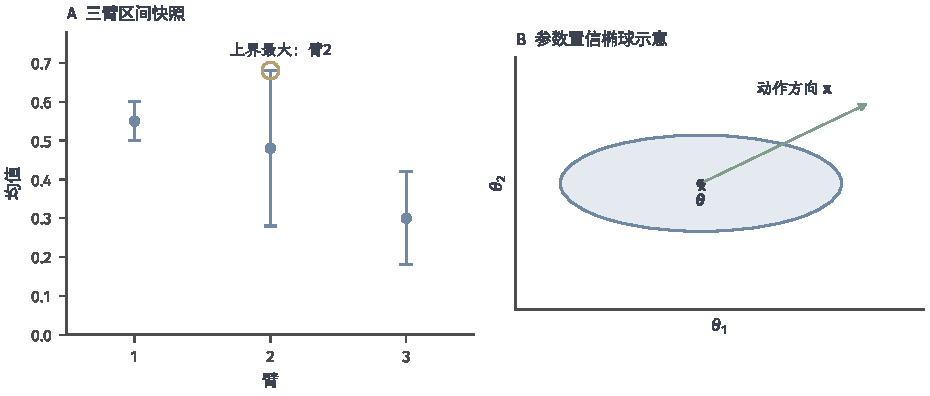
\includegraphics[width=157.400mm]{figures/10-reinforcement-learning/01-problems-and-solving/matplotlib/rl-learning-bandit-geometry.pdf}
  \caption{动作区间与参数椭球。左图为明确标注的三臂教学快照，UCB选择上端点最大的第二臂；右图示意线性参数置信集合，较长的轴对应奖励样本约束较弱的参数方向。二者都把不确定性转成动作评分，但线性模型还通过共享特征把奖励样本的约束扩展到其他动作。}
  \label{fig:rl-learning-bandit-geometry}
\end{figure*}

\Needspace{14\baselineskip}
LinUCB常以这个方向性奖励构造动作评分；OFUL直接在联合参数置信集合中做乐观选择，并把集合有效性纳入分析\scite{rl3-abbasi2011linear}
线性Thompson采样则抽取整个参数向量，再对所有动作用同一个抽样参数评分。共享的是线性结构和设计矩阵，而不是“把标量UCB换成更大网络”就能保留的保证。具体统计结论依赖所用噪声模型、置信半径或抽样尺度。

若奖励规律不固定，每个臂可能根本没有待估计的固定均值。我们改用无上下文的对抗老虎机：对手在本轮实际抽样前选择奖励向量$\bm{r}_t\in[0,1]^K$，智能体只看到$r_{t,a_t}$。对手可依赖过去历史，却不能在看到本轮动作后临时改写奖励。此时EXP3用权重记录各臂迄今的奖励证据，并把权重归一化成抽样概率。为更新未被选臂也有定义的奖励估计，所选臂的奖励除以其抽样概率，其他臂记0；下面三式依次给出抽样、估计与指数权重更新：
\begin{equation}
  p_{t,a}=(1-\varepsilon)\frac{w_{t,a}}{\sum_b w_{t,b}}
                 +\frac{\varepsilon}{K},\quad
  \widehat r_{t,a}=\frac{\mathbf 1\{a_t=a\}r_{t,a_t}}{p_{t,a}},
  \quad
  w_{t+1,a}=w_{t,a}\exp(\eta\widehat r_{t,a})
  \label{eq:rl-learning-exp3}
\end{equation}
估计奖励较高的臂获得更大的下一轮权重。各臂权重从正值开始；$0<\varepsilon\leq1$保证所有抽样概率为正，$\eta$与$\varepsilon$必须按具体遗憾分析配合，而不能任意取大值。

逆概率加权的意义可以先用一个数看清。固定某轮奖励为$0.6$的臂，若它以概率$0.2$被选中，就在选中时记$0.6/0.2=3$，其余时候记0。平均为$0.2\times3=0.6$，恰好恢复该臂本轮奖励。这个估计数可以超过奖励上限1，因为它承担的是补偿少抽样的权重，不是模拟一次真实奖励。抽样概率越小，偶尔出现的加权值越大，有限样本波动也越强。

无偏性的条件可以直接检查。固定抽样前历史及本轮奖励向量后，
\[
  \mathbb E[\widehat r_{t,a}\mid\text{历史},\bm{r}_t]
  =p_{t,a}\frac{r_{t,a}}{p_{t,a}}=r_{t,a}.
\]
概率小会放大方差，但不会在这些条件下改变条件均值。若对手看到$a_t$后才选择$\bm{r}_t$，这一步条件化便不成立。通常的外部遗憾比较事后最佳固定臂，而不是每轮都预知奖励的全知动作序列；对抗上下文算法还要明确比较的策略类。EXP3的原始保证正是围绕这种反馈与比较协议建立的\scite{rl3-auer2002nonstochastic}

% Outline: 3.1.4
\subsection{学习目标变化：累积遗憾与最佳臂识别}
\label{sec:rl-learning-best-arm}

同样的随机老虎机，若试验期间也要服务用户，就需要控制累积收益损失；若只在试验后部署一个动作，则可以多试当前看来略差的候选，换取更可靠的推荐。后一种任务称为最佳臂识别，评价的是输出而非整段动作序列。预算结束时输出$\widehat a_T$，下面分别计算它比最佳均值差多少，以及它落在最优臂集合之外的概率；两者都越小越好：
\begin{equation}
  \mathfrak r_T=\mathbb E[m_*-m_{\widehat a_T}],
  \qquad
  \mathbb P\{\widehat a_T\notin\argmax_a m_a\}.
  \label{eq:rl-learning-simple-regret}
\end{equation}
错选一个只差$10^{-4}$的动作，对这两个指标的影响并不相同。仅报告推荐错误率会把近乎无损与严重失误放在同一类别中。表\ref{tab:rl-learning-identification-protocols}进一步区分何时结束试验：预算耗尽与证据充分，是两种不同的停止依据。

\begin{table}[htbp]
  \centering
  \small
  \begin{tabularx}{\linewidth}{>{\raggedright\arraybackslash}p{22mm} >{\raggedright\arraybackslash}X >{\raggedright\arraybackslash}X}
    \toprule
    协议 & 预先固定什么 & 算法输出与待分析量 \\
    \midrule
    固定预算 & 总拉臂次数$T$ & 推荐$\widehat a_T$；分析简单遗憾或错误概率 \\
    固定置信度 & 允许错误$\delta$，必要时精度$\epsilon$ & 随机停止时间$\tau$和推荐$\widehat a_\tau$；保证错误概率不超过$\delta$并分析$\mathbb E\tau$ \\
    \bottomrule
  \end{tabularx}
  \caption{纯探索的两种协议。固定置信度不是先任意选择预算，再宣称置信度已经满足。}
  \label{tab:rl-learning-identification-protocols}
\end{table}

固定置信度协议允许边采样边检查是否停止，因而停止时的样本数由已见奖励记录决定。只在某个预先固定样本数有效的区间不足以支持这种反复查看。我们给全部臂、全部正整数样本数同时分配失覆盖概率；对$[0,1]$奖励，取下面的半宽与区间：
\[
  \begin{aligned}
    c(n)&=\sqrt{\frac{\log(2K n(n+1)/\delta)}{2n}},\\
    [L_a(n),U_a(n)]&=[\widehat m_a(n)-c(n),\widehat m_a(n)+c(n)].
  \end{aligned}
\]
Hoeffding不等式给出单个$(a,n)$的失覆盖概率不超过$\delta/[K n(n+1)]$。因为$\sum_{n\geq1}1/[n(n+1)]=1$，联合界保证全部臂、全部样本数同时覆盖的概率至少为$1-\delta$。这不是最紧的边界，却明确处理了自适应停止。

\term{逐次淘汰}（successive elimination）保留尚可能最优的臂；若$U_a<\max_b L_b$，则淘汰$a$。在全部区间覆盖的事件上，真正最优臂不可能满足淘汰条件。教学快照若三个区间为$[0.55,0.65]$、$[0.40,0.52]$、$[0.42,0.70]$，第二臂可淘汰，第一、第三臂还不能分胜负。LUCB把试验集中到当前经验最优臂$b$与其余臂中上界最大的竞争者$c$\scite{rl3-kalyanakrishnan2012pac}
当$L_b\geq U_c-\epsilon$时，可以推荐一个$\epsilon$-最优臂。这个例子中下一步重点采第一和第三臂，而不是轮流采已排除的第二臂。

区间正确时，淘汰和停止逻辑便给出正确性；样本复杂度还要分析何时区间足够窄。固定置信度理论进一步研究不同臂之间的最优样本分配\scite{rl3-kaufmann2016complexity}
从区间宽度看，为了分开差距$\Delta_a$，半宽通常要降到$\Delta_a$的常数比例，所需样本因而带有$\Delta_a^{-2}$量级和置信度对数项，但这一粗略尺度不能给出最优常数。差距趋近0会使精确识别越来越昂贵；并列最优时，要求用严格区间分离证明唯一最优可能永不停止，应改用适合并列情形的识别目标，例如允许正精度的$\epsilon$-最优识别。

% Outline: 3.1.5
\subsection{状态随动作变化：MDP中的覆盖、可达性与长时程探索}
\label{sec:rl-learning-deep-exploration}

回到MDP，每轮并不会自动把智能体送回同一组候选动作面前。某扇门只有到达门口才能尝试，一次转向可能让后续奖励区域暂时不可达。图\ref{fig:rl-learning-exploration-chain}左侧是由网格导航抽出的独立教学链：取消滑移，增设单向门与失败后重置，连续$H$次必要选择才能到达唯一奖励。若每次独立均匀试两个动作，一回合走完全链的概率为$2^{-H}$；这个数字描述该随机试验方案，不是所有能观察状态的算法都必须付出的下界。

\begin{figure*}[t]
  \centering
  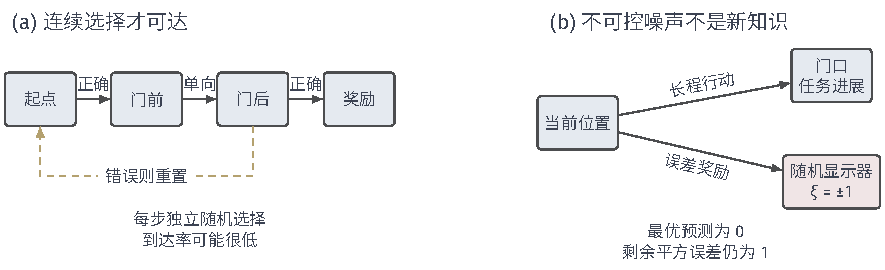
\includegraphics[width=149.818mm]{figures/10-reinforcement-learning/01-problems-and-solving/tikz/rl-learning-exploration-chain.pdf}
  \caption{可达性与预测误差的两个教学反例。左侧为从导航任务抽出的确定性单向门链，每一步错误都会重置；右侧的随机显示器可持续制造不可控预测误差，却不帮助通过门口。两者均为明确修改过的独立任务，不是基准网格的新转移规则。}
  \label{fig:rl-learning-exploration-chain}
\end{figure*}

在这条链上，“试一下最后一道门”首先要求走过前面的门。已经确认的前缀应被后续探索保留，新的随机选择集中在尚不了解的部分。这样的长时程探索将一次试验看成持续多步的行为：当前动作不仅为了本步奖励，也为了取得较远处的证据。下面的乐观备份和整回合后验采样，分别用价值传播和一致的模型假设维持这种方向。

要探索链末端，当前动作必须能利用对远处尚未确定收益的估计。乐观价值先给未充分访问的状态动作较高估值，再通过Bellman备份将它传向上游；模型置信集合则保留尚未被已见转移与奖励记录排除的转移核与奖励规律，选其中预计回报较高的模型来规划。后验采样强化学习（posterior sampling for reinforcement learning, PSRL）在回合开始抽取一套完整动力学和奖励，再在整回合执行其策略。这样多个时刻共享同一个探索假设，不会像逐步重新随机选方向那样频繁放弃当前路线。后验及其计算仍依赖模型假设，有限样本表格保证将在第\ref{sec:rl-learning-statistical-limits}节另列条件\scite{rl3-osband2013posterior}

也可以不显式规划一个乐观模型，而在训练奖励中加入鼓励访问未充分采样状态动作的内部信号。这称为内在奖励（intrinsic reward）：外在任务奖励仍为$r_t$，训练使用$r_t+\eta_{\mathrm{int}} b_t$，其中$b_t$由采样或预测记录构造，$\eta_{\mathrm{int}}$决定探索信号的权重。表\ref{tab:rl-learning-intrinsic}比较不同$b_t$的测量对象。加入它会改变训练时的选择偏好，所以评价必须另报不含内在奖励的任务回报，才能确认探索最终帮助了原任务。

用预测误差产生内在奖励时，需要先明确“预测什么”。ICM（intrinsic curiosity module，内在好奇心模块）用当前与后继特征反推已执行动作，借此训练表示，再预测给定动作后的特征；预测错的部分产生内部奖励。RND（random network distillation，随机网络蒸馏）则固定一个随机初始化的网络，用另一个网络模仿它对当前观测的输出。观测越少参与拟合，输出差可能越大；固定目标网络并不是在预测真实环境。两者都把某种拟合误差转为探索信号，是否测到可减少的无知，还要检查噪声和表示。

\begin{table*}[t]
  \centering
  \small
  \begin{tabularx}{\linewidth}{>{\raggedright\arraybackslash}p{24mm} >{\raggedright\arraybackslash}X >{\raggedright\arraybackslash}X}
    \toprule
    方法 & 估计对象与典型信号 & 怎样改变行为及主要边界 \\
    \midrule
    访问计数 & $b_t(s,a)=1/\sqrt{N_t(s,a)+1}$ & 奖励少访问位置；离散计数需要有意义的状态划分 \\
    伪计数 & 用密度模型更新前后的概率变化构造计数替代 & 将新颖性扩到大状态空间；依赖密度学习假设，不是实际访问次数 \\
    ICM & 学习特征中的动作条件前向预测误差，配合逆动力学表示 & 偏向可由动作影响的特征；不能保证剔除所有噪声 \\
    RND & 可训练预测器与固定随机目标网络的输出差 & 以拟合困难代表新颖性；泛化、遗忘和观测噪声会影响分数 \\
    回合内好奇心 & 当前嵌入与本回合记忆的距离或近邻密度 & 鼓励回合内未访区域；跨回合重置记忆改变了“新”的含义 \\
    \bottomrule
  \end{tabularx}
  \caption{新颖性信号的计算对象。表中的奖励是训练工具，不自动对应环境转移的置信区间。}
  \label{tab:rl-learning-intrinsic}
\end{table*}

按表中的计数公式，同一教学状态的两个动作已访问99次和3次，探索奖励分别为$0.1$和$0.5$；后者因样本更少而得到更高偏好。预测误差却可能在观测样本充分后仍然很大。设与位置无关的显示器每步独立输出$\xi_t\in\{-1,1\}$，两值等概率。平方损失下最优预测为0，剩余期望误差仍是$\mathbb E\xi_t^2=1$。把这项误差奖励给智能体，可能使它停在显示器旁：它已经知道显示规律，却仍能持续获取探索奖励。这就是noisy-TV反例，说明不可预测性不能直接当成可通过采样减少的无知。

\Needspace{16\baselineskip}
ICM在学习到的特征空间预测动作后果，用预测误差提供探索信号；表示的学习目标影响哪些变化会被当成值得探索的后果\scite{rl3-pathak2017curiosity}

\Needspace{16\baselineskip}
RND改为预测固定随机网络的输出，避免直接用随机后继的不可预测性作为目标；但其新颖性仍依赖观测表示、预测器训练及其训练观测样本的分布\scite{rl3-burda2019rnd}
ICM、RND与回合记忆分别改变表示、预测目标或比较范围，缓解条件并不相同。

在特别稀疏的任务中，还要区分“发现过某个状态”与“能稳定再到达它”。Go-Explore保存已发现状态及其到达路径，返回选定状态后继续探索，再处理带执行随机性的稳健复现。模拟器存档恢复提供了普通单轨迹交互没有的访问能力；即使两者都记录一百万步，允许采集的状态动作与重置条件也不同。探索性课程可以从更易到达的起点或子目标逐步扩展，但必须说明谁提供重置和任务选择。目标重标记如何把失败轨迹变成其他任务的成功经验，留到第\ref{chap:rl-transfer}章讨论\scite{rl3-ecoffet2021goexplore}

若勘查时还不知道将来要送往哪一个区域，探索目标就不能只围绕当前任务奖励。奖励无关探索先收集转移记录，奖励函数在采集结束后才给出，要求不再交互也能为它规划。此时重要的是记录能否支持全部允许奖励下的决策，而非已有技能是否容易区分；具体协议与统一保证见第\ref{sec:rl-learning-guarantees-access}节。

% Outline: 3.2
\section{无模型的价值学习}
\label{sec:rl-learning-value}

取得经验后，还需把观察到的奖励和后继变成长期价值估计。第\ref{chap:rl-planning}章的Bellman备份计算条件期望；现在只能用样本逼近它。固定产生目标回报的策略后，完整回报与自举目标具有不同的采样和估计误差；根据价值进一步改变行为或共享函数参数，又会引入评价与改进的耦合。

% Outline: 3.2.1
\subsection{完整回报与一步自举}
\label{sec:rl-learning-mc-td}

一条到达终点的轨迹已记录沿途全部奖励，我们可以把某次访问之后的奖励折扣相加，作为该状态的一次价值样本。\term{蒙特卡罗}（Monte Carlo, MC）评价就用这种完整随机回报修正估值：样本回报高于当前预测时上调，低于预测时下调。设回合在$T$终止，$V(s_T)=0$，目标及更新为
\begin{equation}
  G_t=\sum_{j=0}^{T-t-1}\gamma^j r_{t+j},
  \qquad
  V(s_t)\leftarrow V(s_t)+\alpha_t[G_t-V(s_t)].
  \label{eq:rl-learning-mc}
\end{equation}
更新中的$\alpha_t$是步长，控制这次样本占多大权重。把第二式写成$(1-\alpha_t)V(s_t)+\alpha_tG_t$，就能看出它在旧估计与新回报之间加权。若某状态已有$n-1$个选定回报样本的均值，第$n$个样本到来时取$\alpha=1/n$，更新后恰为$n$个样本的均值。因此这条递推首先是一种不必保存全部旧回报的平均算法；其他步长则采用不同加权，不能都解释成普通样本均值。

首次访问MC对每回合第一次出现的状态更新，每次访问MC对该状态的所有出现都更新。二者利用的回报都来自真实奖励，但同一回合内重复访问对应的回报并不独立。

若回合很长，等待完整回报会推迟更新；继续任务甚至没有自然的回合终点。Bellman关系提供了另一种目标：把已观察的一步奖励与下一状态的当前估值相加。\term{时序差分}（temporal difference, TD）用这个目标与当前预测的差立即更新，$\delta_t$就是这次样本的预测差：
\begin{equation}
  \delta_t=r_t+\gamma V(s_{t+1})-V(s_t),\qquad
  V(s_t)\leftarrow V(s_t)+\alpha_t\delta_t .
  \label{eq:rl-learning-td-zero}
\end{equation}
这种用已有预测构造新目标的做法称为\term{自举}（bootstrapping）。终止转移的下一价值是0；继续任务的人工时间截断则不能一概置0。表\ref{tab:rl-learning-mc-td}把目标的偏差来源与更新时机分开，避免把一步目标尚不准确误解为最终估计必然有偏。

\begin{example}[同一终止轨迹上的不同目标]
  \label{ex:rl-learning-mc-td}
  在基准随机网格中，一条可能的轨迹依次经过
  \[
    (1,1),(1,1),(2,1),(3,1),(4,1),(4,2),(4,3).
  \]
  第一次向右时向下滑移撞墙，因此留在原位；其后五步实现意图方向。奖励为五个$-0.04$和末步的1。于是起点两次访问的回报分别为
  \[
    \begin{aligned}
      G_0&=-0.04\frac{1-0.9^5}{1-0.9}+0.9^5=0.426686,\\
      G_1&=-0.04\frac{1-0.9^4}{1-0.9}+0.9^4=0.51854.
    \end{aligned}
  \]
  只看这一回合，首次访问样本是$0.426686$，每次访问的样本平均为$0.472613$。它们都是该轨迹产生的估计，不是起点的精确策略价值。若冻结估值$V(1,1)=0.2$、$V(2,1)=0.3$，前两次TD目标却分别是$-0.04+0.9(0.2)=0.14$和$-0.04+0.9(0.3)=0.23$。取步长$0.5$，第一条TD更新把起点估值从$0.2$改为$0.17$；从相同初值做首次访问MC则得到$0.313343$。这里为了比较目标没有把各方法串行混用。
\end{example}

\begin{table}[htbp]
  \centering
  \small
  \begin{tabularx}{\linewidth}{>{\raggedright\arraybackslash}p{22mm} >{\raggedright\arraybackslash}X >{\raggedright\arraybackslash}X}
    \toprule
    比较对象 & MC & TD(0) \\
    \midrule
    更新何时可得 & 等实际回报完成 & 观察一步转移即可 \\
    随机性来源 & 之后整段奖励和状态 & 当步奖励、后继状态及当前估值 \\
    对初值的依赖 & 初值不进入回报目标 & 后继估值进入目标 \\
    目标的条件均值 & 固定策略完整回报对应$V^\pi$ & 对应$\mathcal B^\pi V$，通常不等于$V^\pi$ \\
    适用注意 & 需终止或处理无限回报尾项 & 需控制自举与采样条件 \\
    \bottomrule
  \end{tabularx}
  \caption{目标偏差不等于最终估计偏差。TD目标含当前估值，不妨碍满足条件的表格迭代最终收敛到真实价值。}
  \label{tab:rl-learning-mc-td}
\end{table}

MC以已实现的整段回报作为目标，TD则把未来分成“刚看到的一步”和“尚未看到的其余部分”。后一部分由$V(s_{t+1})$暂时代替，所以目标会随价值估计一起改变。若后继估值过高，当前状态也可能被上调；若后继估值逐渐纠正，误差又会沿访问过程传回来。TD(0)中的0表示这里不使用跨步资格迹，资格迹将在下一小节解释。

随机的一步目标不必每次都更接近真实价值。固定当前估值$V$，对从状态$s$出发按$\pi$得到的许多一步样本平均，平均目标才是前章的$(\mathcal B^\pi V)(s)$。这里$\mathcal B^\pi$仍表示“即时奖励均值加折扣后继价值均值”。TD要用带噪声的更新追踪这项平均备份，直至备份前后相同；这与拿一个已知的正确标签做回归不同。

固定策略时，对给定$s_t=s$的动作、奖励和后继取平均，TD误差的条件均值为$(\mathcal B^\pi V)(s)-V(s)$。因此，样本更新虽然有噪声，平均方向仍指向Bellman不动点。在有限折扣MDP中，若奖励二阶矩受控、策略固定、每个需要评价的状态被无限访问，且各状态的访问步长满足$\sum_n\alpha_n(s)=\infty$、$\sum_n\alpha_n(s)^2<\infty$，配合相应马尔可夫噪声条件，可用随机逼近证明表格TD收敛。步长和发散使初始误差有机会被持续修正，平方和收敛则限制噪声的长期影响；Bellman压缩性确定唯一平衡点。这不覆盖任意常数步长或任意函数逼近。

MC的一致性则直接来自回报平均：独立回合的首次访问回报可用大数定律，每次访问版本要处理回合内依赖和访问次数的随机性。无限时域折扣MC若只截取有限长度，还留下尾项偏差。MC与TD都依赖轨迹采集和抽样条件，但依赖的方式不同\scite{sutton2018}

% Outline: 3.2.2
\subsection{多步回报、资格迹与时间信用}
\label{sec:rl-learning-traces}

MC一直使用真实奖励直到终点，TD(0)在一步之后就接入预测。若奖励需要多步才能传回当前状态，可以先观察$n$步奖励，再用第$n$步的估值补上余下未来。对固定估值$V$和终止时刻$T$，令$m=T-t$，允许长度$1\leq n\leq m$，得到
\begin{equation}
  G_t^{[n]}=\sum_{j=0}^{n-1}\gamma^j r_{t+j}
                    +\gamma^n V(s_{t+n}),\qquad V(s_T)=0.
  \label{eq:rl-learning-n-step}
\end{equation}
方括号$[n]$表示目标长度，不是参数迭代。$n$增大让奖励影响更快传过多步，但也把更多未来随机性带入一次目标。

先作一个独立的三步终止算例，观察目标长度改变了哪一部分。设奖励依次为$0,0,1$，$\gamma=0.9$，当前后继估值为$V(s_1)=0.2,V(s_2)=0.5,V(s_3)=0$。起点的一步、两步和完整三步目标分别是$0.18,0.405,0.81$。一步目标只读取$s_1$的预测，三步目标已读到真实终点奖励。这里数值差来自指定初值，不表示较长目标每次都更准；一般任务中多读真实奖励，也会多承受后续随机性。

\term{$\lambda$回报}（lambda return）用一组几何权重混合这些长度，不再只选一个$n$。参数$\lambda$越大，越多权重交给较长的真实奖励段。对$0\leq\lambda\leq1$，混合目标为
\begin{equation}
  G_t^\lambda
    =(1-\lambda)\sum_{n=1}^{m-1}\lambda^{n-1}G_t^{[n]}
                     +\lambda^{m-1}G_t^{[m]} .
  \label{eq:rl-learning-lambda-return}
\end{equation}
末项收走所有剩余权重，故权重之和为1；$\lambda=0$得到一步目标，$\lambda=1$得到完整回报。若采样片段只是截断而非终止，末端$V$必须保留。

仍用三步算例，取$\lambda=0.5$时，三个长度的权重依次为$0.5,0.25,0.25$，所以$G_0^\lambda=0.5(0.18)+0.25(0.405)+0.25(0.81)=0.39375$。较早结束的目标占一部分，剩余权重继续交给较长目标，直到末项全部收走。这解释了末项为何不能再乘$1-\lambda$：否则混合权重之和会小于1。

上述计算从一次访问出发，把后续奖励组合成它的更新目标，称为前向视图。完整的$\lambda$回报需要等到后续奖励出现才能算出。若希望每收到一个TD误差就立即利用它，可以反过来保存过去访问的影响：每次访问加入当前价值对参数的梯度，旧的梯度贡献则逐步衰减。这份累积记录称为\term{资格迹}（eligibility trace）；当前TD误差乘以资格迹，就能同时修正与过去访问有关的参数，这称为后向视图。下面在有限终止轨迹上冻结参数，证明两种方式累计的更新相同。比较截断片段上的前后向计算时，也必须采用相同的末端自举值。

在表格表示中，价值参数就是各状态的表项，$\nabla V(s)$是一份只在当前状态分量为1、其余为0的记录。资格迹先给当前状态记1，再让过去记录乘$\gamma\lambda$衰减。若奖励到达时刚才几个状态的迹还非零，一个TD误差就能同时更新这些表项；在线性表示中，把这份单状态记录换成特征向量即可。这样把“未来奖励应影响哪些过去判断”变成可维护的记录，就是时间信用分配在这里的含义。接下来的证明核对前后两种计算在固定参数时是否累计了同一批影响。

\begin{theorem}[固定参数下前后向更新等价]
  \label{thm:rl-learning-trace-equivalence}
  设$T\geq1$为整数，$0\leq\gamma\leq1$、$0\leq\lambda\leq1$。给定终止轨迹$(s_0,r_0,\ldots,s_{T-1},r_{T-1},s_T)$，固定可微状态价值函数$V_{\bm\theta}$及参数$\bm\theta$，并令$V_{\bm\theta}(s_T)=0$。用式\eqref{eq:rl-learning-n-step}与式\eqref{eq:rl-learning-lambda-return}定义各步的$G_t^{[n]}$和$G_t^\lambda$。定义$\delta_k=r_k+\gamma V_{\bm\theta}(s_{k+1})-V_{\bm\theta}(s_k)$。从$\bm e_{-1}=\bm0$递推积累资格迹
  \[
    \bm{e}_k=\gamma\lambda\bm{e}_{k-1}
                    +\nabla_{\bm{\theta}}V_{\bm{\theta}}(s_k).
  \]
  若整回合结束后一次性应用更新，则
  \begin{equation}
    \sum_{t=0}^{T-1}
      (G_t^\lambda-V_{\bm{\theta}}(s_t))
      \nabla_{\bm{\theta}}V_{\bm{\theta}}(s_t)
      =\sum_{k=0}^{T-1}\delta_k\bm{e}_k .
    \label{eq:rl-learning-trace-equivalence}
  \end{equation}
\end{theorem}
\begin{proof}
  先对$n$步目标作望远镜展开：
  \[
    G_t^{[n]}-V(s_t)
       =\sum_{j=0}^{n-1}\gamma^j
          [r_{t+j}+\gamma V(s_{t+j+1})-V(s_{t+j})]
       =\sum_{j=0}^{n-1}\gamma^j\delta_{t+j}.
  \]
  在式\eqref{eq:rl-learning-lambda-return}中，$\delta_{t+j}$出现在所有$n\geq j+1$的项内。它的总系数为
  \[
    \gamma^j\left[(1-\lambda)
       \sum_{n=j+1}^{m-1}\lambda^{n-1}
       +\lambda^{m-1}\right]=(\gamma\lambda)^j.
  \]
  端点$\lambda=0,1$可直接代入定义验证。因此
  $G_t^\lambda-V(s_t)=\sum_{k=t}^{T-1}(\gamma\lambda)^{k-t}\delta_k$。
  交换有限和得到
  \[
    \sum_{t=0}^{T-1}\sum_{k=t}^{T-1}
       (\gamma\lambda)^{k-t}\delta_k\nabla V(s_t)
    =
    \sum_{k=0}^{T-1}\delta_k
       \sum_{t=0}^k(\gamma\lambda)^{k-t}\nabla V(s_t).
  \]
  内层和正是递推定义的$\bm{e}_k$，故两种总更新相同。
\end{proof}

若$\gamma=0.9$、$\lambda=0.8$，资格迹对当前、前一次和前两次访问的梯度贡献分别赋予权重$1,0.72,0.5184$，见图\ref{fig:rl-learning-traces}。当前误差因而可以影响较早的预测，无须等待回合结束。但上一定理的等价性限定了固定参数；每步更新参数后，过去目标和梯度都可能改变。表\ref{tab:rl-learning-trace-variants}据此区分改变迹、修正在线更新和重分配奖励三类操作。

\begin{figure}[htbp]
  \centering
  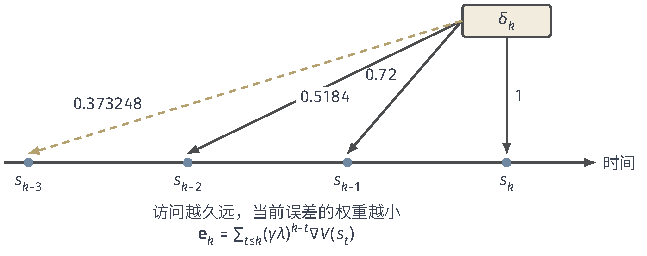
\includegraphics[width=109.583mm]{figures/10-reinforcement-learning/01-problems-and-solving/tikz/rl-learning-traces.pdf}
  \caption{同一个TD误差的后向信用分配。横轴为访问时刻，箭头上的数值来自$\gamma\lambda=0.72$。前向视图把未来误差加给当前状态，后向视图在误差出现时按资格迹更新与过去访问有关的参数。}
  \label{fig:rl-learning-traces}
\end{figure}

\begin{table*}[t]
  \centering
  \small
  \begin{tabularx}{\linewidth}{>{\raggedright\arraybackslash}p{26mm} >{\raggedright\arraybackslash}X >{\raggedright\arraybackslash}X}
    \toprule
    方法 & 改变什么 & 需要保留的边界 \\
    \midrule
    积累迹 & 每次访问都加上特征，旧迹乘$\gamma\lambda$ & 重复访问会累加；等价定理使用固定参数 \\
    替换迹 & 表格或二值特征中，把本次激活分量置1而非继续累加 & 改变重复访问权重；一般稠密特征不能照搬“置1”语义 \\
    真实在线TD & 使用修正的迹与更新，匹配随时间变化的前向目标 & 经典精确等价针对线性表示的在线前向视图，不是任意网络的代数恒等式 \\
    奖励重分配 & 把延迟奖励分配到预测中关键的过去事件 & 保持目标须保证逐轨迹折扣总和相等，或明确等价条件 \\
    \bottomrule
  \end{tabularx}
  \caption{改变信用传播与改变奖励位置并非同一操作。真实在线TD修正参数变化引起的偏差，RUDDER类方法则学习奖励应归到哪些事件。}
  \label{tab:rl-learning-trace-variants}
\end{table*}

真实在线TD的修正正是为了让在线参数变化也有明确的前向解释\scite{rl3-vanseijen2014true}

\Needspace{14\baselineskip}
RUDDER利用序列回报预测，把预测变化归给较早的关键事件\scite{rl3-arjona2019rudder}
在有限回合、未折扣回报下，重分配若满足$\sum_t\widetilde r_t=\sum_t r_t$，就保留逐轨迹总回报；折扣目标则需要$\sum_t\gamma^t\widetilde r_t=\sum_t\gamma^t r_t$，不能只核对未加权总和。预测不完整时还要有残差补偿或另外分析误差。即使奖励位置改得很合适，从未到达过奖励区域的转移与奖励记录也不能凭空告诉模型那里有什么。

% Outline: 3.2.3
\subsection{离策略回报估计与校正}
\label{sec:rl-learning-off-policy}

策略改进后，回放中的旧轨迹仍可利用，但直接平均其回报会评价采集这些轨迹记录的旧策略，而非当前目标策略。我们将前者称为行为策略$\beta$，后者称为目标策略$\pi$。两者共享环境时，轨迹概率的差别来自动作抽样；重要性校正按这一概率比重新加权，使行为策略采集的轨迹记录可用于目标策略评价。前提是目标可能产生的轨迹在行为分布下也有机会出现，否则任何权重都无法补出缺失经验。

先看只有一个决策的教学例。行为策略以概率$1/2$选右，目标策略以概率$0.8$选右。对于“选右后收到奖励”的记录，权重为$0.8/(1/2)=1.6$；对于选左记录，权重为$0.2/(1/2)=0.4$。于是行为抽样后的平均加权回报为$0.8$倍右动作奖励均值加$0.2$倍左动作奖励均值，正好等于目标策略回报。这就是重要性采样（importance sampling）：样本仍来自原分布，但通过权重计算另一分布的期望。

连续多步时，一条动作前缀在目标策略下的概率是各步目标动作概率的乘积，行为策略下同样如此，所以校正权重也相乘。已经发生的$r_t$只需要截至动作$t$的前缀权重，后来的动作不改变这项奖励。定理将这个直觉写成完整轨迹与逐决策两种公式；其中“目标律绝对连续于行为律”正是前述要求，即行为分布不能给目标可能出现的事件零概率。

\begin{theorem}[轨迹与逐决策重要性校正]
  \label{thm:rl-learning-importance-sampling}
  设$H\geq1$为整数，$0\leq\gamma\leq1$，状态与合法动作集有限。固定平稳Markov行为策略$\beta$与目标策略$\pi$，二者使用同一初始分布$\mu_0$及同一联合奖励转移核$p(\mathrm dr,s'\mid s,a)$。令$G_0=\sum_{t=0}^{H-1}\gamma^t r_t$。设目标轨迹律$P_{\mathcal E}^{\pi}$绝对连续于行为轨迹律$P_{\mathcal E}^{\beta}$，且对各$t<H$有$\mathbb E_\pi|r_t|<\infty$。在行为实际产生的历史上记
  \[
    \rho_t=\frac{\pi(a_t\mid s_t)}{\beta(a_t\mid s_t)},\qquad
    W_{u:v}=\prod_{k=u}^{v}\rho_k .
  \]
  则
  \begin{equation}
    \mathbb E_\pi G_0
       =\mathbb E_\beta[W_{0:H-1}G_0]
       =\mathbb E_\beta\left[\sum_{t=0}^{H-1}
                           \gamma^t W_{0:t}r_t\right].
    \label{eq:rl-learning-is}
  \end{equation}
\end{theorem}
\begin{proof}
  对轨迹$\tau=(s_0,a_0,r_0,\ldots,s_H)$，共同初始分布和联合奖励转移核给出按发生顺序的测度乘积
  \[
    P_{\mathcal E}^{\pi}(\mathrm d\tau)
      =\mu_0(s_0)\prod_{t=0}^{H-1}
        \pi(a_t\mid s_t)\,p(\mathrm dr_t,s_{t+1}\mid s_t,a_t).
  \]
  Radon--Nikodym导数在行为轨迹律几乎处处意义下为$W_{0:H-1}$。行为概率为0的历史可任意约定权重版本，例如取0；绝对连续性保证不会遗漏目标质量。对可积回报应用换测度，得到第一个等式。

  再把轨迹截到$r_t,s_{t+1}$，记此前缀为$\tau_{0:t+1}$。对剩余轨迹积分后，两条策略的前缀分布仍由相同环境核与各自动作概率相乘得到，故前缀密度比为$W_{0:t}$。完整轨迹的绝对连续性也保证前缀绝对连续。将换测度分别用于非负的$|r_t|$，得到
  \[
    \mathbb E_\beta[W_{0:H-1}|r_t|]
    =\mathbb E_\beta[W_{0:t}|r_t|]
    =\mathbb E_\pi|r_t|<\infty.
  \]
  因而下面各项期望均存在。由于$r_t$仅依赖该前缀，
  \[
    \mathbb E_\beta[W_{0:H-1}r_t]
    =\mathbb E_\pi[r_t]
    =\mathbb E_\beta[W_{0:t}r_t].
  \]
  对有限个奖励项加权求和，得到逐决策形式。这个前缀论证不要求在目标概率为0的行为历史上，未来概率比也具有条件均值1。
\end{proof}

以网格中一段两步动作前缀为例，若行为动作概率分别为$1/2,1/4$，目标概率分别为$0.8,0.6$，则比率为$1.6,2.4$，乘积为$3.84$。对应奖励对逐决策估计的贡献为$1.6r_0+0.9(3.84)r_1$。概率比不含滑移概率，因为两条策略共享同一转移核；若这些轨迹记录由另一种滑移机制生成，这个消去理由便不存在。

方差问题在最简单的教学模型中就会出现：目标策略必选的两步动作，在行为策略下每步概率都是0.1，故该前缀仅以0.01发生，权重为100。设仅成功前缀末端奖励为1，其余为0且暂取$\gamma=1$，无偏估计量以概率0.01取100，否则取0，均值为1而方差为99。图\ref{fig:rl-learning-is-sampling}把低概率和大权重画在同一条路径上。若行为概率改成0，权重技巧就完全失效。

\begin{figure}[htbp]
  \centering
  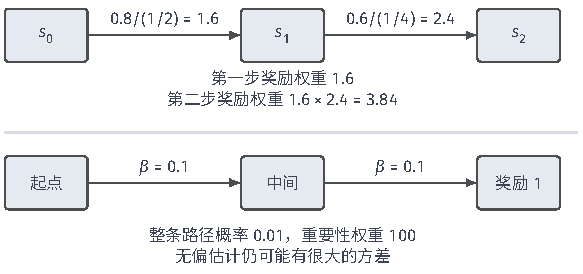
\includegraphics[width=98.651mm]{figures/10-reinforcement-learning/01-problems-and-solving/tikz/rl-learning-is-sampling.pdf}
  \caption{两步重要性权重的乘积。上方为可手算的网格动作前缀，下方为独立的罕见路径教学例；共同环境核不进入比率。宽支持是可校正的前提，大权重则是方差问题。}
  \label{fig:rl-learning-is-sampling}
\end{figure}

直接将过大的总权重截小，会连期望一并改变。在上面的罕见路径例中，若把权重100截为10，平均估计从1降到$0.01\times10=0.1$。要在控制波动时仍评价指定策略，就必须设计不同的误差传播方式或补偿项；下面的多步方法需要分清截断的是当前奖励权重，还是未来误差传回来的系数。

完整概率比积可能随时域增长而剧烈波动。多步自举可以改为传播逐步Bellman误差，并限制较远误差的权重，但是否保留目标策略取决于截断位置。先固定$\pi$，在后继状态对其合法动作按概率求平均，构造
\[
  \delta_t^\pi=r_t+\gamma\sum_a\pi(a\mid s_{t+1})Q(s_{t+1},a)
                       -Q(s_t,a_t).
\]
Retrace使用$c_t=\lambda\min(1,\rho_t)$，从给定$(s_t,a_t)$构造
\begin{equation}
  Q_{\mathrm{ret},t}
   =Q(s_t,a_t)+\sum_{k=t}^{T-1}
        \gamma^{k-t}\left(\prod_{j=t+1}^{k}c_j\right)\delta_k^\pi .
  \label{eq:rl-learning-retrace}
\end{equation}
空积为1。注意第一项误差不乘$\rho_t$，因为这里评价的起始动作已给定；$\pi$期望进入每个Bellman误差，截断系数只控制更远误差的传播。教学例若$\delta_t^\pi=0.4$、$\delta_{t+1}^\pi=-0.2$、$\lambda=0.8$、$\rho_{t+1}=2$，则增量为$0.4+0.9(0.8)(-0.2)=0.256$。以步长$0.5$更新时，起始$Q$增加$0.128$。表\ref{tab:rl-learning-off-policy-targets}比较不同方法的截断位置，尤其要看当前误差与后续迹是否承担不同权重。

\begin{table*}[t]
  \centering
  \small
  \begin{tabularx}{\linewidth}{>{\raggedright\arraybackslash}p{23mm} >{\raggedright\arraybackslash}X >{\raggedright\arraybackslash}X}
    \toprule
    校正方法 & 权重放在哪里 & 目标与不动点 \\
    \midrule
    普通重要性采样 & 完整回报或每步奖励前乘概率比积 & 支持充分时无偏评价$\pi$；方差可能指数增长 \\
    直接截断总权重 & 用$\min(c,W)$替代$W$ & 一般改变期望；没有补偿不能声称仍精确评价$\pi$ \\
    Tree Backup & 多步误差迹用$\lambda\pi(a_t\mid s_t)$ & 以$\pi$期望备份，保留$Q^\pi$不动点；未选分支由估值补足 \\
    Retrace & 迹用$\lambda\min(1,\rho_t)$ & 表格、覆盖等条件下不动点为$Q^\pi$，截断并非直接截回报权重 \\
    V-trace & TD误差前用截断$\rho$，后续迹另截断$c$ & 有限$\bar\rho$一般评价$\pi_{\bar\rho}(a\mid s)\propto\min(\bar\rho\beta(a\mid s),\pi(a\mid s))$；$c$主要改变传播与收敛速度 \\
    \bottomrule
  \end{tabularx}
  \caption{几种离策略多步目标的差别。表格不动点结论不能直接替代有限训练样本和非线性优化分析。}
  \label{tab:rl-learning-off-policy-targets}
\end{table*}

\Needspace{14\baselineskip}
在$Q=Q^\pi$时，给定每个被访问状态动作，$\delta_t^\pi$的条件均值为0；可预测的迹系数不改变这个零点，这是理解Retrace不动点的入口。证明其收缩与控制性质还要利用系数范围和覆盖条件\scite{rl3-munos2016retrace}

\Needspace{18\baselineskip}
V-trace截断当前误差的概率比则会改变条件动作权重，因此具有不同的有效目标策略\scite{rl3-espeholt2018impala}
两者不能统称为“截断只降方差、不改目标”。

% Outline: 3.2.4
\subsection{表格与平均奖励条件下的价值控制}
\label{sec:rl-learning-tabular-control}

固定策略评价给出当前走法的长期回报，控制则用这个评价改变走法。MC控制先用完整回报估计$Q^\pi(s,a)$，再提高当前贪心动作的选择概率；下一批轨迹于是来自改进后的策略。未访问表项仍没有纠错样本。探索起点允许从不同状态动作开始，是额外的交互采样访问机制；软策略在可达状态给各动作保留正概率，却不能让不可达状态自动出现。采用哪种机制都还要检查实际覆盖。

用$V(s)$评价当前策略时，动作已经按该策略平均掉了。要在模型未知时改变动作，保留$Q(s,a)$更直接：每个合法动作各有一项估值，比较这些表项即可选择。一步控制的差异则落在未来如何行动：继续评价包含探索的实际走法、对指定策略平均，或假定下一步选择当前最优动作。这些选择决定下面三个目标，而非只改变算法名称。

一步控制保留统一的更新外形
\begin{equation}
  Q(s_t,a_t)\leftarrow Q(s_t,a_t)
        +\alpha_t[y_t-Q(s_t,a_t)],
  \label{eq:rl-learning-control-update}
\end{equation}
区别在目标$y_t$，具体见表\ref{tab:rl-learning-control-targets}。SARSA把下一次实际选择的动作接上去，因此五元组$(s_t,a_t,r_t,s_{t+1},a_{t+1})$构成更新；Expected SARSA对目标策略的下一动作求期望；Q-learning直接用下一状态的最大估值。

\begin{table*}[t]
  \centering
  \small
  \begin{tabularx}{\linewidth}{>{\raggedright\arraybackslash}p{28mm} >{\raggedright\arraybackslash}X >{\raggedright\arraybackslash}X}
    \toprule
    方法 & 目标$y_t$ & 下一动作由谁决定 \\
    \midrule
    MC控制 & $G_t$ & 整段轨迹中的行为策略，策略改进发生在回报估计之后 \\
    SARSA & $r_t+\gamma Q(s_{t+1},a_{t+1})$ & 当前行为策略实际抽样；同策略版本评价含探索的行为 \\
    Expected SARSA & $r_t+\gamma\sum_a\pi(a\mid s_{t+1})Q(s_{t+1},a)$ & 显式指定目标策略$\pi$；$\pi=\beta$时同策略 \\
    Q-learning & $r_t+\gamma\max_aQ(s_{t+1},a)$ & 目标贪心策略；行为可以继续探索 \\
    \bottomrule
  \end{tabularx}
  \caption{控制更新中的动作来源。终止转移的自举部分均为0；所有最大化都只在合法动作集合中进行。}
  \label{tab:rl-learning-control-targets}
\end{table*}

\begin{example}[一条转移，三个一步目标]
  \label{ex:rl-learning-sarsa-q}
  基准网格中从$(3,1)$向右并到达$(4,1)$，奖励为$-0.04$。教学估值取$Q((4,1),\text{上})=0.8$、$Q((4,1),\text{左})=0.2$，行为概率分别为$0.75,0.25$，下一次恰好选了左。则SARSA目标为$0.14$，Expected SARSA目标为$-0.04+0.9(0.75\times0.8+0.25\times0.2)=0.545$，Q-learning目标为$0.68$。若当前被更新表项为$0.3$、步长为$0.5$，新值分别为$0.22,0.4225,0.49$。这些差异来自目标策略和动作抽样，不是对同一个目标做出了三个互相矛盾的估计。
\end{example}

最大化还会偏爱正的估计噪声。独立教学例中，两个动作的真实值均为0，各估计独立等概率取$-1$或1；最大值以概率$3/4$为1、$1/4$为$-1$，均值为$0.5$。这不是某个动作本来更好，而是“选最大”与“报告它的估值”使用了同一份噪声。

要减少这项选择偏差，可以用一份估计选动作，用另一份估计评价被选动作。Double Q-learning维护两张表$Q^A,Q^B$，随机更新其中一张；更新$A$时先在合法动作中最大化$Q^A$，再把所选动作的$Q^B$值接到奖励后：
\begin{equation}
  a^\star=\argmax_a Q^A(s_{t+1},a),\qquad
  y_t^A=r_t+\gamma Q^B(s_{t+1},a^\star),
  \label{eq:rl-learning-double-q}
\end{equation}
更新$B$时交换两者角色。行为可对两表之和采用$\varepsilon$-贪心。在刚才的理想独立噪声例中，用$A$选择、用独立的$B$评价，被选动作的$B$估值条件均值仍为0。但真实两张表共享环境交互记录，不保证独立，也可能产生低估或其他逼近误差；双估计针对的是选择与评价耦合，而不是通用误差消除器\scite{rl3-hasselt2010double}

表格折扣Q-learning的经典收敛结论要求有限状态动作、有界奖励，每个状态动作被无限访问，并且对每一对$(s,a)$的本地更新步长满足
\[
  \sum_n\alpha_n(s,a)=\infty,\qquad
  \sum_n\alpha_n(s,a)^2<\infty .
\]
条件期望更新是$\mathcal B^*Q-Q$，最优Bellman算子的压缩性控制估值误差，随机逼近处理采样噪声。单条持续轨迹若进了无法返回的区域，即使每一步都探索，也未必满足无限访问条件。SARSA控制还需行为逐渐成为贪心且仍无限探索，通常称为GLIE；持续固定$\varepsilon$的SARSA并非同一个最优性结论\scite{rl1-watkins1992-qlearning,rl3-singh2000convergence}

有些任务关心长期每步产出，而不是折扣总和。例如持续运行的服务系统没有自然终点。此时要显式更换目标。对固定策略$\pi$，若有限链不可约并具有适当回返性质，可定义与起点无关的\term{平均奖励增益}
\[
  g^\pi=\lim_{T\to\infty}\frac1T
      \mathbb E_\pi\sum_{t=0}^{T-1}r_t .
\]
对应的\term{差分价值}衡量相对于长期平均水平的暂时盈亏，满足Poisson方程
\begin{equation}
  g^\pi+h^\pi(s)=R^\pi(s)+\sum_{s'}T^\pi(s'\mid s)h^\pi(s').
  \label{eq:rl-learning-average-poisson}
\end{equation}
对不可约、非周期的有限链，奖励均值有限时，可以先累加有限段奖励，再扣除同样步数的平均收益：
\[
  h_{\mathrm c}^\pi(s)
   =\lim_{H\to\infty}\mathbb E_s^\pi\!\left[
        \sum_{t=0}^{H-1}(r_t-g^\pi)\right].
\]
这里$\mathbb E_s^\pi$表示从$s$启动并执行$\pi$。这个极限比较的是不同起点在进入长期运行状态之前，多得或少得多少期望奖励；它没有把随机级数$\sum_t(r_t-g^\pi)$当作几乎处处收敛的量。上式选定了平稳均值为0的解。因为Poisson方程中$h^\pi+c$仍是解，也可以改取
$h^\pi(s)=h_{\mathrm c}^\pi(s)-h_{\mathrm c}^\pi(s_{\mathrm{ref}})$，令参考状态的值为0。更一般单链任务还要额外处理瞬态状态与极限形式。

\begin{example}[相同长期增益，不同起点差额]
  \label{ex:rl-learning-differential-value}
  固定策略后只有两个状态$x,y$，从任一状态出发，下一步都以各$1/2$的概率到$x$或$y$；在$x$当步得1，在$y$当步得0。这是不可约、非周期的有限链，平稳分布为$(1/2,1/2)$，所以$g^\pi=1/2$。

  从第二步起，两种起点的期望奖励都已为$1/2$。因此对每个$H\geq1$，中心化回报的期望分别为
  \[
    \mathbb E_x^\pi\sum_{t=0}^{H-1}(r_t-\tfrac12)
      =\tfrac12,\qquad
    \mathbb E_y^\pi\sum_{t=0}^{H-1}(r_t-\tfrac12)
      =-\tfrac12.
  \]
  上述极限给出$h_{\mathrm c}^\pi(x)=1/2$、$h_{\mathrm c}^\pi(y)=-1/2$。若改令$h^\pi(y)=0$，则$h^\pi(x)=1$。代回Poisson方程，
  \[
    \tfrac12+1=1+\tfrac12(1+0),\qquad
    \tfrac12+0=0+\tfrac12(1+0).
  \]
  两个状态的长期每步收益相同；差分价值相差1，只表示从$x$起步比从$y$起步多一次奖励1，并非以后每步都多得1。
\end{example}

要将状态差分价值用于动作比较，先固定当前合法动作$a$，此后仍按$\pi$行动。相应的差分动作值为
\[
  \begin{aligned}
    q^\pi(s,a)
      &=R(s,a)-g^\pi
        +\sum_{s'}T(s'\mid s,a)h^\pi(s'),\\
    h^\pi(s)
      &=\sum_{a\in\mathsf A(s)}\pi(a\mid s)q^\pi(s,a).
  \end{aligned}
\]
第一式扣除当前一步的平均增益，再接后继的相对价值；第二式由Poisson方程和按策略平均得到。它不是折扣动作值$Q^\pi$，并与$h^\pi$共享加法常数的约定。令$q$为这项动作值的当前估计、$\widehat g$为长期每步平均奖励的估计。差分SARSA使用下一实际动作的差分值构造一步误差，正步长$\alpha_t$调整动作值，$\alpha_t^g$调整增益：
\[
  \begin{aligned}
    \delta_t&=r_t-\widehat g+q(s_{t+1},a_{t+1})-q(s_t,a_t),\\
    q(s_t,a_t)&\leftarrow q(s_t,a_t)+\alpha_t\delta_t,\qquad
    \widehat g\leftarrow\widehat g+\alpha_t^g\delta_t .
  \end{aligned}
\]
\Needspace{14\baselineskip}
差分Q-learning以$\max_a q(s_{t+1},a)$替代下一实际动作值，并配合增益更新及归一化。R-learning的经典形式也维护差分动作值和平均奖励，但增益只在规定的贪心更新条件下调整\scite{rl3-schwartz1993rlearning}
典型增益误差是$r_t+\max_aq(s_{t+1},a)-\max_aq(s_t,a)-\widehat g$。名称相近不表示更新条件完全相同。

\Needspace{14\baselineskip}
可证明的平均奖励算法还要列明弱连通或单链条件、参考函数、步长及访问要求\scite{rl3-wan2021average}
式\eqref{eq:rl-learning-average-poisson}没有折扣压缩因子，不能照搬Q-learning的折扣证明。

% Outline: 3.2.5
\subsection{函数逼近下的价值学习与稳定性}
\label{sec:rl-learning-approximation}

网格中的状态可以逐个存表，图像或连续状态则难以枚举。函数逼近（function approximation）改用同一组参数表示许多状态的价值：在线性表示$V_{\bm{\theta}}(s)=\bm{\phi}(s)^\top\bm{\theta}$中，已知特征$\bm\phi(s)$决定各参数怎样影响该状态。共享参数使一条经验也能改变未访问状态的预测，同时让不同状态的更新相互牵连。换成网络进一步扩大函数类，却不会自动保留表格更新的压缩结构。

共享参数的效果可以用一个独立线性例子看清。取$\bm\phi(s_1)=(1,0)^\top$、$\bm\phi(s_2)=(1,1)^\top$，参数$\bm\theta=(0.2,0.3)^\top$，两个预测分别为$0.2,0.5$。在$s_1$收到目标$0.4$，用步长$0.5$做半平方误差下降，得到$\bm\theta'=(0.3,0.3)^\top$；没有访问$s_2$，其预测也从$0.5$变成$0.6$。这使样本能够泛化，也意味着一次局部更新可能改变其他地方正确的预测。后面要检查的稳定性，正来自这种联动与自举目标的配合。

三种误差分别回答不同的问题。真实价值误差问预测离$V^\pi$有多远，但通常拿不到这个答案作标签；Bellman误差问当前预测是否与自身的一步备份一致。共享特征还带来第三个问题：备份后的整组状态值未必能由当前特征表示，例如只允许常数函数时，不可能同时表示两个不同目标值。把备份替换成函数类内加权平方距离最近的可表示函数，就是这里的投影；投影Bellman误差只比较这份可表示目标与当前预测。接下来用$d$指定各状态的权重，决定哪些状态的拟合偏离占更大比重，不能将三种误差都叫作同一个训练损失。

先固定策略$\pi$和采样分布$d$，暂设所讨论的有限状态上$d(s)>0$，令$\bm D$为以$d(s)$作对角元的矩阵。这里的$d$是指定的误差权重，不一定等于策略的折扣占用$d^\pi$。表\ref{tab:rl-learning-value-objectives}中的$\mathcal B^\pi$含真正的环境条件期望；$\Pi_d$把目标投影到线性特征能表示的空间，最近程度按$\|u\|_d^2=\sum_s d(s)u(s)^2$计量。

有限状态下，整组价值是一份实向量，线性特征能表示的向量构成线性子空间。正权重$d$使加权平方距离对应一个内积，最近点唯一，剩余误差与该子空间正交。这就是这里采用的正交投影条件；更一般的实Hilbert空间中，需要子空间非空且闭。非凸网络类可能有多个同样近的函数，不能直接继承唯一性或后面的线性矩阵式。投影与函数空间条件可参考\BookChapterRef{chap:functional-analysis-and-approximation}{卷1《数学准备：计算、分析与几何》中讨论函数空间的章节}。

\begin{table*}[t]
  \centering
  \small
  \begin{tabularx}{\linewidth}{>{\raggedright\arraybackslash}p{30mm} >{\raggedright\arraybackslash}X >{\raggedright\arraybackslash}X}
    \toprule
    误差目标 & 公式 & 需要知道或估计什么 \\
    \midrule
    均方价值误差 & $\lVert V_{\bm{\theta}}-V^\pi\rVert_d^2$ & 真实价值$V^\pi$，通常不能直接监督 \\
    均方Bellman误差（MSBE） & $\lVert \mathcal B^\pi V_{\bm{\theta}}-V_{\bm{\theta}}\rVert_d^2$ & 先对奖励和后继求条件期望，再平方 \\
    均方投影Bellman误差（MSPBE） & $\lVert\Pi_d\mathcal B^\pi V_{\bm{\theta}}-V_{\bm{\theta}}\rVert_d^2$ & 投影后的备份；依赖特征空间和采样权重 \\
    \bottomrule
  \end{tabularx}
  \caption{固定策略下的三种误差。把样本TD误差平方，并不会自动得到其中的MSBE。}
  \label{tab:rl-learning-value-objectives}
\end{table*}

同一个状态可能出现多个随机后继。将每次样本误差平方后平均，与先平均误差再平方，是两个不同的计算；前者还惩罚后继随机性造成的波动。下面的条件方差分解说明为什么这种差异甚至会改变最优参数。

\Needspace{10\baselineskip}
固定本次更新的参数$\bm\theta$。令$x$表示Bellman条件：评价状态价值时为$s$，评价动作价值时为$(s,a)$。若样本TD误差$\delta_{\bm\theta}$二阶可积，条件均值与条件方差满足
\begin{equation}
 \mathbb E[\delta_{\bm\theta}^2\mid x]
  =\bigl(\mathbb E[\delta_{\bm\theta}\mid x]\bigr)^2
     +\operatorname{Var}(\delta_{\bm\theta}\mid x).
 \label{eq:rl-learning-td-variance}
\end{equation}
条件中心化误差的均值为0，展开平方的交叉项因而消失。应用到TD时，最后一项还可能随参数变化，所以最小化样本平方损失一般不等于最小化Bellman均值残差。二阶可积保证这几项均有定义；它不要求相邻转移独立。

\begin{example}[两个后继使最优参数改变]
  \label{ex:rl-learning-double-sampling}
  这是独立于基准网格的单参数教学例：在固定状态$s$，奖励为1、$\gamma=1/2$，下一状态等概率为$u,v$；令$V_\theta(s)=\theta$、$V_\theta(u)=0$、$V_\theta(v)=2\theta$，只在$s$处度量Bellman残差。两种样本TD误差为$1-\theta$和1。因此
  \[
    \bigl(\mathbb E\delta_\theta\bigr)^2=(1-\theta/2)^2,\qquad
    \mathbb E\delta_\theta^2=\tfrac12(1-\theta)^2+\tfrac12.
  \]
  前者在$\theta=2$最小，后者在$\theta=1$最小；差值为$\theta^2/4$，正是依赖参数的条件方差。在$\theta=2$处Bellman平均残差已经为0，样本平方损失却仍会把参数往回推。这比仅展示一项常数噪声更直接地说明了目标不等价。
\end{example}

若目标确实是减少Bellman条件均值残差，就需要对MSBE本身求导，而不能直接把样本平方损失的梯度当作它。将MSBE乘$1/2$只消去平方求导中的系数2，不改变最小化方向。沿用$m_{\bm\theta}(x)=\mathbb E[\delta_{\bm\theta}\mid x]$，若可交换求导与条件期望，则
\begin{equation}
  \nabla_{\bm{\theta}}\frac12\mathbb E_x[m_{\bm{\theta}}(x)^2]
    =\mathbb E_x\!\left[
        \mathbb E(\delta_{\bm{\theta}}\mid x)\,
        \mathbb E(\nabla_{\bm{\theta}}\delta_{\bm{\theta}}\mid x)
      \right].
  \label{eq:rl-learning-msbe-gradient}
\end{equation}
关键是两个条件均值的乘积。用同一后继样本估计两因子，会得到$\mathbb E[\delta_{\bm{\theta}}\nabla\delta_{\bm{\theta}}\mid x]$，多出两因子的条件协方差；在可微条件下也可看成条件方差梯度的一半。

\term{双重采样}要求给定同一个$x$后，独立抽两份后果$\xi,\widetilde\xi$，用$\delta_{\bm{\theta}}(x,\xi)\nabla\delta_{\bm{\theta}}(x,\widetilde\xi)$估计该乘积。图\ref{fig:rl-learning-double-sampling}强调两条支路必须条件独立，而不是从回放中随意取两个不同状态。对状态价值，固定$s$后还要独立按$\pi$抽动作和后果；对动作价值，固定$(s,a)$后独立抽奖励、后继及目标所需随机量。普通在线轨迹通常不能要求环境从原状态再独立执行一次；确定性后继、可查询生成模型或某些特殊结构须单独判断\scite{rl3-zhu2020borrowing}

\begin{figure*}[t]
  \centering
  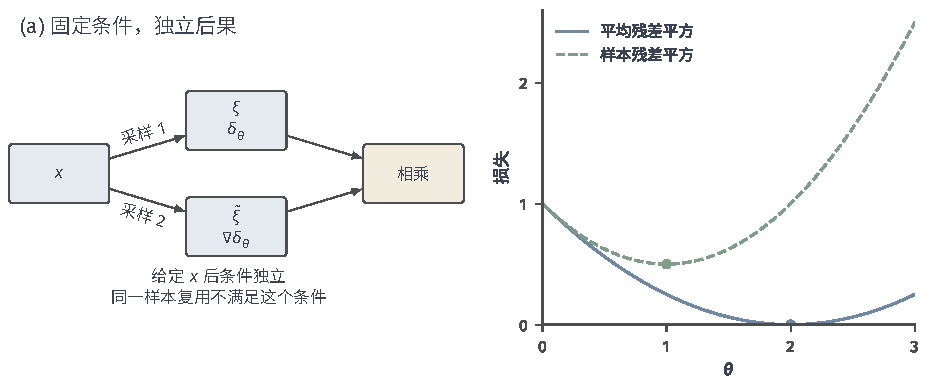
\includegraphics[width=157.406mm]{figures/10-reinforcement-learning/01-problems-and-solving/tikz/rl-learning-double-sampling.pdf}
  \caption{双重采样针对条件均值乘积。左侧两条独立支路保持同一个条件变量$x$；右侧曲线按示例\ref{ex:rl-learning-double-sampling}的解析公式绘制，展示两个损失的最小值不在同一参数处。}
  \label{fig:rl-learning-double-sampling}
\end{figure*}

常见的半梯度TD采取另一条路线：对自举目标停止求导，只执行
\[
  \bm{\theta}\leftarrow\bm{\theta}
       +\alpha\delta_{\bm{\theta}}
                    \nabla_{\bm{\theta}}V_{\bm{\theta}}(s).
\]
“半”表示没有求目标中下一价值对参数的导数。它不是式\eqref{eq:rl-learning-msbe-gradient}的随机梯度，因而不能借用该损失下降作为稳定性证明。在线性、同策略且采样权重与策略平稳分布匹配时，可用投影Bellman方程分析；离策略权重会破坏这条论证。表\ref{tab:rl-learning-fitted-methods}把这种逐步递推与批量方程、重复回归放在同一个评价或控制接口下比较。

在线性TD中，记$\bm\phi=\bm\phi(s)$、$\bm\phi'=\bm\phi(s')$，分别为当前和后继特征，撇号不是导数。平均更新为0要求$\mathbb E[\bm\phi\delta]=\bm0$；把$\delta=r+\gamma\bm\phi'^{\top}\bm\theta-\bm\phi^{\top}\bm\theta$代入并整理，就得到$\bm A\bm\theta=\bm b$。这里的期望按$s\sim d$、$a\sim\pi(\cdot\mid s)$、$(r,s')\sim p(\cdot,\cdot\mid s,a)$的固定策略样本计算；使用行为策略记录时需另作离策略校正。

这为批量求解提供了入口：最小二乘时序差分（least-squares temporal difference, LSTD）用许多记录估计$\bm A,\bm b$，再解方程；最小二乘策略迭代（least-squares policy iteration, LSPI）把这种动作值评价与贪心改进交替执行。拟合Q迭代（fitted Q-iteration, FQI）则不要求线性方程，而是每轮冻结旧$Q$，为记录构造新标签，再让回归器拟合。下面的表按这些不同求解任务汇总。

\begin{table*}[t]
  \centering
  \small
  \begin{tabularx}{\linewidth}{>{\raggedright\arraybackslash}p{23mm} >{\raggedright\arraybackslash}X >{\raggedright\arraybackslash}X}
    \toprule
    方法 & 解什么问题 & 表示、转移记录与适用边界 \\
    \midrule
    半梯度TD & 用样本逼近Bellman不动点，不对目标求全导数 & 线性同策略有专门保证；一般网络不是某个MSBE的下降法 \\
    LSTD & 解$\bm{A}\bm{\theta}=\bm{b}$，其中$\bm{A}=\mathbb E[\bm{\phi}(\bm{\phi}-\gamma\bm{\phi}')^\top]$、$\bm{b}=\mathbb E[r\bm{\phi}]$ & 固定策略线性评价；离策略版本需概率比等校正与矩阵可解条件 \\
    LSPI & 交替做动作值的LSTD评价与贪心改进 & 线性动作特征、同一批固定转移记录反复用于不同目标策略；需要相关状态动作覆盖 \\
    拟合Q迭代（FQI） & 冻结旧$Q$，回归$r+\gamma\max_aQ_{\mathrm{old}}(s',a)$ & 可用非线性回归器；控制误差包含回归误差、函数类封闭性与分布迁移 \\
    \bottomrule
  \end{tabularx}
  \caption{评价、控制与求解方式的差别。批量最小二乘减少逐步更新噪声，不会消除状态动作记录缺失或错误目标。}
  \label{tab:rl-learning-fitted-methods}
\end{table*}

\Needspace{20\baselineskip}
LSTD直接估计线性不动点方程的矩阵与向量，再求解参数\scite{rl3-bradtke1996lstd}
它省去逐步梯度迭代，但样本矩阵病态时仍需正则化和数值诊断，不能把可写成线性方程理解为总能稳定求逆。

LSPI把这种评价接口接到策略迭代：评价当前策略，按动作值改进，再重新构造与新策略相应的评价方程。固定转移样本的复用依赖行为策略记录对所需状态动作的覆盖，不是一次解线性方程便得到全局最优策略\scite{rl3-lagoudakis2003lspi}

FQI则冻结上一轮动作值，将新的Bellman目标交给监督回归器。它允许树模型等非梯度回归工具；每轮拟合误差以及从训练转移记录的状态动作抽样分布到部署策略访问分布的变化，仍会影响最终控制质量。三者提供了不同计算接口，不能只按是否使用梯度分类\scite{rl3-ernst2005tree}

一个完全线性的反例足以说明离策略、自举与共享参数同时出现的风险。Baird反例有7个状态、8个参数，奖励全为0，$\gamma=0.99$\scite{rl3-baird1995residual}
目标策略总选实线动作，转到状态7；行为策略以$1/7$选实线动作，以$6/7$选虚线动作，后者均匀转到上方6个状态。行为链的平稳分布为均匀分布。特征取
\[
  \bm{\phi}(i)=\frac{2\bm{e}_i+\bm{e}_8}{\sqrt5}\quad(1\leq i\leq6),
  \qquad
  \bm{\phi}(7)=\frac{\bm{e}_7+2\bm{e}_8}{\sqrt5}.
\]
令$\bm{\Phi}$的第$i$行为$\bm{\phi}(i)^\top$，$\bm{D}=\bm{I}/7$，$\bm{T}^\pi=\bm{1}\bm{e}_7^\top$。对带一步重要性比的半梯度TD，固定当前参数、按行为平稳样本取期望，漂移为
\begin{equation}
  \mathbb E[\Delta\bm{\theta}\mid\bm{\theta}]
     =\alpha\bm{M}\bm{\theta},\qquad
  \bm{M}=\bm{\Phi}^\top\bm{D}
                   (\gamma\bm{T}^\pi-\bm{I})\bm{\Phi}.
  \label{eq:rl-learning-baird-matrix}
\end{equation}
重要性比修正了给定状态的动作分布，却没有把行为状态权重$\bm{D}$换成目标状态权重。

在不变的对称子空间$\theta_1=\cdots=\theta_6=a$、$\theta_7=b$、$\theta_8=c$中，该漂移作用为
\begin{equation}
  \begin{pmatrix}\dot a\\\dot b\\\dot c\end{pmatrix}
  =
  \frac1{35}
  \begin{pmatrix}
    -4 & 1.98 & 1.96\\
     0 & -0.01 & -0.02\\
    -12 & 5.92 & 5.84
  \end{pmatrix}
  \begin{pmatrix}a\\b\\c\end{pmatrix}.
  \label{eq:rl-learning-baird-reduced}
\end{equation}
未除35的矩阵具有特征多项式$z(z^2-1.83z+0.26)$，因此漂移特征值为$0$、约$0.04785009$和$0.00443562$。例如较大的正特征值对应$(a,b,c)\approx(0.34124745,-0.01187117,1)$。若用期望更新作确定性迭代，沿这个方向每步乘$1+\alpha(0.04785009)>1$；在对应平均常微分方程中则指数增长。即使采用趋零且和发散的正步长，该方向的乘积仍不衰减。由此看到的是平均动力学的不稳定方向，而不只是某次随机运行的波动；随机更新还需相应随机逼近分析，不能把独立平稳样本的期望等式不加说明地当成任意相关轨迹下的参数均值递推。真实价值是0，函数类完全能表示它，问题出在更新动力学。

上述反例中，真实零价值在函数类内，平均更新仍有发散方向；单靠表示能力无法修复它。梯度TD方法为固定策略的线性评价改造目标和递推。对行为策略$\beta$的平稳经验，记$\bm\phi_t=\bm\phi(s_t)$、$\bm\phi_{t+1}=\bm\phi(s_{t+1})$，并用$\rho_t=\pi(a_t\mid s_t)/\beta(a_t\mid s_t)$校正动作分布；目标动作仍须由行为策略支持。由这些当前和后继特征定义不动点矩阵$\bm A$、奖励向量$\bm b$及特征二阶矩$\bm C$：
\[
  \bm{A}=\mathbb E_\beta[\rho_t\bm{\phi}_t
          (\bm{\phi}_t-\gamma\bm{\phi}_{t+1})^\top],\quad
  \bm{b}=\mathbb E_\beta[\rho_t r_t\bm{\phi}_t],\quad
  \bm{C}=\mathbb E_\beta[\bm{\phi}_t\bm{\phi}_t^\top].
\]
若$\bm C$正定，则MSPBE为
$(\bm b-\bm A\bm\theta)^\top\bm C^{-1}
 (\bm b-\bm A\bm\theta)$。

辅助向量的作用是把一个难直接估计的乘积拆开。令残差向量$\bm b-\bm A\bm\theta$固定，所需$\bm w$应满足$\bm C\bm w=\bm b-\bm A\bm\theta$；第一条递推用样本逐渐追踪这个解，第二条再用它调整价值参数。GTD2属于梯度时序差分（gradient temporal difference, GTD）方法，其2标识针对投影Bellman误差的版本。这里称双时间尺度，是要求$\bm w$的追踪比$\bm\theta$的变化快，近似形成“先估计当前需要的均值，再据它改变参数”的关系，而非必须开两种物理时钟。

GTD2用辅助向量$\bm w$跟踪$\bm C^{-1}(\bm b-\bm A\bm\theta)$，例如双时间尺度更新
\begin{align}
  \bm w&\leftarrow\bm w+\alpha_t^w
     [\rho_t\delta_t-\bm\phi_t^\top\bm w]\bm\phi_t,
     \nonumber\\
  \bm\theta&\leftarrow\bm\theta+\alpha_t\rho_t
     (\bm\phi_t-\gamma\bm\phi_{t+1})(\bm\phi_t^\top\bm w).
  \label{eq:rl-learning-gtd2}
\end{align}
辅助变量把难以直接估计的期望乘积拆成两个受控的递推，快变量在慢变量变化之前近似跟踪所需均值。

\Needspace{24\baselineskip}
GTD早期版本以期望TD更新的平方范数为目标；GTD2针对MSPBE；TDC采用TD加校正的形式，在同一线性目标下组织更新；emphatic TD则通过跟随迹重设状态权重，例如$F_t=i_t+\gamma\rho_{t-1}F_{t-1}$中$i_t$指定关注程度，以改变离策略投影的稳定性条件。它们并非都在优化同一个无权Bellman残差。收敛定理还需固定策略、特征与重要性比的矩条件、行为链覆盖、矩阵条件以及合适步长；双时间尺度分析常要求$\alpha_t/\alpha_t^w\to0$。这些评价结论没有直接证明深度控制稳定\scite{rl3-sutton2009fast,rl3-sutton2016emphatic}

% Outline: 3.2.6
\subsection{深度价值控制的训练机制}
\label{sec:rl-learning-dqn}

表格中更新一个状态动作，只修改一项数值。深度Q网络（deep Q-network, DQN）用神经网络一次输出或计算动作价值，同一参数会影响许多表项，还会进入后继目标。若每改一次预测，目标也立刻跟着改，训练就不断追逐正在移动的数值。先暂时固定一份旧参数来算标签，再让当前网络拟合它，承接了FQI的短期固定目标思路。

目标移动之外，连续采样还使相邻经验高度相关，少数极端TD误差也可能主导一次梯度。DQN用延迟参数生成目标，减缓自举目标随在线参数移动；把真实经验存入回放再抽样，减少相邻样本在训练批中的相关性；限制大误差的梯度幅度，避免极端残差主导更新。它们改变的是样本组织和短期回归过程，不是任意网络的收敛证明。

记有限回放记录组为$D$，按指定回放权重抽取记录的经验抽样律为$\widehat P_D$。其状态边缘记为$\widehat P_D^S$。每次训练按$\widehat P_D$取记录$(s,a,r,s',z)$，其中$z=1$仅表示环境真正终止。我们要减小在线网络对记录动作的预测与停止求导目标的差；目标先在$s'$的合法动作中找最高延迟估值，再加已观察奖励。记在线参数$\bm\theta$、延迟参数$\bar{\bm\theta}$，得到
\begin{equation}
  y=r+\gamma(1-z)\max_{a'\in\mathsf A(s')}Q_{\bar{\bm\theta}}(s',a'),
  \qquad
  L(\bm\theta)=\mathbb E_{\widehat P_D}
       \ell_\kappa\bigl(y-Q_{\bm\theta}(s,a)\bigr),
  \label{eq:rl-learning-dqn-loss}
\end{equation}
其中$\ell_\kappa(u)=u^2/2$当$|u|\leq\kappa$，否则为$\kappa(|u|-\kappa/2)$。这个Huber形式使大误差的导数限幅。$y$在该次更新中停止求导，目标网络不从这条损失直接反向传播。图\ref{fig:rl-learning-dqn}把两条参数路径分开。

\begin{figure*}[t]
  \centering
  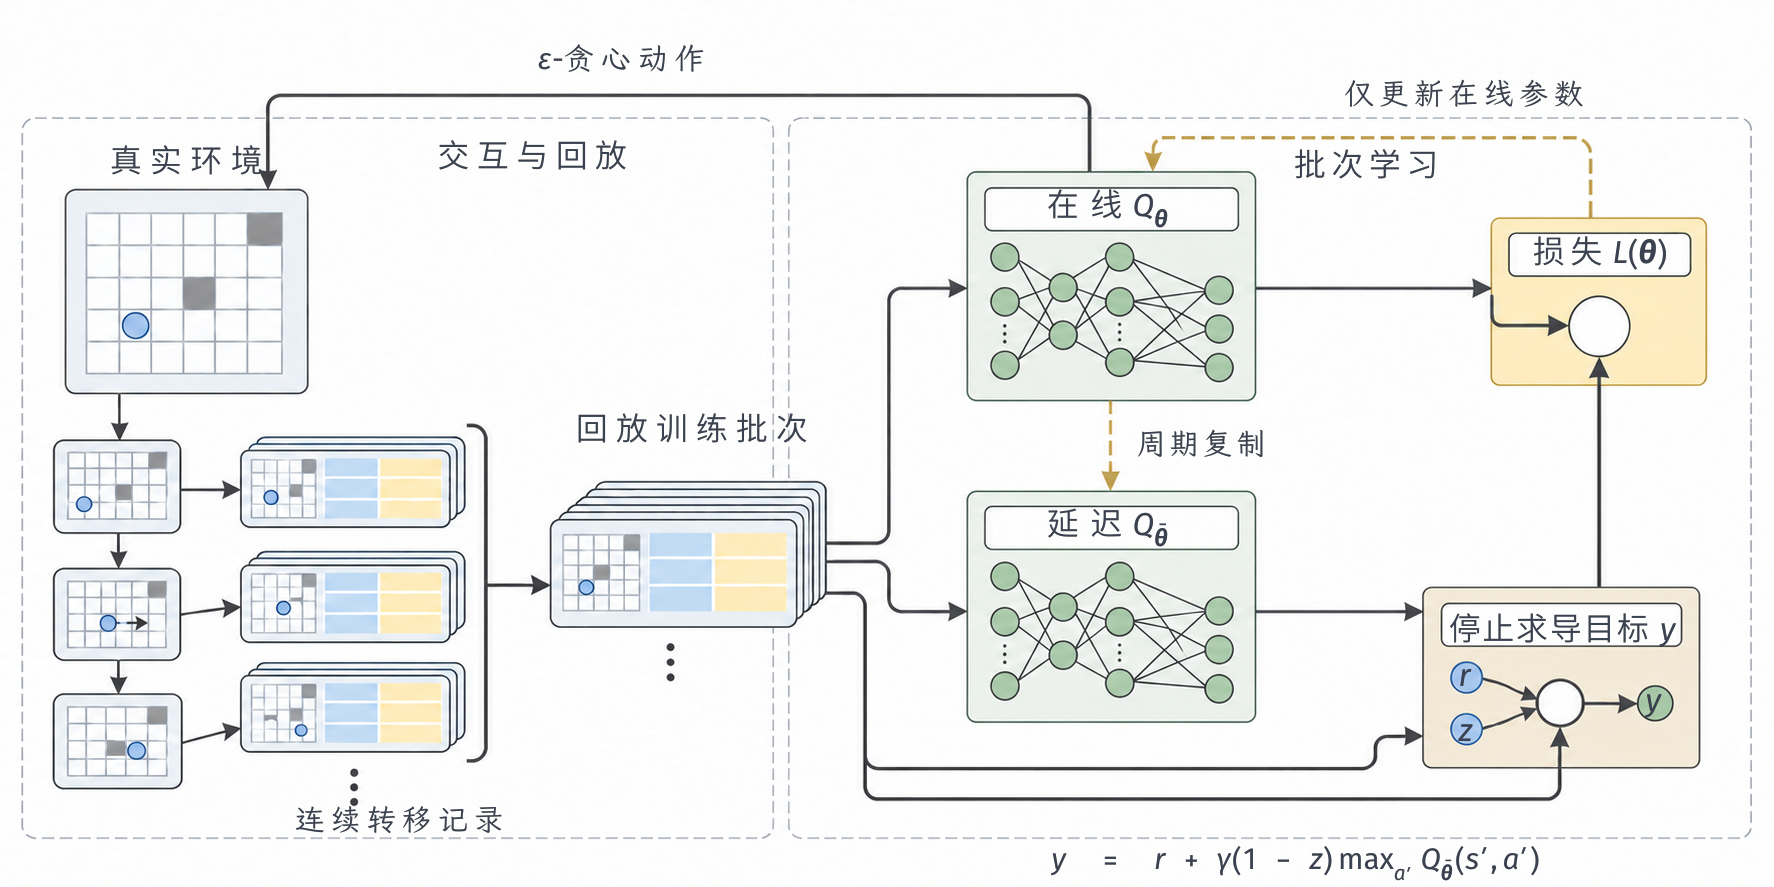
\includegraphics[width=157.400mm]{figures/10-reinforcement-learning/01-problems-and-solving/generated/rl-learning-dqn/figure.png}
  \caption{DQN的交互回放与批次学习。真实转移写入回放，在线网络给出被选动作的估值，延迟网络构造后继目标。在线与延迟网络之间的纵向虚线表示周期复制，外侧虚线表示只更新在线参数的损失梯度；目标分支停止求导。网格、记录卡片和神经节点仅示意部件职责，不规定基准网格布局、批量大小或网络结构。}
  \label{fig:rl-learning-dqn}
\end{figure*}

\begin{algorithm}[包含交互记录采集的DQN循环]
  \label{alg:rl-learning-dqn}
  \begin{algorithmic}[1]
    \Require 网络$\bm\theta$、空回放$D$、批量大小$B$、目标同步间隔$C$、更新频率、合法动作接口
    \State 置$\bar{\bm\theta}\gets\bm\theta$，从环境获得起始状态$s$
    \For{每个真实环境步$t$}
      \State 用当前$Q_{\bm\theta}$的$\varepsilon_t$-贪心策略在$\mathsf A(s)$中选择$a$
      \State 执行$a$，观察$r,s'$及真正终止标记$z$，将$(s,a,r,s',z)$写入$D$
      \If{已满足回放预热数量且到达更新时刻}
        \State 均匀抽取$B$条记录，按式\eqref{eq:rl-learning-dqn-loss}计算停止求导的目标$y_i$
        \State 对$B^{-1}\sum_i\ell_\kappa(y_i-Q_{\bm\theta}(s_i,a_i))$做规定次数梯度更新
      \EndIf
      \If{目标网络更新计数达到$C$}
        \State $\bar{\bm\theta}\gets\bm\theta$，重置同步计数
      \EndIf
      \State 若真正终止或环境因时间上限要求重置，则重置并取得新起点；否则令$s\gets s'$
      \State 仅时间截断的记录仍令$z=0$，并保留重置前的$s'$用于自举
    \EndFor
    \Ensure 在线网络及与训练探索策略区分的评估策略
  \end{algorithmic}
\end{algorithm}

算法\ref{alg:rl-learning-dqn}中的$C$按环境步还是梯度步计数必须在实现中固定。取示例\ref{ex:rl-learning-sarsa-q}的一条记录，若延迟网络最大值为$0.8$、在线被选动作值为$0.3$，则$y=0.68$、残差为$0.38$。当$\kappa=1$，对该输出的梯度为$-0.38$；在仅这一标量可训练、学习率$0.1$的教学网络中，新输出为$0.338$。真实共享网络还会改变其他状态动作，不能把这个标量更新当作一般网络输出的精确变化。

原始DQN在Atari像素输入、固定动作重复与预处理协议下检验了上述机制\scite{mnih2015}
回放减少相邻样本在同一批中的相关性，也允许同一真实经验参与多次更新；这不等于新增了独立采集的环境转移样本。目标网络固定一个短期回归目标，但同步时目标仍会改变。奖励裁剪也改变了训练目标，不能把所有具体设计视为任何任务都适用的定理。

后续部件针对不同的误差来源。表\ref{tab:rl-learning-dqn-components}保留每项实际改变的公式，便于区分表示改造、抽样改变与目标改变。优先回放中，$N$是当前缓冲区的记录数，$i$编号其中一条记录，$P(i)$是归一化抽样概率。指数$p\geq0$控制优先程度，$p=0$恢复均匀抽样；$\epsilon>0$使零残差记录仍有机会被抽到。校正指数$\eta_{\mathrm{IS}}\in[0,1]$控制向均匀缓冲目标补偿的程度，不是抽样概率本身。

有些状态中各动作的回报都差不多，逐动作独立表示会重复学习共同部分。Dueling结构把预测拆成状态共有的$V(s)$与动作差异$A(s,a)$，再对动作差异中心化；这里的$A$先表示网络输出之间的相对量。优先回放解决另一问题：同样抽一次记录，不同记录对当前误差的纠正作用可能不同，因而提高大残差记录的抽样概率，但这会改变经验损失的权重，需要相应校正。参数噪声则在一次扰动下共同改变许多动作评分，使探索发生在整份价值函数的参数上。这三个动机与Double DQN的选择偏差不同，下面分别列出机制。

NoisyNet式中的$\bm W,\bm M,\bm\Sigma,\bm E$形状相同；$\bm M$是可学习的均值权重，$\bm\Sigma$是可学习的噪声尺度系数，$\bm E$是每次扰动时抽取的零均值随机噪声，$\odot$表示逐元素乘法。训练调整前两者，噪声本身按所选分布重采样；这区分了学到的扰动强度和一次抽样结果。

\begin{table*}[t]
  \centering
  \small
  \begin{tabularx}{\linewidth}{>{\raggedright\arraybackslash}p{26mm} >{\raggedright\arraybackslash}X >{\raggedright\arraybackslash}X}
    \toprule
    部件 & 机制或公式 & 不能由它推出什么 \\
    \midrule
    Double DQN & 在线网络选$a^\star=\argmax_aQ_{\bm\theta}(s',a)$，延迟网络评价$Q_{\bar{\bm\theta}}(s',a^\star)$ & 两个网络仍相关，不能保证完全无偏 \\
    Dueling结构 & $Q(s,a)=V(s)+A(s,a)-|\mathsf A(s)|^{-1}\sum_bA(s,b)$ & 分解改善共享表示，不代表学到了独立可识别的真实优势 \\
    优先回放 & $P(i)\propto(|\delta_i|+\epsilon)^p$，权重$w_i\propto(NP(i))^{-\eta_{\mathrm{IS}}}$ & 非均匀抽样改变损失权重；$\eta_{\mathrm{IS}}<1$通常只作部分校正 \\
    NoisyNet & 权重写成$\bm W=\bm M+\bm\Sigma\odot\bm E$，学习噪声尺度 & 参数噪声与逐步随机动作不同，不自动保证长程覆盖 \\
    \bottomrule
  \end{tabularx}
  \caption{深度价值学习中的四种机制。它们分别改变目标、表示、回放记录抽样和探索参数，不能只用“更稳定”概括。}
  \label{tab:rl-learning-dqn-components}
\end{table*}

Double DQN在目标中分开动作选择与评价，避免同一次最大化总是同时选中偏高噪声。在线网络与目标网络仍共享训练历史，因此这不是两个独立无偏估计器，改动也不自动消除所有过估计\scite{rl3-hasselt2016deep}

Dueling用均值中心化消除$V$与$A$任意加减常数的代数歧义，使不同动作能够共享状态评价。但中心化后的$A$不必等于某个给定策略的真实优势；它首先是网络分解中的一个参数化量\scite{rl3-wang2016dueling}

优先回放若以固定缓冲区的均匀经验损失为目标，取$\eta_{\mathrm{IS}}=1$并保留正确的$1/(NP(i))$因子，可以对当前抽样分布校正；常见的批内最大值归一化、过期优先级和逐渐增加$\eta_{\mathrm{IS}}$都需要单独说明\scite{rl3-schaul2016prioritized}

\Needspace{28\baselineskip}
NoisyNet把可学习噪声加入网络参数，一次参数扰动会同时影响多个动作评分，其作用范围不同于逐步$\varepsilon$随机动作\scite{rl3-fortunato2018noisy}
噪声采样频率和尺度学习规则决定探索的时间相关性，但参数随机并不自动保证访问到远处关键状态。

组合系统必须用受控消融解释。Rainbow在57个ALE游戏、2亿帧训练的具体配置中，逐一去掉Double、优先回放、dueling、多步、分布式目标和参数噪声等组件；论文中的优先回放与多步移除影响较大，Double与dueling对中位汇总的影响较小且依游戏而异。这是已组合系统内的条件贡献，不是组件在所有任务上的独立效应。其评估每隔一百万环境步进行一次，并使用最好快照，还涉及no-op和human-starts协议；因此不能把报告值当作预先约定最终检查点的无选择偏差估计\scite{rl3-hessel2018rainbow}

Agent57进一步结合内外在价值、跨时间尺度策略族、回合级元控制器及更长的序列训练。它回答的是更强探索与记忆如何组成系统，不是与Rainbow使用相同总预算的一次单因素试验。把论文中的表现差异归因于某一个部件，必须先统一交互、网络、回放与评估口径；无法统一时，只陈述各自协议下的证据。需要过去观测与动作记录的DRQN与R2D2将在第\ref{chap:rl-information}章讨论，不能把缺少过去观测与动作记录简单归为网络太小\scite{rl3-badia2020agent57}

% Outline: 3.2.7
\subsection{回报分布与控制充分表示}
\label{sec:rl-learning-distributional}

两个动作的期望回报相同，实际后果仍可能很不同。在独立教学例中，路径A总回报恒为$0.5$，路径B等概率得到$-0.5$或$1.5$；均值均为$0.5$，但只有B会出现较低和较高的结果。只存一个均值无法保留这项区别。这里另设了奖励分布，并不声称基准网格存在这两条精确路径；图\ref{fig:rl-learning-return-distributions}展示的就是这两个指定分布。

令$Z^\pi(s,a)$为给定状态动作之后的随机折扣回报。\term{分布式价值学习}（distributional value learning）学习的是整个回报分布，而非仅其均值。分布Bellman关系为
\begin{equation}
  Z^\pi(s,a)\ \overset{D}{=}\ %
    r+\gamma Z^\pi(s',a'),\qquad
  (s',r)\sim p(\cdot,\cdot\mid s,a),\quad a'\sim\pi(\cdot\mid s').
  \label{eq:rl-learning-distributional-bellman}
\end{equation}
右侧的未来随机回报按给定$s',a'$的条件分布抽取，不能误把它理解成一条确定性递推。

\begin{figure}[htbp]
  \centering
  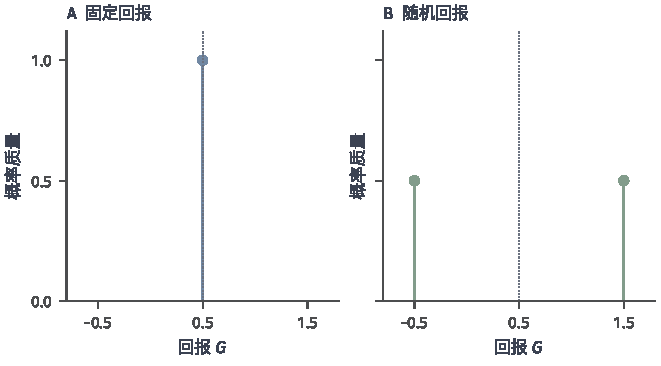
\includegraphics[width=112.000mm]{figures/10-reinforcement-learning/01-problems-and-solving/matplotlib/rl-learning-return-distributions.pdf}
  \caption{相同期望不意味着相同回报分布。两图为人工指定的离散分布，虚线均位于期望$0.5$；这里的不确定性是回报本身的随机性，不是估计参数的置信区间。}
  \label{fig:rl-learning-return-distributions}
\end{figure}

表示一个分布，需要决定保存哪些回报值和多少概率。可以预先固定回报刻度，让模型学习每一刻度附近有多少质量；也可以固定概率刻度，让模型学习对应的回报位置。后一种位置是分位数：$\tau$分位把回报划分到至少$\tau$的概率不超过该值、至少$1-\tau$的概率不低于该值。离散分布可能没有唯一分位位置，后文会给出精确的不等式条件。分位输出与均值输出回答不同问题，不能用普通对称平方误差训练后就称其为分位数。

C51把质量放在固定支撑点$z_1,\ldots,z_N$上，学习各点概率；Bellman变换后的原子$r+\gamma z_j$要按距离插值投影回固定支撑，支撑范围之外的质量会被截到端点。QR-DQN反过来固定每个原子的概率$1/N$，学习分位位置$\theta_i(s,a)$；IQN以随机分位水平$\tau$作为网络输入，表示一个条件分位函数。这三个表示对支撑范围、分辨率和采样方式的限制不同。

要学习分位位置，需要让高分位输出对正残差比负残差更敏感，而不是像平方回归那样都追向均值。以分位回归为例，令$\tau_i=(i-\tfrac12)/N$，$a^\star$是在后继合法动作中按估计均值选出的贪心动作，目标样本为$z'_j=r+\gamma\theta_j(s',a^\star)$。对$u=z'_j-\theta_i(s,a)$，将Huber误差按分位水平非对称加权，再对全部$N^2$对输出和目标平均：
\[
  \rho_{\tau_i}^{\kappa}(u)
      =|\tau_i-\mathbf1\{u<0\}|\frac{\ell_\kappa(u)}{\kappa},
  \qquad
  L=\frac1{N^2}\sum_{i,j}\rho_{\tau_i}^{\kappa}(z'_j-\theta_i).
\]
正负残差的不对称权重使训练朝所需分位方向调整，而Huber阈值$\kappa>0$平滑了零残差附近的目标。例如$\tau_i=0.75$、$u=0.4$、$\kappa=1$时损失为$0.75(0.4^2/2)=0.06$；同样大小的负残差只乘$0.25$。这说明非对称性，不保证有限$\kappa$下的总体最小点正好等于指定分位。

作为对照，标准非平滑分位损失为$\rho_\tau(u)=|\tau-\mathbf1\{u<0\}|\,|u|$。对$\tau\in(0,1)$和一阶可积目标$Y$，最小化$\mathbb E\rho_\tau(Y-\theta)$的解满足$\mathbb P(Y<\theta)\leq\tau\leq\mathbb P(Y\leq\theta)$，即为该水平的分位解；分位不唯一时也不保证单一输出位置。有限阈值的Huber形式是平滑训练代理，会改变这个精确性质。例如$Y$等概率取0和1、$\tau=0.75$、$\kappa=1$时，对$\theta\in[0,1]$的总体代理为$\theta^2/16+3(1-\theta)^2/16$，最小点为$0.75$，而该分布的$0.75$分位为1。因而学到的平滑输出不能无条件解释成准确分位；去掉非对称权重则连分位方向也不再保留\scite{rl3-bellemare2017distributional,rl3-dabney2018quantile,rl3-dabney2018implicit}

比较两个回报分布时，要计量的不只是概率差，还包括回报数值相隔多远。对实值回报分布$\mu,\nu$及$1\leq p<\infty$，$p$-Wasserstein距离为
\[
  W_p(\mu,\nu)=
    \inf_{\lambda\in\Gamma(\mu,\nu)}
       \left(\mathbb E_{(X,Y)\sim\lambda}|X-Y|^p\right)^{1/p}.
\]
这里$\Gamma(\mu,\nu)$包含所有第一边缘为$\mu$、第二边缘为$\nu$的联合分布，称为两分布的耦合。它允许比较不同的配对方式，但不得改变任一边的回报分布；下确界选择平均$p$次差最小的配对，再开$p$次根恢复回报尺度。对两族状态动作回报分布$\mathcal Z,\widetilde{\mathcal Z}$，采用
$\bar W_p=\sup_{s\in S,\,a\in\mathsf A(s)}
W_p(\mathcal Z(s,a),\widetilde{\mathcal Z}(s,a))$，
有限状态动作时就是最大值。这要求统一控制每个合法状态动作，不能只让常见位置的平均距离小。

在固定策略且上述$p$阶矩统一有界的条件下，分布Bellman算子在$\bar W_p$下是$\gamma$压缩。两边可共用同一次奖励、后继状态和按固定策略选出的后继动作，再耦合各自的未来回报；奖励相消，未来数值差乘$\gamma$，对条件分布平均后仍受$\gamma\bar W_p$控制。控制时依据均值取最大动作，动作切换会破坏直接沿用这一论证的条件。即使完整学到$Z^\pi$，若仍按期望最大化，也没有自动引入风险厌恶；风险目标将在第\ref{chap:rl-trustworthy}章另定。回报分布同样不能自动表示“这条分布是用多少样本估出来的”。

分布Bellman式中的$\overset D=$表示两边有同一概率分布，并不要求两次独立抽到的回报数值相等。固定策略时，两套预测可以共用同一个随机奖励和后继，只比较各自尚余的未来回报；折扣才会把这部分数值差缩小。这里控制的是回报分布之间的差别，不是对训练参数有多少把握，所以它仍不能代替探索所需的置信区间。

回报表示保留了一个状态动作的结果分布，状态表示则决定哪些不同状态可共用预测。合并状态时，至少要避免把奖励或未来决策机会不同的状态当成同一个。设映射$f:S\to\bar{S}$；具有同一像的状态构成一个等价类。若任意同类状态$s_1,s_2$都有完整相同的合法动作域$\mathsf A(s_1)=\mathsf A(s_2)$，并对这个共同域中的每个动作具有相同奖励均值，且进入每个等价类$C$的概率也相同，即
\[
  \sum_{s'\in C}T(s'\mid s_1,a)
       =\sum_{s'\in C}T(s'\mid s_2,a),
\]
那么控制Bellman备份可以在等价类上闭合：类内相同动作产生相同的一步奖励和后继类价值，最大化的候选域也相同，所以备份结果不依赖选哪个类成员。只检查两状态共有动作不够，某个状态独有的高奖励动作就可能改变最大值。这是双模拟的重要条件；MDP同态还可以包含状态相关的动作映射，但映射须保留可用动作及对应的奖励和类转移。价值等价则只要求对指定策略与价值测试函数保留相关备份，不一定保留全部观测或完整转移分布，必须说明测试类有多大。

另设一个只提供局部图像的导航例：两个视觉几乎相同的走廊端点，一个只能向上绕过障碍，另一个向下才接近终点。若编码器只看局部纹理并把它们合并，同一个潜在状态就无法同时给出正确动作。这个反例改变了基准网格的地图与观测接口；它说明局部图像未必能替代马尔可夫状态。相反，两个外观不同但合法动作域、各动作奖励和后继等价类概率都相同的状态可以在控制上等价。像素重建相似与控制充分性不是同一判据\scite{rl3-givan2003equivalence}

价值等价进一步围绕所需策略与价值测试函数定义模型要保留的内容。缩小测试集合可以降低学习要求，却也缩小了结论范围；不能在一个策略集合上检验等价后，直接推广到任意后续搜索和任务\scite{rl3-grimm2020value}

表\ref{tab:rl-learning-representations}沿监督信号比较几种表示方法。要从辅助目标走到控制结论，还应检查它是否保留了动作后果，而不只看特征是否易于预测。

\begin{table*}[t]
  \centering
  \small
  \begin{tabularx}{\linewidth}{>{\raggedright\arraybackslash}p{22mm} >{\raggedright\arraybackslash}X >{\raggedright\arraybackslash}X}
    \toprule
    表示方法 & 监督信号 & 希望保留的性质及边界 \\
    \midrule
    DeepMDP & 潜在转移与奖励预测损失 & 在相应误差、距离和光滑条件下连接价值；有限训练损失不等于满足全局条件 \\
    CURL & 同一观测不同增强的对比目标 & 提高表示一致性；正样本增强必须不抹掉会改变动作后果的观测差别 \\
    SPR & 动作条件多步潜在预测与目标表示匹配 & 保留时间与动作相关结构；预测存在不代表执行时查询模型规划 \\
    DrQ & 对增强观测计算并正则化价值学习目标 & 用合理增强约束价值一致性；不是环境转移模型 \\
    \bottomrule
  \end{tabularx}
  \caption{辅助表示目标与控制接口。理想结构保证、训练损失和实际测试表现应分别陈述。}
  \label{tab:rl-learning-representations}
\end{table*}

\Needspace{20\baselineskip}
DeepMDP把奖励与潜在转移预测联系到价值误差；相关条件针对指定距离、误差和光滑性，不是仅凭训练集重建分数判断表示充分\scite{rl3-gelada2019deepmdp}

CURL用同一观测的不同增强构造正样本，使表示在这些变化下保持一致。增强若抹去了会改变动作后果的观测差别，对比目标做得好反而可能使控制更难，因此增强设计也是任务假设\scite{rl3-laskin2020curl}

\Needspace{20\baselineskip}
SPR用动作条件的多步预测约束表示，使潜在特征保留部分时间关系。辅助预测不意味着执行时一定查询它作规划；分类仍应看策略改进实际读取的观测、表示及预测目标\scite{rl3-schwarzer2021spr}

DrQ把图像增强接到价值目标与评价中，通过同一训练观测的不同增强视图约束价值估计。它改变的是训练图像观测的处理与正则化方式，不要求学习一个可滚动的环境转移模型\scite{rl3-kostrikov2021drq}

% Outline: 3.2.8
\subsection{价值误差与策略性能}
\label{sec:rl-learning-value-performance}

估值是否有用，最终取决于它选出的动作能取得多少回报。下面先假定每个合法状态动作的估计都与$Q^*$相差至多$\epsilon$，据此控制贪心策略的损失；这里的无穷范数取遍全部合法状态动作，而非只平均训练样本。这个较强条件避免了关键岔路被平均权重掩盖，也让选错动作的代价可以逐步累加。

\begin{theorem}[动作价值误差到贪心策略损失]
  \label{thm:rl-learning-q-performance}
  设$S$有限，各非终止状态的合法动作集有限且非空，奖励有界，$0\leq\gamma<1$。对$\epsilon\geq0$，若动作价值函数$q$满足$\lVert q-Q^*\rVert_\infty\leq\epsilon$，且$\pi_q$在每个状态按固定并列规则选择$q$的最大合法动作，则
  \begin{equation}
    \lVert V^*-V^{\pi_q}\rVert_\infty
       \leq\frac{2\epsilon}{1-\gamma}.
    \label{eq:rl-learning-q-performance}
  \end{equation}
\end{theorem}
\begin{proof}
  固定$s$，令$a^*\in\argmax_aQ^*(s,a)$、$a_q=\pi_q(s)$。由贪心性$q(s,a_q)\geq q(s,a^*)$，
  \[
    Q^*(s,a^*)-Q^*(s,a_q)
      \leq[Q^*(s,a^*)-q(s,a^*)]
            +[q(s,a_q)-Q^*(s,a_q)]\leq2\epsilon.
  \]
  又因$Q^*(s,a_q)=R(s,a_q)+\gamma\mathbb E[V^*(s')\mid s,a_q]$，
  \[
    V^*(s)-V^{\pi_q}(s)
      \leq2\epsilon+\gamma
          \mathbb E[V^*(s')-V^{\pi_q}(s')\mid s,a_q].
  \]
  沿$\pi_q$展开$n$步，右边为
  $2\epsilon\sum_{t=0}^{n-1}\gamma^t$
  加上$\gamma^n\mathbb E[V^*(s_n)-V^{\pi_q}(s_n)]$。有限折扣任务价值有界，尾项随$n\to\infty$消失，得到逐状态上界，再取无穷范数。
\end{proof}

两次误差分别对应高估被选动作和低估真正最优动作，$1/(1-\gamma)$则来自沿途重复作出次优选择。这也解释了为什么不能把“某批训练样本上的均方误差很低”直接代入定理。表\ref{tab:rl-learning-value-bounds}将这一结论与状态值前瞻及当前策略评价并列，关键区别在误差究竟相对谁定义。

\begin{table*}[t]
  \centering
  \small
  \begin{tabularx}{\linewidth}{>{\raggedright\arraybackslash}p{31mm} >{\raggedright\arraybackslash}X >{\raggedright\arraybackslash}X}
    \toprule
    已知误差 & 如何选动作 & 相应结论或限制 \\
    \midrule
    $\lVert q-Q^*\rVert_\infty\leq\epsilon$ & 直接最大化$q(s,a)$ & 最优性能损失至多$2\epsilon/(1-\gamma)$ \\
    $\lVert v-V^*\rVert_\infty\leq\epsilon$ & 用准确模型最大化$R+\gamma Tv$ & 与规划章相同的$2\gamma\epsilon/(1-\gamma)$界；多一个$\gamma$来自一次前瞻 \\
    $\lVert q-Q^\pi\rVert_\infty\leq\epsilon$ & 对当前策略的近似评价作贪心改进 & 支持相对$\pi$的近似改进分析，不是相对$Q^*$的同一界 \\
    训练分布均方误差较小 & 取决于部署访问状态 & 还需覆盖、分布比或其他误差转移条件 \\
    \bottomrule
  \end{tabularx}
  \caption{动作值和状态值的用途差异。状态值本身不能在未知模型中完成一步动作比较。}
  \label{tab:rl-learning-value-bounds}
\end{table*}

考虑从网格岔路抽出的独立终止决策例：到岔路必选左或右，真实回报分别为1和0；训练状态动作抽样分布却只有$10^{-3}$质量落在这两个动作上，其余状态估计完全准确。若$q$在岔路把两值颠倒，则训练均方误差仅为$10^{-3}$，部署损失却为1。图\ref{fig:rl-learning-error-flow}左侧显示错误集中位置，右侧串起误差来源。训练样本中“少见”不能替代任务中“不重要”。

\begin{figure*}[t]
  \centering
  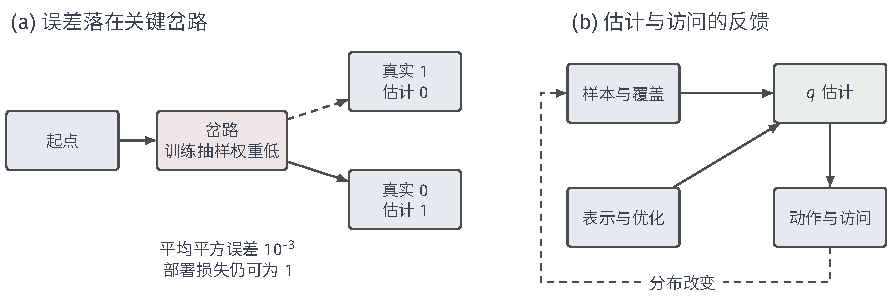
\includegraphics[width=150.887mm]{figures/10-reinforcement-learning/01-problems-and-solving/tikz/rl-learning-error-flow.pdf}
  \caption{局部错误与整体行为。左侧为人工指定的岔路反例，右侧区分表示、样本、优化及分布转移误差；图中的箭头是因果接口，不声称这些误差可以不加条件地线性相加。}
  \label{fig:rl-learning-error-flow}
\end{figure*}

表示误差决定函数类能否同时容纳关键区别，样本误差决定有限观测能否辨清回报，优化误差决定训练是否找到所要求的解；部署策略又可能访问训练中罕见的区域。这些环节必须分别检查。下一节改变主要优化对象，直接更新策略参数，但评论家误差与训练记录的覆盖不足并不会因此消失。

% Outline: 3.3
\section{无模型的策略优化}
\label{sec:rl-learning-policy}

连续控制力有无穷多取值，难以像表格动作那样逐个比较；即使只有上下左右，贪心动作也可能在估值稍有变化时突然切换。若希望直接调整控制输出或平滑改变动作概率，就可以参数化从状态到动作的映射，并按回报更新其参数。这称为\term{策略优化}（policy optimization）。无模型策略优化的更新不查询学得的动力学模型；价值估计器可以指导改变方向，却不负责预测环境转移。

这条路线的训练变量是策略参数，不要求先得到最优$Q$再作贪心选择。为估计更新方向，仍可配一个价值预测器：它为策略比较本次行动与通常回报，称为评论家；产生动作的策略称为行动者。先从不用评论家、只用采样回报的更新开始，随后再引入价值基线和两者的联合训练，这样可以分清价值预测承担的是辅助评价还是最终动作选择。

% Outline: 3.3.1
\subsection{策略梯度与回报梯度估计}
\label{sec:rl-learning-policy-gradient}

先考虑怎样从随机轨迹求出策略参数的上升方向。我们暂用有限状态动作和固定时域$H$，以便逐项对轨迹概率求导；策略$\pi_{\bm\theta,t}(a\mid s)$可依赖时间，在所讨论参数邻域内可微，并对合法动作严格为正。初始分布和环境核不依赖$\bm\theta$，奖励有界。记轨迹$\tau=(s_0,a_0,r_0,\ldots,s_H)$，用其折扣奖励和的期望比较候选参数，目标是增大$J_H$；$G_t^H$则保存动作$t$以后仍可影响的回报：
\begin{equation}
  J_H(\bm\theta)=\mathbb E_{\tau\sim P_{\mathcal E}^{\pi_{\bm\theta}}}
      \left[\sum_{t=0}^{H-1}\gamma^t r_t\right],
  \qquad
  G_t^{H}=\sum_{k=t}^{H-1}\gamma^{k-t}r_k .
  \label{eq:rl-learning-finite-policy-objective}
\end{equation}
策略的随机性提供了一个可求导的概率模型。无需知道某次动作怎样改变后继状态的导数，也能利用“这次轨迹的概率如何随参数变化”来估计回报梯度。

先把这种求导缩到一个单步两动作任务。设动作1奖励恒为$0.7$，动作2奖励恒为$0.4$，策略以$p=\sigma(\theta)=1/(1+e^{-\theta})$选择动作1。其期望回报为$J(\theta)=0.7p+0.4(1-p)$，直接求导得到$J'(\theta)=0.3p(1-p)$。如果不知道两个奖励，只能抽一个动作，仍可计算已选动作的对数概率导数：选动作1时为$1-p$，选动作2时为$-p$。把它乘实际奖励，平均得到
\[
 p\,0.7(1-p)+(1-p)\,0.4(-p)=0.3p(1-p).
\]
这个平均恰等于所需梯度，而一次样本只用到了策略概率和已观察奖励。对数概率的梯度称为得分函数（score function）；它说明当前参数变化会提高还是降低这次动作的发生概率。两种动作的样本方向可能相反，只有在抽样平均后才得到期望回报的上升方向。

推广到轨迹时，动作概率相乘，对数概率就相加；再用$\nabla p=p\nabla\log p$，可以把概率的导数写成“按原概率抽样后，对数梯度乘回报”的期望。这称为似然比估计，不需要对未知转移规律求导。下面的定理还会去掉每个动作之前已发生的奖励，因为这些奖励不能再受该动作影响。

\begin{theorem}[有限时域似然比策略梯度]
  \label{thm:rl-learning-likelihood-gradient}
  设状态空间$S$有限，每个非终止状态的合法动作集$\mathsf A(s)$有限且非空，$H\geq1$为整数，$0\leq\gamma\leq1$。初始分布及联合奖励转移核不依赖参数$\bm\theta$，奖励有界。在一个开参数邻域内，各$\pi_{\bm\theta,t}(\cdot\mid s)$均为合法动作上的严格正概率分布，且关于$\bm\theta$连续可微。用式\eqref{eq:rl-learning-finite-policy-objective}定义$J_H$和$G_t^H$。令
  $\bm z_t=\nabla_{\bm\theta}\log\pi_{\bm\theta,t}(a_t\mid s_t)$，则
  \begin{equation}
    \nabla_{\bm\theta}J_H
       =\mathbb E\left[
          \sum_{t=0}^{H-1}\gamma^t\bm{z}_tG_t^H\right].
    \label{eq:rl-learning-reward-to-go}
  \end{equation}
\end{theorem}
\begin{proof}
  轨迹分布分解为
  \[
    P_{\mathcal E}^{\pi_{\bm\theta}}(\mathrm d\tau)=\mu_0(s_0)
       \prod_{t=0}^{H-1}
       \pi_{\bm\theta,t}(a_t\mid s_t)
       p(\mathrm dr_t,s_{t+1}\mid s_t,a_t).
  \]
  环境项的导数为0，因此
  $\nabla P_{\mathcal E}^{\pi_{\bm\theta}}(\mathrm d\tau)
  =P_{\mathcal E}^{\pi_{\bm\theta}}(\mathrm d\tau)\sum_t\bm{z}_t$。
  该恒等式按测度理解，不要求奖励有离散点概率。有限状态动作和有限时域下，可以对策略概率的有限和逐项求导；随机奖励的有界性保证相应积分可交换。于是
  \[
    \nabla J_H
      =\mathbb E\left[
        \sum_{t=0}^{H-1}\bm{z}_t
        \sum_{k=0}^{H-1}\gamma^k r_k\right].
  \]
  令$I_t$为抽取$a_t$前的全部历史，则
  \[
    \mathbb E[\bm{z}_t\mid I_t]
       =\sum_a\pi_{\bm\theta,t}(a\mid s_t)
          \nabla\log\pi_{\bm\theta,t}(a\mid s_t)
       =\nabla\sum_a\pi_{\bm\theta,t}(a\mid s_t)=\bm0.
  \]
  当$k<t$时，$r_k$已经包含在$I_t$中，故
  $\mathbb E[\bm{z}_t r_k]=\bm0$。删去这些过去奖励，余下
  $\sum_{k=t}^{H-1}\gamma^k r_k=\gamma^tG_t^H$，即得结论。
\end{proof}

过去奖励的删除依据是得分函数对抽样前历史的条件均值为0；未来奖励前的时间权重并未消失。每个动作仍按$\gamma^t$计入起点目标。以$N$条独立同策略回合的
$N^{-1}\sum_{i,t}\gamma^t\bm{z}_{i,t}G_{i,t}^H$
作更新方向，就是一种REINFORCE估计。完整回报包含环境噪声与之后所有动作的随机性，因而无偏不等于低方差；但它不要求对环境转移求导\scite{rl1-williams1992-reinforce}

有限时域公式按时刻累加贡献。推广到无限折扣任务时，可以把这些访问概率汇总成一个状态分布，但需要先保证无限求和与求导可交换。采用平稳策略，并要求例如奖励与邻域内得分函数$\nabla\log\pi_{\bm\theta}$一致有界，就能对折扣级数及导数建立可积支配。再将给定状态动作的平均未来回报写成$Q^{\pi_{\bm\theta}}$，得到
\begin{equation}
  \nabla_{\bm\theta}J(\bm\theta)
    =\frac{1}{1-\gamma}
      \mathbb E_{\substack{s\sim d^{\pi_{\bm\theta}}\\
                           a\sim\pi_{\bm\theta}(\cdot\mid s)}}
        \left[\nabla_{\bm\theta}\log\pi_{\bm\theta}(a\mid s)
              Q^{\pi_{\bm\theta}}(s,a)\right].
  \label{eq:rl-learning-policy-gradient}
\end{equation}
这里$d^\pi$始终是归一化折扣占用分布，$J$始终是未归一化回报。若从固定长度回合中均匀抽时间步，却省去$\gamma^t$，所得权重通常不是$d^\pi$；调节学习率可以吸收整体常数，却不能修正不同时间步的相对权重。平均奖励目标、几何随机终止采样或特定工程近似各有自己的口径，不应把它们都称为式\eqref{eq:rl-learning-policy-gradient}的精确实现\scite{rl3-sutton2000policy}

归一化折扣占用可理解为一份带时间权重的访问记录：$d^\pi(s)=(1-\gamma)\sum_{t\geq0}\gamma^t\mathbb P_\pi(s_t=s)$。所有状态权重相加为1，所以它是概率分布；较早访问权重较大，较晚访问逐步折扣。策略梯度原来按时刻累加，改为从这份分布平均时，就要乘回$1/(1-\gamma)$。这个常数恢复总权重，不能将均匀时间抽样中各时刻相对权重的错误也一并修正。

表\ref{tab:rl-learning-policy-search-information}比较了三种改变策略的路径。确定性策略梯度将在后文展开；此处重要的是，参数可调并不意味着必须使用似然比，也不意味着能够穿过环境反向传播。

\begin{table*}[t]
  \centering
  \small
  \begin{tabularx}{\linewidth}{>{\raggedright\arraybackslash}p{29mm} >{\raggedright\arraybackslash}X >{\raggedright\arraybackslash}X}
    \toprule
    更新路径 & 所需奖励、概率或导数 & 不要求什么，以及主要代价 \\
    \midrule
    REINFORCE & 策略概率或密度及其对数梯度，采样回报 & 不求环境导数；长回合的梯度方差可能很大 \\
    确定性策略梯度 & 策略对参数的导数，$Q(s,a)$对动作的导数 & 不枚举连续动作；依赖评论家的动作方向导数 \\
    参数黑盒搜索 & 给定一组策略参数后可评估回报 & 不要求策略或环境可微；需支付多组参数的整轨迹评估成本 \\
    \bottomrule
  \end{tabularx}
  \caption{直接优化策略时的三类奖励、概率与导数需求。表中“无需模型导数”不等于“无需真实交互”。}
  \label{tab:rl-learning-policy-search-information}
\end{table*}

% Outline: 3.3.2
\subsection{基线、优势与方差控制}
\label{sec:rl-learning-baseline}

在本来就容易获得高回报的状态，许多动作都可能得到较大的$G_t$。直接以$G_t$加权，某次抽中的动作会因此获得很大更新，即使它没有优于其他动作；这些偶然更新可以在平均后相消，却增加了有限样本波动。\term{基线}（baseline）为回报设一个比较水平。若这个水平在本轮选动作之前已确定，减去它不会改变平均梯度，并可能去掉与本轮动作优劣无关的波动。

\begin{theorem}[动作抽样前基线的零均值性质]
  \label{thm:rl-learning-baseline}
  设$I_t$为抽取动作前的决策历史，其当前状态为$s_t$。在有限非空合法动作集$\mathsf A(s_t)$上，$a_t$按严格正、关于$\bm\theta$连续可微的概率分布$\pi_{\bm\theta,t}(\cdot\mid s_t)$抽取。设实基线$b_t$对$I_t$可测，且$b_t\nabla_{\bm\theta}\log\pi_{\bm\theta,t}(a_t\mid s_t)$可积。则
  \[
    \mathbb E[\nabla_{\bm\theta}
       \log\pi_{\bm\theta,t}(a_t\mid s_t)b_t]=\bm0.
  \]
  因而在式\eqref{eq:rl-learning-reward-to-go}中以$G_t^H-b_t$替换$G_t^H$，不改变期望梯度。
\end{theorem}
\begin{proof}
  条件于$I_t$，基线是常数，故
  \[
    \mathbb E[\bm{z}_t b_t\mid I_t]
      =b_t\sum_a\pi_{\bm\theta,t}(a\mid s_t)
                    \nabla\log\pi_{\bm\theta,t}(a\mid s_t)
      =b_t\nabla 1=\bm0.
  \]
  再对历史取期望，逐时刻相加即可。基线是否准确没有进入等式；进入等式的是它对本轮动作抽样的条件独立性。
\end{proof}

在单步两动作算例中，$p=1/2$时平均回报为$0.55$。取基线$0.55$，两个动作的超额回报为$0.15$和$-0.15$，对数梯度分别为$0.5$和$-0.5$，两种样本的乘积都为$0.075$。原来两个方向相反的样本，这时给出同一方向；平均梯度仍为$0.3(1/2)(1/2)=0.075$。这个确定性奖励例展示了基线如何去掉共同回报水平，不表示任意基线都能消除随机环境中的波动。

若以真实$V^\pi(s)$为基线，再按动作后的未来取平均，就得到优势$A^\pi(s,a)=Q^\pi(s,a)-V^\pi(s)$：它表示从同一状态出发，先选这个动作再按$\pi$继续，比立即按$\pi$选动作多得多少期望回报。优势大于0表示相对当前策略的平均水平更好，不要求动作回报本身为正；有步成本的网格中，一个负回报动作也可能具有正优势。

因此，用一个粗糙但预先固定的$V_{\bm w}(s_t)$减去完整回报，不会仅因价值误差而引入偏差。这里将基线作为停止求导的控制变量；若把$-\log\pi_{\bm\theta}(a_t\mid s_t)(G_t-b_{\bm\theta}(s_t))$当成普通损失并让梯度穿过$b_{\bm\theta}$，就多出不属于上述估计的项。同批动作被用于拟合基线后再评价这些动作时，拟合参数也可能随这次抽取的动作而变，需用独立批次、交叉拟合或相应分析恢复所需条件。

零均值性质允许许多基线，并没有指出哪一个最能减小方差。固定状态后，各动作的得分向量长度也会影响梯度波动，所以最小方差基线不总是$V^\pi(s)$。假定相关二阶矩有限且$\mathbb E[\lVert\bm z\rVert^2\mid s]>0$；由于基线不改变梯度均值，最小化其方差等价于在实数$b$上最小化向量估计的二阶矩
$\mathbb E[\lVert\bm z\rVert^2(G-b)^2\mid s]$，对$b$求导可得
\[
  b_*(s)=
    \frac{\mathbb E[\lVert\bm z\rVert^2G\mid s]}
         {\mathbb E[\lVert\bm z\rVert^2\mid s]}.
\]
若分母为0，则给定该状态时$\bm z$几乎处处为零，任意有限基线对梯度的贡献都相同，无须使用这个比值。分母为正时，只有得分长度对回报的加权不改变条件均值等额外条件成立，$b_*(s)$才等于$V^\pi(s)$。实践仍常用价值基线，是因为它可学习、易复用，并直接给出优势$A^\pi=Q^\pi-V^\pi$的解释。

上述基线论证仍使用完整回报。如果需要在远处奖励出现前更新，就必须让价值预测替代未观察的未来，这会增加自举依赖。我们先把多步回报减去当前状态基线，得到多步优势估计；它评价本次动作比状态的一般水平多带来多少回报。给定长度$L$的片段，暂时冻结$V_{\bm w}$，令
\[
  \delta_{t+l}=r_{t+l}+\gamma V_{\bm w}(s_{t+l+1})
                            -V_{\bm w}(s_{t+l}),\qquad
  \widehat A_t^{[n]}=\sum_{l=0}^{n-1}\gamma^l\delta_{t+l}.
\]
相邻价值项抵消，故$\widehat A_t^{[n]}=G_t^{[n]}-V_{\bm w}(s_t)$，方括号仍表示回报长度。\term{广义优势估计}（generalized advantage estimation, GAE）把不同长度的优势作几何混合：
\begin{align}
  \widehat A_t^{\mathrm{GAE}}
    &=(1-\lambda)\sum_{n=1}^{L-1}\lambda^{n-1}\widehat A_t^{[n]}
       +\lambda^{L-1}\widehat A_t^{[L]}
       \notag\\
    &=\sum_{l=0}^{L-1}(\gamma\lambda)^l\delta_{t+l},
       \qquad 0\leq\lambda\leq1.
    \label{eq:rl-learning-gae}
\end{align}
第二个等式来自对每个$\delta_{t+l}$汇总其在所有$n>l$中的权重，系数恰为$\gamma^l\lambda^l$。最后一项的特殊权重保留了有限片段末端的全部剩余质量，不能直接丢掉。

图\ref{fig:rl-learning-gae}给出三个TD误差的教学计算。取$\gamma=0.9$、$\lambda=0.8$，误差与加权结果为
\[
  (\delta_t,\delta_{t+1},\delta_{t+2})=(0.2,-0.1,0.5),\qquad
  \widehat A_t=0.3872.
\]
其中$0.3872=0.2-0.72(0.1)+0.5184(0.5)$。
从后往前递推$\widehat A_j=\delta_j+\gamma\lambda\widehat A_{j+1}$即可线性时间计算整段优势。记片段结束时刻为$T=t+L$，先令优势累积器$\widehat A_T=0$，再从$j=T-1$递推到$t$。非终止的批次边界仍保留$V_{\bm w}(s_T)$，但它只进入最后一个TD误差$\delta_{T-1}$，不能再用来初始化$\widehat A_T$；真正终止时则令该末端状态价值为0。片段不跨越回合重置，不能把下一回合的优势传回上一回合。

\begin{figure}[htbp]
  \centering
  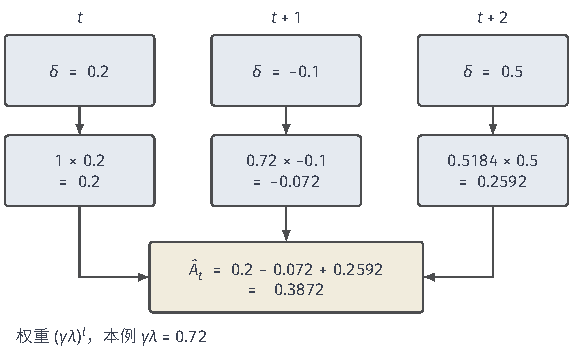
\includegraphics[width=96.961mm]{figures/10-reinforcement-learning/01-problems-and-solving/tikz/rl-learning-gae.pdf}
  \caption{GAE的几何加权。每列是一项TD误差及其对当前优势的贡献；数值是人工指定的三步算例，不是实验学习曲线。}
  \label{fig:rl-learning-gae}
\end{figure}

若评论家等于$V^\pi$，后继TD误差在其动作抽样前历史下均值为0；因此在同策略条件下，对任意$\lambda$，上式给定$(s_t,a_t)$的条件均值均为$A^\pi(s_t,a_t)$。近似评论家则不同。令$e=V_{\bm w}-V^\pi$，在无限折扣和有界误差下，近似GAE相对精确GAE的条件均值变化为
\[
  -e(s_t)+
  \gamma(1-\lambda)\,
  \mathbb E\left[
     \sum_{l=1}^{\infty}(\gamma\lambda)^{l-1}e(s_{t+l})
        \,\middle|\,s_t,a_t\right].
\]
第一项仍是状态基线，乘得分函数后均值为0；第二项通常依赖所选动作，会改变策略更新。$\lambda=1$且完整终止回报可用时，这个自举误差项消失；若仅有截断片段，还留有末端价值误差。表\ref{tab:rl-learning-baseline-bootstrap}将两种评论家用途并排，避免把控制变量的无偏结论错误搬到所有自举目标上\scite{rl3-schulman2016gae}

\begin{table*}[t]
  \centering
  \small
  \begin{tabularx}{\linewidth}{>{\raggedright\arraybackslash}p{30mm} >{\raggedright\arraybackslash}X >{\raggedright\arraybackslash}X}
    \toprule
    评论家的位置 & 估计示例 & 偏差和方差应怎样判断 \\
    \midrule
    状态基线 & 完整$G_t-V_{\bm w}(s_t)$ & 动作抽样前固定即可保持期望；误差影响方差，不保证一定降方差 \\
    未来回报替代 & $r_t+\gamma V_{\bm w}(s_{t+1})-V_{\bm w}(s_t)$ & 后继误差可随动作变化，通常产生自举偏差 \\
    多步混合 & 式\eqref{eq:rl-learning-gae} & $\lambda$和片段长度共同控制自举依赖与随机回报范围 \\
    同批拟合再复用 & 用该动作的回报训练基线并立即扣减 & 必须重新检查条件独立、旧策略比率与重复优化造成的分布变化 \\
    \bottomrule
  \end{tabularx}
  \caption{减去一个数，与用一个数替代尚未观察的未来，是不同操作。}
  \label{tab:rl-learning-baseline-bootstrap}
\end{table*}

% Outline: 3.3.3
\subsection{自然梯度、信赖域与近端更新}
\label{sec:rl-learning-trust-region}

梯度给出方向，步长还需反映动作分布会改变多少。参数距离本身不能提供统一尺度：二动作策略写成$p=\sigma(\theta)$时，$\theta$从0增至$0.1$，$p$约增至$0.5250$；同一策略族改用$\phi=10\theta$，让$\phi$增加$0.1$，$p$却只增至约$0.5025$。相同坐标步长产生了不同的行为变化，因此需要直接用新旧动作分布的差异衡量更新。

令旧参数为$\bm\theta$、候选新参数为$\bm\theta+\bm\Delta$。我们用KL散度比较每个状态的新旧动作分布，并按旧策略占用分布平均，使本次局部比较的状态权重固定。设$S$和合法动作集有限，旧占用$d^\pi$在本次比较中固定，各合法动作概率在开参数邻域内严格为正且二阶连续可微。概率归一化使KL在$\bm\Delta=0$处的一阶项为0，二阶展开为
\begin{align}
  \mathbb E_{d^\pi}\!
    \left[D_{\mathrm{KL}}
       (\pi_{\bm\theta}(\cdot\mid s)
           \Vert\pi_{\bm\theta+\bm\Delta}(\cdot\mid s))\right]
    &=\tfrac12\bm\Delta^\top\bm F\bm\Delta
         +o(\lVert\bm\Delta\rVert^2), \notag\\
  \bm F&=\mathbb E_{d^\pi,\pi}[\bm z\bm z^\top].
  \label{eq:rl-learning-fisher}
\end{align}
一次项因概率归一化而消失；二次项$\bm F$是Fisher信息矩阵，衡量参数变化在动作分布中留下多大痕迹。\term{自然梯度}用这个局部度量而不是坐标长度比较方向。设$\bm g=\nabla J$在有效子空间内非零、$\bm F$在该子空间正定且$\delta>0$，则
\[
  \argmax_{\bm\Delta:\,\bm\Delta^\top\bm F\bm\Delta/2\leq\delta}
       \bm g^\top\bm\Delta
     =
     \sqrt{\frac{2\delta}{\bm g^\top\bm F^{-1}\bm g}}\,
       \bm F^{-1}\bm g.
\]
若$\bm g=\bm0$，局部线性目标没有偏好的上升方向，可取零步；上述归一化公式不适用。若参数冗余导致$\bm F$奇异，应限制到可辨识子空间、使用伪逆，或明确采用$\bm F+\xi\bm I$的阻尼近似。自然梯度的坐标不变性是局部几何性质，不是任意有限步长的回报保证\scite{rl3-kakade2002natural}

自然梯度的约束可以看成给行为变化设置预算。普通梯度在一个参数欧氏球内寻找回报线性近似最大的方向；这里改用$\bm\Delta^\top\bm F\bm\Delta/2\leq\delta$这个椭球，让同样的KL预算可以在不敏感的参数方向走得远一些，在很敏感的方向走得近一些。解椭球内的线性最大化，才得到$\bm F^{-1}\bm g$，而不是因为矩阵可逆就任意将梯度乘一个逆矩阵。它只解释一次局部选择，实际有限步仍要核对动作分布和回报。

局部分布距离说明如何计量一步，却还没有保证回报会上升。要判断改进，需将新策略的回报差写成可评价的优势。下面的恒等式表明：应平均的是新策略实际访问状态上的旧策略优势，不能任意用旧策略轨迹的抽样分布替换。

\begin{theorem}[折扣性能差恒等式]
  \label{thm:rl-learning-performance-difference}
  设$S$有限，各非终止状态的合法动作集有限且非空，奖励有界，$0\leq\gamma<1$。两个平稳策略$\pi,\pi'$使用同一环境核和同一初始分布$\mu_0$，$d^{\pi'}$为其归一化折扣占用分布，$A^\pi=Q^\pi-V^\pi$。则
  \begin{equation}
    J(\pi')-J(\pi)
       =\frac{1}{1-\gamma}
          \mathbb E_{s\sim d^{\pi'},\,a\sim\pi'}[A^\pi(s,a)].
    \label{eq:rl-learning-performance-difference}
  \end{equation}
\end{theorem}
\begin{proof}
  沿$\pi'$的轨迹，条件期望给出
  $A^\pi(s_t,a_t)
    =\mathbb E[r_t+\gamma V^\pi(s_{t+1})-V^\pi(s_t)
                \mid s_t,a_t]$。乘$\gamma^t$并求和到$n-1$，
  \[
    \mathbb E_{\pi'}\sum_{t=0}^{n-1}\gamma^t A^\pi(s_t,a_t)
      =\mathbb E_{\pi'}\sum_{t=0}^{n-1}\gamma^t r_t
         -\mathbb E_{\mu_0}V^\pi(s_0)
         +\gamma^n\mathbb E_{\pi'}V^\pi(s_n).
  \]
  $V^\pi$有界使尾项趋于0，前两项趋于$J(\pi')-J(\pi)$。按归一化占用分布的定义，左边极限等于
  $(1-\gamma)^{-1}\mathbb E_{d^{\pi'},\pi'}A^\pi$。
\end{proof}

更新前尚未收集新策略轨迹，直接计算$d^{\pi'}$下的优势仍有困难。用$d^\pi$替代它，就得到一个可由旧策略轨迹样本估计的局部代理目标；代理提高到什么程度能支持真实改进，还要控制这项替代误差。若连动作也用旧策略样本估计，还需$\pi'(\cdot\mid s)\ll\pi(\cdot\mid s)$，即新策略所选动作在旧策略下有正概率。此时动作比率给出
\[
  \mathcal L_\pi(\pi')
    =J(\pi)+\frac1{1-\gamma}
         \mathbb E_{d^\pi,\,a\sim\pi}
           \left[\frac{\pi'(a\mid s)}{\pi(a\mid s)}
                         A^\pi(s,a)\right].
\]
动作比率校正了同一状态的动作分布，却没有校正状态访问分布。要界住这项变化，使用总变差（total variation, TV）：对离散动作分布$p,q$，
$\operatorname{TV}(p,q)=\tfrac12\sum_a|p(a)-q(a)|
=\tfrac12\lVert p-q\rVert_1$，
其中动作在同一合法域上比较。它也等于$\sup_B|p(B)-q(B)|$，即允许动作事件$B$上概率差的最大值；这个事件定义同样适用于连续分布。令
$\eta=\max_s\operatorname{TV}(\pi'(\cdot\mid s),\pi(\cdot\mid s))$、
$\epsilon_A=\max_{s,a}|A^\pi(s,a)|$。同一转移核按两份动作分布混合时，不放大其$L^1$差，故单步状态转移差至多为$2\eta$；再将占用流方程中的后续传播按折扣累加，可得
$\lVert d^{\pi'}-d^\pi\rVert_1\leq2\gamma\eta/(1-\gamma)$；
又因$\mathbb E_\pi A^\pi=0$，
$|\mathbb E_{\pi'}A^\pi(s,\cdot)|\leq2\epsilon_A\eta$。两式相乘得到
\begin{equation}
  J(\pi')\geq\mathcal L_\pi(\pi')
       -\frac{4\gamma\epsilon_A}{(1-\gamma)^2}\eta^2 .
  \label{eq:rl-learning-trpo-bound}
\end{equation}
这里$\eta$取全部状态上动作分布总变差的最大值，因为少见状态的策略变化也可能改变后续可达区域；仅按旧访问分布平均，可能漏掉这种变化。由Pinsker不等式，可进一步用最大状态KL控制$\eta^2$。因此，下界要求的不只是提高旧策略轨迹样本上的代理，还要限制所有状态的新旧策略差异，使状态分布替代的损失不足以抵消提升。

信赖域策略优化（trust region policy optimization, TRPO）的理论分析从此类下界出发，实践实现则用样本平均KL约束、共轭梯度近似Fisher逆乘积和回溯线搜索，以有限计算求一个局部步。平均KL不控制所有少见状态，估计优势也不等于真实优势，因此“精确下界提高”与“实践TRPO更新”不能无条件互换。兼容函数逼近给出了另一条严格但受限的连接：若评论家为
$f_{\bm w}(s,a)=\bm z(s,a)^\top\bm w$，并在同一$d^\pi\pi$下精确最小化
$\mathbb E[(Q^\pi-b(s)-f_{\bm w})^2]$，
正规方程给出$\mathbb E[\bm z(Q^\pi-b-f_{\bm w})]=0$，从而
$\nabla J=\bm F\bm w/(1-\gamma)$。这要求特征兼容、正确加权和评价解足够准确，不是任意价值网络都保留梯度方向\scite{rl3-schulman2015trpo,rl3-agarwal2021policygradient}

TRPO的约束求解需要额外计算。近端策略优化（proximal policy optimization, PPO）改为优化一个可用于小批量更新的代理，限制过度改变动作概率后还能从同一样本获取多少收益。记旧策略为$\pi_{\mathrm{old}}$，
$q_t(\bm\theta)=\pi_{\bm\theta}(a_t\mid s_t)/
\pi_{\mathrm{old}}(a_t\mid s_t)$，优势在本轮优化中固定。

概率比$q_t$先回答这条旧样本在新策略下应占多少动作权重。例如旧概率为$0.2$，新概率为$0.3$，比率为$1.5$。若优势为正，这份代理鼓励继续增大它；但旧样本没有验证新策略大幅改变后会访问哪里。裁剪目标因此让这条样本在有利方向上的收益到阈值后停止增长，减少继续靠同一条证据推动过大变化的动机。它裁剪的是目标贡献，参数仍由全部样本共同更新。PPO-Clip据此最大化
\begin{equation}
  L^{\mathrm{clip}}(\bm\theta)=
    \widehat{\mathbb E}_t
      \left[\min\left\{q_t\widehat A_t,\,
        \operatorname{clip}(q_t,1-\varepsilon,1+\varepsilon)
                      \widehat A_t\right\}\right].
  \label{eq:rl-learning-ppo-clip}
\end{equation}
这里$\widehat{\mathbb E}_t$使用明确选定的批次权重；若要对应前述折扣代理，权重应匹配$d^{\pi_{\mathrm{old}}}$，均匀抽时间步未必满足。内部最小值是在未裁剪和裁剪后的两项贡献中取较小者，使过大的有利概率变化不再增加代理收益：$\widehat A_t>0$时，$q_t>1+\varepsilon$进入平坦区；$\widehat A_t<0$时，$q_t<1-\varepsilon$进入平坦区。反方向变化仍受惩罚。外层则对策略参数最大化这个批次目标。图\ref{fig:rl-learning-policy-geometry}展示两种优势符号下的曲线，并与参数化例子对照。

\begin{figure*}[t]
  \centering
  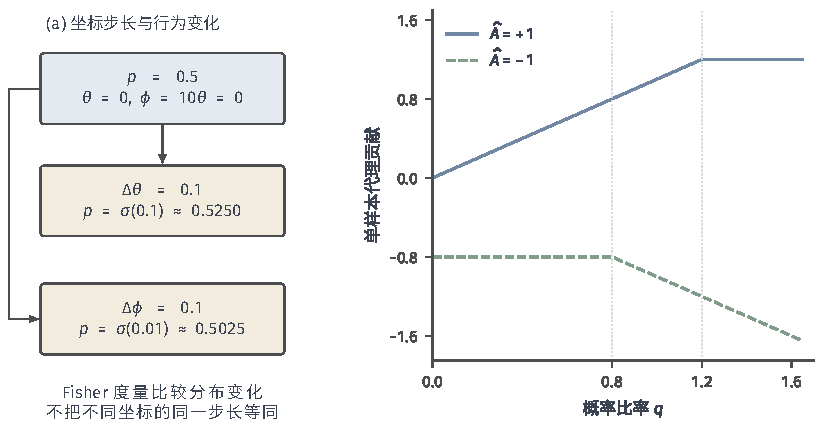
\includegraphics[width=139.587mm]{figures/10-reinforcement-learning/01-problems-and-solving/tikz/rl-learning-policy-geometry.pdf}
  \caption{参数距离、分布距离与PPO裁剪。左侧为同一Bernoulli策略的两种坐标；右侧为$\varepsilon=0.2$、$\widehat A=\pm1$时式\eqref{eq:rl-learning-ppo-clip}的解析折线，裁剪后的平坦区不表示概率比被硬性截住。}
  \label{fig:rl-learning-policy-geometry}
\end{figure*}

例如正优势为1、概率比从1.2变到1.5，单样本贡献仍为1.2；但共享参数受其他样本影响，仍可能继续推动这个比率。PPO-KL改用
$\widehat{\mathbb E}[q_t\widehat A_t]
-\eta_{\mathrm{KL}}\widehat{\mathbb E}_sD_{\mathrm{KL}}
(\pi_{\mathrm{old}}\Vert\pi_{\bm\theta})$
并调节惩罚系数，两者都需要监控实际策略变化。算法\ref{alg:rl-learning-ppo}给出一次完整的交互采样与训练样本复用循环；工程上常加熵项、优势标准化、梯度裁剪与KL提前停止，应分别记录，不能混作裁剪目标的数学性质\scite{rl3-schulman2017ppo}

\begin{algorithm}[一轮PPO-Clip：采样、固定目标与近端优化]
  \label{alg:rl-learning-ppo}
  \begin{algorithmic}[1]
    \State 保存$\bm\theta_{\mathrm{old}}\gets\bm\theta$，冻结旧策略与本轮用于估计优势的评论家。
    \State 用$\pi_{\mathrm{old}}$收集片段，记录状态、动作、$r_t$、真实终止标记、截断标记和旧对数概率。
    \State 真实终止处置末端价值为0；非终止片段边界使用冻结评论家的末端预测。
    \State 从后向前计算式\eqref{eq:rl-learning-gae}，固定$\widehat A_t$与价值目标$\widehat R_t=\widehat A_t+V_{\mathrm{old}}(s_t)$。
    \For{预先指定的$E$轮小批量优化}
      \State 从本轮旧策略采集的训练片段取批次，按已声明权重计算$q_t$与$L^{\mathrm{clip}}$。
      \State 行动者对$L^{\mathrm{clip}}$做梯度上升；评论家对$(V_{\bm w}(s_t)-\widehat R_t)^2$做下降。
      \State 测量旧新策略KL；若采用提前停止规则且超过阈值，停止本轮行动者更新。
    \EndFor
    \State 丢弃本轮作为近端优化依据的旧轨迹批次，使用新策略开始下一轮真实采样。
  \end{algorithmic}
\end{algorithm}

多轮优化复用的是同一个旧分布上的代理，不是每轮都重新获得同策略无偏梯度。理论单调改进是关于特定精确下界和约束的结论；局部平稳性是优化算法的另一类结论；表格softmax等特殊参数化下的全局分析又要求另外的条件。一般神经网络PPO不能从名称中的“近端”继承这三种保证。

\paragraph{小梯度与精确表格保证}
\label{sec:rl-learning-tabular-policy-optimization}
即使梯度完全准确，它很小也未必说明策略已经近优。另设一个单步两动作任务，好动作奖励1、坏动作奖励0，以$p=\sigma(\theta)$表示好动作概率，则$J(\theta)=p$、$J'(\theta)=p(1-p)$。当$p=10^{-6}$时，梯度约为$10^{-6}$，策略离最优回报却仍差$1-10^{-6}$。梯度被罕见动作的概率压小了；多步任务中，很少访问关键状态也会压小相应参数的梯度。因此，普通参数梯度的长度不能单独作为策略损失证书。

自然策略梯度（natural policy gradient, NPG）用Fisher几何调整这些方向的尺度。单步例的Fisher信息为$p(1-p)$，故其逆乘精确梯度得到方向1，而不是随$p$一同趋近零。要把这种局部解释连到一般MDP中的正面结论，可以采用完全表格化、每轮精确评价的设定。以下结论固定同一个初始分布来计算梯度和比较性能，不使用回放分布替代。

\begin{theorem}[精确表格自然策略梯度的全局进展]
  \label{thm:rl-learning-tabular-npg}
  设$S$为非空有限状态集，所有状态共享非空有限动作集$\mathsf A$，$n_A=|\mathsf A|$，环境核时间齐次，奖励为确定性函数$R(s,a)\in[0,1]$，且$0<\gamma<1$。固定初始分布$\mu_0$，并只保留从$\mu_0$出发在某个合法策略下可达的状态，$\pi^*$为该MDP的最优平稳策略。令
  $J(\pi)=\mathbb E_{s_0\sim\mu_0}V^\pi(s_0)$，
  策略按独立状态动作参数作softmax参数化：
  $\pi_{\bm\theta}(a\mid s)=
  e^{\theta_{s,a}}/\sum_b e^{\theta_{s,b}}$。
  记$\pi^{(k)}=\pi_{\bm\theta^{(k)}}$。从$\bm\theta^{(0)}=\bm0$开始，取任意固定步长$\eta>0$。每轮精确计算当前策略的价值、优势、梯度和式\eqref{eq:rl-learning-fisher}中按$d^{\pi_{\bm\theta}}$加权的Fisher矩阵$\bm F(\bm\theta)$，并更新
  $\bm\theta^{(k+1)}=\bm\theta^{(k)}+
  \eta\bm F(\bm\theta^{(k)})^\dagger
          \nabla_{\bm\theta}J(\pi_{\bm\theta})$，其中导数在$\bm\theta^{(k)}$处计算。
  这里$\dagger$为Moore--Penrose伪逆。其诱导策略满足
  \begin{equation}
    \begin{aligned}
    \pi^{(k+1)}(a\mid s)&=
    \frac{\pi^{(k)}(a\mid s)
      \exp\!\left(\eta A^{\pi^{(k)}}(s,a)/(1-\gamma)\right)}
    {Z_k(s)},\\
    Z_k(s)&=\sum_b\pi^{(k)}(b\mid s)
      \exp\!\left(\eta A^{\pi^{(k)}}(s,b)/(1-\gamma)\right),
    \end{aligned}
    \label{eq:rl-learning-tabular-npg-step}
  \end{equation}
  且对每个整数$k\geq1$，
  \begin{equation}
    J(\pi^*)-J(\pi^{(k)})
       \leq\frac{\log n_A}{\eta k}
            +\frac{1}{(1-\gamma)^2k}.
    \label{eq:rl-learning-tabular-npg-rate}
  \end{equation}
\end{theorem}

表格softmax的精确梯度中含有
$d^\pi(s)\pi(a\mid s)A^\pi(s,a)/(1-\gamma)$。
Fisher伪逆在可辨识方向上抵消访问和动作概率带来的尺度，得到式\eqref{eq:rl-learning-tabular-npg-step}；softmax对同一状态的全部参数加相同常数不改变策略，所以使用伪逆不要求冗余参数下的Fisher可逆。在动作分布中，这相当于以旧策略作参考，按当前优势指数加权；第\ref{sec:rl-learning-regularized-search}节将从KL正则的局部优化解释这种形式。

这一更新的进展可以由两个有限量控制。旧策略的平均优势为0，指数的凸性给出$\log Z_k(s)\geq0$；新策略的平均优势则为
$\mathbb E_{\pi^{(k+1)}}A^{\pi^{(k)}}
=(1-\gamma)[D_{\mathrm{KL}}(\pi^{(k+1)}\Vert\pi^{(k)})+\log Z_k(s)]/\eta\geq0$。
性能差恒等式因此给出逐状态价值不下降。对固定最优策略$\pi^*$，更新式还给出
\[
 \frac{\eta}{1-\gamma}
       \mathbb E_{a\sim\pi^*}A^{\pi^{(k)}}(s,a)
 =D_{\mathrm{KL}}(\pi^*\Vert\pi^{(k)})
  -D_{\mathrm{KL}}(\pi^*\Vert\pi^{(k+1)})+\log Z_k(s),
\]
其中各动作分布都条件于同一$s$。按最优策略占用平均并对轮次求和，前两项望远镜相消；均匀初值使剩余初始KL不超过$\log n_A$。从$s$出发的新策略折扣占用在$s$至少有初始质量$1-\gamma$，结合刚才的非负平均优势，又有
$\log Z_k(s)\leq
\eta[V^{\pi^{(k+1)}}(s)-V^{\pi^{(k)}}(s)]/(1-\gamma)$。
故归一化项也可按轮次累加为价值增长，而$[0,1]$奖励使价值范围至多为$1/(1-\gamma)$。再用最后一轮的损失不超过各轮平均，便得到式\eqref{eq:rl-learning-tabular-npg-rate}。该定理及完整分析见Agarwal等的上述研究。

这给出了参数目标虽非凹、特定策略更新仍能趋近全局最优的实例。式中的$k$计精确优化轮次：每轮仍须取得精确价值与梯度，不能将$k$当作真实交互样本数。函数逼近、抽样误差、不同初始分布和PPO裁剪改变了推导条件，需要分别重新控制；Fisher几何本身没有消除这些困难。

% Outline: 3.3.4
\subsection{行动者—评论家的评价—改进耦合}
\label{sec:rl-learning-actor-critic}

前面已用价值基线和优势帮助计算策略更新；实际训练还需要随策略变化不断重学这些评价量。\term{行动者—评论家}（actor--critic）将两个过程耦合：行动者是产生动作的参数策略，评论家是为其更新估计价值或优势的函数。最终目标仍是改进策略，而不是分别追求两个不相关的数值。行动者改变后，评论家的目标策略及后续样本分布也改变，因此必须检查两个更新能否相互跟踪。

对同策略的一步经验，先用奖励和后继估值构造TD误差；评论家据此修正当前价值，行动者则把这个误差当作本次动作的优势。为了与折扣起点目标一致，行动者贡献仍保留$\gamma^t$。一种最简单的联合更新为
\begin{align}
  \delta_t&=r_t+\gamma(1-z_t)V_{\bm w}(s_{t+1})-V_{\bm w}(s_t),
       \notag\\
  \bm w&\gets\bm w+\alpha_t^V\delta_t\nabla_{\bm w}V_{\bm w}(s_t),
       \notag\\
  \bm\theta&\gets\bm\theta+
       \alpha_t\gamma^t\delta_t
          \nabla_{\bm\theta}\log\pi_{\bm\theta}(a_t\mid s_t).
  \label{eq:rl-learning-one-step-ac}
\end{align}
$z_t$仅表示真实终止；若按$d^\pi$直接抽样状态动作，则可把最后一行改写成含$1/(1-\gamma)$的占用分布梯度口径。这里保留回合时间权重，是为了与本章的$J$一致。评论家采用半梯度，行动者把$\delta_t$当成停止求导的优势估计，两个梯度不能混在一起。多步行动者—评论家用$n$步优势或GAE替换$\delta_t$；资格迹则把更新沿过去状态动作传播。

\begin{example}[同一经验的两种更新]
  \label{ex:rl-learning-actor-critic}
  在基准网格起点$(1,1)$，两个合法意图动作是向右和向上。假设当前评论家估计
  $V(1,1)=0.2$、$V(2,1)=0.5$，策略以
  $p_{\text{右}}=\sigma(\theta)$、$\theta=0$表示，均为本次手算指定的初值。第一步选右且实际到达$(2,1)$，得到$r_0=-0.04$，于是
  $\delta_0=-0.04+0.9(0.5)-0.2=0.21$。
  取评论家步长$0.1$，表格状态值更新为$0.221$；取行动者步长$0.2$，因
  $\partial_\theta\log p_{\text{右}}=1-p_{\text{右}}=0.5$，
  $\theta$更新为$0.021$，向右概率变为约$0.50525$。前者提高当前状态的估值，后者提高相对于当前基线表现较好的动作概率；两者不在拟合同一个数。
\end{example}

图\ref{fig:rl-learning-actor-critic}中的两条反馈路径解释了耦合来源。评论家的价值估计会改变行动者的训练目标，行动者又会改变评论家以后看见的样本。即使一次评论家回归收敛，也不代表整个反馈过程已经稳定。

\begin{figure*}[t]
  \centering
  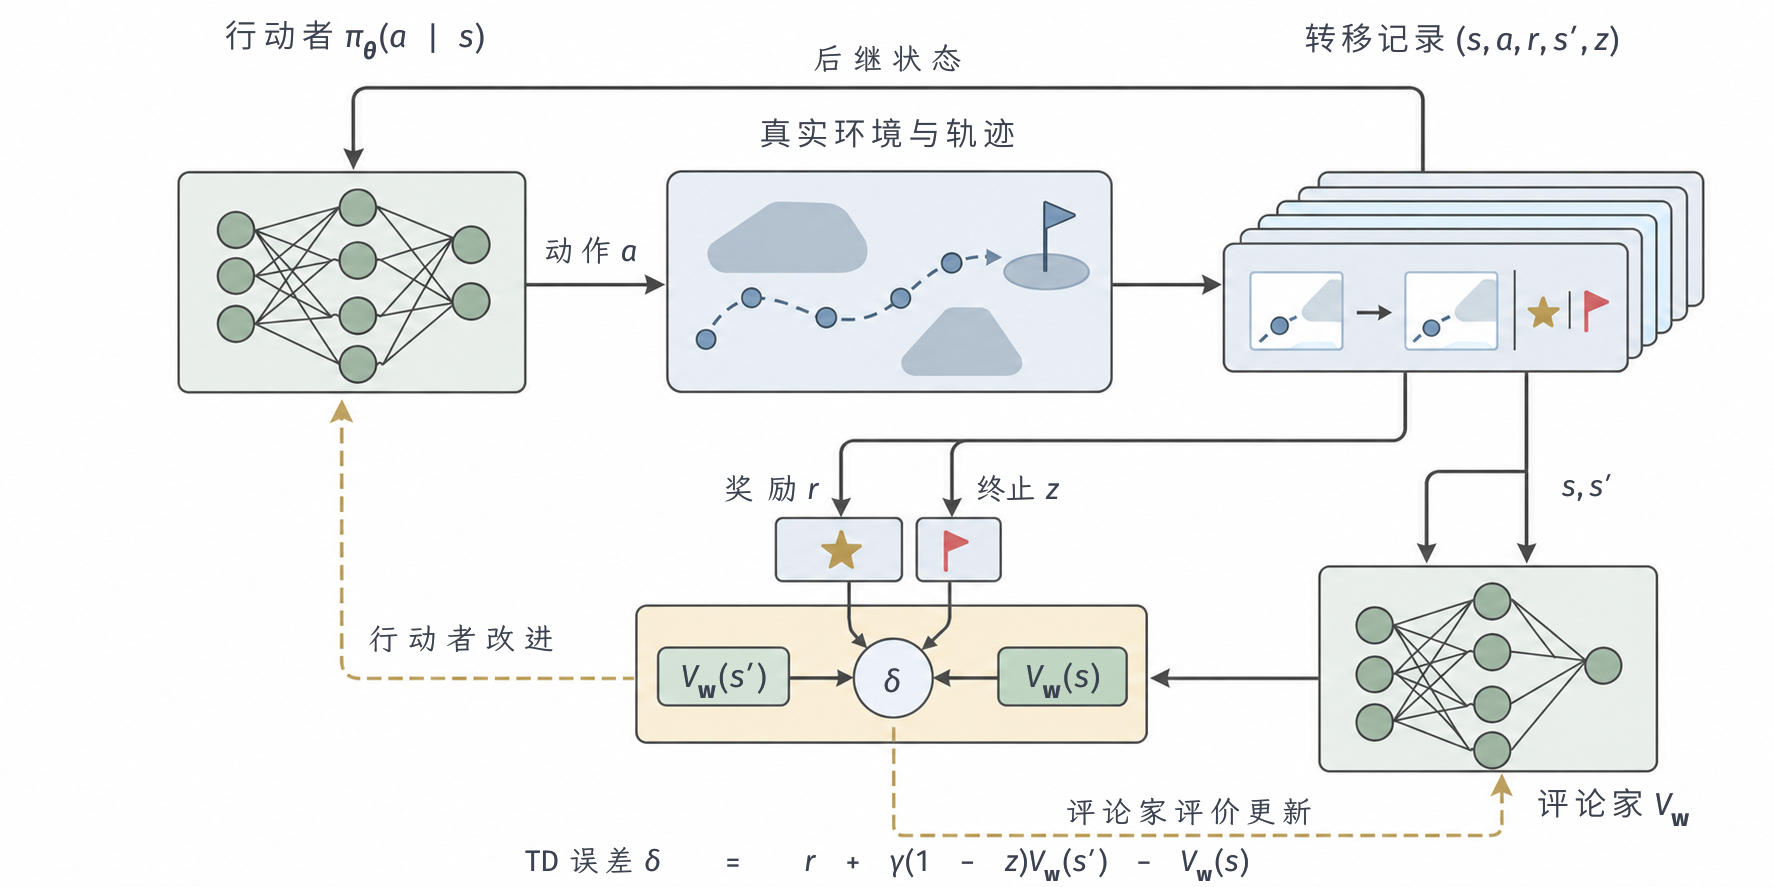
\includegraphics[width=157.400mm]{figures/10-reinforcement-learning/01-problems-and-solving/generated/rl-learning-actor-critic/figure.png}
  \caption{行动者—评论家的共享转移记录与两条更新路径。实线表示采样和价值估计，黄色虚线分别更新行动者与评论家；评论家估计的是价值。轨迹与神经节点仅为机制示意，不表示固定网络结构或轨迹长度。}
  \label{fig:rl-learning-actor-critic}
\end{figure*}

\Needspace{14\baselineskip}
A2C常把多个采样器在同一组参数下收集的短片段同步汇总再更新；A3C则允许采样器异步贡献梯度\scite{rl3-mnih2016asynchronous}
表\ref{tab:rl-learning-ac-interfaces}把这一区别落实到目标对应的轨迹采样条件。异步减少等待，不会让旧参数产生的动作自动变成当前策略动作。

\begin{table*}[t]
  \centering
  \small
  \begin{tabularx}{\linewidth}{>{\raggedright\arraybackslash}p{21mm} >{\raggedright\arraybackslash}X >{\raggedright\arraybackslash}X}
    \toprule
    接口 & 轨迹采样与更新时机 & 需要检查的条件 \\
    \midrule
    一步AC & 一次转移后更新价值与策略 & TD自举误差、步长、样本权重 \\
    A2C & 多环境短片段同步形成一个更新批次 & 批次内策略版本和终止处理一致；并行仅改变采样组织 \\
    A3C & 工作进程使用局部参数采样，异步提交梯度 & 参数滞后与更新冲突；当前全局参数下通常已非严格同策略 \\
    带GAE的AC & 冻结评价器构造片段优势，再更新策略 & $\lambda$、末端自举与估计器是否固定；重复批次优化另需分布处理 \\
    \bottomrule
  \end{tabularx}
  \caption{行动者—评论家的轨迹采样接口。同步、异步与优势长度是可以组合的不同维度。}
  \label{tab:rl-learning-ac-interfaces}
\end{table*}

经典双时间尺度分析让评论家比行动者变化得快。若评论家步长为$\alpha_t^V$、行动者为$\alpha_t$，典型要求为两者的和发散、平方和收敛，并有$\alpha_t/\alpha_t^V\to0$。再加上适用的遍历性、平滑性、参数有界性以及评论家在固定策略下存在稳定且可跟踪的解，快速过程可近似看成已经评价了当前策略，慢速过程才接近一个策略改进常微分方程。线性或兼容评论家等参数化条件决定这个方程是否为真正梯度场；非凸参数化的结果通常也只是局部或驻点性质。固定大步长、任意共享深度网络及不受控参数滞后均不由这条证明路线覆盖\scite{rl3-konda2000actor}

% Outline: 3.3.5
\subsection{连续动作、离策略与最大熵更新}
\label{sec:rl-learning-continuous-soft}

连续动作无法逐个比较，但若评论家能给出动作附近的价值变化，就可以沿价值上升方向调整行动者输出。令确定性行动者为$a=f_{\bm\theta}(s)$，其诱导策略为$\pi_{\bm\theta}$。确定性策略梯度（deterministic policy gradient, DPG）先求$Q$对动作的导数，再通过行动者传到参数；若所需函数可微、导数可积，则
\begin{equation}
  \nabla_{\bm\theta}J
    =\frac1{1-\gamma}
       \mathbb E_{s\sim d^{\pi_{\bm\theta}}}
       \left[
         (\nabla_{\bm\theta}f_{\bm\theta}(s))^\top
         \left.\nabla_a Q^{\pi_{\bm\theta}}(s,a)
                    \right|_{a=f_{\bm\theta}(s)}
       \right].
  \label{eq:rl-learning-dpg}
\end{equation}
行动者沿评论家认为价值上升的动作方向移动，再用链式法则把这个方向传到参数。环境仍不必可微，但评论家的动作导数必须有意义；动作上的函数值误差小，也不保证动作导数准确\scite{rl3-silver2014dpg}

动作方向导数可在一个局部教学评论家上观察。固定状态，令$Q(s,a)=-(a-0.6)^2$、行动者输出$a=\theta$。当前$\theta=0.2$时，$\partial_aQ=0.8$，$\partial_\theta a=1$，参数上升方向就是$0.8$；步长$0.1$使动作变为$0.28$，更靠近评论家给出的峰值。这里无需枚举实数动作，但只有评论家曲线确实反映任务价值时，这个方向才有意义。后文的双评论家和平滑目标都在处理这项依赖。

深度确定性策略梯度（deep deterministic policy gradient, DDPG）把确定性行动者、评论家、经验回放与缓慢跟踪的目标网络组合起来\scite{rl1-lillicrap2016-ddpg}
它用回放中的转移训练记录拟合$Q_{\bm w}$，目标为
$y=r+\gamma(1-z)Q_{\bar{\bm w}}(s',f_{\bar{\bm\theta}}(s'))$，
并用回放状态上的
$\nabla_{\bm\theta}f^\top\nabla_a Q_{\bm w}$
更新行动者。横线表示缓慢移动的目标参数。真实执行常在确定性输出上叠加探索噪声，再投影到动作约束内；探索用的噪声不等于行动者目标本身。

\Needspace{8\baselineskip}
记固定回放状态分布为$\nu$。它可能混合多个历史行为策略，并不一定是某一策略的归一化折扣占用，通常也不同于式\eqref{eq:rl-learning-dpg}中的$d^{\pi_{\bm\theta}}$。若另以该分布为起点定义目标
\[
  J_\nu(\bm\theta)=\mathbb E_{s\sim\nu}V^{\pi_{\bm\theta}}(s),
\]
其精确梯度的状态权重仍是从$\nu$出发、沿当前策略继续访问形成的折扣占用，而不只是$\nu$本身。仅用回放状态的链式乘积，是一个固定状态权重的行动者代理或相应离策略近似；忽略未来访问对参数的依赖，不能被“回放记录可以复用”替代为精确性证明。

双延迟深度确定性策略梯度（twin delayed deep deterministic policy gradient, TD3）在这个接口上处理三类不同误差。双评论家的较小值降低目标过估计，目标动作平滑限制行动者利用极窄的价值尖峰，延迟行动者更新则让评论家先拟合若干批回放记录。其目标可写成
\[
  \widetilde a'
    =\operatorname{proj}_{\mathsf A}
        \bigl(f_{\bar{\bm\theta}}(s')
              +\operatorname{clip}(\bm\epsilon,-c,c)\bigr),
  \qquad
  y=r+\gamma(1-z)\min_{j=1,2}Q_{\bar{\bm w}_j}(s',\widetilde a').
\]
\Needspace{14\baselineskip}
$\bm\epsilon$是人为加入的目标噪声，通常取零均值高斯。TD3的三个部件分别调整目标估值、行动者更新时机和目标动作的局部平均\scite{rl3-fujimoto2018td3}
较小值也可能低估；平滑尺度过大可能抹掉真实的窄最优区域。这些稳定化措施不消除所有评论家误差。

确定性输出通常另加噪声取得探索转移记录。另一种做法把随机性本身纳入策略目标，让高回报动作附近仍保留多个选择。\term{最大熵强化学习}（maximum entropy reinforcement learning）在原回报之外奖励策略熵，即动作分布的分散程度；温度$\alpha>0$决定愿意为这种分散程度付出多少回报。目标为
\begin{equation}
  J_\alpha(\pi)=\mathbb E_\pi\sum_{t\geq0}\gamma^t
      \bigl[r_t-\alpha\log\pi(a_t\mid s_t)\bigr].
  \label{eq:rl-learning-maxent-objective}
\end{equation}
这已经改变优化目标，不只是降低原目标梯度的方差。有限动作下，熵是
$H(p)=-\sum_a p_a\log p_a$；连续动作下使用给定参考测度的密度和微分熵，其数值依赖动作尺度，甚至可以为负。

熵如何改变选择，可以继续看两个动作。确定选择一个动作的熵为0，各以$1/2$选择的熵为$\log2$。若动作评分相差不大，增加一点随机性损失的平均回报较少，却可能得到较多熵奖励；温度$\alpha$就决定这两项如何折算。接下来不是对动作取最大，而是在全部合法动作概率分布中最大化“平均评分加熵”，因此最优解会成为软概率分布。

固定一个状态$s$，令$A_s=\mathsf A(s)$为有限非空的合法动作集，评分$q_a\in\mathbb R$、温度$\alpha>0$均固定。候选是$A_s$上的全部概率分布；熵取$H(p)=-\sum_{a\in A_s}p_a\log p_a$，约定$0\log0=0$。平均评分加熵的最大值及唯一最优分布为
\[
 \begin{aligned}
 \max_{p\in\Delta(A_s)}
   \left\{\sum_{a\in A_s}p_aq_a+\alpha H(p)\right\}
  &=\alpha\log Z,\\
 Z&=\sum_{a\in A_s}e^{q_a/\alpha},\qquad
 p_a^*=\frac{e^{q_a/\alpha}}Z.
 \end{aligned}
\]
这是有限合法动作上的Gibbs变分结果。可直接把局部目标写成$\alpha\log Z-\alpha D_{\mathrm{KL}}(p\Vert p^*)$：KL非负、仅在$p=p^*$时为0，故最优值与唯一性成立。$A_s$有限非空且评分有限保证$0<Z<\infty$和$p_a^*>0$。这个结果用于把动作评分转成软策略改进，不是实际神经行动者一定能精确拟合$p^*$的保证。

例如固定评分为$(0.7,0.4)$，软改进使动作概率之比为$\exp(0.3/\alpha)$。取$\alpha=0.3$，高评分动作概率为$e/(1+e)\approx0.7311$；取$\alpha=0.1$则约为$0.9526$。温度较低时，同一评分差带来更集中的选择。这里的概率直接来自有限动作变分解，不是神经策略一次梯度更新后的精确结果。

固定策略的软价值采用一致的熵位置约定：
\begin{align}
  Q_\alpha^\pi(s,a)
    &=R(s,a)+\gamma\mathbb E[V_\alpha^\pi(s')\mid s,a],
       \notag\\
  V_\alpha^\pi(s)
    &=\mathbb E_{a\sim\pi}
        [Q_\alpha^\pi(s,a)-\alpha\log\pi(a\mid s)].
  \label{eq:rl-learning-soft-bellman}
\end{align}
这里$Q_\alpha^\pi$不含当前动作的熵，$V_\alpha^\pi$含当前策略熵。上面的变分恒等式据此给出软策略改进。连续动作可把求和换为积分，但须满足分区函数有限及相关熵、回报可积；在无界动作空间上，常数$q$的指数函数就不能归一化成密度。

连续动作的Boltzmann分布即密度与指数动作评分成比例的分布，往往难以直接归一化和抽样；软行动者—评论家（soft actor--critic, SAC）改用可训练的参数策略近似软改进。可重参数化指先抽与参数无关的噪声，再通过可微变换生成动作，从而能够沿动作传导评论家梯度。以有界动作为例，
$\bm u=\bm m_{\bm\theta}(s)+\bm\sigma_{\bm\theta}(s)\odot\bm\epsilon$、
$\bm\epsilon\sim\mathcal N(\bm0,\bm I)$、
$a=\tanh\bm u$。
动作归一化到$(-1,1)$时，密度必须包含变换Jacobian：
\[
  \log\pi_{\bm\theta}(a\mid s)
    =\log\mathcal N(\bm u;\bm m_{\bm\theta},
                           \operatorname{diag}\bm\sigma_{\bm\theta}^2)
       -\sum_i\log(1-\tanh^2u_i).
\]
若再缩放到物理动作区间，还需加入该线性变换的对数行列式。漏掉Jacobian会同时改变熵、行动者梯度和温度更新。

重参数化把“抽动作”拆成“抽固定噪声”和“用参数变换噪声”。这样一次已抽取的$\bm\epsilon$可以固定，参数变化仍通过均值、尺度和$\tanh$连续改变动作，评论家的动作导数就能传回策略。密度修正则是另一件事：$\tanh$在靠近边界时压缩区间，把相同概率质量挤到更短的动作区间，密度因而改变。Jacobian项补偿这种区间变形，不能因为动作由网络输出就省去。

动作密度确定后，评论家和行动者在同一批回放状态上使用不同来源的动作求值：评论家评价记录动作，行动者则重新抽取当前策略动作，以提高软价值。采用不单设价值网络的常见SAC版本，在后继状态采样
$a'\sim\pi_{\bm\theta}(\cdot\mid s')$，并记当前状态重采样动作为
$a_{\bm\theta}=f_{\bm\theta}(s,\bm\epsilon)$。回放批次中一次目标和两个损失为
\begin{align}
  y&=r+\gamma(1-z)
       [\min_j Q_{\bar{\bm w}_j}(s',a')
                       -\alpha\log\pi_{\bm\theta}(a'\mid s')],
       \notag\\
  L_Q(\bm w_j)&=\tfrac12\widehat{\mathbb E}_{D}
                           [(Q_{\bm w_j}(s,a)-\operatorname{sg}(y))^2],
       \notag\\
  L_\pi(\bm\theta)&=
       \widehat{\mathbb E}_{s\sim\widehat P_D^S,\,\bm\epsilon}
       [\alpha\log\pi_{\bm\theta}(a_{\bm\theta}\mid s)
        -\min_j Q_{\bm w_j}(s,a_{\bm\theta})].
  \label{eq:rl-learning-sac-losses}
\end{align}
同一组当前评论家参数需要作两次不同求值：评论家损失使用记录动作的$Q_{\bm w_j}(s,a)$，行动者损失使用重新采样动作的$Q_{\bm w_j}(s,a_{\bm\theta})$。更新行动者时，固定$\bm w_j$，但保留第二次求值对动作的导数；更新评论家时，整个$y$停止求导。两次求值共享参数，不代表可以把记录动作的估值直接送入行动者损失。图\ref{fig:rl-learning-sac}将这两个容易混淆的路径分开。表格软策略迭代中精确评价和精确改进的结论，并不能证明这两个近似神经网络损失在任意回放分布下收敛\scite{rl3-haarnoja2018sac}

\begin{figure*}[t]
  \centering
  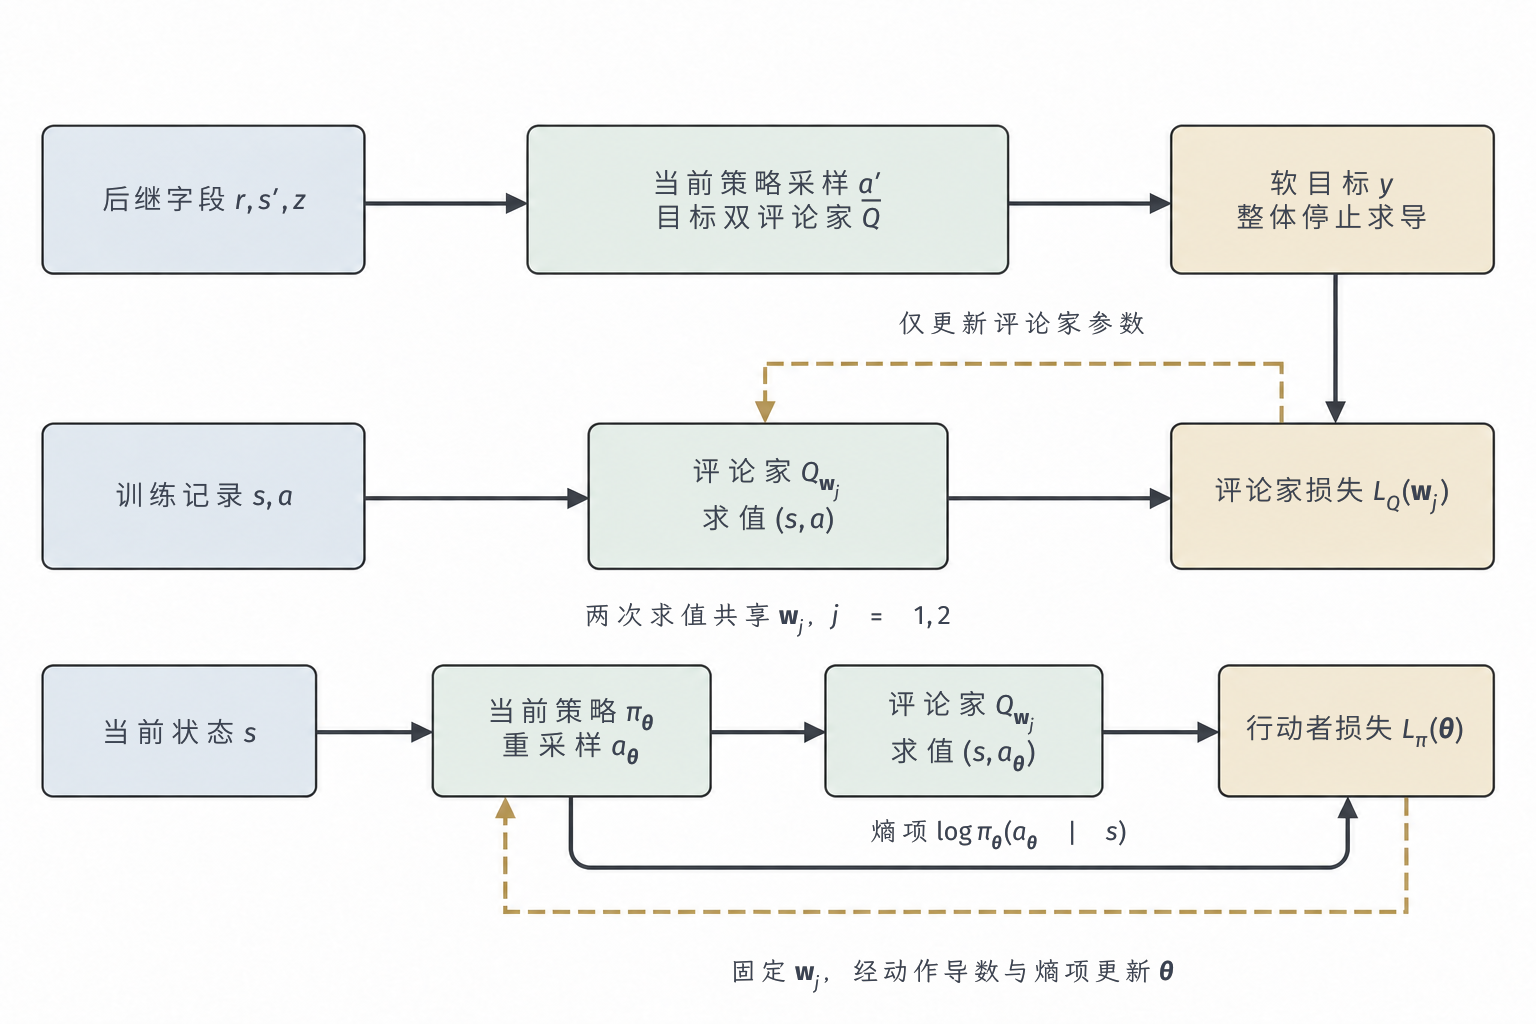
\includegraphics[width=157.400mm]{figures/10-reinforcement-learning/01-problems-and-solving/generated/rl-learning-sac/figure.png}
  \caption{SAC的目标构造、评论家拟合与行动者改进。上排由后继训练字段构造停止求导的软目标；中排用回放记录动作求值并拟合目标；下排在当前状态重新采样策略动作，再调用共享参数的评论家优化行动者。行动者更新固定评论家参数，保留其对动作的导数；目标中的后继动作来自当前策略，软价值由目标评论家计算，整个目标停止求导。}
  \label{fig:rl-learning-sac}
\end{figure*}

温度可以由目标熵$H_0$自动调整。令$\alpha=e^\xi$，对
$L_\alpha(\xi)=
\widehat{\mathbb E}[e^\xi(-\log\pi_{\bm\theta}(a\mid s)-H_0)]$
下降，且在此步固定策略样本和对数密度。当前熵低于目标时梯度为负，$\xi$上升，从而提高探索的熵奖励；高于目标时方向相反。连续动作的$H_0$可以为负，不应把它当成离散动作数的对数。算法\ref{alg:rl-learning-sac}明确了更新顺序；独立价值网络被移除与自动温度来自后续SAC算法版本，应与最初论文的实现区分\scite{rl3-haarnoja2018applications}

\begin{algorithm}[SAC的真实数据与离策略更新循环]
  \label{alg:rl-learning-sac}
  \begin{algorithmic}[1]
    \State 初始化策略、两个评论家、对应目标评论家、温度及真实回放$D$。
    \For{每个真实交互步}
      \State 由当前策略采样动作并执行，记录$(s,a,r,s',z)$；预热阶段可使用指定随机策略。
      \State 将经验写入$D$；真实终止或环境时间上限要求重置时取得新起点，否则转到$s'$。
      \State 仅时间截断仍令$z=0$，记录中的$s'$保留重置前的后继观测。
      \For{预先规定的$U$次梯度更新}
        \State 从$D$抽批次，在后继状态按当前策略采样$a'$，构造停止求导的$y$。
        \State 两个评论家分别最小化$L_Q$，不向目标网络和目标动作反向传播。
        \State 在同批状态重新采样可重参数化动作，固定评论家参数，最小化$L_\pi$。
        \State 若自动调温，固定策略输出并最小化$L_\alpha$。
        \State 目标参数更新为$\bar{\bm w}_j\gets(1-\tau)\bar{\bm w}_j+\tau\bm w_j$。
      \EndFor
    \EndFor
  \end{algorithmic}
\end{algorithm}

例如一条人工经验有$r=0.1$、$\gamma=0.9$、$z=0$，
后继动作的两个目标值为$(0.7,0.9)$，
$\log\pi(a'\mid s')=-0.5$、$\alpha=0.2$，则$y=0.1+0.9(0.7+0.1)=0.82$。
若一个表格评论家当前值为$0.6$，步长$0.1$的一次平方损失更新得到$0.622$。
在当前状态另采一个动作，若$\min Q=0.65$、$\log\pi=-0.8$，其行动者损失样本为$-0.16-0.65=-0.81$；这个数值还不足以决定参数步长，必须通过密度和$Q$的动作导数求梯度。它不等于用记录动作做监督学习。

离策略和近端约束也可以按其他方式组合。表\ref{tab:rl-learning-off-policy-actors}比较四种接口，关注的是概率比在哪个位置校正旧策略轨迹的抽样分布、哪些参数被当作旧策略，而非把分布式采样本身当成学习保证。

这些组合分别针对不同的复用困难。ACER（actor--critic with experience replay）保留截断重要性比之外的补偿，使少抽样动作的贡献不被直接丢掉。IMPALA将采样器与学习器分开，V-trace用来处理两边策略版本的差异。MPO（maximum a posteriori policy optimisation）先在评论家评分下求一份改进的动作分布，再用参数策略拟合这份分布；这里两步的目标和约束不同。APPO（asynchronous proximal policy optimization）则在异步采集的轨迹记录上组合离策略目标与近端代理。下面的表是这些职责的汇总，具体保证仍由校正位置和抽样条件决定。

\begin{table*}[t]
  \centering
  \small
  \begin{tabularx}{\linewidth}{>{\raggedright\arraybackslash}p{17mm} >{\raggedright\arraybackslash}X >{\raggedright\arraybackslash}X}
    \toprule
    方法 & 校正或约束的位置 & 轨迹采样接口与边界 \\
    \midrule
    ACER & 截断重要性比率加偏差校正项，配合Retrace评价及策略变化约束 & 回放与当前采样结合；只截断而丢掉补偿项不是相同估计器 \\
    IMPALA & V-trace校正行为策略与学习器策略差异 & 解耦采样和学习；截断阈值影响评价目标，见前文V-trace \\
    MPO & E步构造受KL约束的动作改进分布，M步在约束下拟合参数策略 & 常用回放状态和评论家；动作改进与状态分布覆盖是不同问题 \\
    APPO & 异步采样下结合V-trace目标与近端概率比代理 & 行为、目标和学习策略可能不同；须报告具体实现的目标同步及比率定义 \\
    \bottomrule
  \end{tabularx}
  \caption{轨迹记录复用、策略滞后和更新约束的几种组合。APPO是实现族名称，不能假定所有版本具有同一估计目标。}
  \label{tab:rl-learning-off-policy-actors}
\end{table*}

\Needspace{24\baselineskip}
ACER的重要性截断补偿需要同时保留被截断部分的期望校正；否则得到的是另一个有偏梯度\scite{rl3-wang2017acer}
Retrace提供评价目标，策略变化约束则限制更新幅度，两者不能替代概率比支持条件。

MPO的受约束动作分布改进与参数拟合分成两步，能分别控制非参数改进和参数投影。回放状态仍来自行为分布，动作分布上的KL约束并不自动解决未覆盖状态的问题\scite{rl3-abdolmaleki2018mpo}

\Needspace{18\baselineskip}
IMPALA已经在离策略评价中出现。APPO的具体工程版本应以使用的实现文档为准\scite{rl3-rllib-appo}
训练报告需要保存版本与配置，不能只写一个缩写就省去旧策略的定义。

% Outline: 3.3.6
\subsection{正则化与无梯度策略搜索}
\label{sec:rl-learning-regularized-search}

熵奖励鼓励保留多个动作，KL约束则限制离开参考行为。固定某状态的动作评分后，可以把两者写成同一个局部选择问题：在合法动作的概率分布中，增大平均评分，同时惩罚相对参考分布的KL。给定$q_a$、$p_a^{\mathrm{ref}}$和$\alpha>0$，考虑
\[
  \max_p\left\{\sum_a p_a q_a
          -\alpha D_{\mathrm{KL}}(p\Vert p^{\mathrm{ref}})\right\}.
\]
在参考分布的正支撑上，对概率归一化约束引入乘子并求导，
$q_a-\alpha(\log(p_a/p_a^{\mathrm{ref}})+1)-\lambda=0$，
从而
\begin{equation}
  p_a^{\mathrm{new}}
     =\frac{p_a^{\mathrm{ref}}e^{q_a/\alpha}}
            {\sum_b p_b^{\mathrm{ref}}e^{q_b/\alpha}}.
  \label{eq:rl-learning-exponential-update}
\end{equation}
参考分布取均匀分布时回到熵正则；取旧策略时得到KL几何下的一步镜像上升。若评分取当前精确优势、$\alpha=(1-\gamma)/\eta$，就得到式\eqref{eq:rl-learning-tabular-npg-step}的表格NPG策略更新；相应全局进展还依赖定理中的精确评价、初始化与共同目标条件。若$p_a^{\mathrm{ref}}=0$，任何给该动作正质量的$p$都会产生无限KL，更新无法重新发现它。这是支持集的限制，不是温度再小就能克服的数值问题。

式\eqref{eq:rl-learning-exponential-update}也说明参考分布的作用。仍取评分$(0.7,0.4)$、$\alpha=0.3$，若旧动作概率为$(0.2,0.8)$，新概率按$(0.2e,0.8)$归一化，高评分动作只增至约$0.4046$；若参考概率均为$1/2$，它会增至约$0.7311$。相同评分在不同参考分布下形成不同更新，因为这里既奖励高评分，也惩罚离开旧行为。这种在分布几何中作局部上升的做法称为镜像上升（mirror ascent）。

图\ref{fig:rl-learning-regularized-search}上半部展示这一局部更新。相似的指数权重也可从概率条件化得到，这一视角称为\term{控制即推断}（control as inference）：把奖励较高的轨迹赋予较大的“最优性”事件概率，再推断条件于该事件的行为。在离散有限时域模型中，设最优性变量的条件概率与$\exp(r_t/\alpha)$成比例，给定动作先验和真实动力学，轨迹后验便按指数回报重加权。不过，随机环境的精确后验还可能偏好幸运转移，而策略无法控制这种运气。要对应可执行控制，需固定变分轨迹族的真实环境核，只优化策略，并说明近似推断范围。因此这个构造可以解释某些熵与KL目标，不能把所有策略算法都视为同一精确后验求解\scite{rl3-levine2018inference}

以上更新需要动作评分或梯度。若策略包含不可微程序，或者只能在整回合结束后查询回报，可以改为试验多组策略参数。\term{交叉熵方法}（cross-entropy method, CEM）维护参数搜索分布，保留估计回报较高的一部分候选作为精英，再拟合这些候选以改变下一轮试验范围。若搜索分布为高斯，第$k$轮采样
$\bm\theta_i\sim\mathcal N(\bm m^{(k)},\bm C^{(k)})$，按估计回报选出精英集合$\mathcal E$，则未平滑更新为
\[
  \bm m^{(k+1)}
       =\frac1{|\mathcal E|}\sum_{i\in\mathcal E}\bm\theta_i,
  \qquad
  \bm C^{(k+1)}
       =\frac1{|\mathcal E|}\sum_{i\in\mathcal E}
       (\bm\theta_i-\bm m^{(k+1)})
       (\bm\theta_i-\bm m^{(k+1)})^\top.
\]
实际可设置最小协方差或平滑更新，防止过早塌缩。图\ref{fig:rl-learning-regularized-search}下半部使用独立一维教学回报
$F(\theta)=-(\theta-1)^2$：四个候选为$(-1,0,1,2)$，得分$(-4,-1,0,-1)$；预先约定并列时选较小参数，保留两名精英$(0,1)$，得到新均值$0.5$、最大似然方差$0.25$。这里的候选与得分都是人工给定，不是一次真实训练的测量结果\scite{rl3-rubinstein1999crossentropy}

\begin{figure*}[t]
  \centering
  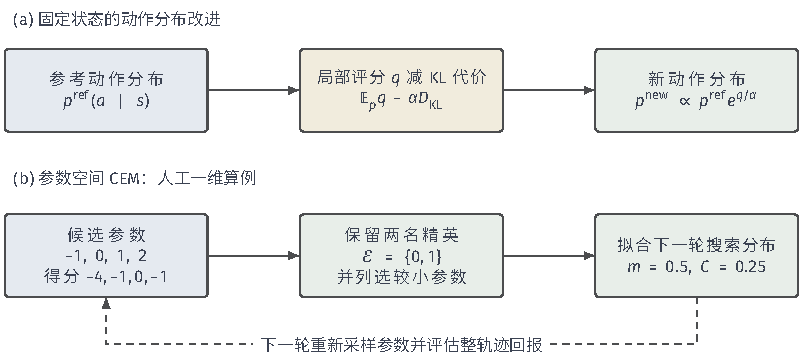
\includegraphics[width=135.961mm]{figures/10-reinforcement-learning/01-problems-and-solving/tikz/rl-learning-regularized-search.pdf}
  \caption{两类策略搜索分布。上排在固定状态对动作分布做正则化改进，下排在参数空间选择精英并拟合搜索分布；动作概率与参数采样概率不能混为一谈。}
  \label{fig:rl-learning-regularized-search}
\end{figure*}

交叉熵方法的名称来自拟合搜索分布：把精英候选看成经验目标分布，提高搜索分布在这些候选上的平均对数密度，等价于减少相应交叉熵。高斯情况下得到精英均值与协方差。这里被拟合的是“下一轮试哪些参数”的分布，不是状态下的动作策略；最终仍需从候选或搜索结果中确定一份可执行策略。

CEM只用精英筛选和拟合改变搜索分布，进化策略（evolution strategies, ES）还可以用参数扰动与回报的关系估计方向。先将原目标在高斯邻域内平均，定义
$F_\sigma(\bm\theta)=
\mathbb E_{\bm\epsilon\sim\mathcal N(\bm0,\bm I)}
J(\bm\theta+\sigma\bm\epsilon)$，则在可积条件下
\[
  \nabla F_\sigma(\bm\theta)
    =\frac1{\sigma}\mathbb E[J(\bm\theta+\sigma\bm\epsilon)\bm\epsilon].
\]
使用成对扰动可估计为
$(2N\sigma)^{-1}\sum_i
[\,\widehat J(\bm\theta+\sigma\bm\epsilon_i)
-\widehat J(\bm\theta-\sigma\bm\epsilon_i)\,]\bm\epsilon_i$。
\Needspace{16\baselineskip}
它求的是平滑后的参数目标，$\sigma$既决定探索范围也改变平滑偏差\scite{rl3-salimans2017es}

\Needspace{16\baselineskip}
CMA-ES进一步用选择结果及跨轮演化路径更新协方差和全局步长，使参数试验适应不同方向的尺度；并非仅把CEM的样本协方差换个名字\scite{rl3-hansen2001cma}

参数空间探索让一整段行为保持同一次参数扰动，可能形成时间一致的探索；每步动作噪声则在同一策略附近不断改变局部控制。前者不能免费绕过长时程困难：每组参数仍需足够回合才能辨认真实回报，高维全协方差要存储和估计二次数量的参数，排名还会被回报噪声改变。是否值得使用，应比较总真实交互、可并行程度、策略可微性和搜索维度，而不是只比较一次更新公式的长度。

% Outline: 3.4
\section{基于模型的价值学习}
\label{sec:rl-learning-model-value}

回放可以重复使用记录，却不能直接回答某个未记录动作的后果。学习环境模型把已见经验拟合成可查询的后继和奖励预测器，用它补充价值更新或当前动作比较。模型预测有两种直接用途：Dyna生成模拟经验后更新动作价值；MPC预测当前候选轨迹的回报，选出计划后只执行首动作。MPC未必训练独立价值函数，但动作仍由预计回报比较产生。用模型训练跨状态共享的参数策略，则能把部分搜索计算转移到训练阶段，供执行时直接调用。

% Outline: 3.4.1
\subsection{环境模型的表示与不确定性}
\label{sec:rl-learning-model-representation}

在基准网格的$(3,2)$执行向右，后继位置可能为$(4,2)$、$(3,3)$或$(3,1)$，概率分别是$0.8,0.1,0.1$。若把坐标当连续量并最小化平方预测误差，最优输出是条件均值$(3.8,2)$，但网格没有这个状态。平均位置既不能告诉规划器滑移会通往哪里，也不能直接代入只在合法格点上定义的价值函数。预测损失选错对象，甚至会使一个统计上正确的条件均值不适合控制。

对这个网格，合适的模型应给每个合法落点分配概率。假设在同一状态动作下观察到10次结果，其中8次到$(4,2)$、另外两个落点各1次，经验概率就是$(0.8,0.1,0.1)$。这些是教学计数，恰好与真实概率一致；实际有限样本未必如此。给定$(s,a)$后输出一份后继概率分布，就是转移概率核在这里的含义；“核”强调每个输入各有一份分布，不要求它是某个核函数。

拟合概率也需要选择准则。将每条记录的已发生后继代入预测分布，所有记录的概率相乘形成似然；取负对数后乘积变成可累加的损失。上述计数下，候选概率$(p_1,p_2,p_3)$的平均损失为$-[8\log p_1+\log p_2+\log p_3]/10$。在概率非负且和为1的约束下，最小化它得到相应经验频率。后面的神经模型保留这一“给实际结果较高概率”的原则，只是不同状态动作会共享参数。

\begin{definition}[学得环境模型的预测对象]
  \label{def:rl-learning-learned-model}
  设$S$与$\mathsf A$为可测空间，合法状态动作域为$X=\{(s,a):s\in S,\ a\in\mathsf A(s)\}$，并在$X$上约定可测结构。\term{确定性动力学模型}的候选是可测映射$\widehat f_{\bm\phi}:X\to S$；\term{随机动力学模型}的候选是从$X$到$S$的概率核$\widehat T_{\bm\phi}(\cdot\mid s,a)$。给定训练记录和学习规则后得到的具体映射或核，称为学得的动力学模型。贝叶斯方法在参数或函数上保持给定先验与似然产生的后验，并对该后验积分得到预测；集成方法保留若干分别拟合的预测器，例如通过重采样训练记录和随机初始化得到。两者描述参数不确定性的处理方式，不与确定性或随机后继预测互斥。

  奖励均值模型为可测函数$\widehat R:X\to\mathbb R$，继续概率模型为可测函数$\widehat c(s,a,s')\in[0,1]$。也可学习$(s',r,c)$的联合概率核，以保留奖励、后继与继续事件之间的相关性。
\end{definition}
这些预测量需要从真实记录中学习，而不是按控制回报直接拟合。令$c_t=0$表示执行$a_t$后真正终止，$c_t=1$表示继续。对具备随机后继、条件奖励和继续预测的模型，可以最小化记录中三个结果的负对数似然；期望按真实回放记录的经验抽样律$\widehat P_{D_{\mathrm{real}}}$取，候选变量是模型参数$\bm\phi$：有限状态时，转移核可用条件质量函数表示；连续状态时，须先选定参考测度$\nu$，并限定候选核满足$\widehat T_{\bm\phi}(\cdot\mid s,a)\ll\nu$，用条件密度$\widehat t_{\bm\phi}=\mathrm d\widehat T_{\bm\phi}/\mathrm d\nu$计算似然。奖励项同样采用所选奖励参考测度下的质量或密度，继续标记采用伯努利质量。下面统一用$\widehat t_{\bm\phi}$表示相应的质量或密度；预测核仍记为$\widehat T_{\bm\phi}$。
\[
  \mathbb E_{\widehat P_{D_{\mathrm{real}}}}\!\left[
    \begin{aligned}
      &-\log\widehat t_{\bm\phi}(s_{t+1}\mid s_t,a_t)\\
      &-\log p_{\bm\phi}(r_t\mid s_t,a_t,s_{t+1})\\
      &-\log p_{\bm\phi}(c_t\mid s_t,a_t,s_{t+1})
    \end{aligned}
  \right].
\]
训练时，将每条真实记录中的后继状态、奖励和继续标记分别送入三项负对数似然，更新模型参数。使用时，规划器给定$(s,a)$，先抽取预测后继，再生成相应奖励和继续标记；若预测可以继续，就从该后继展开下一步，否则结束这条模拟轨迹。这样得到的轨迹可用于计算候选动作的预计回报。上述损失评价的是模型对记录的预测，策略目标则评价依这些预测选择动作后能取得多少回报。

生成联合样本时，还需明确三个预测之间的依赖。将上面三项对应的分布直接相乘，隐含了给定$(s,a,s')$后奖励与继续标记条件独立的假设；若不成立，应直接拟合它们的联合分布，或让继续预测再以奖励为条件。只计算期望回报的Bellman备份时，即时奖励的条件均值已经足够；要模拟风险或奖励与后继状态的联合事件，则需保留相应的分布与相关性。终止标签也必须来自任务本身：因采集上限中断的记录不能直接标成$c_t=0$，否则模型会把记录结束学成任务结束。

确定性模型则给每个输入只输出一个后继。它适合确实确定的系统，或明确采用确定性近似的计算；若真实转移随机，输出一个均值不能自动代替随机模型。模型集成又处在另一层：每个成员本身都可以输出一份随机后继分布，成员间差异表示拟合解释的分歧，成员内随机性表示该解释允许的多种后果。这延续了前面认知与偶然不确定性的区分，但成员分歧仍需校准才能成为置信量。

当观测是图像时，可先编码成潜在状态，再预测潜在后继。图\ref{fig:rl-learning-model-anatomy}和表\ref{tab:rl-learning-model-representations}拆开了这些部件。潜在模型沿用上述训练和使用过程，只是把显式状态换成内部表示，并可增加图像重建目标来训练编码器。

潜在状态（latent state）是编码器从观测或历史计算的内部变量，目的是用较小表示支持后续预测。它的坐标不必是可直接测量的位置或速度；例如网络可以把一幅图像压成一个向量，再让动力学预测下一向量。潜在预测减少了每一步还原像素的成本，但“向量维数小”本身不保证它保留门的位置、机器人的速度或其他会改变动作后果的状态分量。

这一替换要求表示保留预测动作后果和比较长期回报所需的观测历史差别。当前一帧看不出速度时，需要结合历史构造表示；单帧重建再准确也不能补回速度。RSSM一类递归状态空间模型如何从历史形成状态，将在第\ref{chap:rl-information}章处理。模型使用给定表示进行预测的机制，与观测历史能否形成充分决策依据，需要分别分析。

\begin{figure*}[t]
  \centering
  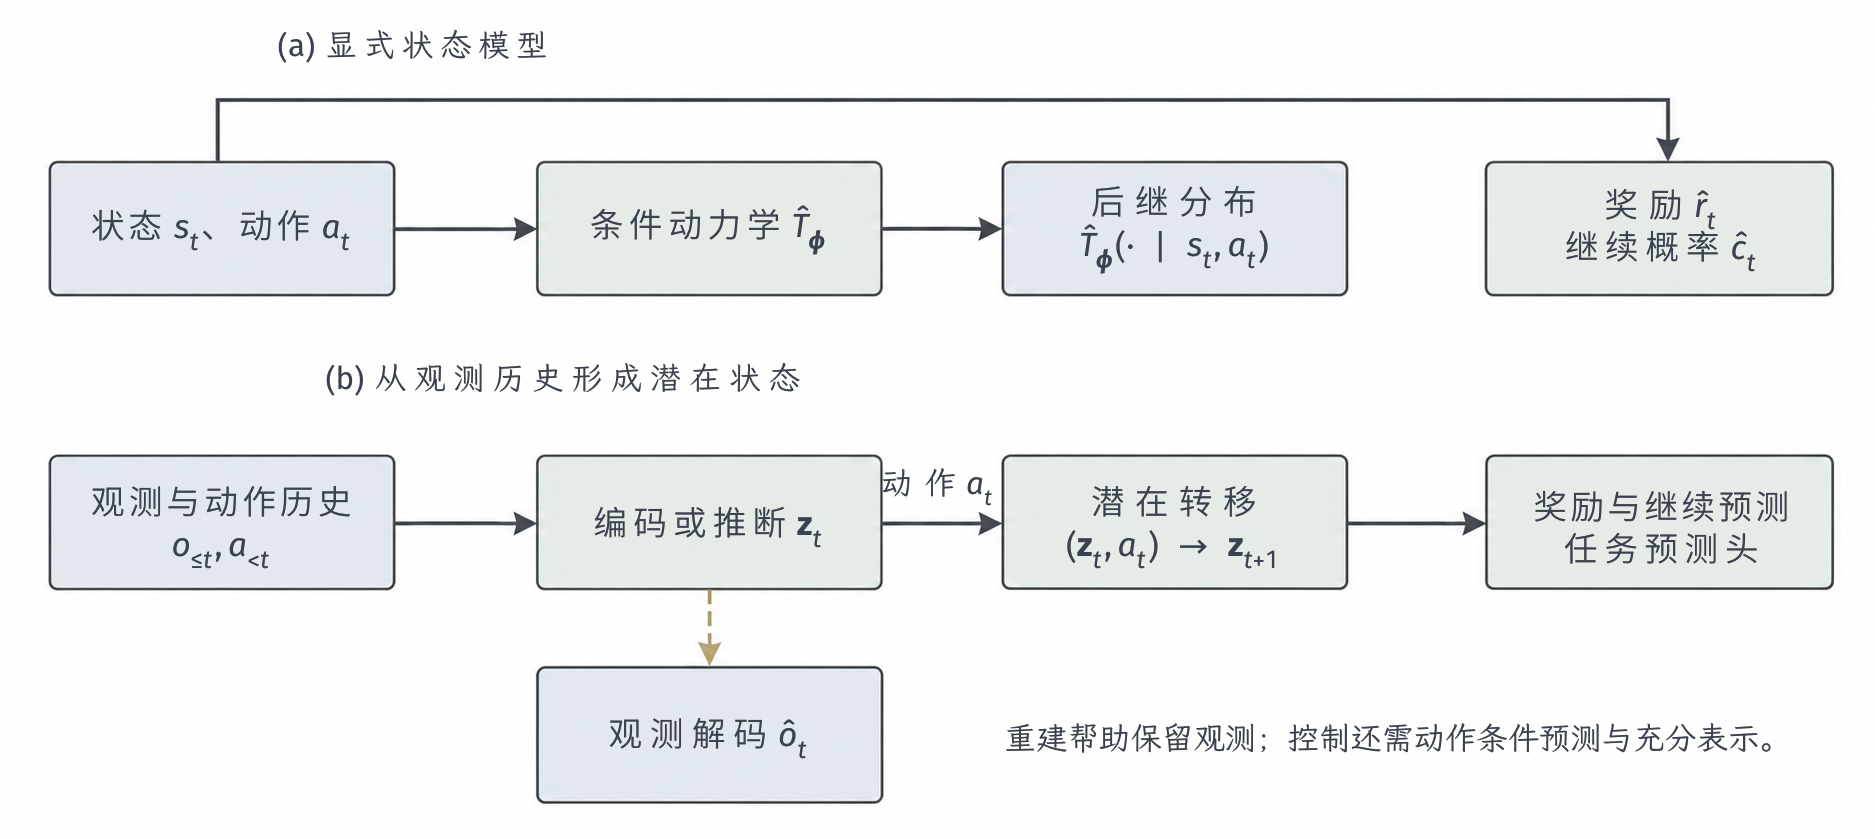
\includegraphics[width=157.400mm]{figures/10-reinforcement-learning/01-problems-and-solving/generated/rl-learning-model-anatomy/figure.png}
  \caption{学习模型的预测职责。上排直接预测可观测状态，下排先形成潜在状态；解码重建、奖励与继续预测是不同预测任务，是否需要每项预测取决于下游用途。虚线表示可选的重建支路，不表示模型生成经验。}
  \label{fig:rl-learning-model-anatomy}
\end{figure*}

\begin{table*}[t]
  \centering
  \small
  \begin{tabularx}{\linewidth}{>{\raggedright\arraybackslash}p{25mm} >{\raggedright\arraybackslash}X >{\raggedright\arraybackslash}X}
    \toprule
    表示与实例 & 拟合和保留什么 & 控制接口与局限 \\
    \midrule
    显式状态模型 & 对位置、速度等已定义状态拟合后继分布；奖励可已知或另学 & 可直接将后继送入价值函数；坐标误差须结合状态尺度与决策后果解释 \\
    World Models & 用VAE压缩图像，以混合密度递归模型预测潜在演化，控制器读取表示与记忆 & 控制器可用进化搜索训练；不同任务中模型承担表示或模拟器职责，不等于每步都做MPC \\
    PlaNet & 确定递归分量与随机潜变量共同形成RSSM；拟合观测、奖励及潜在多步关系 & 在潜在空间评估动作序列并执行首动作；搜索质量仍依赖模型滚动和状态推断 \\
    \bottomrule
  \end{tabularx}
  \caption{显式与潜在模型的区别。随机潜变量、参数后验和模型集成是不同层面的不确定性表示。}
  \label{tab:rl-learning-model-representations}
\end{table*}

\Needspace{18\baselineskip}
World Models展示了压缩视觉、递归预测与小型控制器的组合\scite{rl3-ha2018worldmodels}
PlaNet进一步将潜在模型直接用于在线规划，二者所需的训练目标与执行成本并不相同\scite{rl3-hafner2019planet}

评价模型时至少要分清三件事。一步测试误差检查测试转移样本所代表的状态动作分布上的局部预测；多步闭环误差检查策略根据预测状态继续行动后的偏离；不确定性校准检查标成某个置信水平的集合是否具有相应覆盖率。一个只在远离门口处略有坐标误差的模型，可能控制得很好；另一个平均误差更小的模型，若恰好把门前可通行格预测成墙另一侧，就会改变最优动作。在连续化房间示例中，两条预测只相差很小距离也可能落在碰撞边界两侧，后果不能按平均像素距离比较。

集成分歧可以定位模型之间尚未达成一致的区域，但所有成员若共享训练缺口、特征缺陷或错误归纳偏置，也可能一致地错。只有另有统计假设和校准过程时，集成方差才能解释为某种置信半径；不能把“多个网络很一致”直接换成“真实环境一定如此”。

% Outline: 3.4.2
\subsection{模型生成经验与价值更新}
\label{sec:rl-learning-dyna}

观察到通往终点的转移后，上游状态可能很久不再被访问，已取得的奖励样本却可以先通过已有模型影响上游估值。Dyna把真实经验更新和模型内规划接到同一Q-learning接口：先从真实样本学习，再抽取模型后果重复备份。对样本$(s,a,r,s',c)$，无论其来源如何，更新均为
\begin{equation}
  Q(s,a)\gets Q(s,a)+\alpha
  \left[r+\gamma c\max_bQ(s',b)-Q(s,a)\right].
  \label{eq:rl-learning-dyna-update}
\end{equation}
差别在于这条样本可能来自真实环境，也可能来自模型。图\ref{fig:rl-learning-dyna}用线型标出两类来源，算法\ref{alg:rl-learning-dyna}给出一个支持随机转移的表格版本。原始确定性Dyna-Q可以只记每个状态动作最后观察到的后果；随机网格应保存经验分布或学习一个能采样多种后果的模型\scite{rl3-sutton1991dyna}

\begin{figure*}[t]
  \centering
  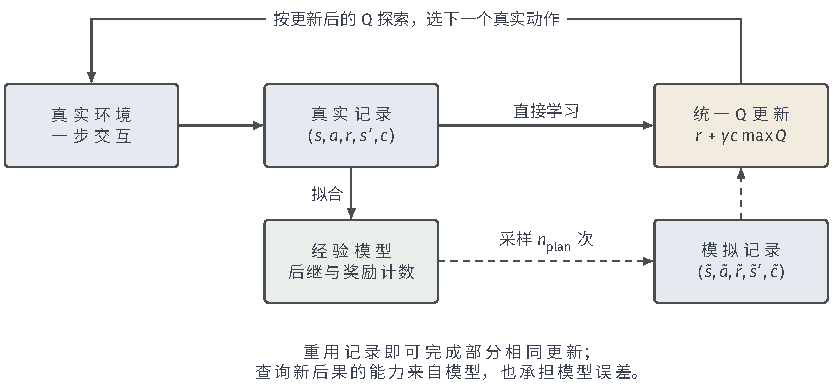
\includegraphics[width=140.959mm]{figures/10-reinforcement-learning/01-problems-and-solving/tikz/rl-learning-dyna.pdf}
  \caption{Dyna的转移记录生成与价值更新路径。实线为真实交互及其记录，虚线为学习模型生成的经验；两者进入同一种Q更新。模型采样次数是规划计算量，不是新增真实交互量。}
  \label{fig:rl-learning-dyna}
\end{figure*}

\begin{algorithm}[随机表格Dyna的一轮交互]
  \label{alg:rl-learning-dyna}
  \begin{algorithmic}[1]
    \State 在$s_t$按$Q$的探索策略选择$a_t$，真实执行并记录$(r_t,s_{t+1},c_t)$。
    \State 用式\eqref{eq:rl-learning-dyna-update}更新真实访问的$Q(s_t,a_t)$。
    \State 更新该状态动作的后继、奖励及继续标记计数，形成经验联合模型。
    \For{$i=1,\ldots,n_{\mathrm{plan}}$}
      \State 从已见状态动作中按指定规划分布选择$(\widetilde s,\widetilde a)$。
      \State 从当前经验模型采样$(\widetilde r,\widetilde s',\widetilde c)$。
      \State 用同一Q更新式更新$Q(\widetilde s,\widetilde a)$。
    \EndFor
    \State 若真正终止或达到环境的重置上限则重置；否则从$s_{t+1}$继续。仅时间截断时记录仍保留$c_t=1$及重置前的后继。
  \end{algorithmic}
\end{algorithm}

\begin{example}[不返回上游也能传播一次奖励]
  \label{ex:rl-learning-dyna-grid}
  在基准网格中，假设此前记录过
  $((3,2),\text{右},-0.04,(4,2),1)$，但当时所有Q值为0。
  现在从$(4,2)$向上恰好进入终点，用步长1把$Q((4,2),\text{上})$更新为1。
  若本轮模型从第一条记录生成相同转移，上游目标便为
  $-0.04+0.9\times1=0.86$。从当前上游Q值0出发、取规划步长$0.5$，一次模拟更新得到$0.43$，无需真实返回$(3,2)$。

  这是单条经验模型的一次更新，不是随机网格的精确Bellman备份。
  若其他后继的最大Q值仍为0，使用真实转移核的该次备份目标应为
  $-0.04+0.9(0.8\times1)=0.68$。模型中暂未记录的滑移不能因为多做模拟而消失。
\end{example}

对这条已经记录的转移，经验回放也能得到同样的$0.43$。模型的额外能力不在于重复这条算术，而在于按概率组合后果、查询未记录但可泛化到的动作，或递归生成新状态。表\ref{tab:rl-learning-generated-experience}因此把已有转移记录的复用与模型泛化分开。优先扫描还可按价值变化沿模型中的前驱关系分配规划次数；这种计算调度可以加快价值变化沿模型前驱关系的传播，但不能增加对未观察状态动作后果的真实验证。

\begin{table}[htbp]
  \centering
  \small
  \begin{tabularx}{\linewidth}{>{\raggedright\arraybackslash}p{21mm} >{\raggedright\arraybackslash}X >{\raggedright\arraybackslash}X}
    \toprule
    经验来源 & 可重用或生成什么 & 额外风险 \\
    \midrule
    经验回放 & 原始记录中的完整转移 & 覆盖不足、旧策略分布与相关性 \\
    经验表格模型 & 已见状态动作的估计后果，可求期望或采样 & 有限计数误差，重复模型采样不增加真实转移记录 \\
    参数化模型 & 在新的状态动作处预测，并递归滚动 & 分布外泛化、终止错误及虚构可达状态 \\
    \bottomrule
  \end{tabularx}
  \caption{真实记录与生成经验。更灵活的查询接口同时引入了更强的模型正确性要求。}
  \label{tab:rl-learning-generated-experience}
\end{table}

这也解释了优先扫描（prioritized sweeping）的调度对象。若某状态的价值刚大幅改变，模型中能一步到达它的状态动作称为它的前驱；优先备份这些前驱，再把新的变化向更早位置传播，就能把计算用在受影响的区域。这里的优先级控制模型备份顺序，与优先回放按记录残差改变抽样概率相关但不同；两者都不能替代一次新的真实试验。

Dyna增加多次分别采样的一步备份；也可以把连续几步预测合成当前状态的一次目标。这称为\term{模型价值扩展}（model-based value expansion, MVE）：短段奖励由模型预测，余下未来交给末端评论家。从真实回放状态$\widetilde s_0=s$出发，按待评价策略和学习模型滚动$L$步；令$\widetilde c_j$为继续标记，$w_0=1$、$w_{j+1}=w_j\widetilde c_j$，用累积继续权重屏蔽终止后的贡献，得到
\begin{equation}
  \widehat G^{\mathrm{MVE}}_0
  =\sum_{j=0}^{L-1}\gamma^j w_j\widetilde r_j
    +\gamma^L w_L V_{\bar{\bm w}}(\widetilde s_L).
  \label{eq:rl-learning-mve}
\end{equation}
奖励、后继和继续标记来自模型，起点来自真实回放中的状态记录，末端价值来自目标评论家。若预测的是联合期望，应对联合滚动取期望；不能在存在相关性时任意用各自边缘均值的乘积替代。以动作价值为目标时，第一步固定待更新动作，后续才由评价策略选动作。评论家把$\widehat G^{\mathrm{MVE}}_0$视为停止求导的目标，不在这一步沿模型反向优化策略\scite{rl3-feinberg2018mve}

若模型完全正确且没有终止，末端评论家的统一误差$\epsilon_V$只贡献$\gamma^L\epsilon_V$。增大$L$会衰减这项，却增加了需要正确预测的奖励和状态数。例如一个独立教学滚动有$L=2$、预测奖励$(0.1,0.2)$、末端价值$0.5$，则目标为$0.1+0.9(0.2)+0.9^2(0.5)=0.685$；若第二步错误预测为终止，就丢失$0.405$的末端贡献。滚动更长不是单向改善，也不能把生成一百万条轨迹解释为获得了一百万条独立真实证据。

% Outline: 3.4.3
\subsection{学习模型上的预测控制}
\label{sec:rl-learning-learned-mpc}

在当前状态，模型也可以直接比较候选计划，不必先将结果写进长期Q表。第\ref{sec:rl-planning-horizon-search}节的闭环仍然适用：优化计划，只执行首动作，再用新观测重新规划。新增条件是动力学由已采集的真实转移记录拟合；为控制计算量，每轮优化还限制为预先给定的开环动作序列。若不同随机后继需要不同后续动作，一条固定序列不能表示这种反馈选择，即使模型准确也有限制。因此，前章针对反馈决策树的前瞻保证不能直接移用。图\ref{fig:rl-learning-mpc}标明真实纠正发生在哪里：环境只反馈已执行动作，不会验证本轮所有候选轨迹。

\begin{figure*}[t]
  \centering
  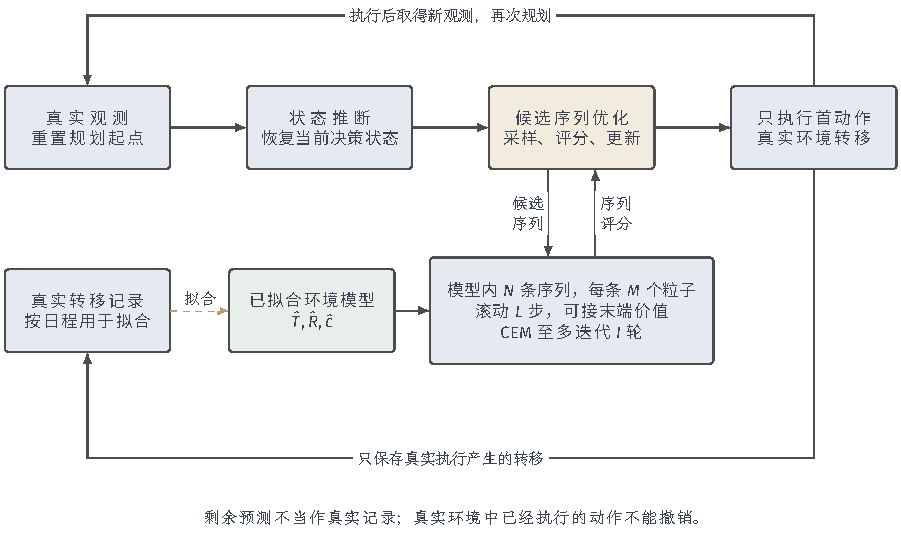
\includegraphics[width=152.615mm]{figures/10-reinforcement-learning/01-problems-and-solving/tikz/rl-learning-mpc.pdf}
  \caption{学习模型上的滚动规划。候选动作序列进入模型滚动，序列评分返回优化器；真实交互记录用于拟合环境模型。每轮从新观测建立规划起点，优化后只执行首动作；模型拟合可以较低频率进行，预测轨迹不会当作真实记录写回。}
  \label{fig:rl-learning-mpc}
\end{figure*}

当前规划的变量是一份动作序列，不是一份供所有状态调用的策略。在随机模型中，同一序列可能产生多条后继路径；粒子轨迹就是反复采样这些可能路径，用平均回报估计该序列的期望结果。候选数控制比较多少种计划，粒子数控制每种计划的评分波动，时域控制看多远。三者争用模型查询预算，增加一种数量不等于同时改善另外两种。

以有界连续动作$\bm u_j\in[\bm u_{\min},\bm u_{\max}]$为例，候选集合是长度$L$的合法动作序列。每条序列在模型中生成$M$个随机粒子轨迹，用平均预测奖励加末端价值估计期望回报，再选择评分较高的序列。评分为
\begin{equation}
  \widehat F(\bm u_{0:L-1};s)
  =\frac1M\sum_{m=1}^{M}
  \left[\sum_{j=0}^{L-1}\gamma^j\widehat r_j^{(m)}
          +\gamma^L\widehat V(\widehat s_L^{(m)})\right].
  \label{eq:rl-learning-particle-mpc}
\end{equation}
每个粒子从同一当前状态或其推断分布出发，经模型采样传播；终止时停止奖励并去掉末端价值。PETS（probabilistic ensembles with trajectory sampling，带轨迹采样的概率模型集成）使用概率动力学集成和轨迹粒子传播：模型内输出的噪声刻画随机后继，不同集成成员的预测差异反映模型拟合的不一致。其TS1传播可在每一步重选模型成员，TS$\infty$则让一个粒子在整个候选轨迹上保持同一成员；后者保留了“同一套动力学解释”在时间上的相关性，二者并不是同一个联合预测分布\scite{rl3-chua2018pets}

表\ref{tab:rl-learning-trajectory-optimizers}比较三种轨迹优化器。CEM在这里搜索的是本轮动作序列，不是前文跨状态共享的策略参数。一个可复现的教学配置为$L=5$、每轮$N=200$条候选、每条$M=20$个粒子、保留$E=20$条精英、最多$I=5$轮。初始化独立各维高斯，均值取上一步最优序列左移后的热启动，最后一步补零，标准差取动作范围的一半；第一轮没有历史序列时全取零均值。

\begin{table*}[t]
  \centering
  \small
  \begin{tabularx}{\linewidth}{>{\raggedright\arraybackslash}p{18mm} >{\raggedright\arraybackslash}X >{\raggedright\arraybackslash}X}
    \toprule
    优化器 & 候选和更新机制 & 奖励查询、梯度需求与预算 \\
    \midrule
    随机shooting & 从固定提议分布抽序列，选择预计回报最高者 & 无梯度；一次评估$N$条，不利用精英改变下一轮分布 \\
    CEM & 反复采样，截取精英，对序列分布重新做最大似然拟合 & 无梯度；需报告轮数、精英比例、方差下限及约束处理 \\
    MPPI & 对名义序列加入噪声，用指数回报或负成本权重平均扰动 & 标准路径积分推导有动力学与噪声匹配条件；通用采样实现需说明重要性校正与控制代价 \\
    \bottomrule
  \end{tabularx}
  \caption{同一模型目标的不同优化接口。PETS和PlaNet是模型与规划器的组合，不能与CEM这样的优化器放在互斥层级。}
  \label{tab:rl-learning-trajectory-optimizers}
\end{table*}

每轮从当前高斯采样并逐坐标裁剪到动作区间，按式\eqref{eq:rl-learning-particle-mpc}评分，取最高$E$条；并列按候选编号决定。用精英的逐坐标均值$\bm m_{\mathcal E}$和方差$\bm v_{\mathcal E}$更新
\[
  \bm m\gets\tfrac12\bm m+\tfrac12\bm m_{\mathcal E},
  \qquad
  \bm v\gets\max\{\bm v_{\min},
                      \tfrac12\bm v+\tfrac12\bm v_{\mathcal E}\},
\]
其中每个坐标的最小标准差预设为动作范围的$1\%$。此处“裁剪高斯”是具体实现选择，不冒充截断高斯的精确最大似然算法。完成5轮即停止，保留所有已评分候选中分数最高的一条，执行其首动作；不把未经重新评分的均值序列自动当成最佳候选。这样每个真实动作最多需要$INML=100\,000$次粒子转移调用，另加$INM$次末端价值调用。批量并行会改变耗时，但不改变这个查询计数。上述数字只用于明确预算，不是PETS的统一默认值。

MPPI式加权把本轮候选序列的评分$\widehat F_i$转成归一化权重，常写为$w_i\propto\exp((\widehat F_i-\max_j\widehat F_j)/\tau)$，其中$\tau>0$是温度，所有$w_i$的和为1。温度越小，相同评分差产生的权重比越悬殊；减去最大值只为数值稳定，不改变归一化权重。再用$\sum_iw_i\bm\epsilon_i$修正名义序列，其中$\bm\epsilon_i$是生成第$i$条候选时加入的序列扰动。如果采样分布不等于推导中的参考分布，或控制噪声结构改变，就须补相应权重，不能从这个指数形式单独推出路径积分最优控制结论\scite{rl3-williams2017mppi}

PlaNet把候选动作送入潜在动力学，以预测奖励评估序列，使用CEM选择动作；它不需要为每个候选解码整段像素。PETS则通常在给定状态坐标上预测动力学。两者都能闭环重规划，但预测对象、状态推断和每次查询成本不同。

墙边滑移说明重规划的边界。在基准网格的$(4,2)$向上，真实到达终点的概率是$0.8$，还可能左滑至$(3,2)$或撞右墙原地不动。一个错误模型若把成功概率估为$0.98$，短时域会高估立即结束的机会；过短时域且无末端价值又可能低估绕行，长时域则继续使用错误转移。下一次观测能告诉规划器这次是否滑移，却不能在动作执行前补回遗漏的风险。若把墙改成不可逆损失区域，重规划也无法撤销落入其中的动作；这种约束需要第\ref{chap:rl-trustworthy}章的安全条件，而不是单靠“闭环”一词。

% Outline: 3.4.4
\subsection{面向搜索的模型与表示}
\label{sec:rl-learning-muzero}

搜索比较向左和向右，直接需要的是各分支的奖励及长期价值，而非每个背景像素。若潜在模型在所用展开深度上保留这些预测量，并提供值得优先检查的动作，规划器就可能据此选择。MuZero学习的正是服务于搜索的表示、动力学和预测头，不要求潜在状态还原完整观测；免去重建并没有免去决策相关预测的准确性要求\scite{rl3-schrittwieser2020muzero}

MuZero的三个部件可沿一次决策理解。表示函数把当前真实历史变成搜索起点；动力学接收一个候选动作，输出预测奖励与潜在后继；预测头在该后继给出叶值及动作先验。先验只帮助分配搜索次数，搜索返回值还要沿边加上奖励，最后用访问统计形成动作分布。网络在这里同时帮助预测和安排搜索，最终决策仍包含搜索计算。

为避免与决策时可得历史$I_t$混淆，记表示函数为$e_{\bm\phi}$。从实际记录的可得历史编码得到$\bm z^0=e_{\bm\phi}(I_t)$，潜在动力学与预测头为
\begin{equation}
  (\widehat r^k,\bm z^{k+1})=g_{\bm\phi}(\bm z^k,a^k),
  \qquad
  (\bm p^k,\widehat v^k)=f_{\bm\phi}(\bm z^k).
  \label{eq:rl-learning-muzero-model}
\end{equation}
$\bm p^k$是动作先验，不是最终搜索访问分布；$\widehat v^k$是叶值，不是从根开始的全部回报。沿搜索边备份时仍需加边上奖励：
$G^k=\widehat r^k+\gamma G^{k+1}$。
如果一条新边预测奖励$-0.04$、后继叶值$0.8$，其返回值就是$0.68$，不能把$0.8$原样抄回父节点。

搜索还需要分配有限展开次数，既检查当前返回值高的动作，也检查先验看好但尚少访问的动作。已展开节点存储访问数$N(\bm z,a)$和平均返回值$\overline Q(\bm z,a)$。在合法分支上最大化“返回值加探索项”，可用常数探索系数的PUCT形式说明：
\[
  a\in\argmax_b\left[
    \overline Q(\bm z,b)
    +c\,p(b\mid\bm z)
      \frac{\sqrt{\sum_{b'}N(\bm z,b')}}{1+N(\bm z,b)}
  \right].
\]
实际MuZero还使用随访问数变化的系数、价值范围归一化和训练时根噪声等细节；应按任务实现保存配置。这一评分沿树选择到叶节点，调用一次潜在动力学生成新节点，查询预测头，再沿路径增加计数并更新均值。图\ref{fig:rl-learning-muzero}分开了搜索备份与训练监督。

\begin{figure*}[t]
  \centering
  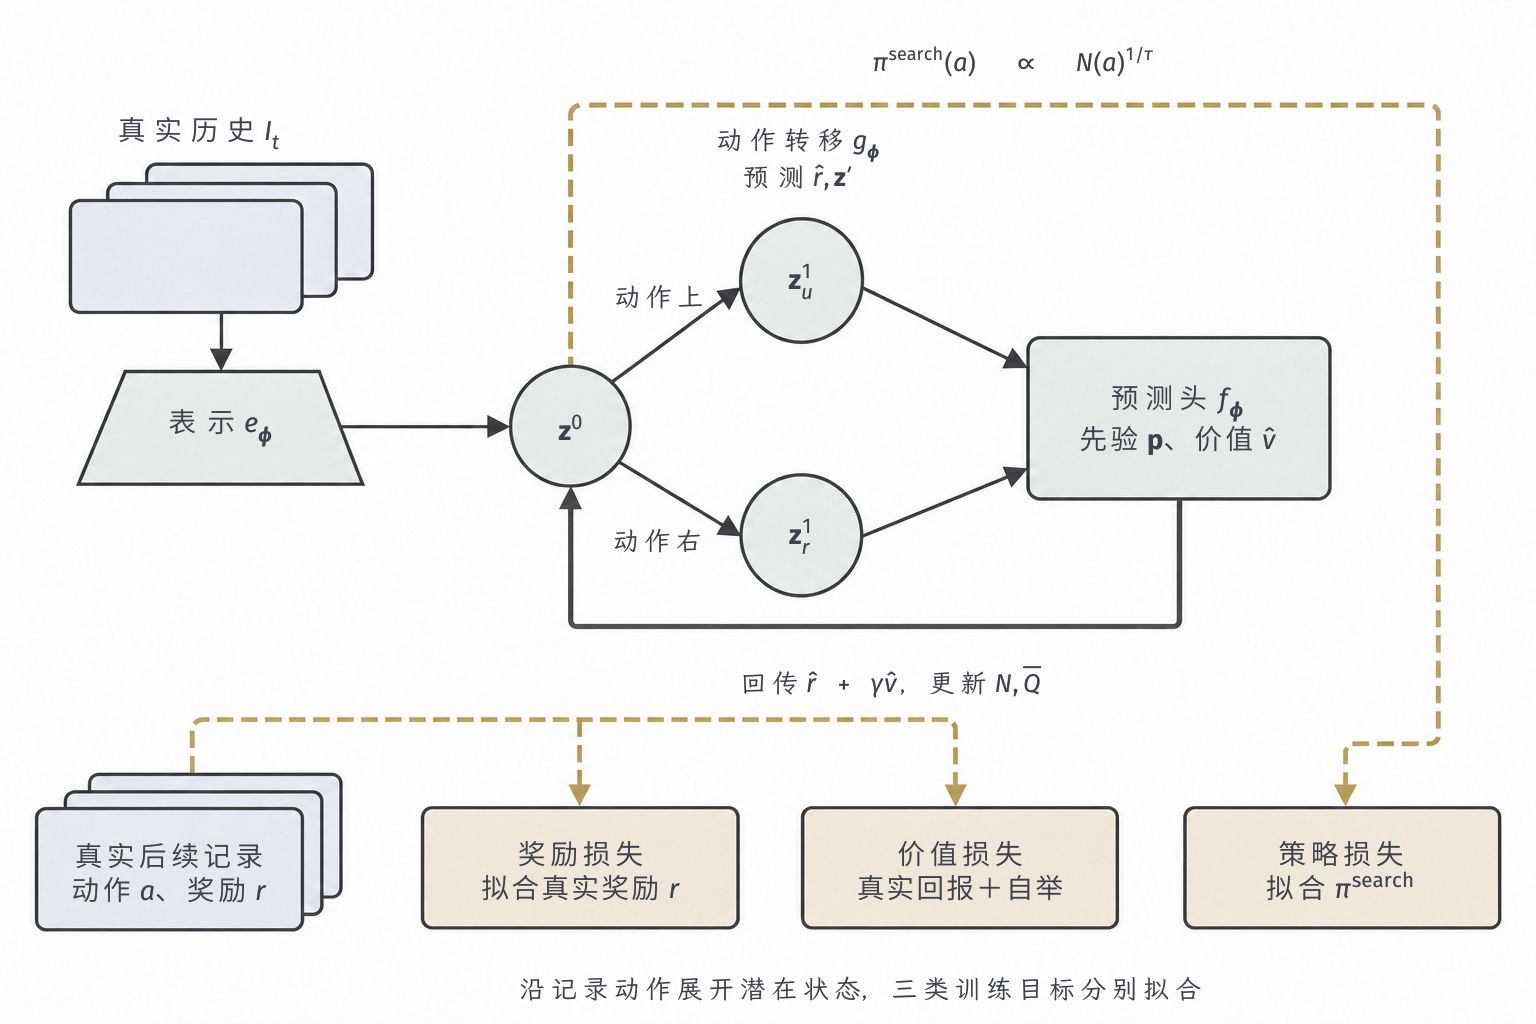
\includegraphics[width=157.400mm]{figures/10-reinforcement-learning/01-problems-and-solving/generated/rl-learning-muzero/figure.png}
  \caption{MuZero的搜索与学习。上部在潜在状态中展开并把边奖励加上折扣叶值传回根；下部用真实轨迹训练奖励与价值预测，用搜索访问分布训练策略先验。潜在后继不是新观测，访问分布也不是真实动作频率的简单重放。历史帧和搜索分支仅为示意，不固定历史长度或树规模。}
  \label{fig:rl-learning-muzero}
\end{figure*}

例如人工搜索快照中根节点先已有向右$N=2,\overline Q=0.85$，向上$N=1,\overline Q=0.6$；一次新展开给向右返回$0.68$，则其访问数变3、均值变$(2\times0.85+0.68)/3\approx0.7933$。若温度为1，四次访问对应策略目标$(3/4,1/4)$；温度趋于0时则集中到访问数最大的动作。这里的访问来自搜索模拟，不是环境在同一状态真实走了四步。

搜索得到的访问统计随后也用于训练网络。我们从真实回放取起点和后续动作，按记录动作展开$K$步：奖励头拟合真实奖励，价值头拟合真实奖励加末端搜索价值，策略头拟合搜索访问分布。令$\bm\pi^{\mathrm{search}}_{t+k}$为该时刻保存或重新计算的搜索策略目标，$z^V_{t+k}$为相应$n$步价值目标；下面的损失在各展开位置累加，按三类误差最小化模型参数：
\begin{align}
  z^V_t&=\sum_{j=0}^{n-1}\gamma^j r_{t+j}
                     +\gamma^n v^{\mathrm{search}}_{t+n}, \notag\\
  L_{\mathrm{MZ}}
    &=\sum_{k=0}^{K}
       \left[\ell_v(\widehat v^k,z^V_{t+k})
            -\sum_a\pi^{\mathrm{search}}_{t+k}(a)\log p^k_a\right]
      +\sum_{k=0}^{K-1}\ell_r(\widehat r^k,r_{t+k}).
  \label{eq:rl-learning-muzero-loss}
\end{align}
真实终止时截断奖励和自举；棋类可用最终胜负作为价值目标，Atari等还会使用变换后的离散价值表示。式中$r_{t+k}$仍是执行记录动作$a_{t+k}$后的奖励，不能把潜在展开的第一个奖励错位一格。优化损失更新三个模块；下一批真实交互再用新模块搜索，形成“搜索改进策略目标、网络拟合搜索结果”的循环。

训练中的策略目标来自搜索，价值与奖励目标又来自真实记录及末端估值。因此模型预测影响搜索，搜索影响下一批真实行为和训练目标，模型随后再拟合这些目标。搜索先验不是人工正确标签，而是这个反馈过程的一部分；模型在未验证的分支上出错时，搜索和学习也可能共同偏离真实任务。

EfficientZero针对有限真实交互训练样本补强这一循环：用记录后继的编码监督潜在展开的一致性，预测一段奖励的价值前缀以降低逐步奖励误差对备份的影响，并对旧策略轨迹记录的价值目标进行离策略修正和重新分析。以预测器$q$为例，一致性项可用
$-\operatorname{cos}(q(\widehat{\bm z}^{k}),\operatorname{sg}(e(o_{t+k})))$；
停止梯度使目标分支不被当前一致性损失同步更新，但它本身不能排除表示塌缩；实际稳定性还依赖完整训练设计。它是在MuZero搜索学习接口上提高已有交互记录的利用率，不是“增加一个重建头”就自动取得相同样本效率\scite{rl3-ye2021efficientzero}

表\ref{tab:rl-learning-model-requirements}将两种要求对照。一个模型在行为策略轨迹上准确预测价值，仍可能在很少训练过的动作组合和更深搜索中任意出错；因此“无需重建”免去的是一个输出要求，不是免去反事实检验。部署时MuZero仍主要依赖搜索访问统计选动作，单独取策略头最大值是另一个执行协议。

\begin{table*}[t]
  \centering
  \small
  \begin{tabularx}{\linewidth}{>{\raggedright\arraybackslash}p{26mm} >{\raggedright\arraybackslash}X >{\raggedright\arraybackslash}X}
    \toprule
    模型要求 & 直接训练或检查的对象 & 不能由此自动推出什么 \\
    \midrule
    可观测状态或图像重建 & 当前或未来可观测量的误差、似然 & 关键动作排序、未覆盖反事实及安全性 \\
    奖励、价值和策略预测 & 指定动作序列下的奖励、策略相关值及搜索分布 & 任意策略的回报、任意展开深度及完整环境规则 \\
    控制充分表示 & 在所需策略和干预集合上保留会影响动作选择的奖励或价值差别 & 超出这组策略、任务和干预后的继续有效性 \\
    \bottomrule
  \end{tabularx}
  \caption{重建与价值相关预测。要求应随模型实际承担的决策任务确定，不能按视觉精细程度排出统一优劣。}
  \label{tab:rl-learning-model-requirements}
\end{table*}

% Outline: 3.4.5
\subsection{潜在轨迹规划与价值引导}
\label{sec:rl-learning-tdmpc}

MuZero沿树分配离散分支的展开次数。连续动作下每个节点有无穷多候选，另一种接口是直接采样并优化短动作序列。TD-MPC将潜在动力学与TD价值结合：模型预测短段奖励和状态，末端评论家估计长尾回报，策略先验提出部分候选以缩小搜索范围。图\ref{fig:rl-learning-tdmpc}分开提议与执行，因为即使先验参与学习，最终动作仍由本轮规划评分决定。

\begin{figure*}[t]
  \centering
  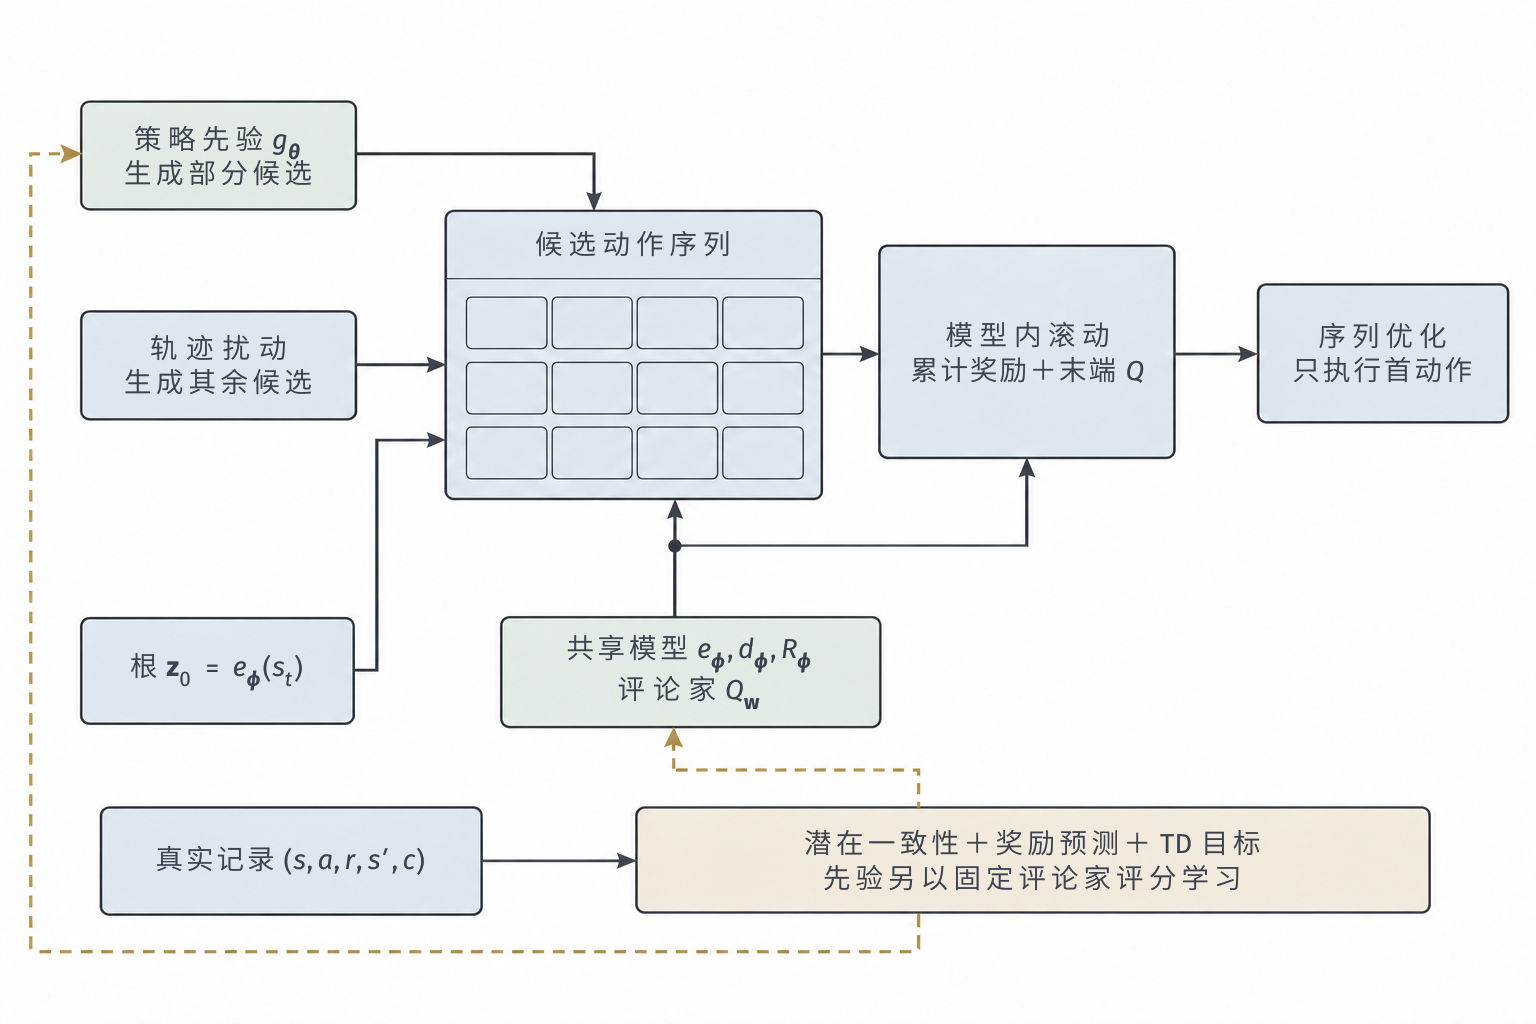
\includegraphics[width=157.400mm]{figures/10-reinforcement-learning/01-problems-and-solving/generated/rl-learning-tdmpc/figure.png}
  \caption{TD-MPC中的候选生成、模型评分与参数学习。各候选共享当前真实根；策略先验递归提出部分动作序列，其余候选由轨迹扰动形成。共享模型用于提议中的状态预测与候选评分，预测奖励累计后接末端Q；候选经回报加权或精英迭代优化后，只执行所求序列的首动作。训练虚线更新共享模型、评论家和先验参数，不指向某一条预测轨迹。轨迹格仅为示意，不规定候选数或规划时域。}
  \label{fig:rl-learning-tdmpc}
\end{figure*}

令策略先验的确定性动作映射为$g_{\bm\theta}$，其诱导策略为$\pi_{\bm\theta}(\mathrm da\mid\bm z)=\delta_{g_{\bm\theta}(\bm z)}(\mathrm da)$。先从当前真实状态编码$\bm z_0=e_{\bm\phi}(s)$，再按候选动作预测$\bm z_{j+1}=d_{\bm\phi}(\bm z_j,a_j)$。为了比较这些合法序列，评分累加前$L$步预测奖励，并在末端调用策略先验和评论家补上未展开部分：
\[
  \widehat F(a_{0:L-1})
  =\sum_{j=0}^{L-1}\gamma^j R_{\bm\phi}(\bm z_j,a_j)
      +\gamma^L Q_{\bm w}(\bm z_L,g_{\bm\theta}(\bm z_L)).
\]
上式先写规划片段内不终止的情形；有终止时，需像式\eqref{eq:rl-learning-mve}一样用继续标记屏蔽后续奖励和末端值。末端的$Q$已含末端动作的奖励，前面的和只到$L-1$，从而没有重复计数。候选可以混合高斯扰动序列与策略先验滚动；按回报加权或选精英迭代优化后，只执行首动作。即使先验在训练中不断提高，最终动作也未必等于$g_{\bm\theta}(\bm z_0)$。

真实短序列支持三类损失。用$\operatorname{sg}$表示停止梯度，以单步标量形式说明其关系：
\begin{align}
  y_t&=r_t+\gamma c_t
      Q_{\bar{\bm w}}(\bar{\bm z}_{t+1},
                             g_{\bm\theta}(\bar{\bm z}_{t+1})), \notag\\
  \ell_t&=\lambda_z\|
        d_{\bm\phi}(\bm z_t,a_t)-\operatorname{sg}(\bar{\bm z}_{t+1})
                              \|_2^2
       +\lambda_r(R_{\bm\phi}(\bm z_t,a_t)-r_t)^2 \notag\\
       &\quad+\lambda_Q(Q_{\bm w}(\bm z_t,a_t)
                                      -\operatorname{sg}(y_t))^2.
  \label{eq:rl-learning-tdmpc-loss}
\end{align}
\Needspace{14\baselineskip}
$\bar{\bm z}_{t+1}$由目标编码器对真实后继编码；多步训练时，预测分支沿记录动作递归展开，并按深度加权这些损失\scite{rl3-hansen2022tdmpc}
策略先验通过提高$Q(\bm z,g_{\bm\theta}(\bm z))$学习，优化它时需固定评论家参数；模型和价值训练则使用记录动作。目标网络、归一化、正则化及实际Q集合依具体版本而定，式\eqref{eq:rl-learning-tdmpc-loss}展示原始方法的核心接口，不是TD-MPC2全部实现细节。

TD-MPC2继续使用短潜在规划和末端价值，但对潜在状态做SimNorm归一化，采用离散分布式奖励与价值预测、Q集成和最大熵策略先验等设计来增强跨任务训练稳定性。若把向量分成多个小组，每组softmax后的分量非负且和为1，SimNorm便限制了潜在表示的尺度；这不等于获得了动力学误差的统计置信界。分布式目标改善不同奖励尺度的优化，Q集成抑制部分过估计，也不能替代真实访问覆盖。

TD-MPC2原论文报告104个在线任务、四类任务域，并另有多任务规模实验；其中317M参数、80任务的设置不能当成所有对比方法统一使用的预算。其结果支持的是相应交互训练记录、模型和任务协议下的经验结论，不是“潜在规划必然优于树搜索”的一般排序\scite{rl1-hansen2024-tdmpc2}

表\ref{tab:rl-learning-planning-budgets}按模型查询而不是名称比较三种接口。在固定总查询数$B$下，$N$条长度$L$、每条$M$粒子的轨迹大致消耗$NLM$次转移查询；树搜索可能每次模拟只扩展一个新节点，但还需遍历已建路径和维护统计。神经网络批处理、动作维数和叶值计算成本都不同，查询数相同仍不等于墙钟时间相同。

\begin{table*}[t]
  \centering
  \small
  \begin{tabularx}{\linewidth}{>{\raggedright\arraybackslash}p{23mm} >{\raggedright\arraybackslash}X >{\raggedright\arraybackslash}X >{\raggedright\arraybackslash}X}
    \toprule
    规划接口 & 主要查询模块 & 动作结构 & 预算分配 \\
    \midrule
    潜在树搜索 & 表示、动力学、奖励、策略先验、叶值 & 有限分支最直接；连续动作需额外候选机制 & 在重复访问的分支间分配展开，并复用树中统计 \\
    轨迹采样 & 动力学、奖励，可选末端价值 & 向量动作及显式约束便于联合采样 & 候选数、粒子数、时域和迭代轮数相互争用预算 \\
    价值引导短规划 & 潜在动力学、奖励、末端Q、策略先验 & 常用于连续控制 & 用评论家替代长尾滚动，把查询用于短轨迹优化 \\
    \bottomrule
  \end{tabularx}
  \caption{相同模型查询预算下仍需区分的计算。价值引导是轨迹评估的组成方式，可以与不同采样优化器组合。}
  \label{tab:rl-learning-planning-budgets}
\end{table*}

% Outline: 3.4.6
\subsection{模型偏差与规划边界}
\label{sec:rl-learning-model-bias}

验证集上的低平均误差未必保护规划动作，因为规划器查询模型的方式不是随机平均：它专门寻找预计回报最高的候选。当某个少覆盖分支被高估，增加搜索反而可能更稳定地找到它。这称为\term{模型利用偏差}（model exploitation），即优化器将预测错误当成可利用收益。图\ref{fig:rl-learning-model-exploitation}与下面的两路线例子展示了这一选择过程。

\begin{example}[优化器选择了最乐观的错误]
  \label{ex:rl-learning-model-exploitation}
  将网格局部改成两个可选路线的独立教学任务。安全路线的真实与预测回报都为$0.6$；稀少访问的“捷径”进入终点的真实概率为$0.1$，失败进入零回报吸收态，即真实回报$0.1$。模型却把成功概率估为$0.9$，于是预计回报$0.9$并反复选择捷径。
  若测试转移样本所代表的路线分布有$99\%$质量落在安全路线，则按该分布计算的平均绝对回报误差仅为$0.01\times0.8=0.008$，实际选择的动作却损失$0.5$。
  增加规划候选数可以更稳定地选中这个错误最大值，并不会自动降低误差。
\end{example}

\begin{figure}[htbp]
  \centering
  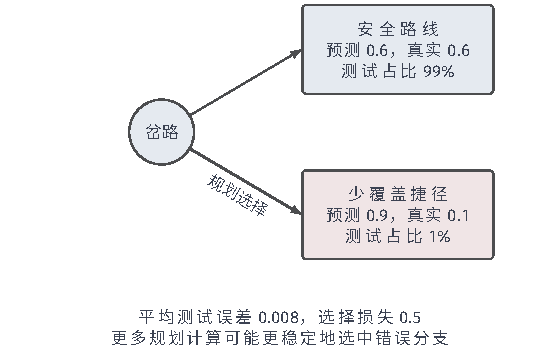
\includegraphics[width=94.749mm]{figures/10-reinforcement-learning/01-problems-and-solving/tikz/rl-learning-model-exploitation.pdf}
  \caption{少覆盖分支上的模型利用偏差。数字属于例\ref{ex:rl-learning-model-exploitation}的人工两路线任务；模型内最优动作与真实最优动作相反，测试分布的低平均误差掩盖了这一差别。}
  \label{fig:rl-learning-model-exploitation}
\end{figure}

要把模型误差变成价值误差，需要说明误差在哪些状态动作上受控。下面给出一个统一但较强的条件；它不需要模型来自某种特定学习算法，也不会从经验损失小自动成立。

\begin{theorem}[固定策略的模型误差界]
  \label{thm:rl-learning-simulation}
  在相同有限状态动作空间、折扣$0\leq\gamma<1$上，两个MDP的奖励均值为$R,\widehat R$、转移核为$T,\widehat T$。假设两者奖励均值绝对值均不超过$R_{\max}$，并且对每个合法$(s,a)$，
  \[
    |R(s,a)-\widehat R(s,a)|\leq\varepsilon_R,\qquad
    \sum_{s'}|T(s'\mid s,a)-\widehat T(s'\mid s,a)|
       \leq\varepsilon_T.
  \]
  对任意固定平稳策略$\pi$，记两个模型中的价值为$V^\pi,\widehat V^\pi$，则
  \begin{equation}
    \|V^\pi-\widehat V^\pi\|_\infty
       \leq B_{\mathrm{model}}
       :=\frac{\varepsilon_R}{1-\gamma}
        +\frac{\gamma R_{\max}\varepsilon_T}{(1-\gamma)^2}.
    \label{eq:rl-learning-simulation-bound}
  \end{equation}
  在相同初始分布下，$|J(\pi)-\widehat J(\pi)|$也不超过$B_{\mathrm{model}}$。
\end{theorem}

\begin{proof}
  对策略动作取平均后，奖励误差仍不超过$\varepsilon_R$，每一行转移分布的$L^1$误差仍不超过$\varepsilon_T$。由奖励界，
  $\|\widehat V^\pi\|_\infty\leq R_{\max}/(1-\gamma)$。
  相减两个Bellman方程，并加减$\gamma T^\pi\widehat V^\pi$，得到
  \[
    V^\pi-\widehat V^\pi
     =R^\pi-\widehat R^\pi
       +\gamma T^\pi(V^\pi-\widehat V^\pi)
       +\gamma(T^\pi-\widehat T^\pi)\widehat V^\pi .
  \]
  因$T^\pi$是随机矩阵，其中间项的无穷范数至多为
  $\gamma\|V^\pi-\widehat V^\pi\|_\infty$。对末项逐行用三角不等式，
  \[
    \|(T^\pi-\widehat T^\pi)\widehat V^\pi\|_\infty
      \leq\varepsilon_T\|\widehat V^\pi\|_\infty
      \leq\frac{R_{\max}\varepsilon_T}{1-\gamma}.
  \]
  合并三项并把带$\gamma$的价值差移到左边，即得式\eqref{eq:rl-learning-simulation-bound}。最后对相同$\mu_0$取期望，概率加权平均不超过无穷范数，得到回报差结论。
\end{proof}

这种论证通常称为模拟引理的一个形式。这里$\varepsilon_T$是$L^1$误差；若用总变差$\operatorname{TV}=\tfrac12\|\cdot\|_1$定义误差，转移项系数必须相应改变，不能直接抄同一个常数。原始有限MDP学习分析中的模拟论证也是把局部模型误差传到长期回报，但具体时域与误差规范应按所引用结果区分\scite{rl3-kearns2002efficient}

固定策略误差界还能支持模型内选出的策略，但需要误差条件统一覆盖候选所需的全部状态动作。设规划在学习模型的合法策略中最大化$\widehat J$，输出$\widehat\pi$的次优度至多$\epsilon_{\mathrm{plan}}$。若上述统一误差事件成立，模型界就同时适用于真实最优策略和依据模型训练记录选出的$\widehat\pi$。将真实性能差拆成两侧模型误差和中间规划误差，得到
\begin{align*}
  J(\pi^*)-J(\widehat\pi)
   &=J(\pi^*)-\widehat J(\pi^*)
     +\widehat J(\pi^*)-\widehat J(\widehat\pi)
     +\widehat J(\widehat\pi)-J(\widehat\pi)\\
   &\leq 2B_{\mathrm{model}}+\epsilon_{\mathrm{plan}}.
\end{align*}
中间项利用了$\widehat J(\pi^*)\leq\max_\pi\widehat J(\pi)$。若仅知道某个固定行为策略的模型误差小，第一和第三项不能同时这样控制，尤其不能把训练之后挑出的策略当成预先固定的策略。

表\ref{tab:rl-learning-model-validity}归纳了检验层次。更精细的分析可以按占用分布加权误差，减少统一界的保守性，但要补上策略覆盖或分布转移的控制。重建误差、模型似然和集成分歧都可能是有用诊断量；它们各自需要通往决策目标的论证。基于模型置信集合的鲁棒优化与风险约束留到第\ref{chap:rl-trustworthy}章。

\begin{table*}[t]
  \centering
  \small
  \begin{tabularx}{\linewidth}{>{\raggedright\arraybackslash}p{24mm} >{\raggedright\arraybackslash}X >{\raggedright\arraybackslash}X}
    \toprule
    检验层次 & 它回答的问题 & 仍需补充的条件 \\
    \midrule
    重建质量 & 已观察内容能否编码并还原 & 决策相关量是否保留、历史是否充分 \\
    预测一致性 & 已覆盖动作序列的预测是否吻合 & 更长滚动、策略变化及误差校准 \\
    反事实正确性 & 换动作后模型是否仍有效 & 对所需干预的真实覆盖或可识别结构 \\
    控制充分性 & 用该表示和模型是否保持所需策略的决策质量 & 具体任务、策略类、规划深度与误差到性能的联系 \\
    \bottomrule
  \end{tabularx}
  \caption{模型质量不是一个无条件通用的分数。前一行通过并不自动保证后一行通过。}
  \label{tab:rl-learning-model-validity}
\end{table*}

% Outline: 3.5
\section{基于模型的策略优化}
\label{sec:rl-learning-model-policy}

当前规划只为这次状态求一个动作或动作序列，下次仍需重新搜索。若要训练一份可以跨状态重复调用的策略，优化变量就从本轮$a_{0:L-1}$改成共享参数$\bm\theta$。模型可以让回报梯度经过预测动力学传到策略，也可以生成经验供行动者—评论家训练。两者都将大量计算放在训练阶段，部署动作主要来自训练后的策略；但策略读取的状态仍可能需要模型依据新观测推断。

% Outline: 3.5.1
\subsection{模型梯度与策略搜索}
\label{sec:rl-learning-model-gradient}

先考察模型如何提供真实环境无法直接给出的导数。在连续控制中，策略改变本步动作，动作改变后继状态，后继又改变下一次策略输出；求导需要保留整条依赖。先用一个只有两步的系统观察这些路径，再写一般递推。

\begin{example}[两步模型梯度]
  \label{ex:rl-learning-two-step-gradient}
  将连续控制简化为无噪声标量系统$x_{t+1}=ax_t+bu_t$，$u_t=\theta x_t$，固定$x_0=1$，仅有末端成本$C=x_2^2/2$。记$q=a+b\theta$，则$x_1=q$、$x_2=q^2$，所以
  \[
    \frac{\partial x_1}{\partial\theta}=b,\qquad
    \frac{\partial x_2}{\partial\theta}
       =q b+b x_1=2bq,\qquad
    \frac{\partial C}{\partial\theta}=2bq^3.
  \]
  人工取$a=b=1,\theta=-0.5$，梯度为$0.25$；学习率$0.1$的一次成本下降更新给$\theta'=-0.525$。若在第二步把输入状态$x_1$整体停止求导，便会丢掉上式的$q b$项，只留下本步参数直接改变动作的$b x_1$项，成本梯度变为$0.125$，恰好少一半。仅漏掉第二次策略调用中的状态导数并不等于这个操作，因为动力学对$x_1$的直接依赖仍可传回梯度。
\end{example}

设学到的动力学可重参数化为
$\bm x_{t+1}=f_{\bm\phi}(\bm x_t,\bm u_t,\bm\xi_t)$，策略为
$\bm u_t=g_{\bm\theta}(\bm x_t)$，$\bm\xi_t$是分布与策略参数无关的随机噪声。这里$g_{\bm\theta}$是确定性动作映射，其诱导策略是$\pi_{\bm\theta}(\mathrm du\mid\bm x)=\delta_{g_{\bm\theta}(\bm x)}(\mathrm du)$。固定模型参数$\bm\phi$并对一条采样轨迹求导，记
$\bm D_t=\partial\bm x_t/\partial\bm\theta$。由链式法则，
\begin{equation}
  \bm D_{t+1}
   =\left(f_{\bm x}+f_{\bm u}g_{\bm x}\right)\bm D_t
       +f_{\bm u}g_{\bm\theta},\qquad \bm D_0=\bm0.
  \label{eq:rl-learning-model-chain}
\end{equation}
这里$f_{\bm x},f_{\bm u}$分别是动力学对状态、动作的Jacobian，$g_{\bm x},g_{\bm\theta}$分别是策略对状态、参数的Jacobian，均在当前滚动状态、动作和噪声上计算。第二项是本步参数直接改变动作的影响，第一项保留先前动作经状态传来的影响。把这些敏感度乘上成本导数，就能得到模型内策略的下降方向。若有限时域成本为
$C(\bm\theta)=\mathbb E\sum_{t=0}^{L-1}c(\bm x_t,\bm u_t)+
\mathbb E c_L(\bm x_L)$，则
\[
 \nabla_{\bm\theta}C
  =\mathbb E\left[
    \sum_{t=0}^{L-1}
      \left(\bm D_t^\top\nabla_{\bm x}c_t+
       (g_{\bm x}\bm D_t+g_{\bm\theta})^\top
                                       \nabla_{\bm u}c_t\right)
          +\bm D_L^\top\nabla c_L(\bm x_L)\right].
\]
这里成本越小越好，与本章奖励最大化的关系是$r_t=-c_t$。将导数移入期望需要可微性和可积控制；接触、碰撞、离散动作及硬终止并不会自动满足这些条件。图\ref{fig:rl-learning-model-gradient}区分了训练模型与借模型训练策略的两条路径。

\begin{figure*}[t]
  \centering
  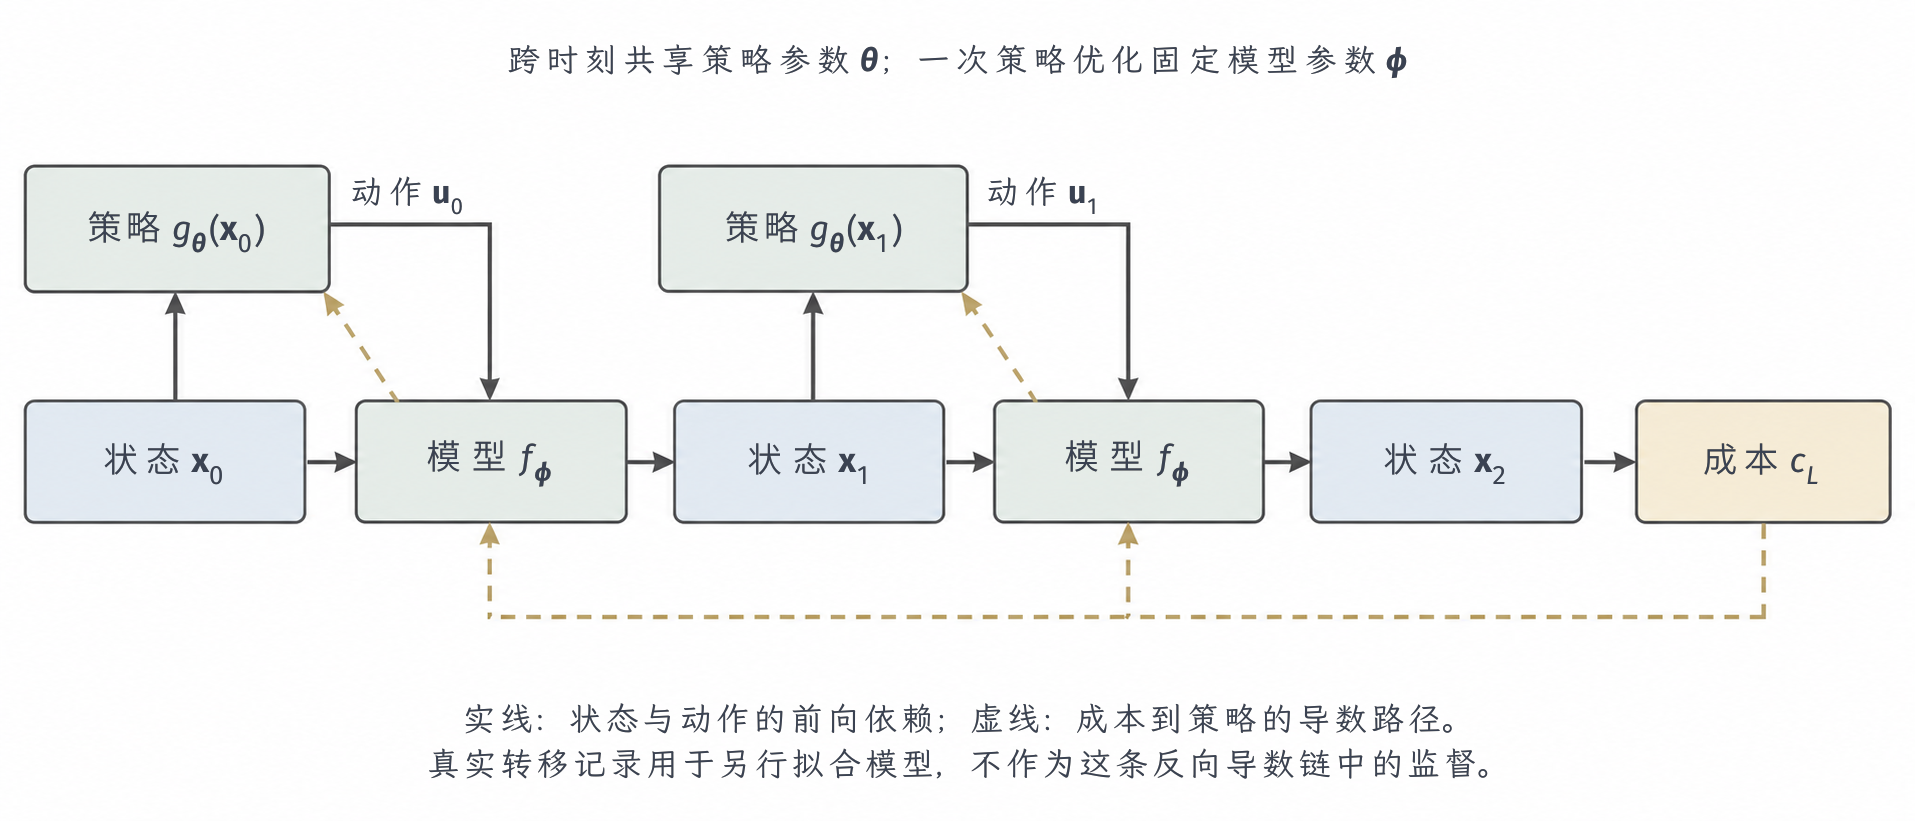
\includegraphics[width=157.400mm]{figures/10-reinforcement-learning/01-problems-and-solving/generated/rl-learning-model-gradient/figure.png}
  \caption{模型中的策略展开。每个时刻调用同一组策略参数，后继状态又进入策略；实线为前向依赖，虚线为策略优化时的反向导数。模型参数由真实转移训练记录更新，在一次策略梯度计算中固定，不因允许梯度穿过模型就同时最小化模型预测损失。}
  \label{fig:rl-learning-model-gradient}
\end{figure*}

一般递推正好包含刚才两步例中的两种影响。$\bm D_t$保存此前参数变化已经造成的状态变化；本步又通过$g_{\bm\theta}$直接改变动作。旧状态变化一方面通过动力学的$f_{\bm x}$传向后继，另一方面先改变本步策略输出，再通过$f_{\bm u}g_{\bm x}$传向后继。把这两条旧影响与本步新影响相加，才不会漏掉后续策略对输入状态的依赖。

采样路径求导需要处理随机轨迹；另一种方式是直接传播状态分布的近似参数。PILCO使用高斯过程描述动力学增量，同时保留给定动力学训练记录后的均值预测和不确定性。给定近似高斯的状态分布与参数策略，它通过矩匹配，让近似分布的均值和协方差等于所算的后继矩，递推状态分布，再对期望长期成本求导。把分布参数合记为
$\bm m_t=(\bm\mu_t,\operatorname{vec}\bm\Sigma_t)$，递推写成
$\bm m_{t+1}=F_{\bm\phi}(\bm m_t,\bm\theta)$，则
\[
 \frac{\partial\bm m_{t+1}}{\partial\bm\theta}
  =\frac{\partial F_{\bm\phi}}{\partial\bm m_t}
       \frac{\partial\bm m_t}{\partial\bm\theta}
       +\frac{\partial F_{\bm\phi}}{\partial\bm\theta}.
\]
期望成本$\bar c(\bm m_t)$的导数再乘这些敏感度。高斯近似使计算可行，却可能丢失多峰分布；高斯过程后验不确定性也依赖核和噪声假设。这个过程不是对真实非线性轨迹分布的精确积分\scite{rl3-deisenroth2011pilco}

模型也可作为黑盒评分器。固定$\bm\theta$，用它在模型里产生完整行为，再以采样回报驱动第\ref{sec:rl-learning-regularized-search}节的搜索；这不要求动力学可微，但需要更多候选评估。表\ref{tab:rl-learning-model-gradient-interfaces}对比所需的奖励查询、模型导数与随机变量密度。

\begin{table*}[t]
  \centering
  \small
  \begin{tabularx}{\linewidth}{>{\raggedright\arraybackslash}p{25mm} >{\raggedright\arraybackslash}X >{\raggedright\arraybackslash}X}
    \toprule
    接口 & 需要模型提供什么 & 主要计算与误差来源 \\
    \midrule
    采样路径反向传播 & 可微转移、奖励和策略；噪声可重参数化或另作梯度估计 & 保存或重算长度$L$的展开，导数连乘可能消失或爆炸；采样方差与模型导数偏差 \\
    分布传播的解析近似 & 可计算的分布矩、期望成本及其导数 & 传播均值和协方差；对分布形状、核和成本形式有要求，矩近似引入偏差 \\
    黑盒策略搜索 & 候选参数对应的模型回报样本 & 多候选、多噪声重复评分；不需模型Jacobian，仍会利用错误的回报排序 \\
    \bottomrule
  \end{tabularx}
  \caption{模型参与策略搜索的三种方式。可微性减少了部分搜索成本，但给模型增加了导数质量要求。}
  \label{tab:rl-learning-model-gradient-interfaces}
\end{table*}

预测误差小和导数准确是两件事。例如真实一步模型$f(u)=u$，近似模型
$\widehat f(u)=u+\epsilon\sin(\omega u)$，全域预测误差不超过$\epsilon$，而导数误差为$\epsilon\omega\cos(\omega u)$，可随$\omega$任意增大。在$u=0$两者输出甚至完全相同。前节的价值误差界控制函数值，不控制这个导数；借模型求梯度还应检查策略会用到的局部敏感度，或用真实交互的回报记录检验更新是否确实改进。

% Outline: 3.5.2
\subsection{想象轨迹中的行动者—评论家}
\label{sec:rl-learning-dreamer}

模型不必只提供导数，也可以在昂贵真实交互之间反复产生策略训练轨迹。World Models将观测编码为潜在变量，用循环模型预测后继，并在模型内搜索控制器参数。Dreamer则将这个训练环境接到行动者—评论家：策略在模型中行动，评论家评价预测回报，行动者再根据评价改进。这样复用的是学习到的预测规律，而不是新增真实证据\scite{rl3-ha2018worldmodels}

模型内训练可先按三个阶段理解。真实轨迹提供观测、动作和结果，用来训练模型；从其中一个已有观测历史推断当前内部状态，再让固定模型模拟若干步，形成策略训练材料；最后把策略拿回真实环境测试。模拟中看见的是模型预测，只有重新执行真实动作才会增加环境证据。“想象”指这段不再读取未来真实观测的模拟，不指随意编造与动作无关的画面。

\begin{definition}[想象轨迹]
  \label{def:rl-learning-imagination}
  给定一段真实观测与动作历史，先按模型的潜在后验抽取起点，再由固定的潜在转移模型和策略逐步生成后继潜变量与动作，并由预测头给出奖励和继续概率。这个模型内序列称为想象轨迹。后验属于拟合的潜在模型，不是未经证明就等于真实环境隐状态的条件分布；离开起点后没有新观测时，后继按模型先验生成，不能读取未来真实观测的编码。
\end{definition}

要区分真实起点与想象后继，需要明确模型在有观测和无观测时怎样更新。循环状态空间模型（RSSM）用确定性记忆保存历史递推，用随机潜变量表示当前状态的条件不确定性。为避免与真实历史$I_t$混用，分别记为$\bm m_t,\bm z_t$，合状态为$\bm x_t=(\bm m_t,\bm z_t)$。真实序列用观测更新后验；想象时没有新观测，只能从先验预测前进。仍把执行动作$a_t$后得到的奖励记为$r_t$：
\begin{align}
 \bm m_{t+1}&=f_{\bm\phi}(\bm m_t,\bm z_t,a_t),\notag\\
 q_{\bm\phi}(\bm z_{t+1}\mid\bm m_{t+1},o_{t+1})
       &\quad\text{用于真实观测序列的后验推断},\notag\\
 p_{\bm\phi}(\bm z_{t+1}\mid\bm m_{t+1})
       &\quad\text{用于无后续观测的先验滚动}.
 \label{eq:rl-learning-rssm}
\end{align}
奖励$r_t$及是否继续$c_t$的预测可在该转移的后继潜在状态上读出。若实现把进入状态时的奖励记作$r_{t+1}$，只须整体对齐索引，不能把旧观测之后、动作之前的奖励混进同一个目标。

这里的先验与后验比较的是同一个潜在状态。动作后、尚未看到$o_{t+1}$时，$p_{\bm\phi}$依据已有记忆预测它；看到新观测后，$q_{\bm\phi}$再用观测修正判断。真实序列能学习这种修正，无观测的想象序列只能使用预测。模型训练需要让预测接近带观测的修正，才可能从真实起点继续滚动；两者都是学习模型中的分布，不能直接认作真实隐藏状态分布。

真实序列中的观测、奖励和继续变量提供预测监督，但只有这三项还不足以训练无观测滚动：模型还需使先验接近带观测的后验。以DreamerV3的离散潜变量为例，记$q_t,p_t$为同一时刻的后验、先验。下面先累加三类负对数似然，再用分别停止一侧梯度的KL项训练先验和表示；模型参数最小化其真实序列期望：
\begin{align}
 \ell_{\mathrm{pred},t}
   &=-\log p_{\bm\phi}(o_t\mid\bm x_t)
     -\log p_{\bm\phi}(r_{t-1}\mid\bm x_t)
     -\log p_{\bm\phi}(c_{t-1}\mid\bm x_t),\notag\\
 \ell_{\mathrm{dyn},t}
   &=\max\{1,D_{\mathrm{KL}}(\operatorname{sg}(q_t)\|p_t)\},\notag\\
 \ell_{\mathrm{rep},t}
   &=\max\{1,D_{\mathrm{KL}}(q_t\|\operatorname{sg}(p_t))\},\notag\\
 L_{\mathrm{model}}&=\mathbb E\sum_t
       [\ell_{\mathrm{pred},t}+\ell_{\mathrm{dyn},t}
                         +0.1\ell_{\mathrm{rep},t}].
 \label{eq:rl-learning-dreamer-model}
\end{align}
序列首项没有对应转移监督时省去奖励和继续损失。这里$r_{t-1}$明确指进入$\bm x_t$的上一步奖励，并未改动本章的经验定义。两项KL分别调整先验和表示。nat是采用自然对数时熵与KL散度的计量单位，$1$ nat等于$1/\log2$ bit；这里的阈值1按该尺度计量散度。KL低于1 nat时，上述最大值取常数1，不再施加这项KL梯度压力；实际离散分布还混入$1\%$均匀概率以避免极端概率。观测重建帮助训练表示，但不能单独证明其对所有控制干预充分。

\begin{figure*}[t]
  \centering
  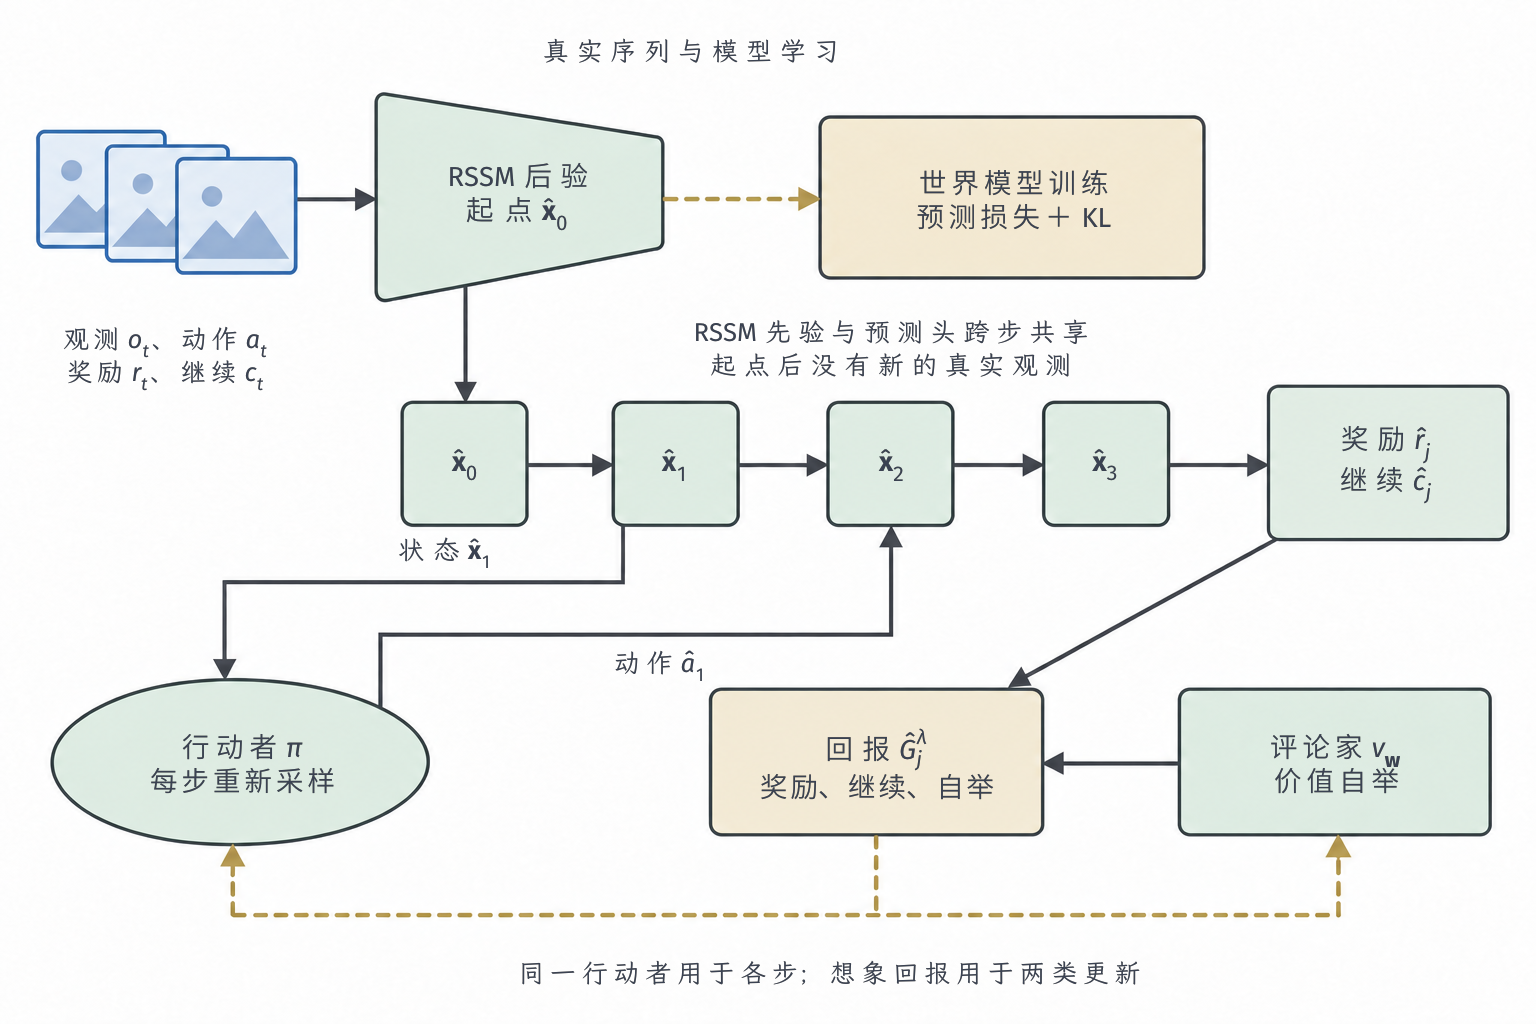
\includegraphics[width=157.400mm]{figures/10-reinforcement-learning/01-problems-and-solving/generated/rl-learning-dreamer/figure.png}
  \caption{RSSM上的真实学习与想象学习。真实序列经后验形成起点并训练世界模型；想象轨迹由先验前进，奖励和继续概率进入回报，价值给出末端自举。部署仍需用新观测更新模型状态，不能把“无逐步搜索”理解为“不再调用模型”。所示潜在格仅解释跨步复用与时序，不固定想象时域或状态维数。}
  \label{fig:rl-learning-dreamer}
\end{figure*}

模型固定后，行动者和评论家需要一个不再依赖未来真实奖励的训练目标。我们从真实后验状态$\widehat{\bm x}_0$开始想象，采样
$\widehat a_j\sim\pi_{\bm\theta}(\cdot\mid\widehat{\bm x}_j)$，再依次得到
$\widehat{\bm x}_{j+1},\widehat r_j,\widehat c_j$。记
$\widehat\gamma_j=\gamma\widehat c_j$为单步有效折扣，长度$L$的$\lambda$回报按逆序递推：
\begin{equation}
 \widehat G_L^\lambda=v_{\bm w}(\widehat{\bm x}_L),\qquad
 \widehat G_j^\lambda
  =\widehat r_j+\widehat\gamma_j
     [(1-\lambda)v_{\bm w}(\widehat{\bm x}_{j+1})
                              +\lambda\widehat G_{j+1}^\lambda].
 \label{eq:rl-learning-dreamer-return}
\end{equation}
例如教学设定$\gamma=0.9,\lambda=0.5,L=2$，两次继续概率均为1，
奖励为$(0.2,0.3)$，后继价值为$(0.4,0.6)$。于是
$\widehat G_1^\lambda=0.84$，
$\widehat G_0^\lambda=0.758$。若第二步继续概率改成0，则相应两值为$0.3$和$0.515$。这说明继续预测错误会同时污染回报与轨迹的有效权重。

Dreamer各版本使用同一训练分工，但不是同一损失。最初版本用连续随机潜变量，并在连续控制中通过模型和评论家反向传播想象回报来训练行动者。DreamerV2改用离散潜变量和直通估计，行动者结合路径导数与似然比估计的方式依动作类型、配置而异\scite{rl3-hafner2020dreamer}

V2的变化使离散视觉控制中的想象学习更实用，但不能据此把后续V3的纯似然比行动者写成相同梯度。V2的网络、目标与评估协议应按其独立论文理解\scite{rl3-hafner2021dreamerv2}

离散潜变量在前向计算中抽出离散取值，抽样操作本身没有通常的连续导数。直通估计（straight-through estimator）在反向计算时用一个连续代理的导数传递梯度，相当于为这一步另定求导规则。它使训练可执行，但一般是有偏估计；不能因为前向样本确实来自离散分布，就将反向代理称为精确导数。区分它与REINFORCE，有助于理解Dreamer不同版本怎样训练行动者。

V3还需处理不同任务的奖励尺度。本书采用2025年Nature正式版的表示：奖励和价值输出固定支撑上的离散概率，而不是直接回归一个标量。取
$b_i=\operatorname{symexp}(u_i)$，
$\operatorname{symexp}(u)=\operatorname{sign}(u)(e^{|u|}-1)$，$u_i$在$[-20,20]$上等距。若目标$y$位于$b_i,b_{i+1}$之间，two-hot目标把概率
$(b_{i+1}-y)/(b_{i+1}-b_i)$和
$(y-b_i)/(b_{i+1}-b_i)$放在相邻两点，其他为0；超出支持范围的值截到边界。训练用该目标与预测分布的交叉熵，读出的均值是$\sum_i p_i b_i$。它是在原始值域插值，不是“先在symlog域求均值，再反变换”的旧式概括。

two-hot编码将目标夹在相邻两点之间的距离转成两个概率，避免只指定最近的一个支撑点。用$\mathcal T(y)$记这一编码，评论家通过最小化它与预测分布的交叉熵拟合停止求导的想象回报，主要项为
\[
  \ell_{\mathrm{critic},j}
    =-\sum_i\mathcal T_i(\operatorname{sg}\widehat G_j^\lambda)
                   \log p_{\bm w,i}(\widehat{\bm x}_j).
\]
这里对软目标取交叉熵。正式版还用EMA评论家输出作正则，并加入真实回放上的辅助价值损失，权重为$0.3$；真实序列的目标利用对应想象起点的在策略回报作标注。这不同于把所有回报自举值统一替换为EMA目标网络。式\eqref{eq:rl-learning-dreamer-return}明确使用当前评论家，监督目标一侧停止梯度。

评论家拟合预测回报后，V3用回报减价值形成行动者优势，并对离散和连续动作均采用归一化的REINFORCE，而非让梯度直接穿过想象动力学。记
$W_j=\prod_{i<j}\widehat\gamma_i$，$c_{\mathrm{ret}}$为想象回报第95与第5百分位差的指数移动平均，则其最大化目标的采样形式为
\begin{equation}
 \sum_{j=0}^{L-1}W_j\left[
   \log\pi_{\bm\theta}(\widehat a_j\mid\widehat{\bm x}_j)
   \operatorname{sg}\left(
       \frac{\widehat G_j^\lambda-v_{\bm w}(\widehat{\bm x}_j)}
            {\max(1,c_{\mathrm{ret}})}\right)
     +\eta\,H(\pi_{\bm\theta}(\cdot\mid\widehat{\bm x}_j))
                       \right].
 \label{eq:rl-learning-dreamer-actor}
\end{equation}
状态、权重和优势在这次行动者更新中作为采样量固定，熵项鼓励而不是惩罚随机性。它从回放起点训练有限想象片段，是实际优化代理，不应声称未经校正就等于真实初始分布目标$J$的精确梯度；因此这里也没有用未归一化的采样和冒充归一化占用期望。

V3正式论文报告多个控制基准上的实验，多数基准使用5个训练种子；Minecraft与BSuite使用10个。Minecraft实验的动作包含抽象合成命令，且有加速破坏方块等协议约定。算法的真实环境证据应连同这些条件解读，不能只把“获得钻石”四字当成跨接口可比的性能单位\scite{rl1-hafner2025-dreamerv3}

表\ref{tab:rl-learning-imagination-cost}说明训练和部署的差别。图\ref{fig:rl-learning-dreamer}中的后验是观测历史的压缩推断，其何时能充当决策状态留给第\ref{chap:rl-information}章；算法把它作为行动者和评论家的潜在状态输入，其充分性需要额外验证。

\begin{table*}[t]
  \centering
  \small
  \begin{tabularx}{\linewidth}{>{\raggedright\arraybackslash}p{24mm} >{\raggedright\arraybackslash}X >{\raggedright\arraybackslash}X}
    \toprule
    阶段 & 模型及策略调用 & 不能省略的成本或检验 \\
    \midrule
    真实序列训练 & 编码观测、后验推断、重建及预测头，梯度更新模型 & 真实交互记录数量、序列长度与反向传播内存 \\
    想象训练 & 多起点先验滚动，逐步调用行动者、奖励、继续与价值头 & 模型转移数、评论家和行动者更新数；高模型回报需真实评估 \\
    部署执行 & 更新循环记忆和观测后验，从策略采样或取约定动作 & 每步状态推断仍有模型成本；随机或确定性评估须预先固定 \\
    在线再学习 & 将新经验写回回放并交替更新三个模块 & 是否允许继续交互、何时更新及更新后状态重算 \\
    \bottomrule
  \end{tabularx}
  \caption{想象学习没有消除模型计算，而是改变了计算发生的位置。部署不做候选轨迹搜索，也不等于一个无状态的策略网络即可运行。}
  \label{tab:rl-learning-imagination-cost}
\end{table*}

% Outline: 3.5.3
\subsection{短模型滚动与离策略优化}
\label{sec:rl-learning-mbpo}

长想象轨迹反复使用模型，错误状态可能继续影响后续奖励和策略输入。基于模型的策略优化（model-based policy optimization, MBPO）这一算法选择另一种折中：从真实回放状态分支，只生成几步经验，写入独立模型缓冲，再混合真实转移记录与模型合成转移训练SAC。它不在这段动力学上直接反传行动者梯度。生成经验的部件与第\ref{sec:rl-learning-dyna}节相同，主要改进对象却是显式行动者；MVE则将短滚动合成一次价值目标，三者不能仅因都用了模型样本就视为相同更新。

记真实缓冲为$D_{\mathrm{real}}$、合成缓冲为$D_{\mathrm{model}}$；每隔$F$个真实环境步拟合一次概率模型集成，每轮抽$B$个真实起点，按当前策略生成至多$k$步。训练批次中真实经验比例为$\eta_{\mathrm{real}}$，其余来自合成缓冲。$F,k,B,\eta_{\mathrm{real}}$以及模型合成转移记录保留多久，都影响旧模型和旧策略样本的占比，必须写入配置。图\ref{fig:rl-learning-mbpo}保留了真实转移记录与模型合成转移这两种来源。

\begin{figure*}[t]
  \centering
  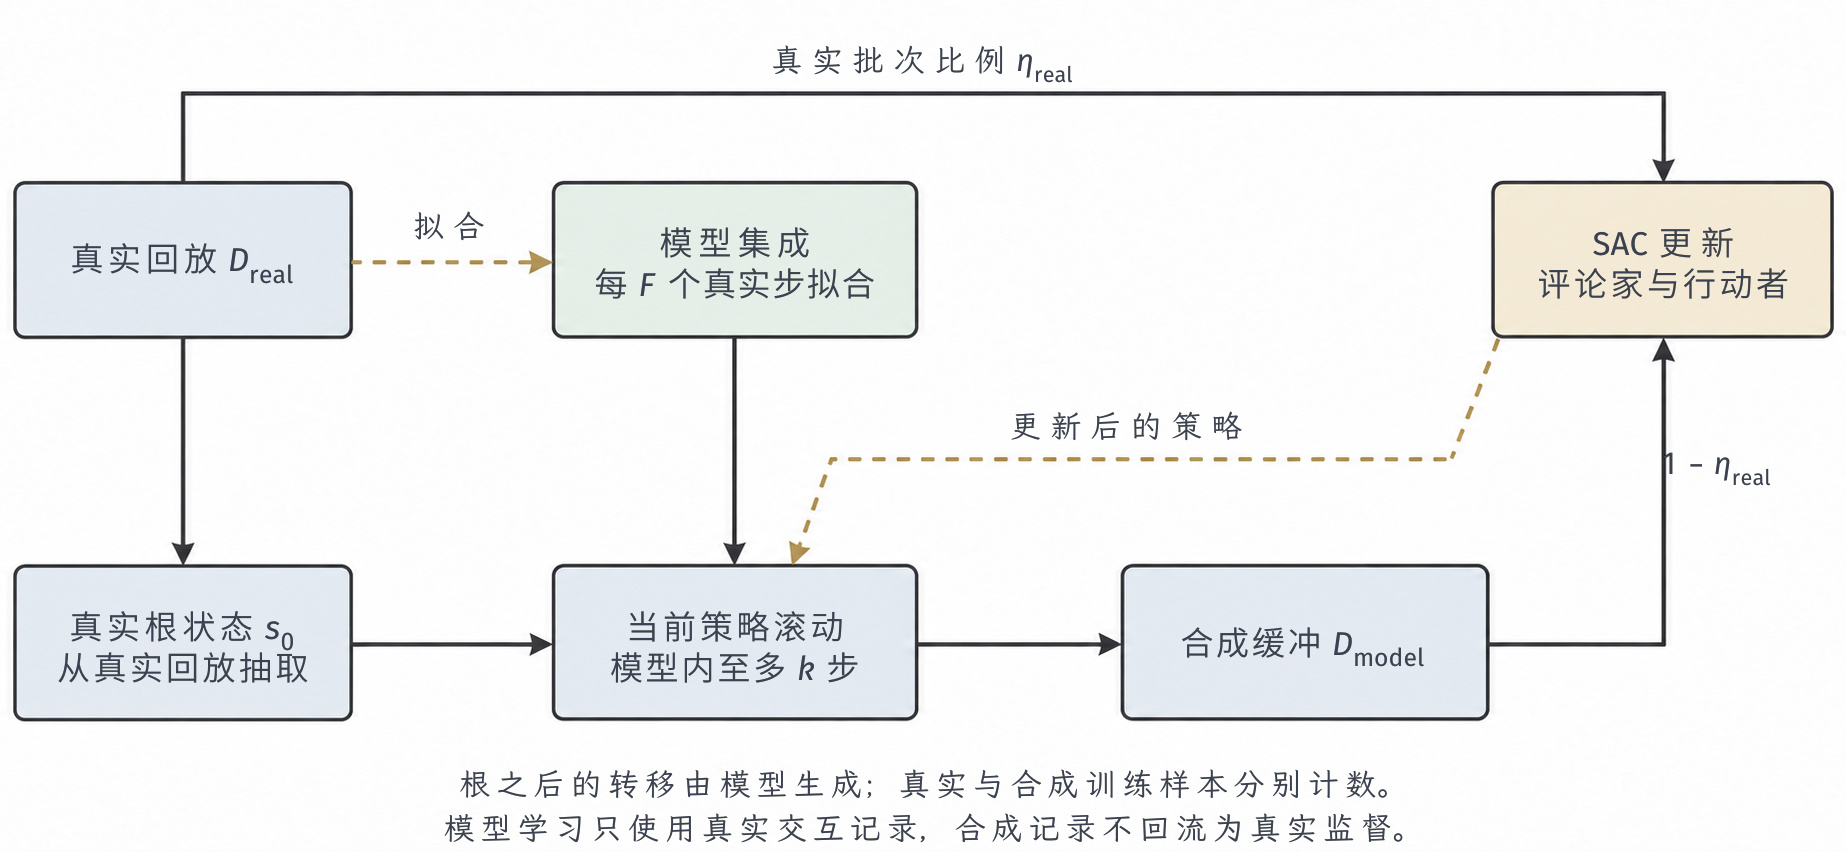
\includegraphics[width=157.400mm]{figures/10-reinforcement-learning/01-problems-and-solving/generated/rl-learning-mbpo/figure.png}
  \caption{MBPO的短分支经验。分支根来自真实回放，根之后的状态、奖励和终止由模型给出；合成缓冲与真实缓冲共同训练SAC。行动者优化时不需要沿动力学反向传播，模型学习仍只以真实交互记录为监督来源。}
  \label{fig:rl-learning-mbpo}
\end{figure*}

一次合成转移可追溯为：从真实记录抽$s=(3,1)$，当前行动者抽到向上，某个集成成员抽到后继$(3,2)$并预测奖励$-0.04$、非终止，于是按$(s,a,r,s',c)$格式把
$((3,1),\text{上},-0.04,(3,2),1)$及模型版本写入模型缓冲，其中$c=1$表示继续。送入采用真实终止字段$z$的SAC回放接口时，须转换为$z=1-c=0$，不能将第五项原样搬入。这一转移在基准网格中可能发生，但本次并没有真的执行；其采样概率取决于所选模型。设后继的SAC目标软值为$0.5$，则这条经验给出的评论家目标仍是$-0.04+0.9\times0.5=0.41$。随后行动者在混合批次的状态上最小化
$\mathbb E[\alpha\log\pi_{\bm\theta}(a\mid s)-\min_iQ_{\bm w_i}(s,a)]$。
这一更新不能因为根是真实状态，就把后继也当成真实观测。

缩短滚动直接减少连续使用错误转移的次数，但也更依赖末端价值。为了量化这项取舍，我们先比较同一起点分布、同一固定策略在真实与学习模型中的$k$步自举评分。设两种分支从$\nu$出发，深度$j$的真实状态动作分布为$q_j^\pi$；以总变差度量后继分布误差，以绝对值度量奖励均值误差，记
\[
 e_T(s,a)=\operatorname{TV}(T(\cdot\mid s,a),\widehat T(\cdot\mid s,a)),
 \qquad e_R(s,a)=|R(s,a)-\widehat R(s,a)|.
\]
假设每个$j<k$都有
$\mathbb E_{q_j^\pi}e_T\leq\epsilon_m$、
$\mathbb E_{q_j^\pi}e_R\leq\epsilon_r$，
两模型奖励均值绝对值不超过$R_{\max}$，并用同一个末端函数$V$且
$\|V\|_\infty\leq V_{\max}$。逐步使用概率核的非扩张性，得到深度$j$的两种状态分布的总变差不超过$j\epsilon_m$。于是两个$k$步自举评分相差至多
\begin{equation}
 B_k=
   \sum_{j=0}^{k-1}\gamma^j
       (\epsilon_r+2R_{\max}j\epsilon_m)
       +2\gamma^kV_{\max}k\epsilon_m.
 \label{eq:rl-learning-short-model-bound}
\end{equation}
奖励误差被分为真实访问处的模型误差与两个访问分布的差，后者乘$2R_{\max}$；末端项同理。若还要与真实无限回报比较，且
$\|V-V^\pi\|_\infty\leq\epsilon_V$，须再加
$\gamma^k\epsilon_V$。短时域降低转移误差累积，却让末端价值误差衰减得更少，不能据此推出$k$越小永远越好。

这个界使用的是目标策略在各深度真实访问处的平均误差，用于评价模型预测误差的转移样本却通常由行为策略$\beta$采集。从$q_j^\beta$转换到$q_j^\pi$，需要知道新策略是否过度访问旧策略轨迹记录很少覆盖的区域。若有
$q_j^\pi(s,a)\leq C_jq_j^\beta(s,a)$，则非负模型误差的期望至多放大$C_j$倍；只知道行为分布上的小均方误差，并不等于已知$\epsilon_m$，更不等于已控制$C_j$。另一种思路是限制
$\sup_s\operatorname{TV}(\pi(\cdot\mid s),\beta(\cdot\mid s))\leq\epsilon_\pi$：
从相同根分布出发，逐步耦合给出策略引起的轨迹分布偏离至多随深度线性增长。MBPO的原始分析正是把训练记录采集策略下的模型总变差误差与策略变化结合，讨论短分支的改进下界；它的抽象单调改进条件不等于实际集成网络加SAC必然单调改进\scite{rl3-janner2019mbpo}

式\eqref{eq:rl-learning-short-model-bound}中的两类转移误差可以按深度理解。第$j$步以前若已有小概率偏离，两种模型就会在不同状态上评分，即使此步各自预测得很准，也可能给不同奖励；这产生$j\epsilon_m$项。末端价值同样受起点之后的偏离影响。把滚动缩短会减少这些项，却让更多未展开回报依赖评论家，这才是短模型滚动的取舍。

若式\eqref{eq:rl-learning-short-model-bound}对整个候选策略集合同时成立，且模型内选择的策略对相应真实目标使用了误差受控的末端值，那么模型代理提升超过两侧总误差才支持真实提升。仅对更新前策略成立的平均验证误差不足以做此推断。表\ref{tab:rl-learning-rollout-controls}列出常用限制各自约束了什么。

\begin{table*}[t]
  \centering
  \small
  \begin{tabularx}{\linewidth}{>{\raggedright\arraybackslash}p{25mm} >{\raggedright\arraybackslash}X >{\raggedright\arraybackslash}X}
    \toprule
    设计 & 直接作用 & 仍未保证的条件 \\
    \midrule
    从真实回放分支 & 避免从模型生成的长历史起步 & 根可能来自旧策略；根之后仍会偏离真实覆盖 \\
    限制$k$并调整日程 & 减少连续使用错误转移的次数 & 不证明末端价值准确，也不证明给定长度最优 \\
    提高真实批次比例 & 减少当前更新中合成转移记录的权重 & 不能补出真实交互记录未覆盖的动作 \\
    集成分歧筛选 & 排除模型成员明显不一致的转移 & 成员可能共同犯错；分歧不是经校准的TV半径 \\
    限制合成转移记录的保留时间 & 降低旧模型生成经验的占比 & 当前模型仍可能有系统性偏差 \\
    \bottomrule
  \end{tabularx}
  \caption{短模型滚动的控制量与边界。它们是需要验证的算法设计，不是全局性能或安全证明。}
  \label{tab:rl-learning-rollout-controls}
\end{table*}

% Outline: 3.5.4
\subsection{模型误差下的策略优化边界}
\label{sec:rl-learning-model-policy-boundary}

不做部署搜索并不能避免模型利用偏差，模型梯度同样会把行动者引向高估区域。设一个独立的一步连续动作教学任务为$a\in[-1,1]$、真实奖励$R(a)=-a^2$，模型奖励
$\widehat R(a)=-a^2+0.8a$。真实训练记录若只包含执行$a=0$后的奖励反馈，模型在那里误差为0；从确定性策略$a=\theta=0$出发，模型梯度却是$0.8$。它最终把动作推到$0.4$，预测奖励$0.16$，真实奖励$-0.16$，而原策略真实奖励为0。这个例子不涉及长时域误差，已经足以说明“多做模型内策略更新”可能降低真实性能。

上例的旧策略只访问$a=0$，模型评价该策略完全准确；优化却选出了旧策略交互记录从未验证的$a=0.4$。因此，从固定策略评估扩大到模型内选策略时，误差控制也要扩大到候选策略会到达的区域，或由对依据训练记录选出的策略也同时有效的置信集合承担这一要求。第\ref{sec:rl-learning-model-bias}节的统一模拟界可支持选择后的回报结论，单点拟合则不能。图\ref{fig:rl-learning-model-feedback}展示策略改变访问分布后需要补充真实验证的反馈，表\ref{tab:rl-learning-model-policy-errors}列出处置位置与代价。

\begin{figure*}[t]
  \centering
  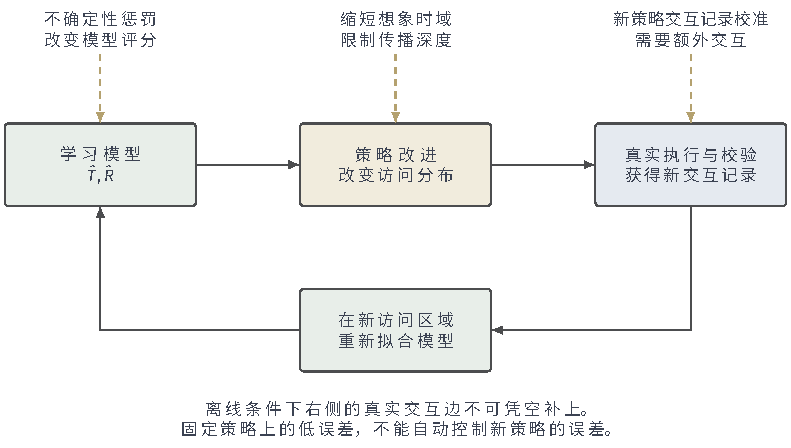
\includegraphics[width=133.960mm]{figures/10-reinforcement-learning/01-problems-and-solving/tikz/rl-learning-model-feedback.pdf}
  \caption{模型策略优化中的访问分布反馈。虚线标明三种限制分别作用的位置；补充真实转移记录要求仍有交互能力，离线训练不能假定这条边随时可用。上例中的模型梯度把策略从已验证的$a=0$推向未验证区域。}
  \label{fig:rl-learning-model-feedback}
\end{figure*}

\begin{table*}[t]
  \centering
  \small
  \begin{tabularx}{\linewidth}{>{\raggedright\arraybackslash}p{26mm} >{\raggedright\arraybackslash}X >{\raggedright\arraybackslash}X}
    \toprule
    误差处置 & 主要限制的环节 & 代价及不足 \\
    \midrule
    不确定性惩罚 & 用$\widehat R-\lambda u$降低未确信区域的代理收益 & 需要$u$对相关错误敏感；可能过度保守、阻碍必要探索 \\
    缩短想象时域 & 减少模型误差传播深度 & 更依赖末端评论家，可能漏掉延迟后果 \\
    真实转移记录校准 & 在新策略访问处验证并更新模型 & 需要额外交互；不可逆损失不能靠事后校准撤销 \\
    限制策略变化 & 避免单次更新过快远离支持区域 & 局部变化小仍可累积成大偏离，旧覆盖不永久有效 \\
    \bottomrule
  \end{tabularx}
  \caption{模型误差措施并不互相替代。惩罚改变评分，短时域改变传播，真实校准增加新策略访问处的转移记录；三者对应不同的误差来源。}
  \label{tab:rl-learning-model-policy-errors}
\end{table*}

动作条件视频模型将预测对象扩大到画面序列，但策略训练仍依赖动作后果是否正确。生成画面可以逼真，却错误地预测“按下这个键便到达门口”。判断其能否支持策略训练，需核对动作接口、视频与动作记录是否覆盖所需干预、奖励和终止的来源、部署能否闭环接收观测，以及真实环境测试结果。开放环视频质量评价观测预测，不能单独继承为闭环回报保证。

\Needspace{20\baselineskip}
Dreamer 4提供了一个具体延伸案例。这里讨论的是2025年9月29日发布的原始预印本版本\scite{rl1-hafner2025-dreamer4}
它使用VPT承包者提供的2541小时、360p、20帧每秒的Minecraft视频及键鼠和事件记录；动作接口包含23个二元按键与121类鼠标动作。模型内学习使用任务嵌入，测试有预设任务提示序列。使用这些视频、动作和事件记录的训练是离线的；即便模型内策略采样是同策略，也不意味着算法在真实环境中在线采集新的训练记录。

该版本报告在1000个随机世界、空背包、每回合60分钟的真实Minecraft测试中，获得钻石的成功率为$0.7\%$。这是闭环环境证据，强于只展示视频，却仍受动作接口、任务提示和视频、动作及事件记录的来源限制；它既不是DreamerV3抽象动作协议下的直接同预算比较，也不是机器人安全保证。模型速度、生成质量和策略成功率应分开报告。

至此，模型的用途已能按真实交互记录、模型预测与更新目标之间的依赖区分：Dyna把模拟转移用于价值备份，MPC与MuZero用模型进行当前决策搜索，Dreamer把想象轨迹用于策略训练，MBPO把短合成转移交给离策略行动者—评论家。一个系统可以同时拥有这些部件；判断其条件，应看真实交互记录如何进入、哪项预测参与了哪次更新，以及最终动作究竟由谁给出。

% Outline: 3.6
\section{时间抽象下的价值与策略学习}
\label{sec:rl-learning-temporal-abstraction}

前述更新默认每步选择一个原子动作。在房间导航中，一段“走到门口”的控制过程可以重复调用，高层不必每步重新选方向。时间抽象（temporal abstraction）把这段持续行为当作一次决策，改变的是决策间隔，而不是是否使用模型或是否优化显式策略。因此它可分别与四种求解组合结合，也仍需要学习内部动作、评价长期回报和取得覆盖相关状态动作的交互记录。

% Outline: 3.6.1
\subsection{时间抽象解决什么问题}
\label{sec:rl-learning-temporal-purpose}

考虑一个完全可观测、突出房间结构的独立确定性教学网格，区别于前文$4\times3$基准：格点为
$x=1,\ldots,8$、$y=1,\ldots,5$；$x=4$与$x=5$之间有墙，仅在$y=2,4$开门。上下左右每步确定移动一格，不合法动作不可选。起点为$(2,2)$、目标为$(7,2)$，入目标奖励1，其余步$-0.04$，$\gamma=0.9$。图\ref{fig:rl-learning-options-rooms}画出原子动作与高层决策的对应。

从起点到目标的最短路线仍需五个原子动作。若预先可调用两步的“到下门左侧$(4,2)$”和三步的“穿下门并到目标”，高层只选择两次，执行层却仍与环境交互五步。时间抽象节省的是高层决策深度：在更大房间中，探索可以保持一段有方向的行为，回报也可评价整个子任务。要取得这些收益，内部控制必须能完成调用，终止规则必须在适当时刻交回控制权；两者本身也有学习代价。

\begin{figure*}[t]
  \centering
  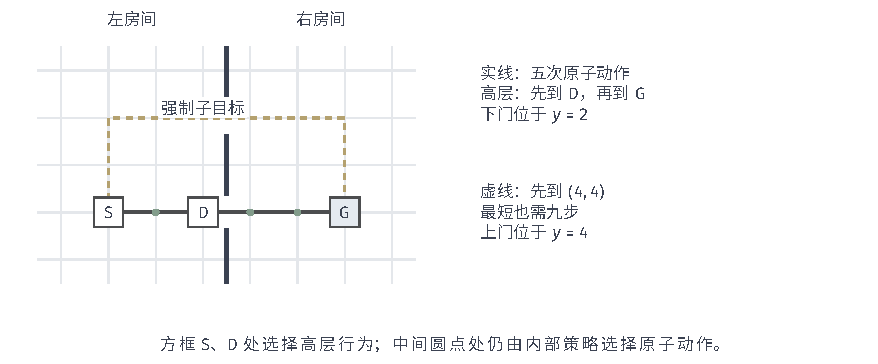
\includegraphics[width=148.749mm]{figures/10-reinforcement-learning/01-problems-and-solving/tikz/rl-learning-options-rooms.pdf}
  \caption{两房间教学网格中的时间抽象。实线路径有五个原子动作，可由两次高层调用组成；虚线路径强制经过上门左侧，多走四步。圆点表示原子时刻，方框标出高层选择时刻。图中几何与奖励规则均为独立教学设定。}
  \label{fig:rl-learning-options-rooms}
\end{figure*}

动作的取值形式与持续时间是两个维度。机器人每毫秒选择一次实数力矩，虽是连续动作，仍是原子决策；“沿墙前进直到门口”可以只有一个离散编号，却持续随机多步。时间抽象本身不改变外在奖励目标，也不承诺内部执行满足安全约束。若为了训练低层另外奖励“接近门口”，还须说明这是辅助目标，以及它是否可能与全局目标冲突。

\begin{table*}[t]
  \centering
  \small
  \begin{tabularx}{\linewidth}{>{\raggedright\arraybackslash}p{24mm} >{\raggedright\arraybackslash}X >{\raggedright\arraybackslash}X}
    \toprule
    职责 & 输入与输出 & 需要指定或学习的对象 \\
    \midrule
    高层选择 & 状态、任务$\to$行为编号或子目标 & 高层策略、每个行为的价值及可启动条件 \\
    内部控制 & 当前状态、行为或子目标$\to$原子动作 & 低层策略，必要时用子任务奖励训练 \\
    终止判定 & 当前状态、行为$\to$是否交还控制 & 终止概率、超时或到达条件；超时不必等于环境终止 \\
    \bottomrule
  \end{tabularx}
  \caption{时间抽象的三个学习对象。手工规则与自动发现是获得这些对象的不同方式，不改变它们各自的职责。}
  \label{tab:rl-learning-hierarchy-objects}
\end{table*}

表\ref{tab:rl-learning-hierarchy-objects}也指出为什么“给动作起一个高层名字”还不够：必须知道在何处可执行、执行期间如何行动、多久返回。只有这些条件明确，才能把一段行为当作新的动作参与备份。

% Outline: 3.6.2
\subsection{半马尔可夫决策与Options}
\label{sec:rl-learning-options}

调用“到门口”后，下一次高层决策可能在两步后，也可能因绕行在更晚发生。高层因此要同时记录终点、期间奖励和持续时间，不能继续把每次调用当成原来的一步动作。半马尔可夫决策保留这三种随机后果；Option则用启动条件、内部动作策略和终止规则描述一个可调用行为。

\begin{example}[持续时间不能忽略]
  \label{ex:rl-learning-option-duration}
  在房间网格的$(4,2)$到$(6,2)$，Option A走两步，Option B先绕行再用四步到同一终点；期间不碰最终目标，奖励均为$-0.04$。假设终点价值为$0.8$，则
  \[
    y_A=-0.04(1+0.9)+0.9^2(0.8)=0.572,
  \]
  \[
    y_B=-0.04(1+0.9+0.9^2+0.9^3)+0.9^4(0.8)=0.38732.
  \]
  若错误地都只折扣一次，目标变为$0.644$与$0.58244$，两者都被高估。持续时间随机时应平均$\gamma^K V(s_{t+K})$，一般不能换成$\gamma^{\mathbb E K}\mathbb E V$。
\end{example}

\begin{definition}[半马尔可夫决策与Markov Option]
  \label{def:rl-learning-option}
  在离散原子时间上，设高层决策时刻为$t_0<t_1<\cdots$，每次持续时间$K_j=t_{j+1}-t_j$为正整数。若给定当前决策状态$s_{t_j}$及所选高层动作后，下一决策状态、期间累计奖励与$K_j$的联合条件律不再依赖更早历史，则称该决策过程为半马尔可夫决策过程。一个Markov Option记为
  $\omega=(I_\omega,\pi_\omega,\beta_\omega)$：
  $I_\omega\subseteq S$是启动集，
  $\pi_\omega(a\mid s)$是内部原子动作策略，
  $\beta_\omega(s)\in[0,1]$是在到达$s$后终止的概率。
  一次调用先执行至少一个原子动作，再根据到达状态检测是否终止；启动条件、内部策略和终止概率只依赖当前状态和Option编号。高层策略$\zeta(\omega\mid s)$只在允许启动的Option中选择。
\end{definition}

“半马尔可夫”保留了决策时刻的状态条件性，但决策间隔不再固定为一步，因此持续时间也进入后果分布。启动集说明在哪些状态能调用，内部策略说明调用期间每步做什么，终止规则说明何时把控制交回高层；缺少其中一项，就不能确定这段行为对应的奖励、终点与时长。这里的$\beta_\omega$专指Option终止概率，与前面行为策略$\beta$的对象不同，下标$\omega$用于区分。

在固定内部策略和终止规则下，起点$s$与Option$\omega$决定终点及持续时间的分布，这正是半马尔可夫模型。原子动作也可保留：令其内部只执行该动作一次并立即终止，即得到持续时间$K=1$的Option。若Option依赖内部记忆或已执行时长，需把所需变量并入状态，不能继续无条件使用上述Markov形式。Options框架将这种多步行为与原有MDP的价值学习连接起来\scite{rl3-sutton1999options}

为了仍评价原任务的折扣回报，我们按一次Option的实际执行边界分组，而不按高层调用次数重新计时。设调用从$t$执行至$t+K$，前$K$步奖励归入本次行为，余下回报从$t+K$开始；逐项写出便有
\begin{align}
 G_t
   &=r_t+\gamma r_{t+1}+\cdots+\gamma^{K-1}r_{t+K-1}
          +\gamma^K(r_{t+K}+\gamma r_{t+K+1}+\cdots)\notag\\
   &=R_t^\omega+\gamma^K G_{t+K},\qquad
 R_t^\omega:=\sum_{j=0}^{K-1}\gamma^j r_{t+j}.
 \label{eq:rl-learning-option-grouping}
\end{align}
这个等式对每次持续时间有限的Option调用成立，再按给定$s_t=s,\omega_t=\omega$的分布取期望，就有
\begin{equation}
 Q^\zeta_\Omega(s,\omega)
  =\mathbb E\left[
       R_t^\omega+\gamma^K
          \sum_{\omega'}\zeta(\omega'\mid s_{t+K})
                       Q^\zeta_\Omega(s_{t+K},\omega')
                    \,\middle|\,s,\omega\right].
 \label{eq:rl-learning-option-bellman}
\end{equation}
因此高层回放至少应保存$(s_t,\omega,R_t^\omega,K,s_{t+K})$与环境终止标志。若终点是环境吸收终止，后继值为0；Option主动结束只是把控制权交回高层，后继值通常不为0。

评价固定高层策略时按$\zeta$平均下一Option；改为控制时，则在下一状态允许启动的$\Omega(s_{t+K})$中取最高估值，以改进后续高层选择。样本更新为
\[
 Q_\Omega(s_t,\omega)\leftarrow Q_\Omega(s_t,\omega)+
  \alpha\left[R_t^\omega+
        \gamma^K\max_{\omega'\in\Omega(s_{t+K})}
                          Q_\Omega(s_{t+K},\omega')
                     -Q_\Omega(s_t,\omega)\right].
\]
把$\gamma^K$写成$\gamma$相当于用高层调用次数重新定义时间，会改变原始任务，而不是同一个目标下的近似实现。

\begin{theorem}[Option备份的压缩性]
  \label{thm:rl-learning-option-contraction}
  设$S$有限，每个非终止状态的可启动Option集$\Omega(s)$有限且非空，原子奖励有界，$0\leq\gamma<1$。固定各Option的内部策略和终止规则，每次调用的持续时间$K\geq1$且几乎处处有限。设$\zeta(\cdot\mid s)$是在$\Omega(s)$上归一的合法平稳高层策略。对有界状态价值函数$V$，定义
  \[
    \begin{aligned}
    (\mathcal B_\Omega^\zeta V)(s)
       &=\sum_{\omega\in\Omega(s)}\zeta(\omega\mid s)
          \mathbb E[R_t^\omega+\gamma^K V(s_{t+K})\mid s,\omega],\\
    (\mathcal B_\Omega^*V)(s)
       &=\max_{\omega\in\Omega(s)}
          \mathbb E[R_t^\omega+\gamma^K V(s_{t+K})\mid s,\omega].
    \end{aligned}
  \]
  两算子在终止状态都定义为0，调用结束于终止状态时的后继价值也取0。对任意有界$V,W$及$\mathcal B\in\{\mathcal B_\Omega^\zeta,\mathcal B_\Omega^*\}$，有
  $\|\mathcal BV-\mathcal BW\|_\infty\leq\gamma\|V-W\|_\infty$。
\end{theorem}

\begin{proof}
  固定$s,\omega$，累计奖励在两次备份相减时抵消，余项绝对值至多为
  \[
    \mathbb E[\gamma^K|V(s_{t+K})-W(s_{t+K})|\mid s,\omega]
      \leq\mathbb E[\gamma^K\mid s,\omega]\|V-W\|_\infty
      \leq\gamma\|V-W\|_\infty.
  \]
  高层概率平均不增大此界；最大值满足
  $|\max_\omega x_\omega-\max_\omega y_\omega|
       \leq\max_\omega|x_\omega-y_\omega|$，故同样成立。对$s$取上确界即得结论。
\end{proof}

固定内部策略和终止规则后，备份误差只来自终点价值，因而实际持续时间越长，这一误差的折扣越强；压缩因子可以收紧为$\sup_{s,\omega}\mathbb E[\gamma^K\mid s,\omega]$。这里取上确界是要覆盖每个可启动状态与Option，并不说明获得长行为的训练样本更少。若Option可能永不终止，原始折扣回报仍可能有定义，但下一高层决策时刻不再总是有限；需要另行规定该事件上的回报与备份，不能直接使用上述陈述。在有界状态价值函数的一致范数空间中，空间完备，且有界奖励使这两个备份仍输出有界函数。它们因此各有唯一不动点，反复应用同一备份会按压缩率收敛；这个结论只用于固定Option集合及内部规则的价值求解。

% Outline: 3.6.3
\subsection{分层价值与策略学习}
\label{sec:rl-learning-hierarchical-learning}

Option备份暂时固定了内部策略和终止规则，接下来要决定怎样获得它们。手工指定“到下门”时，低层读取当前格点和门位置，输出方向，并可用到门奖励训练；高层读取当前房间和外在任务，选择子目标，仍以原始折扣奖励评价。如果不预先指定门位置，Option-Critic可以直接用外在回报训练内部策略及终止概率。图\ref{fig:rl-learning-hierarchy}区分各层输入、动作与奖励，避免把低层辅助目标混成全局任务。

\begin{figure*}[t]
  \centering
  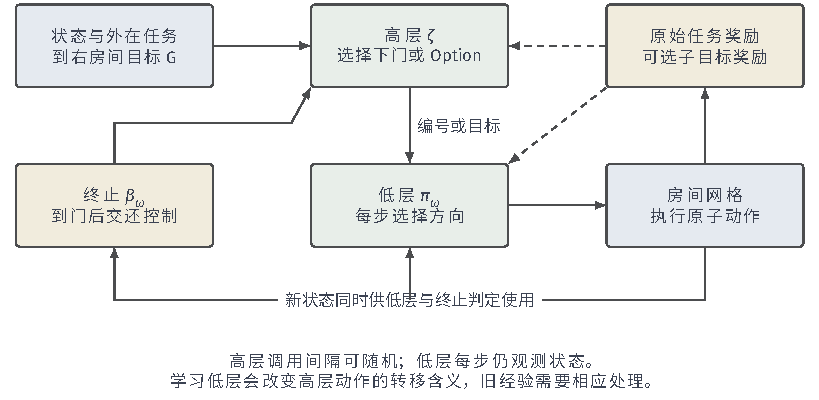
\includegraphics[width=138.747mm]{figures/10-reinforcement-learning/01-problems-and-solving/tikz/rl-learning-hierarchy.pdf}
  \caption{房间任务的分层接口。高层交付子目标或Option编号，低层持续输出原子动作，终止后才交回控制权。右侧区分原始任务奖励与可选的低层辅助奖励；Option-Critic无需人为指定这一辅助奖励。}
  \label{fig:rl-learning-hierarchy}
\end{figure*}

内部规则若也要学习，高层看见的“同一个Option”会随训练改变。过去两步能到门口的调用，今天可能更快，也可能绕行；旧高层记录中的终点和时长未必仍代表当前低层。因此先建立固定内部规则的备份，再讨论联合学习和旧记录校正，有助于分清压缩性究竟针对哪个固定算子。

每个原子步之后既可能继续当前Option，也可能终止并重选，所以评价还需保留当前Option编号。Option-Critic为这两种后续选择分别估值。假定所有Option在所有非终止状态均可启动，记$Q_\Omega(s,\omega)$为当前继续执行$\omega$的价值，
$V_\Omega(s)=\sum_{\omega'}\zeta(\omega'\mid s)Q_\Omega(s,\omega')$为重新选择的价值。到达$s'$后，尚未作终止选择的价值是
\begin{align}
 U(\omega,s')
   &=(1-\beta_\omega(s'))Q_\Omega(s',\omega)
                               +\beta_\omega(s')V_\Omega(s'),\notag\\
 Q_U(s,\omega,a)
   &=R(s,a)+\gamma\mathbb E_{s'\sim T(\cdot\mid s,a)}U(\omega,s'),\notag\\
 Q_\Omega(s,\omega)&=\sum_a\pi_\omega(a\mid s)Q_U(s,\omega,a).
 \label{eq:rl-learning-option-critic}
\end{align}
这些关系允许每个原子步更新评论家，而不必等Option结束。采样转移的目标是
$y=r_t+\gamma U(\omega_t,s_{t+1})$，环境终止时令$U=0$；内部策略则提高$Q_U$大的动作的概率。

固定高层$\zeta$及终止参数，用$\bm\theta$参数化内部策略。定义当前执行状态与Option的归一化占用
$d_\Omega(s,\omega)=(1-\gamma)\sum_{t\geq0}\gamma^t
\mathbb P(s_t=s,\omega_t=\omega)$。环境终止后以零奖励吸收态和固定虚拟Option延拓，使占用总质量仍为1；该延拓不贡献参数梯度。将普通策略梯度应用于包含Option的扩展过程，可得
\begin{equation}
 \nabla_{\bm\theta}J
   =\frac{1}{1-\gamma}
     \mathbb E_{(s,\omega)\sim d_\Omega,\ a\sim\pi_\omega}
       [\nabla_{\bm\theta}\log\pi_\omega(a\mid s)
                                    Q_U(s,\omega,a)].
 \label{eq:rl-learning-intra-option-gradient}
\end{equation}
基线$Q_\Omega(s,\omega)$与动作无关，可以减去以形成内部优势。推导中的占用仍按原子时间折扣，而不是每切换一次Option才折扣。

终止规则的方向可直接从$U$看出。若$\bm\nu$参数化$\beta$，对终止概率的局部导数是
$V_\Omega(s')-Q_\Omega(s',\omega)=-A_\Omega(s',\omega)$。展开未来各次到达的影响，得到
\begin{equation}
 \nabla_{\bm\nu}J
   =-\sum_{t\geq0}\gamma^{t+1}
       \mathbb E[
          \nabla_{\bm\nu}\beta_{\omega_t}(s_{t+1})
                          A_\Omega(s_{t+1},\omega_t)].
 \label{eq:rl-learning-termination-gradient}
\end{equation}
前面的$\gamma$来自先走一步再决定终止。若将到达分布
$(1-\gamma)\sum_t\gamma^t\mathbb P(s_{t+1},\omega_t)$归一化，上式系数就是$-\gamma/(1-\gamma)$。当前Option比重新选择更好时$A_\Omega>0$，梯度会降低终止概率；较差时则提高。高层策略本身若也需求导，应另计高层选择时刻的贡献，不能藏进这个固定$\zeta$的偏导。完整的策略与终止梯度关系见Option-Critic原论文\scite{rl3-bacon2017optioncritic}

例如人工评价值为$Q_\Omega(s',\omega)=0.6$、
$V_\Omega(s')=0.9$，当前$\beta=\sigma(\nu)=0.25$，则
$U=0.675$。前一步奖励$-0.04$、$\gamma=0.9$时，评论家目标为$0.5675$。终止logit的局部上升方向为
$-\beta(1-\beta)A_\Omega=0.05625$；把它乘对应到达折扣权重后，提高终止概率。这一方向不是“价值低就终止”，而是“继续比切换更差就终止”。

其他分层方法主要改变任务分解与交互记录复用方式，不能简单替换上述三个学习对象。Feudal RL用管理者向下层发指令，由下层完成指令获取局部奖励；状态划分与层级接口提供了强先验，也限制了能表达的行为\scite{rl3-dayan1993feudal}

MAXQ把任务写成子任务图，将“执行子任务本身的价值”与“完成它以后还剩多少价值”分开。若在父任务$i$中选择子任务$a$，完成后用$C_i(s,a)$表示父任务剩余部分，则决策评价具有
$Q_i(s,a)=V_a(s)+C_i(s,a)$的结构，完成项包含子任务持续时间的折扣。它学习的是给定分解下的价值；递归最优只要求每个子任务在固定子层下最优，比原始MDP全局最优弱\scite{rl3-dietterich2000maxq}

HIRO用高层给出的相对目标$\bm g_t$训练低层。这里改用连续状态坐标$\bm s_t\in\mathbb R^{d_s}$表示$s_t$，目标也是这组坐标中的位移向量，不通过学习编码重新定义目标距离。高层每$c$个原子步提出一次目标，$c$为固定正整数；窗口内低层以状态与相对目标为输入，并用负距离$-\lVert\bm s_i+\bm g_i-\bm s_{i+1}\rVert_2$作为辅助奖励。令$\bm g_{i+1}=\bm s_i+\bm g_i-\bm s_{i+1}$，便使绝对目的地$\bm s_i+\bm g_i$在窗口内不变。

低层更新会使旧高层动作失去原意：过去“向东两格”的目标现在可能对应另一串原子动作。重标记时保持已经观察的$\bm s_t,\ldots,\bm s_{t+c}$与$a_t,\ldots,a_{t+c-1}$不变，改变的只是起始目标。原实现从10个候选中搜索：旧目标、实际端点位移$\bm s_{t+c}-\bm s_t$，以及8个以该位移为中心的高斯提议。高层接口规定目标各坐标的上下界；高斯提议的各坐标标准差取对应允许范围的四分之一，并裁剪回该范围。这是有限候选近似，不是对任意目标求精确全局最大值。

对每个候选$\widetilde{\bm g}_t$，逐步相对目标由
$\widetilde{\bm g}_i=\bm s_t+\widetilde{\bm g}_t-\bm s_i$，
$i=t,\ldots,t+c-1$确定。用当前含探索噪声的低层行为密度$\pi_{\mathrm{low}}$计算
$\sum_{i=t}^{t+c-1}\log\pi_{\mathrm{low}}
(a_i\mid s_i,\widetilde{\bm g}_i)$，
选择评分最高的候选重标高层经验。在固定各向同性高斯动作噪声下，这相当于最小化记录动作与当前低层均值动作的平方距离和。它校正的是低层行为变化，不是把未发生的真实轨迹补出来\scite{rl3-nachum2018hiro}

HAC则把实际达到的状态作为事后高层动作，并在各层做目标重标记，以近似“下层已经能完成这个动作”的训练接口；另外安排子目标测试，对当前低层不能完成的提议施加相应惩罚。只使用成功的事后重标记、忽略测试，会让上层把不可达子目标估得过高\scite{rl3-levy2019hac}

\begin{table*}[t]
  \centering
  \small
  \begin{tabularx}{\linewidth}{>{\raggedright\arraybackslash}p{22mm} >{\raggedright\arraybackslash}X >{\raggedright\arraybackslash}X}
    \toprule
    方法 & 预先给定的结构 & 学习对象与交互记录复用难点 \\
    \midrule
    Feudal RL & 管理层级、状态抽象与指令接口 & 各层指令选择和执行策略；局部奖励可能限制全局行为 \\
    MAXQ & 子任务图、终止条件及可能的伪奖励 & 子任务值与完成项；保证依赖任务分解和状态抽象条件 \\
    Option-Critic & Option数量、参数化及启动约定 & 内部策略、终止与高层价值；可能退化为过短或重复Option \\
    HIRO & 目标坐标、执行窗口、距离奖励 & 高低层离策略策略；用当前低层动作似然校正旧目标 \\
    HAC & 各层目标空间、执行预算及测试机制 & 多层目标策略；事后动作、事后目标和子目标测试分工不同 \\
    \bottomrule
  \end{tabularx}
  \caption{分层方法的先验与学习边界。表中层级都需要明确的状态、目标、动作和奖励接口，不是把同一个单层算法重复堆叠即可。}
  \label{tab:rl-learning-hierarchy-methods}
\end{table*}

表\ref{tab:rl-learning-hierarchy-methods}所列先验可能降低学习难度，也可能排除好策略。在图\ref{fig:rl-learning-options-rooms}中，若所有高层策略都被强制先到$(4,4)$，最短路线从五步变为九步。对应回报分别是
$-0.04\sum_{j=0}^{3}0.9^j+0.9^4=0.51854$和
$-0.04\sum_{j=0}^{7}0.9^j+0.9^8\approx0.20265$。
即使每个子任务都学得完美，仍无法恢复被层级排除的下门直达路线。若同时保留全部原子动作且允许高层任意选择，它仍可表示原始最优策略，但搜索和学习未必会及时找到它。

% Outline: 3.6.4
\subsection{技能发现与下游复用}
\label{sec:rl-learning-skill-discovery}

手工指定门口已经利用了下游任务知识。没有外在奖励时，可以先训练一组产生不同可控后果的行为，随后检验它们能否被任务策略调用。先考虑取有限标签的\term{技能变量}$Z\in\{1,\ldots,m_Z\}$。固定起点$s_0$与执行时域或终止规则后，先按先验$p(z\mid s_0)$抽取标签，再从$s_0$执行技能策略$\pi(a\mid s,z)$，由策略与环境共同产生后果$Y$。$Y$可取终点、访问状态或轨迹摘要；上述抽样与执行过程共同规定$(Z,Y)$的联合律。判别器$q_{\bm\psi}(z\mid y,s_0)$从后果反推技能。不同技能若总到同一处便难以区分；若差别仅来自不可控噪声，也难以由技能稳定产生。这里希望学习的是选择行为可以改变的后果。

在房间任务中，可以让技能1趋向左下、技能2趋向左上，再训练判别器从终点判断用了哪个技能。如果两个技能总到同一处，终点不能提供辨认技能标签的证据；如果终点区域互不重叠，观察终点就能识别标签。互信息（mutual information）量化这种平均辨识收益：看到行为后果以后，对所选技能还有多少不确定性，比看到后果以前减少了多少。下面比较的是技能标签与后果的联合分布，不是单独追求后果越随机越好。

固定起点$s_0$和执行时域或终止规则。对每个技能$z$，令$Q_z(\mathrm dy\mid s_0)$为执行策略$\pi_z$后、由环境转移及所选轨迹摘要共同生成的后果分布；假设后果空间为标准Borel空间。先验满足$p(z\mid s_0)>0$且$\sum_zp(z\mid s_0)=1$，因此联合律明确为
\[
 P(Z=z,Y\in B\mid s_0)=p(z\mid s_0)Q_z(B\mid s_0).
\]
用联合律与边缘律乘积的KL比较技能选择与后果的依赖，得到
\[
 \begin{aligned}
 I(Z;Y\mid s_0)
 &=D_{\mathrm{KL}}\!\left(P_{Z,Y\mid s_0}\,\middle\|\,
          P_{Z\mid s_0}\otimes P_{Y\mid s_0}\right)\\
 &=\mathbb E\log\frac{p(Z\mid Y,s_0)}{p(Z\mid s_0)}\\
 &=H(Z\mid s_0)-H(Z\mid Y,s_0).
 \end{aligned}
\]
最后两项只对有限技能标签的先验与后验概率求Shannon熵，均有限；自然对数的单位为nat。因此$0\leq I(Z;Y\mid s_0)\leq\log m_Z$，其含义是观察后果平均减少了多少技能不确定性。$Y$可以离散、连续或混合，不能改用$Y$的两个可能无限的熵相减。连续技能等一般变量仍使用联合律的KL表达，互信息可能为无穷，熵差须另查有限性。

赋能（empowerment）用信道容量表达可区分的控制选择。例如，设原子动作集有限且在所有相关状态可用，固定执行长度$K\geq1$；预先选定一个开环动作序列，由环境生成末端状态$S_K$。对允许的序列分布优化，容量为
\[
 \max_{p(a_{0:K-1}\mid s_0)}
       I(A_{0:K-1};S_K\mid s_0).
\]
候选分布仅给合法可执行的序列分配质量。用根据途中观测调整动作的闭环技能替代开环序列，会改变允许的控制类；有限技能目标与这种容量不能直接视为同一个优化问题。

\begin{example}[后果随机，技能仍可完全区分]
  \label{ex:rl-learning-finite-skill-mi}
  在一维位置教学任务中，两个技能以各$1/2$的概率被选取。技能1停在位置0，技能2的终点在$[1,2]$上均匀分布。看见终点便能确定执行了哪个技能，所以$H(Z)=\log2$、$H(Z\mid Y)=0$，互信息为$\log2$。技能2的具体落点仍有随机性，但这不妨碍识别技能。此时$Y$同时含有点质量与连续部分，直接套用普通离散熵或微分熵的差并不合适；有限标签$Z$的熵差仍有明确含义。
\end{example}

计算互信息需要技能与后果的联合分布，但真实后验$p(z\mid y,s_0)$通常不能直接计算。以下仍以有限标签说明，并假设判别器给真实技能的概率为正、有关对数项可积。判别器给出一个可由带技能标签的交互记录拟合的替代概率；用它构造下界，策略就有可计算的训练信号。在互信息的对数比中加减$\log q_{\bm\psi}$，有
\begin{align}
 I(Z;Y\mid s_0)
   &=\mathbb E\left[\log q_{\bm\psi}(Z\mid Y,s_0)
                                  -\log p(Z\mid s_0)\right]\notag\\
   &\quad+\mathbb E_Y D_{\mathrm{KL}}
       (p(\cdot\mid Y,s_0)\|q_{\bm\psi}(\cdot\mid Y,s_0))\notag\\
   &\geq\mathbb E\left[\log q_{\bm\psi}(Z\mid Y,s_0)
                                  -\log p(Z\mid s_0)\right].
 \label{eq:rl-learning-skill-mi}
\end{align}
判别器用带已知技能标签的经验做最大似然训练；策略把括号内的量当作内部奖励。这一推导只用KL非负性，但所得到的学习质量仍取决于后果选择、判别器容量、采样覆盖与优化。固定均匀先验时$-\log p(z)$是常数，不代表每个技能已经覆盖到有用区域。

判别奖励也可以手算。两个技能先验均为$1/2$，若某终点使判别器给真实技能的概率为$0.9$，内部奖励为$\log(0.9/0.5)=\log1.8\approx0.588$；若只能给$0.5$，奖励为0。策略因此被鼓励产生较易辨认的后果，判别器则用已知标签提高分类概率。两者互相影响，并不说明这个后果已经有助于送达右房间的任务目标。

VIC以给定初始状态后的终止状态区分Option，正适合上述条件互信息。终点奖励可经策略梯度分配给整段内部动作，终止规则也是技能含义的一部分\scite{rl3-gregor2017vic}

DIAYN用访问到的状态区分技能，并加入动作熵来鼓励每个技能内的随机性。其常见内部奖励为
$\log q_{\bm\psi}(z\mid s)-\log p(z)$，再由最大熵强化学习优化。它不是VIC的同一个条件终点目标：是否给判别器起点、对哪些时刻的状态取平均，都改变要区分的对象\scite{rl3-eysenbach2019diayn}

DADS希望技能的动力学后果既可预测又不同，目标围绕$I(Z;S'\mid S)$。技能条件动力学$q_{\bm\psi}(s'\mid s,z)$给出形如
\[
 r^{\mathrm{int}}
   =\log q_{\bm\psi}(s'\mid s,z)
    -\log\left[\frac{1}{M}\sum_{m=1}^{M}
                      q_{\bm\psi}(s'\mid s,z_m)\right],
       \qquad z_m\sim p(z)
\]
的近似训练信号：给定技能要能预测后继，不给技能时却有多种可能。有限$M$、学到的动力学和依交互训练记录而定的技能分布都会影响估计，不能把这个有限样本比值一概当成精确互信息。学到的技能动力学还能支持下游在技能空间规划\scite{rl3-sharma2020dads}

\Needspace{20\baselineskip}
CIC则用状态转移与连续技能的对比学习构造行为表示，并在该表示中估计熵来提供探索奖励\scite{rl3-laskin2022cic}
以同一批记录的转移嵌入$\bm v_i$与技能嵌入$\bm u_i$为例，对非零嵌入采用余弦相似度
$\operatorname{sim}(\bm v,\bm u)=
\bm v^\top\bm u/(\lVert\bm v\rVert_2\lVert\bm u\rVert_2)$。
正温度$\tau>0$控制评分差在指数中的放大程度：温度越小，同样的相似度差产生越悬殊的匹配权重。固定技能$\bm u_i$作查询，将同批全部转移嵌入$\bm v_j$作为候选；其中$j=i$是与该技能共同记录的正匹配，其他$j$是批内负样本。按原论文的批内交叉熵形式，匹配损失为
$-\log[\exp(\operatorname{sim}(\bm v_i,\bm u_i)/\tau)/
\sum_j\exp(\operatorname{sim}(\bm v_j,\bm u_i)/\tau)]$。
分母包含正匹配，指数权重归一化后给出它在批内被识别的概率，最小化负对数提高这一相对概率。实际内在奖励还使用表示空间近邻距离的粒子熵估计，不能把这一对比损失直接等同于DIAYN的状态分类奖励。比较这类方法时，应分别检查表示训练与策略奖励的实现。

\begin{table*}[t]
  \centering
  \small
  \begin{tabularx}{\linewidth}{>{\raggedright\arraybackslash}p{19mm} >{\raggedright\arraybackslash}X >{\raggedright\arraybackslash}X}
    \toprule
    方法 & 主要区分对象 & 学习信号和容易遗漏的条件 \\
    \midrule
    VIC & 给定起点后的技能与终点 & 条件判别式下界；终止与可达性决定后果空间 \\
    DIAYN & 技能与技能下访问的状态 & 状态判别奖励加动作熵；可区分状态未必是任务相关状态 \\
    DADS & 给定状态后的技能与后继 & 技能动力学的似然比；预测性和后继多样性同时重要 \\
    CIC & 连续技能与状态转移表示 & 对比表示学习与表示熵奖励；嵌入距离及负样本设计影响结果 \\
    \bottomrule
  \end{tabularx}
  \caption{技能发现并不共享一个通用互信息损失。改变后果变量或条件变量，就改变了“行为不同”的含义。}
  \label{tab:rl-learning-skill-objectives}
\end{table*}

表\ref{tab:rl-learning-skill-objectives}中的多样性都不能单独证明任务可解。图\ref{fig:rl-learning-skill-regions}给出一个反例：三个技能分别到左房间内三个不同区域，终点可完全区分，故均匀技能的终点互信息可达到$\log3$；但所有技能都不会穿门，任意高层组合也到不了右房间目标。这里为说明达到互信息上限，技能内部均确定，且每次调用都只在左房间活动；访问区域是人工定义，不是实测热图。

\begin{figure}[t]
  \centering
  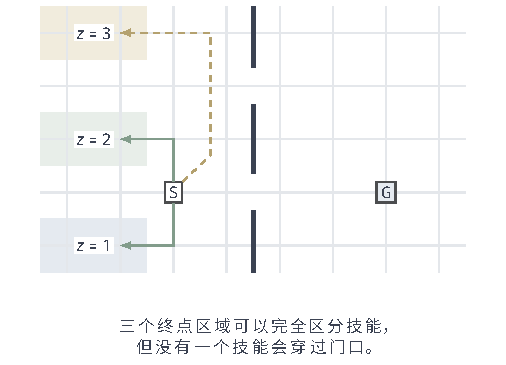
\includegraphics[width=85.750mm]{figures/10-reinforcement-learning/01-problems-and-solving/tikz/rl-learning-skill-regions.pdf}
  \caption{多样但不能完成跨房间任务的技能集合。三种填充和文字标识表示三组不同终点，所有内部策略都限制在墙左侧。可区分性并未提供穿门技能，也未保证一个技能的终点落入另一个有用技能的启动集。}
  \label{fig:rl-learning-skill-regions}
\end{figure}

即使已经有穿门技能，组合还需要启动集相容、终点分布合适和终止时机可靠。评价复用不能只看无奖励阶段相应技能标签与后果之间的互信息或访问区域覆盖面积，还要计入下游技能选择、微调和新增交互成本。这些跨任务问题在第\ref{chap:rl-transfer}章继续展开；时间抽象能改变搜索和学习的单位，但没有取消覆盖、估计与优化三方面的条件。

% Outline: 3.7
\section{样本复杂度与可学习边界}
\label{sec:rl-learning-statistical-limits}

前面给出了经验如何进入更新，也列出了渐近收敛条件。有限预算还需要回答另一个问题：在声明的环境族中，多少真实反馈足以保证输出策略近优，或控制学习期间的回报损失？达到指定策略保证所需的转移样本量，取决于访问协议、问题族和候选函数类。重复梯度与模型生成经验只重复利用已有证据，不能增加这些保证所计数的真实样本。

% Outline: 3.7.1
\subsection{保证对象与数据访问模型}
\label{sec:rl-learning-guarantees-access}

若目标是在训练后得到可部署策略，就应控制输出的次优度，而非仅控制某次训练误差。设算法用$N$次环境反馈输出$\widehat\pi_N$，参照$\pi^*$是在声明策略类中最大化$J$的策略。给定可接受损失$\epsilon$与失败概率$\delta$，大概近似正确（probably approximately correct, PAC）目标把两种要求分开：近似要求回报差不超过$\epsilon$，大概正确要求训练成功概率至少为$1-\delta$。折扣PAC目标要求训练随机性以至少$1-\delta$的概率产生损失不超过$\epsilon$的输出：
\begin{equation}
 \mathbb P\{J(\pi^*)-J(\widehat\pi_N)\leq\epsilon\}
                       \geq1-\delta.
 \label{eq:rl-learning-pac}
\end{equation}
概率覆盖训练记录及算法随机性；$J$本身已经对部署环境取期望。若限制参照为某函数类诱导的策略，就只能称为该类内的近似最优，不应写成全局最优。允许输出一个在回合开始随机选择成员的策略混合时，还应明确这个随机化接口，而不是默认为单个最后网络。

例如$\epsilon=0.1,\delta=0.05$表示：若反复重新采样并训练，至少$95\%$的训练结果应具有不超过$0.1$的期望回报损失。它不要求每条部署轨迹都只损失$0.1$；即使输出策略满足保证，某次滑移仍可能产生很差的实际回报。训练成功事件的概率与固定策略运行后的回报随机性处于两层，下面的遗憾又评价学习期间的全部决策。

有限时域设有$K$回合，每回合$H$步，$T=KH$。记算法第$k$回合使用策略$\pi^{(k)}$，其起点为$s_0^{(k)}$，常见累积伪遗憾为
\begin{equation}
 \operatorname{Reg}_K
   =\sum_{k=1}^{K}\left[
       V_0^*(s_0^{(k)})-V_0^{\pi^{(k)}}(s_0^{(k)})\right].
 \label{eq:rl-learning-episodic-regret}
\end{equation}
每项是给定本回合决策规则后的期望价值差，不是最优期望减去某条实际轨迹的偶然回报。前者关注整个学习过程付出的代价；式\eqref{eq:rl-learning-pac}只关注最终输出。表\ref{tab:rl-learning-guarantee-objects}把容易混淆的量分开。

\begin{table*}[t]
  \centering
  \small
  \begin{tabularx}{\linewidth}{>{\raggedright\arraybackslash}p{24mm} >{\raggedright\arraybackslash}X >{\raggedright\arraybackslash}X}
    \toprule
    保证对象 & 数学陈述或测量量 & 必须说明的输出条件 \\
    \midrule
    PAC输出 & 概率至少$1-\delta$时次优度不超过$\epsilon$ & 固定预算或停止规则；参照类；单策略还是混合策略 \\
    累积遗憾 & $\operatorname{Reg}_K\leq B(K,\delta)$，或其期望界 & 交互过程中全部回合；高概率与期望界不可互换 \\
    Simple regret & 输出次优度$\Delta_N=J^*-J(\widehat\pi_N)$ & 可报告$\mathbb E\Delta_N$或高概率界，须区分二者 \\
    策略识别 & $\mathbb P(\widehat\pi\in\Pi^*)\geq1-\delta$ & 精确识别通常依赖正间隙；等价最优策略可能不唯一 \\
    最后迭代 & 对$\pi^{(K)}$本身保证次优度 & 平均遗憾小不排除最后一轮很差，不能用混合输出替代 \\
    \bottomrule
  \end{tabularx}
  \caption{有限交互样本保证的对象。渐近收敛、PAC输出、学习过程遗憾与最后迭代性质回答不同问题。}
  \label{tab:rl-learning-guarantee-objects}
\end{table*}

例如在固定初始分布下，若平均伪遗憾不超过$\epsilon$，均匀抽取一个已执行策略作为输出，其条件期望次优度不超过$\epsilon$；这还不是概率$1-\delta$的PAC结论。要得到高概率选择，可增加独立评价与置信控制，或使用专门的在线到批量转换。平均策略参数也不等于随机选择策略的混合，神经网络尤其如此。

同一个输出保证，在不同访问能力下可能需要不同样本数。理论中的\term{生成模型}（generative model）是查询预言机：可指定任意合法$(s,a)$，得到独立的真实后继和奖励样本；它不是用有限交互记录训练出的预测模型。基准网格中，这个预言机可直接采样$(4,2)$向上的后果，在线智能体却必须从$(1,1)$先到达那里，还可能滑移。表\ref{tab:rl-learning-access-models}区分查询和实际到达的代价。

\begin{table*}[t]
  \centering
  \small
  \begin{tabularx}{\linewidth}{>{\raggedright\arraybackslash}p{25mm} >{\raggedright\arraybackslash}X >{\raggedright\arraybackslash}X}
    \toprule
    访问协议 & 允许的查询 & 样本保证必须承担的困难 \\
    \midrule
    生成模型 & 指定任意状态动作，抽真实独立转移 & 仍要估计小差异，但免去实际到达目标状态的代价 \\
    在线回合 & 每回合从约定分布或对手给定起点开始 & 必须通过动作取得覆盖，回合内不能任意跳到未见状态 \\
    单条持续轨迹 & 不任意重置，后续状态承接前一动作 & 可达性、返回时间和陷阱；平均奖励常需通信性等条件 \\
    低适应轮数 & 每轮批量采样规则先确定，轮间才能按新取得的转移与奖励记录调整 & 即使总样本相同，反馈轮数有限也可能增加探索成本 \\
    \bottomrule
  \end{tabularx}
  \caption{样本数只有放在访问协议中才有意义。低适应轮数是对查询反馈节奏的附加约束，可以叠加到回合或生成模型协议上。}
  \label{tab:rl-learning-access-models}
\end{table*}

“样本高效”至少应补成一条可检验的任务说明。例如，折扣版本可以是：有限$n_S=|S|,n_A=|\mathsf A|$、奖励在$[0,1]$、$\gamma=0.9$、有生成模型，以概率$0.95$输出满足$J^*-J\leq0.1$的策略，并报告总查询数。有限时域版本应改为$H=20$、$V_H=0$、在线回合采样，以及有限时域价值差；它的回报上界为20，而不是$1/(1-\gamma)=10$。平均奖励版本则需给出持续轨迹、通信MDP及例如直径$D_{\mathrm{diam}}$的条件，以长期增益$g^\pi$或$Tg^*-\sum_{t<T}r_t$为目标，不能沿用折扣$J$。

这些数字只是协议填写示例，不是某算法已达到的实验结果。后文为比较理论将分别声明奖励范围；这也不改变基准网格原有的负步成本。若论文用$K$表示回合数而另一篇用$T$表示时间步，须先代入$T=KH$。同样，按每步奖励不超过1和按整回合总奖励不超过1推导的界，会有不同的时域依赖。

\paragraph{奖励后给定的两阶段探索}
\label{sec:rl-learning-reward-free}
预先围绕一个奖励探索，可能不够支持之后的另一个任务。设机器人先勘查两条通道，再由用户指定配送区域。勘查时没有任务奖励，不能按当前已知高回报路线集中采样；需要先取得能比较未来任务动作后果的转移记录。这就是奖励无关探索要分开的两项工作：先决定访问哪里，再在给定任务奖励后决定怎样行动。

固定非空有限状态集$S$、共同非空有限动作集$\mathsf A$、整数时域$H\geq1$、初始分布$\mu_0$和未知转移核$T_t$，$0\leq t<H$。探索只能按回合从$\mu_0$启动并沿真实状态转移，不能任意跳到待查状态；它观察完整状态，但不使用任务奖励。采集结束后保留有限转移轨迹记录组
$D=(Z_1,\ldots,Z_n)$，其中
$Z_i=(s_{i,0},a_{i,0},\ldots,a_{i,H-1},s_{i,H})$。
规划阶段给出完整的确定性奖励函数组
$R=(R_0,\ldots,R_{H-1})$，每个
$R_t:S\times\mathsf A\to[0,1]$均可计算；允许的全部这类函数组记为$\mathcal R_{\mathrm{task}}$。规划规则只用$D,R$输出$\widehat\pi_{D,R}$，不再采集新的环境轨迹。目标改为有限时域、无折扣回报
$J_H^R(\pi)=\mathbb E_\pi\sum_{t=0}^{H-1}R_t(s_t,a_t)$，
$J_H^{R,*}$是在该任务全部合法策略中的最优值。

奖励可能在看过勘查结果后才确定，所以对某个事先固定奖励的置信保证还不够。给定$\varepsilon,\delta\in(0,1)$，所需的是同一探索事件对所有允许奖励有效：
\begin{equation}
 \mathbb P_{\mathrm{Explore}}\!\left\{
  \sup_{R\in\mathcal R_{\mathrm{task}}}
     [J_H^{R,*}-J_H^R(\widehat\pi_{D,R})]
       \leq\varepsilon\right\}\geq1-\delta.
 \label{eq:rl-learning-reward-free-goal}
\end{equation}
概率针对探索采样及算法随机性；$J_H^R$已经对部署时的状态转移取期望。上确界覆盖全部后给定奖励，而非按某个未声明的奖励分布取平均。一次采集若满足此事件，之后多次更换允许的奖励也无需为这些规划请求再次收集轨迹。

\begin{example}[两条通道与后给定奖励]
 \label{ex:rl-learning-reward-free-branches}
 另设两步确定性教学任务：起点$s_0$选择左或右，第二步任意动作后终止，第一步奖励恒为0。状态集合包含$L,R,B$三个可能后继；两种允许环境中，左动作都到$L$，右动作却分别到$R$和$B$。之后给出的任务甲只在第二步位于$L$时得1，其余为0；任务乙在第二步位于$L,R,B$时分别得$1/2,1,0$。这两套完整奖励函数在两环境中相同，不透露右动作的实际后继。

 若探索只执行左动作，两环境给出相同日志。任务乙中，右到$R$时应选右，右到$B$时应选左，选错都损失$1/2$。即使规划器以概率$q$选择右，两环境的次优差也分别为$(1-q)/2$和$q/2$，至少一个不小于$1/4$。因此同样的左通道日志不能在两环境中都支持误差小于$1/4$的任务乙策略。

 若左右各勘查一次，确定性假设使两个首动作的后果都已确定。任务甲选左得1；任务乙在右通往$R$时选右得1，在右通往$B$时选左得$1/2$，规划时均不用再执行新试验。两条记录足够来自本例的确定性与简单结构；随机通道需要更多样本估计后继概率，不能将这个次数推广为一般保证。
\end{example}

Jin等在有限表格、有限时域设定下构造了满足这种统一保证的探索与规划算法，并给出多项式回合样本上界。其探索先为不同的状态和时刻学习到达策略，再将这些策略组合采样，并在到达后尝试不同动作。用于寻找某状态的指示奖励由探索器自行指定，不是尚未揭示的任务奖励。规划再由记录估计转移，接入给定奖励的近似MDP求解器。覆盖要求按状态在某策略下的最大到达概率调整；对任何策略都极难到达的状态，可将其合计回报影响控制在误差预算内，因此不要求均匀访问全部状态\scite{rl3-jin2020rewardfree}

技能互信息高只说明行为后果可区分，没有给出式\eqref{eq:rl-learning-reward-free-goal}的任务保证；目标重标记也只重算已有转移在另一目标下的奖励。奖励无关探索则把取得足够转移覆盖本身作为前阶段任务，其代价须计入总交互数。这个表格结论不自动扩展到任意潜在表示或神经环境模型。

% Outline: 3.7.2
\subsection{表格MDP的样本复杂度与遗憾}
\label{sec:rl-learning-tabular-complexity}

有限状态动作可以逐对计数，因此探索能直接利用各处尚余的统计不确定性。未充分访问的动作暂留较高估值；真实访问更新经验奖励、转移和置信半径，证据增多后高估值逐渐降低。要让这项不确定性产生远处探索行为，还需通过Bellman备份传回当前可选动作。图\ref{fig:rl-learning-optimistic-grid}将计数与乐观备份并列，说明采样和决策怎样相接。

\begin{figure*}[t]
  \centering
  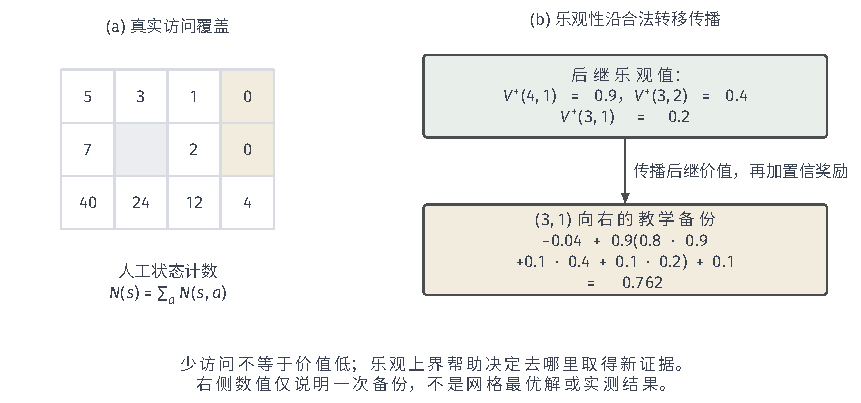
\includegraphics[width=145.750mm]{figures/10-reinforcement-learning/01-problems-and-solving/tikz/rl-learning-optimistic-grid.pdf}
  \caption{计数通过乐观备份影响上游决策。左侧是基准网格合法状态上的人工访问次数，不是实验热图；右侧用一条合法的向右转移说明未知后继的高估值如何影响当前动作。图中折扣教学备份不是下面有限时域UCBVI定理的数值实验。}
  \label{fig:rl-learning-optimistic-grid}
\end{figure*}

E$^3$区分在已知区域利用与主动走向未知区域的策略；R-MAX把不够了解的状态动作暂时接到乐观的高奖励模型\scite{rl3-brafman2002rmax}
两者的重要思想是：无法证明当前策略已经足够好时，就要能以足够概率取得能区分候选环境的新转移或奖励记录。其原始PAC型结果需要声明有限规模、奖励界，以及所用有效时域或混合条件，不能从“模型乐观”直接推出任意持续任务的保证。

回合重置并非每个任务都可用。UCRL2转向持续平均奖励MDP，并要求通信性，即每个状态都能由某种策略到达其他状态。为量化到达代价，定义
$D_{\mathrm{diam}}=\max_{s,s'}\min_\pi\mathbb E_s^\pi\tau_{s'}$
为直径，其中$\tau_{s'}$是到达$s'$的时间。有限$D_{\mathrm{diam}}$排除了某些不可逆陷阱。它在奖励与转移置信集合中选择乐观模型，并按访问计数增长重新规划；在状态与动作集合已知且有限、规模分别为$n_S,n_A$，奖励与转移规律未知、奖励取值位于$[0,1]$的设定下，原论文给出高概率
$\widetilde O(D_{\mathrm{diam}}n_S\sqrt{n_AT})$遗憾界。这个$D_{\mathrm{diam}}$不能用回合长度$H$不加说明地替换\scite{rl3-jaksch2010ucrl2}

\begin{table*}[t]
  \centering
  \small
  \begin{tabularx}{\linewidth}{>{\raggedright\arraybackslash}p{20mm} >{\raggedright\arraybackslash}X >{\raggedright\arraybackslash}X}
    \toprule
    方法 & 保证目标及访问方式 & 乐观机制与必要条件 \\
    \midrule
    E$^3$ & 有限MDP的PAC型学习，原分析包含有效时域与混合条件 & 已知区域评价与到达未知区域的探索规划分开 \\
    R-MAX & 有限MDP近最优学习；平均奖励表述依赖适当混合时间参数 & 不足计数的状态动作给予最大回报的乐观模型 \\
    UCRL2 & 无重置的持续任务遗憾 & 有限直径的通信MDP，奖励和转移置信集合上规划 \\
    UCBVI & 固定长度在线回合的遗憾 & 经验转移与价值置信奖励；下述结果使用时齐转移 \\
    \bottomrule
  \end{tabularx}
  \caption{表格探索保证的任务条件。PAC与遗憾不能只按一个样本数排列，持续任务与回合任务也不具有相同访问能力。}
  \label{tab:rl-learning-tabular-methods}
\end{table*}

理解遗憾界的数量级，可以先看平方根关系。若累积损失主项随$\sqrt T$增长，平均每步损失就随$1/\sqrt T$下降；总试验代价仍在增加，单位时间的代价却逐渐减小。后面用$O$记只关注数量级的上界，$\widetilde O$还省略对数因子；这两种记法都不表示所有预算下实际损失等于主项。显式的次要项和成立条件仍决定有限预算时能用哪个结论。

表\ref{tab:rl-learning-tabular-methods}中的UCBVI直接在经验Bellman备份上加置信奖励。为展示一个具有明确时域依赖的结果，以下固定原论文的设定：$n_S$个状态、每状态$n_A$个动作、已知确定性奖励$R(s,a)\in[0,1]$、未知时齐转移$T$，每回合$H$步，$V_H=0$，没有任意状态查询；回合起点可以由环境选定。第$k$回合前的总访问数为$N^{(k)}(s,a)$，经验转移为$\widehat T^{(k)}$。因为真实$T$不随回合内时刻改变，转移样本可跨时刻合并；若每个时刻有独立$T_t$，统计维数与界会改变。

这一有限时域目标没有折扣，后继价值按剩余步数直接加入。反向计算时，先以经验转移平均后继值，再加置信奖励得到上界；取合法动作的最大值来选择较高回报。还用全程上限$H$和历史上界限制估值，典型更新为
\[
 Q_t^{(k)}(s,a)
   =\min\left\{Q_t^{(k-1)}(s,a),\,H,\,
       R(s,a)+\widehat T^{(k)}V_{t+1}^{(k)}(s,a)
                         +b_t^{(k)}(s,a)\right\},
\]
$V_t^{(k)}=\max_aQ_t^{(k)}$；未访问项保持乐观上限。设共运行$K$回合，真实步数$T=KH$，允许失败概率$\delta\in(0,1)$；以下$L=\log(5Hn_Sn_AT/\delta)$是同时控制各回合、时刻和状态动作的对数参数，不是前面模型滚动的长度。更低的允许失败概率会增大$L$，因而扩大置信半径。简单Hoeffding半径取$H\sqrt{L/N}$量级能说明机制，但不能冒领Bernstein--Freedman（BF）版本的较好界。BF使用后继价值的经验方差，并对随机估值引入额外校正。记$N=N^{(k)}(s,a)>0$、$\widehat T=\widehat T^{(k)}(\cdot\mid s,a)$，
$n_{t+1}^{(k)}(y)$为先前回合在相应时刻访问状态$y$的次数，写出其三个部分：
\begin{align}
 b_t^{(k)}(s,a)
  &=\sqrt{\frac{8L\operatorname{Var}_{\widehat T}
                                  (V_{t+1}^{(k)})}{N}}
       +\frac{14HL}{3N}\notag\\
  &\quad+\sqrt{\frac{8}{N}\sum_y\widehat T(y)
         \min\left\{
           \frac{100^2H^3n_S^2n_AL^2}{n_{t+1}^{(k)}(y)\vee1},H^2
                  \right\}} .
 \label{eq:rl-learning-ucbvi-bonus}
\end{align}
这里数值记号$x\vee1=\max\{x,1\}$，使后继状态计数为0时分母仍至少为1，不表示逻辑“或”。第一项按经验后继价值方差设平方根半径，第二项是有限样本范围修正，第三项补偿估值本身由同批转移记录拟合造成的误差；其中求和按经验后继分布平均，各状态的修正取计数界与$H^2$中较小者。零次计数仍以乐观上限处理，末端已知零价值无需估计。若省去第三项，就不能把由同批转移记录拟合的$V_{t+1}^{(k)}$方差直接当成固定真实价值的方差来使用原保证。

\begin{theorem}[UCBVI-BF的一个有限时域遗憾界]
  \label{thm:rl-learning-ucbvi}
  设状态数$n_S\geq1$、每状态动作数$n_A\geq1$、回合长度$H\geq1$及回合数$K\geq1$均为整数，$T=KH$。奖励为已知确定性函数$R(s,a)\in[0,1]$，未知环境转移核时齐；每回合从环境给定起点在线交互$H$步，终值$V_H=0$，不能任意查询其他状态。取$\delta\in(0,1)$及$L=\log(5Hn_Sn_AT/\delta)$。采用UCBVI-BF原算法，正计数项的置信奖励为式\eqref{eq:rl-learning-ucbvi-bonus}，零计数项保持乐观上限$H$。以至少$1-\delta$的概率，
  \begin{equation}
    \operatorname{Reg}_K
      \leq30L\sqrt{Hn_Sn_AT}
          +2500H^2n_S^2n_AL^2
          +4H\sqrt{TL}.
    \label{eq:rl-learning-ucbvi-bound}
  \end{equation}
  这里的遗憾为式\eqref{eq:rl-learning-episodic-regret}的回合价值差之和。次要项没有被并入主项；只有在相应大样本区域，才适合用
  $\widetilde O(\sqrt{Hn_Sn_AT})$概括其主导尺度。
\end{theorem}

该结果来自Azar、Osband与Munos的定理2；其以回合数表示的首项为$30HL\sqrt{n_Sn_AK}$，末项为$4H^{3/2}\sqrt{KL}$，代入$T=KH$后得到上式。下面解释证明的四个支点，不将简化推导替代原论文对常数和次要项的完整处理\scite{rl3-azar2017ucbvi}

\paragraph{置信事件支持反向乐观性}
加上置信奖励的价值备份首先要成为真实价值的上界，才能指导探索。因此需在奖励已知的设定下，对全部回合、时刻和状态动作同时建立转移集中事件，而不仅保证当前所选动作。由$V_H=0$反向归纳，控制
$(\widehat T-T)V^*_{t+1}$以及同批转移记录拟合的估值带来的额外项，证明
$V_t^{(k)}\geq V_t^*$。对动作取最大保留上界；在多个历史上界中取最小也保留上界，因为它们在同一事件上均不低于真实值。只控制当前访问点，或只控制一个预先固定价值函数，均不足以完成对依赖同批转移记录的估值所作的整段归纳。

\paragraph{把回合损失分成奖励与鞅差}
乐观性使$V_0^{(k)}-V_0^{\pi^{(k)}}$足以覆盖本回合真实遗憾。沿实际访问轨迹展开Bellman关系，后继价值差的条件平均与本次实现之间留下零条件均值的随机项，这就是鞅差；其余由置信奖励和误差修正控制。相邻价值项逐步抵消后，只需累加实际访问处的这些量，不必每回合对全部$n_Sn_A$项重复付出误差。因此，下一步可以利用各处访问次数，而非仅按总时长给粗界。

\paragraph{用访问数而非时间粗界}
对同一状态动作反复访问，平方根半径大致按本地次数$n^{-1/2}$下降。将这一串递减半径求和，再合并全部状态动作的访问预算，关键关系为
\[
  \sum_{n=1}^{m}\frac1{\sqrt n}\leq2\sqrt m,\qquad
  \sum_{n=1}^{m}\frac1n\leq1+\log m,\qquad
  \sum_{s,a}\sqrt{N_T(s,a)}\leq\sqrt{n_Sn_AT}.
\]
前两个界分别控制平方根半径和逆计数修正；最后一步用Cauchy--Schwarz及$\sum_{s,a}N_T(s,a)=T$将各处次数合并。这也说明半径缩小所依据的是新的真实访问，不能用重复训练次数代替没有增加的观测数。

\paragraph{用方差避免多付一个时域因子}
计数求和仍需知道每个半径的尺度。若每步都仅用后继价值范围$H$给界，就忽略了整回合随机性的共同限制，累计时会多付时域因子。BF分析利用沿轨迹的条件方差总和与总回报方差的关系，并用Freedman不等式控制鞅项；随机估值另由式\eqref{eq:rl-learning-ucbvi-bonus}末项校正。将方差累计与访问计数结合，得到$\sqrt{Hn_Sn_AT}$主项，罕见状态和估值修正仍保留为显式次要项。

在相同在线、有限、时齐模型的适当非退化参数及足够大$T$范围内，存在问题族使最坏情形期望遗憾至少为$c\sqrt{Hn_Sn_AT}$量级，$c>0$为通用常数；因此上述主项对$n_S,n_A,H,T$的依赖有相应辨识困难支撑。这是期望下界与高概率上界的尺度比较，不是把两者概率陈述视为相同。若允许每个时刻独立变化的转移核，或者用整回合奖励归一化，必须重新比较，不应引用同一式子。第\ref{sec:rl-learning-statistical-lower}节再用可完整计算的问题对解释下界如何产生。

% Outline: 3.7.3
\subsection{结构化函数逼近的样本效率}
\label{sec:rl-learning-linear-complexity}

图像或连续状态中几乎每次观测都不同，逐状态计数无法等到每处充分访问。跨状态共享样本需要可检验的结构，而不是仅让网络在未见状态动作对上给出较小的预测误差。线性价值近似只规定预测形式；线性MDP进一步要求奖励与转移共同由已知特征线性表示，使各种后继价值的备份也留在同一特征空间。下面区分这种结构与线性混合模型，避免把名称中的“线性”当成相同保证。

仅用线性网络预测价值，约束的是一个函数的形状；让转移具有线性结构，约束的是全部动作后果。一个容易理解的特例是用两个已知非负特征，和为1，混合两份未知后继分布。给定$(s,a)$，特征决定两份分布各占多少；任何后继价值$V$的期望都按同样权重混合，所以换一个$V$仍能用原特征表达。一般线性MDP允许更广的测度表示，但始终要求最终转移是合法概率分布。正是这种对所有后继测试函数都保留的结构，让中间Bellman目标可以共享样本。

\begin{definition}[线性MDP与线性混合MDP]
  \label{def:rl-learning-linear-mdp}
  设$H,d\geq1$为整数，$S$为可测状态空间，合法状态动作域可测。在时刻$t=0,\ldots,H-1$，已知可测特征
  $\bm\phi(s,a)\in\mathbb R^d$，存在未知参数$\bm\theta_t\in\mathbb R^d$和有限有符号测度组成的向量$\bm\mu_t=(\mu_{t,1},\ldots,\mu_{t,d})$使
  \[
    R_t(s,a)=\bm\phi(s,a)^\top\bm\theta_t,\qquad
    T_t(B\mid s,a)=\bm\phi(s,a)^\top\bm\mu_t(B)
  \]
  对每个时刻$t$、每个合法$(s,a)$及每个可测集合$B\subseteq S$成立，则称为相应特征下的线性MDP。奖励均值有限，转移表达必须对各$B$非负且在$B=S$时等于1。
  线性混合MDP的一种常用形式则是已知基核$T_{t,i}$、未知混合权重$\eta_{t,i}$：
  \[
    T_t(\cdot\mid s,a)=\sum_{i=1}^d\eta_{t,i}T_{t,i}(\cdot\mid s,a),
       \qquad \bm\eta_t\in\Delta_d.
  \]
  更一般的线性混合允许其他系数约束，但仍必须保证最终概率核合法。
\end{definition}

第一种结构把状态动作依赖放在已知特征中，未知的是后继状态上的测度；第二种把每个候选后果分布预先给出，未知的是共享系数。在线性混合下，对给定$V$可计算特征
$(T_{t,1}V(s,a),\ldots,T_{t,d}V(s,a))$，它随$V$改变。在线性MDP下，原特征$\bm\phi(s,a)$不随目标改变。二者都称“线性”，并不表示证明条件可以互换。

线性MDP支持价值泛化的原因可直接推导。对任何有界后继价值$V$，
\begin{equation}
 R_t(s,a)+T_tV(s,a)
   =\bm\phi(s,a)^\top
       \left(\bm\theta_t+\int V(s')\,\mathrm d\bm\mu_t(s')\right).
 \label{eq:rl-learning-linear-backup}
\end{equation}
因此每次Bellman备份都仍是相同特征的线性组合。仅有$Q^*$线性可表示，则只约束一个最终解，不能推出任意中间$V$都满足式\eqref{eq:rl-learning-linear-backup}。

这一闭合关系允许用真实转移回归价值参数，而无需枚举后继状态。LSVI-UCB在每回合开始反向重算旧样本的后继目标，做正则化最小二乘，再按未充分约束的特征方向加置信奖励。对第$k$回合，定义先前同一时刻的特征
$\bm\phi_t^{(i)}=\bm\phi(s_t^{(i)},a_t^{(i)})$，令$Q_H^{(k)}=0$，由$t=H-1$向0计算
\begin{align}
 \bm\Lambda_t^{(k)}
   &=\lambda\bm I+\sum_{i<k}
                         \bm\phi_t^{(i)}\bm\phi_t^{(i)\top},\notag\\
 \bm w_t^{(k)}
   &=(\bm\Lambda_t^{(k)})^{-1}
       \sum_{i<k}\bm\phi_t^{(i)}
       \left[r_t^{(i)}
             +\max_aQ_{t+1}^{(k)}(s_{t+1}^{(i)},a)\right],\notag\\
 b_t^{(k)}(s,a)
   &=b_{\mathrm{conf}}\sqrt{\bm\phi(s,a)^\top
                     (\bm\Lambda_t^{(k)})^{-1}\bm\phi(s,a)},\notag\\
 Q_t^{(k)}(s,a)
   &=\min\{H,\bm\phi(s,a)^\top\bm w_t^{(k)}
                                       +b_t^{(k)}(s,a)\}.
 \label{eq:rl-learning-lsvi}
\end{align}
之后执行$a_t^{(k)}\in\argmax_aQ_t^{(k)}(s_t^{(k)},a)$收集一整回合，将真实记录加入下一轮拟合。上式使用原算法的全程上限$H$；当前回合的后继估值会重新生成旧样本的回归目标，不能把它误解成只更新最新一个样本的固定标签回归。

\begin{figure}[t]
  \centering
  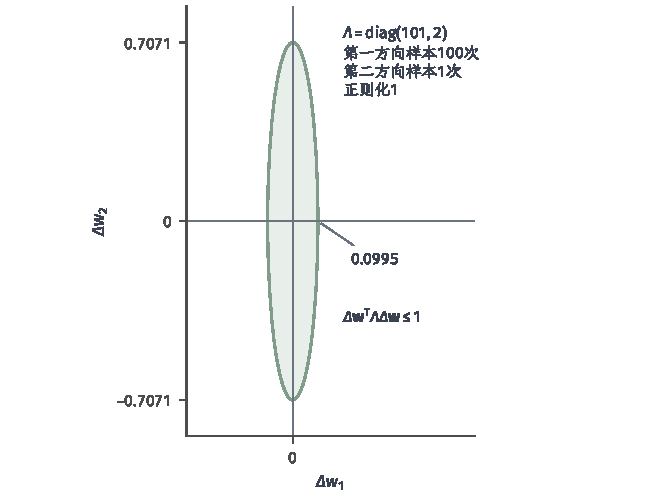
\includegraphics[width=112.000mm]{figures/10-reinforcement-learning/01-problems-and-solving/matplotlib/rl-learning-linear-design.pdf}
  \caption{经验设计矩阵约束的是特征方向。人工例子中$\bm\Lambda=\operatorname{diag}(101,2)$，参数误差椭圆在第一方向很窄、第二方向较宽。即使某个新状态从未出现，只要其特征方向已有充分回归训练样本，置信半径也可能较小。}
  \label{fig:rl-learning-linear-design}
\end{figure}

图\ref{fig:rl-learning-linear-design}中的矩阵来自$\lambda=1$、100个$\bm e_1$样本和一个$\bm e_2$样本。去掉共同系数$b_{\mathrm{conf}}$后，两方向的置信半径分别为
$1/\sqrt{101}\approx0.0995$和$1/\sqrt2\approx0.7071$。半径关心回归训练样本是否约束了该特征方向，而不是网络是否见过该状态动作对。已知特征若没有上述模型实现性，椭圆再窄也可能自信地逼近一个错误模型。

\begin{theorem}[线性MDP中LSVI-UCB的代表性保证]
  \label{thm:rl-learning-lsvi}
  设$d,H,K\geq1$为整数、$\delta\in(0,1)$。考虑可观测状态、有限非空合法动作集、$H$步在线回合，$T=KH$，初始状态允许由环境选择，奖励为确定性$R_t(s,a)\in[0,1]$。真实MDP满足定义\ref{def:rl-learning-linear-mdp}的线性MDP表示，已知
  $\|\bm\phi(s,a)\|_2\leq1$、
  $\|\bm\theta_t\|_2\leq\sqrt d$；为明确测度有界性，取充分条件
  \[
    \left\|\int v(s')\,\mathrm d\bm\mu_t(s')\right\|_2
                          \leq\sqrt d\,\|v\|_\infty
        \quad\text{对所有有界可测 }v.
  \]
  采用$\lambda=1$与充分大的通用常数$c$，令
  $b_{\mathrm{conf}}=c\,dH\sqrt{\log(2dT/\delta)}$。LSVI-UCB以至少$1-\delta$的概率满足
  \[
    \operatorname{Reg}_K
       \leq C\sqrt{d^3H^3T}\log(2dT/\delta)
       =\widetilde O(\sqrt{d^3H^3T}),
  \]
  其中$C$为通用常数。它不需要生成模型访问，也没有显式状态数依赖；动作最大化和特征计算仍必须可执行。
\end{theorem}

这是Jin等人的线性MDP结果；上面将测度规范写成对所有有界测试函数的充分有界条件，避免把有符号测度的总质量与总变差混淆。论文对奖励随机性及模型失配另有讨论，此处不把那些扩展条件省略后并入定理\scite{rl3-jin2020lsvi}

证明沿两条线推进。统计上，式\eqref{eq:rl-learning-linear-backup}使真实备份存在一个范数受控的线性参数；正则化最小二乘的误差可由
$\|\bm\phi\|_{\bm\Lambda^{-1}}$界住。训练转移记录是自适应采集的，后继估值又使用了整批训练记录，因此既要用自归一化鞅集中，也要对算法可能生成的价值类作统一控制，不能把普通独立回归置信区间直接照搬。

决策上，反向归纳得到乐观性，再把遗憾分解为访问轨迹上的置信奖励与鞅项。矩阵行列式引理给
\[
 \det(\bm\Lambda+\bm\phi\bm\phi^\top)
    =\det(\bm\Lambda)(1+\|\bm\phi\|_{\bm\Lambda^{-1}}^2),
\]
所以有限时刻内所有新方向的不确定性总和受$\log\det\bm\Lambda$控制。结合
$\det\bm\Lambda\leq(1+K/d)^d$量级的上界、Cauchy--Schwarz及$H$个时刻的求和，得到累计遗憾界。这是表格访问计数在共享特征空间中的对应物。

该保证约束了整个奖励与转移结构，而不仅是最优值的拟合误差。若任意神经网络在训练样本上能拟合$Q^*$，不能据此认定它具有已知特征、Bellman封闭性、可校准置信半径或高效动作最大化。表示学习可以帮助发现结构，但“能够训练”与“已满足该结构定理”仍是不同判断。

% Outline: 3.7.4
\subsection{一般函数类的可学习条件}
\label{sec:rl-learning-function-classes}

线性MDP的转移结构让中间备份仍可用同一特征表示。一般函数类未必如此：它可能包含最终正确答案，却不能拟合某个候选产生的下一次目标。因此需要分开约束正确答案的可实现性和中间备份的Bellman完备性，而不能只用训练容量回答两者。

先用$\mathcal F_t$记时刻$t$允许选择的价值函数集合，观察“包含答案”与“容纳下一次目标”的差别。

考虑两步、每步一个状态且只有一个动作、奖励全为0的教学任务。取
$\mathcal F_1=\{0,1\}$、$\mathcal F_0=\{0,2\}$，这里集合元素表示常数函数。真实最优值$(Q_0^*,Q_1^*)=(0,0)$在类里；但把候选$f_1=1$备份到前一步得到$\mathcal B_0^*f_1=1\notin\mathcal F_0$。因此可实现不保证每次回归目标可表示。反过来，在该有限时域、固定零终值与相同最优备份算子的完整闭合条件下，可从终点反向推出可实现性；这依赖这些匹配条件，而不是两个术语永远同义。

\begin{definition}[可实现性与Bellman完备性]
  \label{def:rl-learning-realizability}
  设$H\geq1$为整数，$S$为可测状态空间，动作空间$\mathsf A$有限，合法状态动作域可测，各非终止状态的$\mathsf A(s)$非空，终止状态补上零奖励吸收动作，奖励均值可测且有界。有限时域总回报不另加折扣。对$t=0,\ldots,H-1$，$\mathcal F_t$是合法状态动作域上的非空有界可测实函数类，令$\mathcal F_H=\{0\}$及$\mathcal F=\prod_{t=0}^{H-1}\mathcal F_t$。可实现性要求对每个$t$都有$Q_t^*\in\mathcal F_t$。最优Bellman备份定义为
  \[
    (\mathcal B_t^* f_{t+1})(s,a)
       :=R_t(s,a)+\mathbb E_{s'\sim T_t(\cdot\mid s,a)}
                   \max_{a'\in\mathsf A(s')}f_{t+1}(s',a'),
  \]
  其中$t=H-1$的终值项为0。Bellman完备性要求对每个$t$及每个$f_{t+1}\in\mathcal F_{t+1}$，整个备份函数$\mathcal B_t^*f_{t+1}$属于$\mathcal F_t$。若用另一回归类$\mathcal G_t$容纳备份，则相应要求为$\mathcal B_t^*\mathcal F_{t+1}\subseteq\mathcal G_t$，不能省略两个候选类的区别。
\end{definition}

可实现性和完备性仍不直接限制辨识所需样本。庞大候选类若每次观测只排除一个独立候选，就可能需要大量试验；若候选错误共享有限个方向，同一访问分布上的检验可同时约束许多候选。Bellman rank度量探索分布与候选平均Bellman误差之间能否由有限维内积表示，下面正式写出这种分解。

可以把候选检验排成一张表：每一行是一种把智能体带到不同位置的探索策略，每一列是一份待检验价值函数，表项是该候选在这一访问分布下的平均Bellman误差。若表项必须逐个独立检验，所需交互样本数会随表规模增长；若它们能由较少的共同方向表示，一批访问就能约束多个候选。Bellman因子分解把行和列分别映成短向量，再以内积产生表项；分解维数度量这种共享结构，而不是神经网络有多少参数。

\begin{definition}[一种Bellman因子分解]
  \label{def:rl-learning-bellman-rank}
  设$H,M\geq1$为整数、$\zeta\geq0$有限，环境初始分布$\mu_0$和奖励转移核固定，合法动作集有限非空。候选类$\mathcal F$的每个元素为$H$元组$f=(f_0,\ldots,f_{H-1})$，其中各$f_t$为合法状态动作域上的有界可测实函数，约定$f_H\equiv0$；所讨论策略下每步奖励绝对可积。对每个$f\in\mathcal F$和时刻$t$，按固定并列规则选择贪心动作$a_{f,t}(s)$，并令$\pi_f$为它诱导的确定性策略。对$f,g\in\mathcal F$，从$\mu_0$出发，在$t$之前执行$\pi_g$，在$t$及下一步执行$\pi_f$，按环境核生成奖励和后继。定义
  \[
    \operatorname{BE}_t(f,g)=\mathbb E[
       f_t(s_t,a_{f,t}(s_t))-r_t
       -f_{t+1}(s_{t+1},a_{f,t+1}(s_{t+1}))],
  \]
  其中$t=H-1$时最后一项按约定取0，不需在终止后选动作。若对每个$t$都存在映射$\bm\nu_t,\bm\xi_t:\mathcal F\to\mathbb R^M$，使对所有$f,g\in\mathcal F$都有
  \[
    \operatorname{BE}_t(f,g)=\bm\nu_t(g)^\top\bm\xi_t(f),\qquad
    \|\bm\nu_t(g)\|_2\|\bm\xi_t(f)\|_2\leq\zeta,
  \]
  则称该环境与候选类具有维度至多$M$、范数参数$\zeta$的Bellman因子分解。它依赖环境、候选类及生成访问分布的策略，不能理解为网络权重矩阵的秩。
\end{definition}

白话地说，$\bm\nu_t$描述“这次探索把我们带到了哪里”，$\bm\xi_t$描述“这个候选在那里会错多少”，二者通过有限维内积相遇。表格MDP可把状态概率与逐状态误差作为两向量；结构更强时，所需维数可以小于状态数。这种分解不要求算法知道两映射，但证明靠它限制需要多少次有用的排除。

\begin{theorem}[低Bellman rank下的有限类PAC结果]
  \label{thm:rl-learning-olive}
  考虑$H$步在线回合，可从固定初始分布重新开始，动作数为有限$n_A$，每步奖励非负且整回合奖励和几乎处处不超过1。给定有限价值类$\mathcal F$，$|\mathcal F|=N$，函数值在$[0,1]$，终值为0，且真实$Q^*$可实现。假设该类与环境满足定义\ref{def:rl-learning-bellman-rank}的分解，并将范数上界取为$\zeta\geq1$；原上界不足1时可上调为1，不改变分解条件。
  对任意$\epsilon,\delta\in(0,1)$，OLIVE采用原论文阈值与批量样本数，可在
  \[
    \widetilde O\left(
       \frac{M^2H^3n_A}{\epsilon^2}
                         \log\frac{N\zeta}{\delta}\right)
  \]
  个回合内，以至少$1-\delta$的概率输出次优度不超过$\epsilon$的贪心策略。波浪号还隐藏$M,H,n_A,1/\epsilon$的对数项；若按原子环境反馈计数，须再乘$H$。
\end{theorem}

这一陈述是Jiang等人的OLIVE结果在最优值可实现情形下的特例。原框架允许更一般的上下文决策过程及对有效候选类的比较；这里所列特例限定为MDP。其奖励按整回合归一化，不能将该$H$依赖直接与前节每步奖励$[0,1]$的界比较\scite{rl3-jiang2017olive}

OLIVE将这个分解用于候选排除。它在尚未被交互记录否定的函数中选择初始预测回报最高的$f$，再真实执行$\pi_f$检验回报。若预测与实测的差在规定阈值内，且$Q^*$一直未被排除，乐观预测就支持该策略近优；若差距大，则需要找到可检验的错误位置。沿轨迹将候选的相邻价值项抵消，得到
\[
 \mathbb E f_0(s_0,a_{f,0}(s_0))-J_H(\pi_f)
                 =\sum_{t=0}^{H-1}\operatorname{BE}_t(f,f),
\]
其中$J_H$表示该有限时域总回报。故至少一个时刻的Bellman误差足够大。算法按$\pi_f$走到这个时刻，再随机化该处动作，以重要性权重估计其他候选在同一访问分布下的误差，排除与已见奖励和转移记录不一致的候选。

置信阈值保证真实$Q^*$不被误删；分解结构和体积缩减论证保证不能无限产生新的独立错误方向。样本数中的动作因子来自检验时的动作覆盖，函数类大小以$\log N$进入统一集中。但是寻找最乐观候选、检查并维护整个候选集合可能需要枚举$N$个函数；若$N$随输入维数指数增长，样本界小也不等于运行时间小。用神经优化器近似这些步骤，需要额外分析优化与判别误差。

表格MDP给出了这张误差表的一种直接分解：行向量取时刻$t$的各状态访问概率，列向量取该候选在各状态的条件平均残差，两向量内积就是总平均误差。若所有状态的残差还能由少数共享特征控制，就可能进一步降低维数。不同复杂度概念改变的正是“用哪些交互记录、检验哪些候选函数或模型的差异”，下面的比较表沿这一对象区分它们。

\begin{table*}[t]
  \centering
  \small
  \begin{tabularx}{\linewidth}{>{\raggedright\arraybackslash}p{28mm} >{\raggedright\arraybackslash}X >{\raggedright\arraybackslash}X}
    \toprule
    复杂度 & 约束的对象 & 与Bellman因子分解的区别 \\
    \midrule
    Bellman rank & 探索分布与候选Bellman误差之间的有限维因子分解 & 直接约束平均价值一致性，含范数参数和策略类 \\
    Witness rank & 候选模型在测试函数下可被转移记录区分的程度 & 以模型失配的可观测证据为对象，依赖模型类与测试类 \\
    Eluder dimension & 依次出现的新输入上还有多少未被旧观测约束的函数差异 & 点级预测的序贯独立性，不自动包含动力学与Bellman备份 \\
    Bellman--Eluder dimension & Bellman残差类在允许访问分布上的序贯独立性 & 将点级辨识推广到残差及分布，须声明具体分布族 \\
    \bottomrule
  \end{tabularx}
  \caption{几种复杂度各自在控制什么。名称相近不意味着可以把其中一个维数直接代入另一个算法的样本界。}
  \label{tab:rl-learning-function-complexities}
\end{table*}

表\ref{tab:rl-learning-function-complexities}还列出三种相邻概念。Eluder dimension问的是：能否找到很长的新输入序列，使某两个候选在旧输入上几乎一致、在新输入上仍明显不同？它把“还需要多少次新辨识”与函数类的结构联系起来\scite{rl3-russo2013eluder}

Witness rank转向模型：转移记录能否通过某组测试函数见证候选转移与真实转移不一致，且这种证据能支撑策略改进？其条件不是只要求候选价值拟合得好。模型实现性、测试函数族及可执行的模型选择过程都要一并声明\scite{rl3-sun2019witness}

Bellman--Eluder dimension把序贯独立性施加到Bellman残差及访问分布上，覆盖多种可学习问题。相应GOLF或OLIVE分析对实现性、完备性或残差结构的要求随算法而异；低维数不自动解决非凸优化。读这类结果应依次核对“真实问题是否满足结构”“需要多少交互样本”“所需优化能否高效完成”，而不是用一个复杂度名词代替这三项检查\scite{rl3-jin2021bellmaneluder}

% Outline: 3.7.5
\subsection{统计下界与计算—统计差距}
\label{sec:rl-learning-statistical-lower}

上界给出某个算法在声明条件下足以使用的样本量，下界则限制任何算法至少需要的转移或奖励样本。组合锁展示了为什么必须先固定反馈条件：每步若能观察是否走对，就可逐层辨识正确动作；失败与进展若完全不可区分，直到末端才有奖励，一次尝试就难以指出究竟在哪一步选错。图\ref{fig:rl-learning-combination-lock}分开这两种接口，链长$H$本身并不能推出所有算法都需指数样本。

\begin{figure*}[t]
  \centering
  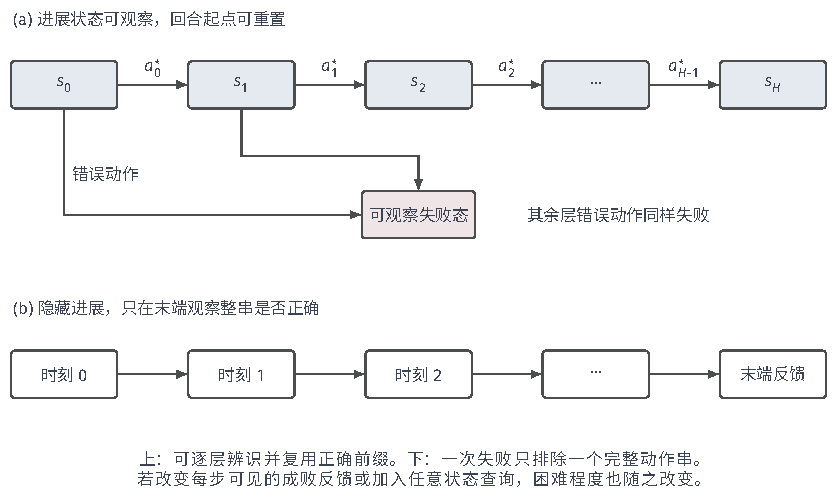
\includegraphics[width=141.750mm]{figures/10-reinforcement-learning/01-problems-and-solving/tikz/rl-learning-combination-lock.pdf}
  \caption{组合锁的难度取决于可观察性与访问方式。上图能观察正确进展或失败状态，只允许回合起点重置；下图把两者隐藏为同一观测，仅整串正确时给终点奖励。后者不是前述完全可观测表格MDP协议。}
  \label{fig:rl-learning-combination-lock}
\end{figure*}

具体地，设每层$n_A$个动作、恰有一个正确动作，确定性转移，错误进入可观察的失败态，下一回合可重置到链首。记住已经验证的前缀后，每层至多试$n_A$个动作，每次走至该层耗$O(H)$步，便有$O(n_AH^2)$步的直接辨识策略；若还有任意状态生成模型查询，连重放前缀也可省去。逐步均匀随机策略偶然成功的概率是$n_A^{-H}$，但这是该策略的表现，不是所有学习算法的下界。

若改成每步只观察时间、失败与进展状态隐藏、非末端奖励均为0，未知正确动作串从$n_A^H$个可能串中均匀选出，那么一次失败仅排除本次完整尝试。每回合最多验证一个串，固定成功概率需要$\Omega(n_A^H)$次尝试。这个教学问题族明确限制了反馈和重置能力；改变成可观察状态或允许查询隐藏状态，论证即不成立。

组合锁改变了观测条件。若仍保留完全可观测的标准设定，也能通过随机奖励的微小差异产生辨识成本。我们构造两个只有一步的环境：近优输出必须选不同动作，单次奖励却难以区分环境。下面将决策要求转换成统计检验，给出可完整计算的样本下界。

两个环境的下界思路与通常估计相反。我们先要求输出必须在两个环境中作出不同选择；再考察训练记录中的动作与奖励能否可靠地区分两个环境。如果大量记录在两环境中仍很相似，就不可能同时高概率选对。这把“策略近优”变成一个环境辨识任务，随后用记录分布的KL计算最多能积累多少证据。

\begin{theorem}[一步决策的辨识下界]
  \label{thm:rl-learning-two-instance-lower}
  设$H=1$、只有一个非终止状态和两个动作。环境$M_+$、$M_-$中动作2奖励均为Bernoulli$(1/2)$，动作1奖励分别为Bernoulli$(1/2+\Delta)$与Bernoulli$(1/2-\Delta)$，其中$0<\Delta\leq1/4$。算法可根据已见历史自适应选择动作，内部随机源在两环境中相同且独立于环境随机性；给定抽样前历史与当前动作，下一奖励仍服从该动作的指定分布。共取得$n\geq1$个奖励反馈后，算法输出任意随机策略。
  若对两环境都以至少$1-\delta$的概率输出$\epsilon$近优策略，其中$\epsilon=\Delta/4$、$0<\delta<1/4$，则
  \[
     n\geq\frac{1}{16\Delta^2}\log\frac1{4\delta}
       =\frac{1}{256\epsilon^2}\log\frac1{4\delta}.
  \]
\end{theorem}

\begin{proof}
  令$\widehat p$为输出策略选择动作1的概率。在$M_+$中$\epsilon$近优要求$\widehat p\geq3/4$；在$M_-$中要求$\widehat p\leq1/4$。故事件$E=\{\widehat p>1/2\}$给出两环境检验，且
  $\mathbb P_+(E^c)+\mathbb P_-(E)\leq2\delta$。

  设$\mathbb P_+,\mathbb P_-$为完整交互记录连同算法随机性的分布。条件于过去，算法使用同一动作选择机制；只有动作1的奖励分布不同。KL的链式法则因此给出
  \[
   D_{\mathrm{KL}}(\mathbb P_+\|\mathbb P_-)
    =\mathbb E_+[N_1(n)]\,
       \operatorname{kl}(1/2+\Delta,1/2-\Delta)
    \leq16n\Delta^2.
  \]
  最后一步利用$\Delta\leq1/4$和
  $\operatorname{kl}(1/2+\Delta,1/2-\Delta)
   =2\Delta\log[(1+2\Delta)/(1-2\Delta)]\leq16\Delta^2$。
  两分布检验不等式
  $\mathbb P_+(E^c)+\mathbb P_-(E)
       \geq\tfrac12e^{-D_{\mathrm{KL}}(\mathbb P_+\|\mathbb P_-)}$
  于是推出$2\delta\geq\tfrac12e^{-16n\Delta^2}$，移项即得结论。
\end{proof}

证明把三个步骤接在一起：奖励均值只差$2\Delta$使单次观测KL为$O(\Delta^2)$；近优策略却必须作出不同选择；检验错误概率将两者连接成样本下界。这里使用的换测度与顺序辨识思路也见最佳臂识别的原始分析，但上面的常数和$\epsilon=\Delta/4$是本书对这一教学问题对的直接推导\scite{rl3-kaufmann2016complexity}

该下界只证明一个状态、两动作、一步任务中已经需要$\epsilon^{-2}$量级奖励样本，不声称导出了前述所有$n_S,n_A,H$因子。多状态MDP下界还需构造多个必须分别辨识的局部选择，并分析访问这些选择与长期收益放大的关系。算法渐近收敛与此不矛盾：对奖励有差异的动作不断采样，最终可以区分两个环境，并不回答在$n$次反馈内能否可靠分清。

\begin{table*}[t]
  \centering
  \small
  \begin{tabularx}{\linewidth}{>{\raggedright\arraybackslash}p{26mm} >{\raggedright\arraybackslash}X >{\raggedright\arraybackslash}X}
    \toprule
    障碍 & 证据要求 & 能从中得出什么 \\
    \midrule
    记录不能区分环境 & 固定访问协议，构造难区分环境及检验下界 & 任何计算能力都不能凭不足的交互记录达到指定保证 \\
    样本有效但计算昂贵 & 有限样本算法依赖枚举大候选类或难解优化 & 当前构造不高效；若要断言所有算法都计算困难，还须规约或计算假设 \\
    计算高效但条件更强 & 如已知线性特征、合法线性转移与可执行动作最大化 & 在该结构族可同时控制交互样本量与计算量，不代表一般网络满足条件 \\
    \bottomrule
  \end{tabularx}
  \caption{可识别性、样本量与计算的边界。算法有昂贵子步骤不等于已经证明计算下界，预言机模型也必须与实际运行成本区分。}
  \label{tab:rl-learning-statistical-computational}
\end{table*}

表\ref{tab:rl-learning-statistical-computational}区分记录可识别、样本充分与计算可行三种判断。OLIVE展示一般结构下的样本可行性，LSVI-UCB在更明确的线性条件下提供可实现的更新，两环境下界则限制任何算法的奖励或转移样本需求。它们各自回答一个问题；只有把访问能力、函数类、目标精度和计算方式一起写出，才有可比较的“可学习”结论。

% Outline: 3.8
\section{算法评估和比较}
\label{sec:rl-learning-evaluation}

实验需要把前述访问能力、表示和预算落实到可复核配置。同一任务上更高的测量回报，可能来自更新机制，也可能来自更多真实交互训练记录、计算、调参或部署搜索。比较前应明确这些差别和评价目标，再报告对应预算下的回报及不确定性；否则一条较高曲线不能区分这些解释。

% Outline: 3.8.1
\subsection{数据与计算预算}
\label{sec:rl-learning-budget}

一条真实转移可以被DQN多次重放，也可以先训练模型，再产生很多合成经验。若只报“训练步”，就会把真实交互样本采集和重复计算混在一起，无法判断样本利用率或运行成本。表\ref{tab:rl-learning-budget-units}分别计真实转移、优化更新、抽样条数和模型查询，训练与部署也单列。

\begin{table*}[t]
  \centering
  \small
  \begin{tabularx}{\linewidth}{>{\raggedright\arraybackslash}p{27mm} >{\raggedright\arraybackslash}X >{\raggedright\arraybackslash}X}
    \toprule
    预算量 & 建议计数方式 & 常见误读 \\
    \midrule
    真实环境步 & 累计实际环境转移；并行环境按各自转移数相加 & 一次向量化调用不等于一次转移，动作重复后的帧数另记 \\
    梯度步 & 按优化器更新次数，并分开行动者、评论家、模型 & 两个评论家的更新不能与单个网络的一步含混合计 \\
    重放比例 & 同时报$U/N_{\mathrm{env}}$及$UB/N_{\mathrm{env}}$，$U$为更新数、$B$为批量 & 前者是更新次数比，后者是抽样条数比，数值相差$B$倍 \\
    模型样本 & 合成转移数、分支起点数与滚动长度分别记录 & 合成100万条不等于真实交互100万次 \\
    墙钟时间 & 固定硬件、并行度，分别记录采集、训练、评价及总耗时 & 只报网络更新时间会漏掉规划、仿真和轨迹采集等待 \\
    参数及内存 & 报可训练参数、目标网络与模型集成数量、峰值内存 & 相同参数数不等于相同计算，回放也占资源 \\
    部署预算 & 每次决策的模型查询、候选数、延迟分位数与硬件 & 训练时省样本可能换来每次动作的大量搜索 \\
    \bottomrule
  \end{tabularx}
  \caption{真实交互记录、记录重放与计算的不同单位。$U,B$随阶段变化时应按各批实际大小累加，不只报一个最终配置值。}
  \label{tab:rl-learning-budget-units}
\end{table*}

可以在基准网格上比较表格Q-learning与学习模型的Dyna，先固定相同的状态、动作、奖励、终止与起点规则。Dyna的模型只能用已取得经验拟合，不能暗中访问本书给出的真实转移表。两者最终都按约定贪心策略部署，探索和学习率的搜索预算相同；Dyna另报告每次真实转移后的模拟备份数。这里选择两种方法只是给出可复现的实验设计，不预先断定哪一个获胜。

一种预算视角固定真实交互数$N_{\mathrm{env}}$：在相同检查点冻结策略，用不进入训练缓冲的独立测试回合估计$J$，比较相同真实环境转移预算下的决策质量。另一种固定总计算资源与墙钟期限：把模型拟合、模拟备份和真实环境执行都计入，比较期限内得到的策略。前者允许算法多花计算提高样本利用率，后者则要求为这些计算付出代价。两种比较回答不同问题，结果不必一致。

部署成本另外测量。网格中两者都可查表选动作；若改成MPC与SAC比较，每次MPC动作的候选搜索应计入部署预算，而SAC的训练开销不应被挪进这一指标。在线更新若与动作生成共享设备，还要报告它是否影响控制延迟。

图\ref{fig:rl-learning-evaluation-protocol}给出两张曲线的作图协议，不包含实验结果。可预先约定20个独立训练种子、每个检查点100个独立测试回合；这些是教学协议的设定值，不是已经完成的运行。第$m$个种子在检查点的测试均值记为$\overline G_m$，保存
$(N_{\mathrm{env}},t_{\mathrm{wall}},\overline G_m)$及测试原始回报，同一检查点分别投到两个横轴，图例始终使用同一算法名与线型。没有实测训练与评价记录时不画领先曲线，也不以手绘趋势代替测量。

\begin{figure*}[t]
  \centering
  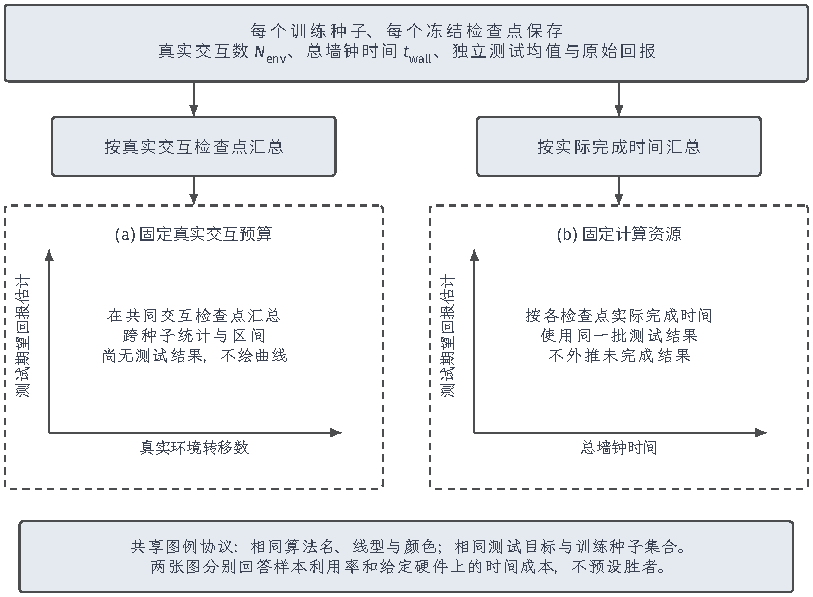
\includegraphics[width=137.615mm]{figures/10-reinforcement-learning/01-problems-and-solving/tikz/rl-learning-evaluation-protocol.pdf}
  \caption{两种预算视角的作图协议，非实验曲线。同一检查点记录同时保留交互数、墙钟时间与测试统计，分别汇总后形成交互预算和时间预算两个视图；方法标识、测试目标和抽样单位保持一致。取得实测训练与评价记录前不填曲线、误差带或排名。}
  \label{fig:rl-learning-evaluation-protocol}
\end{figure*}

画学习曲线还应预先约定插值规则。不同种子的检查点不齐时，可在共同交互预算上使用最近已完成策略，不把尚未达到的结果外推到较小预算；时间轴同理。是否平滑、平滑窗口、失败运行与提前终止如何显示，都要留在作图配置中。曲线下面积若被用作汇总，积分区间与横轴单位也是指标定义的一部分。

% Outline: 3.8.2
\subsection{统计报告与模型选择}
\label{sec:rl-learning-statistical-report}

固定一个训练后的策略测试1000回合，主要减少其环境回报估计的波动；重新训练1000次则还能观察初始化、探索和优化导致的策略差异。要评价算法而非一次幸运训练，必须分开这两个抽样层次，并明确置信区间覆盖哪一种平均性能。这里的学习结果是冻结策略，比较整个学习规则时则重新采集训练记录并重新运行训练程序；两者的期望分别对测试轨迹与训练过程取平均。只有在声明的抽样协议下，独立测试回合才估计对应策略的期望回报，不能把同一训练记录上的自举损失当作测试风险。训练模型与学习规则的两层评价可参考\BookChapterRef{chap:statistical-learning-framework}{卷3《基础、理论与可信性》中讨论机器学习理论基础的章节}。

\Needspace{8\baselineskip}
记第$m$个独立训练运行的冻结策略为$\pi^{(m)}$，第$n$次独立测试回报为$G_{m,n}$。先在每个策略的$N_{\mathrm{test}}$个回合内平均，估计这个产物的期望回报；再对$M$个训练运行平均，估计整个训练流程的平均性能：
\[
 \overline G_m=\frac1{N_{\mathrm{test}}}
                    \sum_{n=1}^{N_{\mathrm{test}}}G_{m,n},\qquad
 \overline G=\frac1M\sum_{m=1}^{M}\overline G_m .
\]
$G_{m,n}$是一次轨迹结果，$\overline G_m$估计这个训练产物的期望性能，$\overline G$估计训练流程随机运行后的平均性能。置信区间应说明覆盖哪一个对象。表\ref{tab:rl-learning-statistical-units}对应这三个层次。

\begin{table*}[t]
  \centering
  \small
  \begin{tabularx}{\linewidth}{>{\raggedright\arraybackslash}p{26mm} >{\raggedright\arraybackslash}X >{\raggedright\arraybackslash}X}
    \toprule
    抽样单位 & 主要随机性与报告量 & 不能替代的统计工作 \\
    \midrule
    单次测试轨迹 & 初始状态、环境噪声和策略采样；报告回报、长度或成功事件 & 一条幸运轨迹不代表该策略的期望性能 \\
    固定训练产物 & 多测试回合的均值与区间 & 不反映重新训练是否会失败 \\
    独立训练运行 & 种子间分布、均值或稳健汇总及区间 & 增加同一种子的测试回合不能消除训练方差 \\
    多任务基准 & 每任务分数、明确归一化后的汇总及性能分布 & 同一模型跨任务测量可能相关，不能当成全部独立样本 \\
    \bottomrule
  \end{tabularx}
  \caption{实验统计的抽样单位。种子列表、测试环境随机数与任务抽样分别记录，置信区间不能只写一个百分比而不说明覆盖对象。}
  \label{tab:rl-learning-statistical-units}
\end{table*}

两层抽样的差别可以量化。若训练产物的真实期望回报方差为$\tau^2$，给定训练产物的轨迹方差再对产物平均为$\sigma^2$，不同训练运行相互独立，且给定各自产物后测试轨迹条件独立同分布，则总方差公式给出
\[
 \operatorname{Var}(\overline G)
   =\frac{\tau^2}{M}
      +\frac{\sigma^2}{M N_{\mathrm{test}}}.
\]
增加$N_{\mathrm{test}}$只压低第二项。学习曲线的相邻检查点来自同一次训练，具有相关性；逐点区间不是“整条曲线同时被覆盖”的置信带，不能用每点95\%宣称整条曲线有95\%覆盖。

取一个教学方差配置$\tau^2=0.04,\sigma^2=0.25$，用$M=5$个训练运行、每个测试100回合，整体均值方差为$0.04/5+0.25/(5\times100)=0.0085$。把每个策略的测试增加到1000回合，只降至$0.00805$；保持100测试回合、把独立训练增加到20次，则降至$0.002125$。这些数说明当训练波动占主导时，反复测试同一模型不能代替重新训练；它们不是某个算法的实测方差。

最少应同时保留学习曲线、预先约定的最终检查点和全部运行的最终分数。跨任务平均前要说明归一化；均值敏感于极端高分，中位数可能掩盖大幅改善或退化，四分位均值（interquartile mean, IQM）取排序后中间50\%分数的平均，提供另一种稳健汇总，但它们没有共同的“正确排名”。

还可用性能分布曲线比较不同分数区域。这里固定一组$M_{\mathrm{task}}$个基准任务，先等概率抽一个任务，再按相同训练协议独立运行该任务的算法，记录预定最终检查点的归一化分数$X$；归一化所用参照也固定。曲线为$\mathbb P(X>\tau)$，表示这一任务与运行混合总体中超过阈值$\tau$的比例，而不是尚未指定的新任务总体。若任务$d$有$M_d$个最终分数$x_{d,m}$，其分层经验估计为
\[
  \widehat{\mathbb P}(X>\tau)
    =\frac{1}{M_{\mathrm{task}}}\sum_{d=1}^{M_{\mathrm{task}}}\frac1{M_d}
       \sum_{m=1}^{M_d}\mathbf1\{x_{d,m}>\tau\}.
\]
每个任务的总权重相同，避免运行较多的任务自动占更大权重；所有$M_d$相同时才等于将全部分数等权合并的尾频率。在同一任务集、预算和归一化下比较曲线，才能判断优势发生在哪些阈值区域。

区间重抽样也应匹配目标。若任务集合固定，按任务分层重抽各任务的训练运行；若关心新任务总体，还需说明任务抽样分布并在外层重抽任务。同一多任务训练产物的多个分数需以整组为单位保留相关性。少量种子下，任何区间估计仍可能很不稳定，应公开原始分数，而不是让一个窄色带制造精确感。Agarwal等人的研究系统讨论了深度强化学习少运行数评价中的区间、IQM和性能分布问题\scite{rl3-agarwal2021precipice}

\begin{example}[挑最好检查点造成的偏差]
  \label{ex:rl-learning-checkpoint-selection}
  假设两个检查点的真实测试均值都为$0.6$，各自的测量误差独立且以相同概率为$\pm0.1$。预先固定最后一个检查点，报告值的期望仍为$0.6$。若看完两次测试后挑较高者，则仅在两次都低时报告$0.5$，其他情形报告$0.7$，所以报告值期望为
  \[
    \frac14(0.5)+\frac34(0.7)=0.65.
  \]
  被选策略的真实均值仍是$0.6$。这$0.05$来自选择噪声，没有任何策略改善。
\end{example}

因此“最好检查点”可以是明确的模型选择协议，却不能在同一批测试轨迹样本上既选又报无偏性能。固定调参候选数、验证预算与选模规则，选择之后另用未参与选择的测试回合评估；若反复查看测试集并改变超参数，测试集已承担验证功能，应另留最终测试。第\ref{sec:rl-learning-dqn}节提到的Rainbow最好快照应按其原协议理解，不与固定最后检查点悄然混比。

消融也需相同预算。去掉组件后若释放大量计算，应说明是保持其他更新次数不变，还是把省下的计算重新分配；前者更接近固定实现条件下的组件作用，后者更接近固定资源下的系统比较。对失败运行不能只删去低分种子，算法性失败应按预先约定纳入分布；基础设施故障的重跑条件和次数另记。

% Outline: 3.8.3
\subsection{基准协议与复现边界}
\label{sec:rl-learning-benchmark-protocol}

使用同名环境也可能取得不同观测字段、执行不同动作或优化不同目标。以ALE为例，像素观测与模拟器内部状态记录属于不同的观测接口；动作重复、黏滞动作、随机起始空操作和生命损失处理还会改变动力学或回合边界。黏滞动作按规定概率继续上一动作，因而固定请求串不再机械复现同一轨迹。比较Atari结果时，需要记录ALE版本、ROM校验值、包装器和黏滞概率，才能确定两种方法面对的是否为同一协议\scite{rl3-machado2018ale}

Procgen有16个程序生成的游戏环境，核心协议之一是限制训练关卡种子，再在未用于训练的关卡上评价。训练与测试关卡重合时测的是另一种泛化问题；难度分布、关卡数、种子区间和版本都要记录。原论文对样本效率和泛化分别给出协议，不能把无限关卡训练与有限关卡训练的分数混在一起\scite{rl3-cobbe2020procgen}

\Needspace{20\baselineskip}
连续控制还需区分状态输入与像素输入、控制周期与底层物理仿真步长、动作重复、奖励缩放以及失败终止。DeepMind Control Suite与Gym中的相近身体模型未必有相同奖励、动作频率或终止条件，名字相似并不能建立直接可比性。其环境定义和任务设计应以具体版本为准\scite{rl3-tassa2018control}

\begin{table*}[t]
  \centering
  \small
  \begin{tabularx}{\linewidth}{>{\raggedright\arraybackslash}p{21mm} >{\raggedright\arraybackslash}X >{\raggedright\arraybackslash}X >{\raggedright\arraybackslash}X}
    \toprule
    基准 & 可见观测字段与动作接口 & 随机性与划分 & 终止及版本记录 \\
    \midrule
    ALE & 像素观测或模拟器内部状态记录、帧堆叠、动作集合、动作重复 & 黏滞动作、随机起始、训练与测试随机种子 & 真正游戏结束、生命损失包装、时间上限；ALE版本、ROM哈希 \\
    Procgen & 像素、动作映射、包装器与网络输入处理 & 训练关卡数、种子区间、未见关卡及难度分布 & 回合结束与截断；包版本、游戏配置、关卡生成种子 \\
    连续控制 & 状态或像素、动作范围、控制频率与重复 & 动力学随机性、初始分布、任务或扰动划分 & 失败终止与时间上限；仿真器、模型文件及任务版本 \\
    \bottomrule
  \end{tabularx}
  \caption{影响算法可读取的观测字段、动力学或目标的基准协议。具体概率和重复次数应从实际配置读取，不把某个流行默认值写成基准的唯一规则。}
  \label{tab:rl-learning-benchmark-settings}
\end{table*}

表\ref{tab:rl-learning-benchmark-settings}中的时间上限尤其容易改变学习目标。沿用第\ref{chap:rl-overview}章的区别，真实终止说明任务后继回报为0；采样截断可能只表示当前记录到此为止。设基准网格中一条非终止转移奖励$-0.04$，后继估值$0.8$，$\gamma=0.9$，若此处只是采样达到时间上限，正确自举目标为$0.68$；错当终止则变成$-0.04$，每次都漏掉$0.72$。若任务本来就定义为到这个时限结束，则零自举才符合目标，且剩余时间通常要进入决策状态。

实现中应分别保存\texttt{terminated}与\texttt{truncated}的含义，并按任务目标确定自举掩码。自动重置的向量环境还须使用截断前的最终观测，不能把下一回合重置后的观测当成这条转移的后继。时间上限的两种语义及其对状态与自举的影响，有专门的原始分析\scite{rl3-pardo2018timelimits}

跨游戏原始分数的单位不同，不能直接把数值大小当成统一性能。若用随机与人类参照对每个游戏缩放，就需要同时固定参照值和测量协议。以ALE常见的人类归一化分数为例，
\[
  S_{\mathrm{HN}}
   =\frac{S_{\mathrm{agent}}-S_{\mathrm{random}}}
          {S_{\mathrm{human}}-S_{\mathrm{random}}}.
\]
必须提供每个游戏的人类与随机参照值及其测量协议。若分母很小，少量原始分差会被放大；若参照顺序反常或分母为0，应说明排除或替代规则，不能直接平均。教学值
$S_{\mathrm{agent}}=30,S_{\mathrm{random}}=10,S_{\mathrm{human}}=50$
对应$0.5$，不是原始得分的“50\%”；它表示从随机到人类参照差距的一半。是否截断到某范围也会改变跨任务汇总，需明确报告。

\begin{table*}[t]
  \centering
  \small
  \begin{tabularx}{\linewidth}{>{\raggedright\arraybackslash}p{28mm} >{\raggedright\arraybackslash}X}
    \toprule
    复现记录 & 最少需要保存的内容 \\
    \midrule
    代码与配置 & 提交标识、依赖锁定、环境与包装器版本、全部实际展开后的超参数 \\
    训练记录、评价样本与随机性 & 真实交互记录与模型合成转移的来源及条数、训练与评价种子、初始分布、训练测试划分 \\
    更新语义 & 采样策略版本、目标网络与策略更新频率、终止掩码、重放比例及样本寿命 \\
    模型选择 & 候选与调参预算、验证集、停止及检查点选择规则、最终独立测试流程 \\
    失败处理 & 失败定义、原始结果、基础设施重跑规则与实际重跑次数 \\
    资源与产物 & 硬件、精度、并行度、墙钟和部署预算、模型检查点、逐运行日志与作图脚本 \\
    \bottomrule
  \end{tabularx}
  \caption{最小复现记录。分布式系统实现可在系统卷展开，但会改变采样分布或更新目标的接口必须在算法实验中说明。}
  \label{tab:rl-learning-reproducibility}
\end{table*}

表\ref{tab:rl-learning-reproducibility}不是附在论文末尾的形式清单：每一项都可能改变结论。例如异步采样器延迟会增大行为策略与目标策略的差别，回放保留期会改变访问分布，模型更新频率会改变合成经验的失配程度。采样服务与分布式存储怎样工程实现留给系统卷；这些实现选择对训练记录抽样分布和更新目标的影响，需要写入实验协议。

% Outline: 3.9
\section{本章小结}
\label{sec:rl-learning-summary}

回到章首网格问题，一次动作只能给出一次奖励和落点，我们既要用它估计长期后果，也要决定下一次去哪里取得证据。本章的四种组合给出了不同计算接口：直接更新价值或策略，或者先学模型，再用预测支持这些更新。表\ref{tab:rl-learning-final-interfaces}按主要更新对象和最终动作来源汇总；混合系统应沿交互记录、模型预测与训练目标之间的实际依赖解释，不能只凭出现了某个网络就归类。

\begin{table*}[t]
  \centering
  \small
  \begin{tabularx}{\linewidth}{>{\raggedright\arraybackslash}p{28mm} >{\raggedright\arraybackslash}X >{\raggedright\arraybackslash}X}
    \toprule
    主要接口 & 经验主要更新什么 & 最终动作主要来自哪里 \\
    \midrule
    无模型价值学习 & MC/TD回报、动作值与其函数表示 & 对动作价值贪心或按约定探索，如SARSA、Q-learning、DQN \\
    无模型策略优化 & 策略参数，通常另有评价策略的评论家 & 更新后的策略，如PPO、SAC；离策略校正与覆盖仍需检查 \\
    基于模型的价值学习与规划 & 动力学、奖励及规划需要的价值或搜索先验 & Dyna更新后的价值控制，或MPC、MuZero、TD-MPC的当前规划结果 \\
    基于模型的策略优化 & 动力学以及用模型梯度或合成转移记录训练的行动者、评论家 & 更新后的策略，如PILCO、Dreamer、MBPO；潜在状态推断仍可调用模型 \\
    \bottomrule
  \end{tabularx}
  \caption{四种组合共享探索、函数表示与时间抽象条件。混合系统按实际交互记录、模型预测与动作选择的依赖说明，不要求每个系统只学习一种对象。}
  \label{tab:rl-learning-final-interfaces}
\end{table*}

这些接口都处在同一反馈中。关键动作样本不足会使回报、转移或价值估计不可靠，估计误差又通过贪心选择或策略更新改变动作，新的访问分布进一步决定哪些误差能被修正。MC需要完整回报，因而通常等待回合结束；TD用一步奖励加后继预测，可以立即更新，却要处理自举误差。离策略评价复用旧策略的记录，还需保留行为动作概率并检查目标行为是否得到支持。它们对记录的要求不同，估计误差的来源也不同。双重采样反例提醒我们先核对损失是否对应目标；资格迹和优势估计改变信用传播长度，却不能补出未取得的奖励反馈。

是否得到可靠策略，取决于误差能否转到实际决策分布。统一动作值误差给出贪心策略损失界，低训练均方误差却可能漏掉关键岔路；性能差恒等式使用新策略占用下的优势，旧批次代理必须控制分布替代；模拟界需要奖励与转移误差覆盖被选策略，而搜索和想象优化恰会寻找高估区域。时间抽象同样保留这些要求：Option用$\gamma^K$维持原子时间目标，高层少做几次决策，并不意味着真实交互、内部控制学习或执行风险同比减少。

有限样本分析进一步把这些条件写成访问协议和问题结构。UCBVI依赖表格计数，LSVI-UCB依赖已知特征及线性奖励转移，OLIVE依赖候选误差的有限维分解；它们分别约束不同问题族，不能拼成任意神经算法的保证。实验相应地需要分别记录真实样本、重复更新、模型计算、选模和部署预算，并用独立训练运行区分训练波动与固定策略的测试波动。

因此，环境模型未知时仍可通过经验评价和改进策略，但一次更新可计算，尚不足以保证有限预算下近优。算法形式规定怎样利用记录，访问能力规定能取得什么记录，函数类规定不同状态动作的记录怎样共同约束价值或模型，预算则限制辨识和求解能做到哪里；四者共同决定策略保证的适用范围。后续各章改变观测与采集权限、奖励反馈、任务、参与者或行为要求，复用这里的部件时也需重新检查其交互记录来源、优化目标和保证条件。
